% Options for packages loaded elsewhere
\PassOptionsToPackage{unicode}{hyperref}
\PassOptionsToPackage{hyphens}{url}
%
\documentclass[
  a4paper,
  oneside,
  openany]{book}
\title{Modelos no paramétricos}
\author{Sofía Villers Gómez \and Dulce María Reyes Varela \and Carlos Fernando Vásquez Guerra}
\date{}

\usepackage{amsmath,amssymb}
\usepackage{lmodern}
\usepackage{iftex}
\ifPDFTeX
  \usepackage[T1]{fontenc}
  \usepackage[utf8]{inputenc}
  \usepackage{textcomp} % provide euro and other symbols
\else % if luatex or xetex
  \usepackage{unicode-math}
  \defaultfontfeatures{Scale=MatchLowercase}
  \defaultfontfeatures[\rmfamily]{Ligatures=TeX,Scale=1}
\fi
% Use upquote if available, for straight quotes in verbatim environments
\IfFileExists{upquote.sty}{\usepackage{upquote}}{}
\IfFileExists{microtype.sty}{% use microtype if available
  \usepackage[]{microtype}
  \UseMicrotypeSet[protrusion]{basicmath} % disable protrusion for tt fonts
}{}
\makeatletter
\@ifundefined{KOMAClassName}{% if non-KOMA class
  \IfFileExists{parskip.sty}{%
    \usepackage{parskip}
  }{% else
    \setlength{\parindent}{0pt}
    \setlength{\parskip}{6pt plus 2pt minus 1pt}}
}{% if KOMA class
  \KOMAoptions{parskip=half}}
\makeatother
\usepackage{xcolor}
\IfFileExists{xurl.sty}{\usepackage{xurl}}{} % add URL line breaks if available
\IfFileExists{bookmark.sty}{\usepackage{bookmark}}{\usepackage{hyperref}}
\hypersetup{
  pdftitle={Modelos no paramétricos},
  pdfauthor={Sofía Villers Gómez; Dulce María Reyes Varela; Carlos Fernando Vásquez Guerra},
  hidelinks,
  pdfcreator={LaTeX via pandoc}}
\urlstyle{same} % disable monospaced font for URLs
\usepackage[top=1in, left=1in, right=1in, bottom=1in]{geometry}
\usepackage{color}
\usepackage{fancyvrb}
\newcommand{\VerbBar}{|}
\newcommand{\VERB}{\Verb[commandchars=\\\{\}]}
\DefineVerbatimEnvironment{Highlighting}{Verbatim}{commandchars=\\\{\}}
% Add ',fontsize=\small' for more characters per line
\usepackage{framed}
\definecolor{shadecolor}{RGB}{248,248,248}
\newenvironment{Shaded}{\begin{snugshade}}{\end{snugshade}}
\newcommand{\AlertTok}[1]{\textcolor[rgb]{0.94,0.16,0.16}{#1}}
\newcommand{\AnnotationTok}[1]{\textcolor[rgb]{0.56,0.35,0.01}{\textbf{\textit{#1}}}}
\newcommand{\AttributeTok}[1]{\textcolor[rgb]{0.77,0.63,0.00}{#1}}
\newcommand{\BaseNTok}[1]{\textcolor[rgb]{0.00,0.00,0.81}{#1}}
\newcommand{\BuiltInTok}[1]{#1}
\newcommand{\CharTok}[1]{\textcolor[rgb]{0.31,0.60,0.02}{#1}}
\newcommand{\CommentTok}[1]{\textcolor[rgb]{0.56,0.35,0.01}{\textit{#1}}}
\newcommand{\CommentVarTok}[1]{\textcolor[rgb]{0.56,0.35,0.01}{\textbf{\textit{#1}}}}
\newcommand{\ConstantTok}[1]{\textcolor[rgb]{0.00,0.00,0.00}{#1}}
\newcommand{\ControlFlowTok}[1]{\textcolor[rgb]{0.13,0.29,0.53}{\textbf{#1}}}
\newcommand{\DataTypeTok}[1]{\textcolor[rgb]{0.13,0.29,0.53}{#1}}
\newcommand{\DecValTok}[1]{\textcolor[rgb]{0.00,0.00,0.81}{#1}}
\newcommand{\DocumentationTok}[1]{\textcolor[rgb]{0.56,0.35,0.01}{\textbf{\textit{#1}}}}
\newcommand{\ErrorTok}[1]{\textcolor[rgb]{0.64,0.00,0.00}{\textbf{#1}}}
\newcommand{\ExtensionTok}[1]{#1}
\newcommand{\FloatTok}[1]{\textcolor[rgb]{0.00,0.00,0.81}{#1}}
\newcommand{\FunctionTok}[1]{\textcolor[rgb]{0.00,0.00,0.00}{#1}}
\newcommand{\ImportTok}[1]{#1}
\newcommand{\InformationTok}[1]{\textcolor[rgb]{0.56,0.35,0.01}{\textbf{\textit{#1}}}}
\newcommand{\KeywordTok}[1]{\textcolor[rgb]{0.13,0.29,0.53}{\textbf{#1}}}
\newcommand{\NormalTok}[1]{#1}
\newcommand{\OperatorTok}[1]{\textcolor[rgb]{0.81,0.36,0.00}{\textbf{#1}}}
\newcommand{\OtherTok}[1]{\textcolor[rgb]{0.56,0.35,0.01}{#1}}
\newcommand{\PreprocessorTok}[1]{\textcolor[rgb]{0.56,0.35,0.01}{\textit{#1}}}
\newcommand{\RegionMarkerTok}[1]{#1}
\newcommand{\SpecialCharTok}[1]{\textcolor[rgb]{0.00,0.00,0.00}{#1}}
\newcommand{\SpecialStringTok}[1]{\textcolor[rgb]{0.31,0.60,0.02}{#1}}
\newcommand{\StringTok}[1]{\textcolor[rgb]{0.31,0.60,0.02}{#1}}
\newcommand{\VariableTok}[1]{\textcolor[rgb]{0.00,0.00,0.00}{#1}}
\newcommand{\VerbatimStringTok}[1]{\textcolor[rgb]{0.31,0.60,0.02}{#1}}
\newcommand{\WarningTok}[1]{\textcolor[rgb]{0.56,0.35,0.01}{\textbf{\textit{#1}}}}
\usepackage{longtable,booktabs,array}
\usepackage{calc} % for calculating minipage widths
% Correct order of tables after \paragraph or \subparagraph
\usepackage{etoolbox}
\makeatletter
\patchcmd\longtable{\par}{\if@noskipsec\mbox{}\fi\par}{}{}
\makeatother
% Allow footnotes in longtable head/foot
\IfFileExists{footnotehyper.sty}{\usepackage{footnotehyper}}{\usepackage{footnote}}
\makesavenoteenv{longtable}
\usepackage{graphicx}
\makeatletter
\def\maxwidth{\ifdim\Gin@nat@width>\linewidth\linewidth\else\Gin@nat@width\fi}
\def\maxheight{\ifdim\Gin@nat@height>\textheight\textheight\else\Gin@nat@height\fi}
\makeatother
% Scale images if necessary, so that they will not overflow the page
% margins by default, and it is still possible to overwrite the defaults
% using explicit options in \includegraphics[width, height, ...]{}
\setkeys{Gin}{width=\maxwidth,height=\maxheight,keepaspectratio}
% Set default figure placement to htbp
\makeatletter
\def\fps@figure{htbp}
\makeatother
\setlength{\emergencystretch}{3em} % prevent overfull lines
\providecommand{\tightlist}{%
  \setlength{\itemsep}{0pt}\setlength{\parskip}{0pt}}
\setcounter{secnumdepth}{5}
\usepackage[utf8]{inputenc}% Usa codificación 8-bit que tiene 256 glyphs
\usepackage[T1]{fontenc}
%Más información de babel : http://www.texnia.com/spanishopt.html
%es-tabla: Traduce table como tabla en lugar de como cuadro.
%es-nodecimaldot: No añade punto tras los números de sección, subsección
\usepackage[spanish,es-nodecimaldot,es-tabla]{babel} 
\usepackage{graphicx} %Manipulación de imágenes : https://es.overleaf.com/learn/latex/Inserting_Images
\usepackage{tikz} % Requerido para dibujar formas personalizadas
\usepackage{float} %Gráficas
\usepackage{fancyhdr} %Para un mejor manejo de encabezados
\usepackage{calc} %Para hacer cálculos matemáticos en Latex
\usepackage{amsmath,amssymb,amsfonts} %Para tener mejores opciones en estructuras matemáticas.
\usepackage{amsthm} %Ambientes matemáticos : http://www.ctex.org/documents/packages/math/amsthdoc.pdf
%Vamos a colocar todo el formato que yihui colocó en su bookdown:https://github.com/rstudio/bookdown/blob/master/inst/examples/latex/preamble.tex
\usepackage{mathrsfs}
\usepackage{booktabs}
\usepackage{longtable}
\renewcommand{\textfraction}{0.05}
\renewcommand{\topfraction}{0.8}
\renewcommand{\bottomfraction}{0.8}
\renewcommand{\floatpagefraction}{0.75}
\usepackage{listings}
\lstset{
  breaklines=true
}
\ifLuaTeX
  \usepackage{selnolig}  % disable illegal ligatures
\fi
\usepackage[]{natbib}
\bibliographystyle{apalike}
\nocite{montgomery2021introduction, conover1998practical, gibbons2020nonparametric}

\begin{document}
\maketitle

{
\setcounter{tocdepth}{2}
\tableofcontents
}
\hypertarget{prefacio}{%
\chapter*{Prefacio}\label{prefacio}}


El curso de Modelos No Paramétricos y de Regresión es el segundo curso de estadística en el mapa curricular de la carrera de actuaría en la facultad, por lo que al llegar a este curso es muy probable que ya hayan cursado inferencia estadística en donde se revisan temas de estimación de parámetros (estimación puntual, estimación por interválos, pruebas de hipótesis sobre las estimaciones de dichos parámetros). Se puede notar que las metodologías estudiadas en el curso de inferencia se basan en el supuesto de que conocemos las distribución que sigue nuestra variable de interes y por lo tanto las observaciones provienen de una cierta familia paramétrica de distribuciones y entonces con las observaciones (muestra) podemos hacer inferencia estadística acerca de los valores de los parámetros de dicha distribución.

Sin embargo, hay casos en donde desconocemos la distribución paramétrica de la que provienen nuestros datos y aún así quiseramos poder realizar algún tipo de inferencia sobre la variable de interes o de la población. ¿Se puede?

La respuesta es sí, pero utilizando procedimientos distintos o realizando algunas variaciones a las metodologías vistas en el curso de inferencia estadística. Esos son los temas que se revisan en la primer parte de este curso denominado modelos no paramétricos.

\hypertarget{objetivos}{%
\subsection*{Objetivos}\label{objetivos}}


\begin{itemize}
\item
  Proporcionar a los alumnos el material para cubrir los temas del curso de modelos no paramétricos y de regresión.
\item
  Reforzar las bases teóricas con contenido electrónico completado con herramientas de R-Studio.
\end{itemize}

Este libro fue escrito con \href{http://bookdown.org/}{bookdown} usando \href{http://www.rstudio.com/ide/}{RStudio}.

Esta versión fue escrita con:

\hypertarget{licencia}{%
\subsection*{Licencia}\label{licencia}}


This work is licensed under a \href{https://creativecommons.org/licenses/by-sa/4.0/}{Creative Commons Attribution-ShareAlike 4.0 International License}.

\emph{This is a human-readable summary of (and not a substitute for) the license.
Please see \url{https://creativecommons.org/licenses/by-sa/4.0/legalcode} for the full legal text.}

\textbf{You are free to:}

\begin{itemize}
\item
  \textbf{Share}---copy and redistribute the material in any medium or
  format
\item
  \textbf{Remix}---remix, transform, and build upon the material for any
  purpose, even commercially.
\end{itemize}

The licensor cannot revoke these freedoms as long as you follow the
license terms.

\textbf{Under the following terms:}

\begin{itemize}
\item
  \textbf{Attribution}---You must give appropriate credit, provide a link
  to the license, and indicate if changes were made. You may do so in
  any reasonable manner, but not in any way that suggests the licensor
  endorses you or your use.
\item
  \textbf{ShareAlike}---If you remix, transform, or build upon the material, you must distribute your contributions under the same license as the original.
\item
  \textbf{No additional restrictions}---You may not apply legal terms or
  technological measures that legally restrict others from doing
  anything the license permits.
\end{itemize}

\textbf{Notices:}

You do not have to comply with the license for elements of the
material in the public domain or where your use is permitted by an
applicable exception or limitation.

No warranties are given. The license may not give you all of the
permissions necessary for your intended use. For example, other rights
such as publicity, privacy, or moral rights may limit how you use the
material.

\hypertarget{part-introducciuxf3n}{%
\part{Introducción}\label{part-introducciuxf3n}}

\hypertarget{introducciuxf3n}{%
\chapter*{Introducción}\label{introducciuxf3n}}


Los métodos paramétricos tienen la caracteristica de que siempre se trabaja con muestras aleatorias provenientes de cierta distribución conocida. Por otro lado, los métodos no paramétricos suelen requerir suposiciones menos restrictivas acerca del nivel de medición de los datos y sobre la forma de las distribuciones de probabilidad generadas por los datos muestrales, por lo que se pueden usar en situaciones en donde los métodos paramétricos no son aplicables.

Una de las consideraciones para determinar si lo apropiado es un método paramétrico o un método no paramétrico es la escala de medición empleada para generar los datos. Todos los datos son generados por una de las cuatro escalas de medición: nominal, ordinal, de intervalo o de razón.

\hypertarget{escalas-de-mediciuxf3n}{%
\chapter{Escalas de Medición}\label{escalas-de-mediciuxf3n}}

Esta sección es una traducción de \citet{conover1998practical}.

A continuación se definirán los tipos de escalas que se le asigna a una variable. Hay cuatro escalas básicas las cuales son: \textbf{nominal, ordinal, de intervalo y de razón.} A las variables que se consideran con escala ordinal y nominal también se les conoce como \textbf{variables categóricas o cualitativas}, mientras que a las variables que se consideran con escala de intervalo y razón se conocen como \textbf{variables cuantitativas}.

\hypertarget{variables-categuxf3ricas}{%
\section{Variables categóricas}\label{variables-categuxf3ricas}}

\hypertarget{escala-nominal}{%
\subsection{Escala nominal:}\label{escala-nominal}}

La escala nominal utiliza números simplemente como un medio para separar las propiedades o elementos en diferentes clases o categorías. El número asignado a la observación sirve sólo como un \textbf{``nombre''} para la categoría a la que pertenece la observación, de ahí el título \textbf{``nominal''}. Por ejemplo, utilizamos la escala nominal de medición cuando definimos una variable aleatoria que equivalía a \(1\) si una moneda caía \textbf{``sol''}, y \(0\) si la moneda caía \textbf{``águila''}. Podríamos, igual bien, haber usado los números \textbf{7.3} y \textbf{3.9} para representar el sol y el águila, respectivamente. Nuestra elección de \(1\) y \(0\) fue principalmente por conveniencia.
Otro ejemplo, cuando 12 sujetos se numeran arbitrariamente del 1 al 12, se utiliza una escala de medición nominal y la asignación de los números es una forma de variable aleatoria. Al clasificar objetos según el color, las categorías pueden etiquetarse como 1, 2, 3 o azul, amarillo, rojo o A, B, C. Los números son simplemente nombres de categoría. Los números pueden ser reemplazados por otros números no utilizados, siempre que las categorías permanezcan intactas.

\hypertarget{escala-ordinal}{%
\subsection{Escala ordinal:}\label{escala-ordinal}}

La escala ordinal se refiere a mediciones en las que sólo son relevantes las comparaciones \textbf{``mayor''},\textbf{``menor''} o \textbf{``igual''} entre ellas. El valor numérico se usa sólo como un medio para organizar los elementos que se miden en orden, de menor a mayor.
Ésta capacidad de ordenar los elementos, en función del tamaño relativo de sus medidas, le da el nombre de
Si algunos de los elementos son iguales entre sí, decimos que existen vínculos. Cuando se le pide a una persona que asigne el número 1 a la más preferida de las tres marcas, el número 3 a la menos preferida y el número 2 a la marca restante, está usando una escala ordinal y está usando los números 1, 2, 3; ésta podría haber usado tres números, digamos 16, 20, 75, siempre y cuando los números se asignen a las marcas de tal manera que el orden relativo del número represente la preferencia relativa de la marca.

\hypertarget{variables-cuantitativas}{%
\section{Variables cuantitativas}\label{variables-cuantitativas}}

\hypertarget{escala-de-intervalo}{%
\subsection{Escala de intervalo:}\label{escala-de-intervalo}}

La escala de intervalo, considera como información pertinente \textbf{no sólo} el orden relativo de las mediciones como en la escala ordinal sino también el \textbf{tamaño del intervalo} entre mediciones, es decir, el tamaño de la diferencia (en un sentido de resta) entre dos mediciones. La escala de intervalo implica el concepto de una unidad de distancia, y la distancia entre dos mediciones cualquiera puede expresarse como un cierto número de unidades. Un buen ejemplo es la escala por la cual generalmente representamos la temperatura. El aumento de una unidad (grado) de temperatura se define por un cambio particular en el volumen de mercurio en un termómetro; en consecuencia, la diferencia entre dos temperaturas cualquiera puede medirse en \textbf{unidades o grados}. El valor numérico real de la temperatura es simplemente una comparación con un punto arbitrario llamado ``cero grados''. La escala de intervalo requiere un punto cero y una unidad de distancia (no es posible tener este último sin el primero), pero no es importante cómo se definan los ``ceros'' y la unidad de distancia.

La temperatura ha sido medida de manera bastante adecuada durante algún tiempo por las escalas Fahrenheit y Celsius, que tienen diferentes temperaturas cero y diferentes definiciones de 1 grado o unidad. El principio de las mediciones de intervalo no se viola por un cambio en la escala o la ubicación o ambos.

\hypertarget{escala-de-razuxf3n}{%
\subsection{Escala de razón:}\label{escala-de-razuxf3n}}

La escala de razón se usa cuando \textbf{no sólo el orden y el tamaño del intervalo son importantes}, sino que también la \textbf{razón entre dos medidas} es significativa. Si es razonable hablar de que una cantidad es ``dos veces'' otra cantidad, la escala de proporción es apropiada para la medición, como cuando se miden los rendimientos de cultivos, distancias, pesos, alturas, ingresos, etc. En realidad, la única distinción entre la escala de razón y la escala de intervalo es que la escala de razón tiene una \textbf{medida natural} ``cero'', mientras que la medida de cero se define \textbf{arbitrariamente} en la escala de intervalo. Como en la escala de intervalo, la unidad de distancia de la escala de razón se define arbitrariamente.

No existe un acuerdo universal entre los científicos que prefieren usar escalas adicionales, y algunas mediciones no se incluyen claramente en una de las cuatro escalas recién definidas.
Por lo tanto, ésta clasificación de escalas de medida puede ser demasiado simplista, pero es suficiente para los propósitos de este curso.

La mayoría de los métodos estadísticos paramétricos habituales requieren una escala de medición de intervalo (o más fuerte). La mayoría de los métodos no paramétricos suponen que la escala nominal o la escala ordinal son apropiadas.

\hypertarget{part-pruebas-binomiales}{%
\part{Pruebas Binomiales}\label{part-pruebas-binomiales}}

\hypertarget{introducciuxf3n-1}{%
\chapter*{Introducción}\label{introducciuxf3n-1}}


La distribución de probabilidad binomial se introdujo para describir las probabilidades asociadas con el número de caras cuando se lanza una moneda \(n\) veces. En su forma más general, cada uno de \(n\) ensayos independientes da como resultado \("éxito"\), con probabilidad \(p\), o \("fracaso"\), con probabilidad \(q = 1-p\). La distribución binomial describe la probabilidad de obtener exactamente \("k"\) éxitos.

\hypertarget{prueba-de-proporciones}{%
\chapter{Prueba de Proporciones}\label{prueba-de-proporciones}}

Supongamos que un científico desea saber si la tasa de mortalidad va en aumento, si la tasa de pobreza está cambiando o si la tasa de algún grupo cívico está a favor de una política en particular. En muchos casos existe una proporción hipotética \(p\) de una población en estudio y una poporción específica \(p^*\) y se pretende llevar a cabo una comparación para saber si la proporción hipotética es igual, menor o mayor que la proporción específica \(p^*\).
Una prueba de proporciones puede ser útil para ayudar a responder este tipo de preguntas.

\hypertarget{datos}{%
\section{Datos}\label{datos}}

Los datos consisten en una muestra

\[X_{1},X_{2},X_{3},\cdots,X_{n}  \mbox{ una  muestra aleatoria  de  tamaño  n  de  la  población.}\]

cuyo resultado se puede clasificar en dos y sólo dos categorías ``categoría 1'' o ``categoría 2''. El número de observaciones en la categoría 1 es \(O_{1}\) y el número de observaciones en la categoría 2 es \(O_{2}=n-O_{1}\)

\hypertarget{supuestos}{%
\section{Supuestos}\label{supuestos}}

\begin{enumerate}
\def\labelenumi{\arabic{enumi})}
\item
  Los \(n\) ensayos son mutuamente independientes.
\item
  La probabilidad \(p\) de que el resultado de cada ensayo caiga en la categoría 1 es la misma en cada uno de los ensayos.
\end{enumerate}

\hypertarget{estaduxedstico-de-prueba}{%
\section{Estadístico de Prueba}\label{estaduxedstico-de-prueba}}

Como nos preocupa la probabilidad del resultado ``clase 1'', dejaremos que el estadístico de prueba \(T\) sea el número de veces que el resultado es \textbf{``clase 1''}.
Es decir, si \(n<20\) utilizar el estadístico

\[T=O_{1}\]
\[ T \sim Bin (n,p^*)\]
Donde \(p^*\) es la probabilidad especificada en la hipótesis nula de nuestra prueba a realizar y \(n\) es el tamaño de la muestra.

Por otro lado, si \(n\geq20\) puede resultar más sencillo utilizar una aproximación normal para realizar la prueba, en dicho caso se puede utilizar el siguiente cuantil:

\[t=np+Z_{q}\sqrt{np(1-p)}\]
Donde \(Z_{q}\) es el cuantil de una distribución normal estándar que se puede obtener en la tabla correspondiente\footnote{Véase que de acuerdo al tipo de cuantil (de cola inferior o superior), el signo del cuantil \(Z_q\) cambiará.}.

Dependiendo del planteamiento de nuestro problema a resolver se formulan las hipótesis:

\hypertarget{hipuxf3tesis}{%
\section{Hipótesis}\label{hipuxf3tesis}}

\hypertarget{caso-a-prueba-de-dos-colas}{%
\subsection*{Caso A (Prueba de dos colas)}\label{caso-a-prueba-de-dos-colas}}


\[\textbf{H}_0: p = p^*\]
\[vs\]
\[\textbf{H}_a: p \neq p^*\]

\hypertarget{regla-de-decisiuxf3n}{%
\subsubsection*{Regla de decisión}\label{regla-de-decisiuxf3n}}


Rechazamos \(H_0\) a un nivel de significancia \(\alpha\) si

\[T \leq t_{1} \ \ \ o \ \ \ T > t_{2}\]

Elegimos \(\alpha_{1}\) y \(\alpha_{2}\), los tamaños de la cola inferior y superior, respectivamente. El tamaño de la prueba es \(\alpha=\alpha_{1}+\alpha_{2}\).

Debemos encontrar \(t_{1}\) y \(t_{2}\) tales que:

\[\mathbf{P}[Y \leq t_{1}]=\alpha_{1} \ \ \ \ \mathbf{P}[Y > t_{2}]=\alpha_{2}\]

Donde \(Y \sim Bin (n,p^*)\).

y calculamos el \(p-value\) de la siguiente manera:

\[p-value=2*min \{ \mathbf{P}[Y\leq T],\mathbf{P}[Y \geq T] \}\]

Sugerimos que si \(n > 20\),el \(p-value\) puede obtenerse usando:

\[\mathbf{P}[Y\leq t_{obs}] \thickapprox \mathcal{N} \left(\frac{t_{obs}-np^*+0.5}{\sqrt{np^*(1-p^*)}}\right)\]
y

\[\mathbf{P}[Y\geq t_{obs}] \thickapprox 1-\mathcal{N} \left(\frac{t_{obs}-np^*-0.5}{\sqrt{np^*(1-p^*)}}\right)\]
Con \(\mathcal{N}(\cdot)\) la función de distribución de la normal estándar.

\hypertarget{caso-b-prueba-de-cola-inferior}{%
\subsection*{Caso B (Prueba de cola inferior)}\label{caso-b-prueba-de-cola-inferior}}


\[\textbf{H}_0: p  \geq p^*\]

\[vs\]

\[\textbf{H}_a: p <p^*\]

\hypertarget{regla-de-decisiuxf3n-1}{%
\subsubsection*{Regla de decisión}\label{regla-de-decisiuxf3n-1}}


Rechazamos \(H_0\) a un nivel de significancia \(\alpha\) si

\[T \leq t\]

Elegimos \(\alpha\), el tamaño de la prueba y debemos encontrar \(t\) tal que

\[\mathbf{P}[Y \leq t]=\alpha\]

Donde \(Y \sim Bin (n,p^*)\).

y calculamos el \(p-value\) de la siguiente manera:

\[p-value= \mathbf{P}[Y\leq T]\]

Sugerimos que si \(n > 20\), el \(p-value\) puede obtenerse usando:

\[\mathbf{P}[Y\leq t_{obs}] \thickapprox \mathcal{N} \left(\frac{t_{obs}-np^*+0.5}{\sqrt{np^*(1-p^*)}}\right)\]

\hypertarget{caso-c-prueba-de-cola-superior}{%
\subsection*{Caso C (Prueba de cola superior)}\label{caso-c-prueba-de-cola-superior}}


\[\textbf{H}_{0}: p  \leq p^*\]

\[vs\]

\[\textbf{H}_{a}: p >p^*\]

\hypertarget{regla-de-decisiuxf3n-2}{%
\subsubsection*{Regla de decisión}\label{regla-de-decisiuxf3n-2}}


Rechazamos \(H_0\) a un nivel de significancia \(\alpha\) si

\[T > t\]

Elegimos \(\alpha\), el tamaño de la prueba y debemos encontrar \(t\) tal que

\[\mathbf{P}[Y \leq t]=1-\alpha\]

Donde \(Y \sim Bin (n,p^*)\).

y calculamos el \(p-value\) de la siguiente manera:

\[p-value= \mathbf{P}[Y \geq T]\]

Sugerimos que si \(n > 20\), el \(p-value\) puede obtenerse usando:

\[\mathbf{P}[Y\geq t_{obs}] \thickapprox \mathcal{N} \left(\frac{t_{obs}-np^*-0.5}{\sqrt{np^*(1-p^*)}}\right)\]

\hypertarget{intervalos-de-confianza}{%
\section{Intervalos de Confianza}\label{intervalos-de-confianza}}

En este enfoque lo que se busca es estimar cotas inferiores y superiores \((L,U)\) tales que el intervalo formado por las mismas contenga al parámetro de interés (en este caso una proporción) con una confianza \(1-\alpha\) especificada por el usuario.

\textbf{Datos}

Los datos a los que se les puede aplicar éste método son del mismo que en las pruebas de hipótesis, es decir, una colección \(\{X_{i}\}_{i=1}^n\) de ensayos Bernoulli independientes en dónde se debe poder suponer que la probabilidad de éxito \(p\) se mantiene constante en todos los ensayos.

\textbf{Supuestos}

\begin{enumerate}
\def\labelenumi{\arabic{enumi})}
\item
  Los \(n\) ensayos son independientes.
\item
  La probabilidad de éxito permanece constante durante todos los ensayos.
\end{enumerate}

La idea detrás del método es encontrar todos los valores de \(p^*\) tales que rechacemos la hipótesis nula.

\textbf{Hipótesis}

\[\textbf{H}_{0}: p = p^*\]

\[vs\]

\[\textbf{H}_{a}: p \neq p^*\]

\(\mathbf{Procedimiento}\)

\begin{enumerate}
\def\labelenumi{\arabic{enumi})}
\item
  Fijar el nivel de confianza \(1-\alpha\)
\item
  Hallar \(p_{1}\) y \(p_{2}\) tales que:
\end{enumerate}

\[\mathbf{P}[Y\leq O_{1}| \ p=p_{1}]= \alpha_{1} \ \ \ y \ \ \ \mathbf{P}[Y\geq O_{1}| \ p=p_{2}]= \alpha_{2} \]
donde \(\alpha=\alpha_{1}+\alpha_{2}\) y \(Y \sim Bin (n,p)\) .

\begin{enumerate}
\def\labelenumi{\arabic{enumi})}
\setcounter{enumi}{2}
\tightlist
\item
  Hacer \(L= p_{1}\) y \(U=p_{2}\)
\end{enumerate}

Recordemos que mucha de la teoría abarcada en este material esta basado en el libro \citet{conover1998practical} y en dicha referencia se pueden encontrar tablas con los valores de los intervalos de confianza para muestras menores a 30, cuando se tienen más grandes, es decir si \(n>30\), se pueden utilizar las siguientes expresiones para el cálculo de los intervalos.

\[L=\frac{O_{1}}{n}-Z_{1-\alpha/2}\sqrt{\frac{O_{1}(n-O_{1})}{n^3}} \ \ \ \ \  U=\frac{O_{1}}{n}+Z_{1-\alpha/2}\sqrt{\frac{O_{1}(n-O_{1})}{n^3}}\]

Ahora aplicaremos lo anterior en un ejemplo ilustrativo:

\hypertarget{ejemplo}{%
\section{Ejemplo}\label{ejemplo}}

Se tienen 20 graduados del Tecnológico de Texas que presentaron el examen general de leyes y 18 de ellos lo pasaron. Si esta muestra es aleatoria y representativa de todos los estudiantes graduados del Tecnológico de Texas,
¿esto prueba que la probabilidad de que un graduado de esa escuela pase el examen general de leyes es más alto que el promedio del estado, que es del 70\%?

\textbf{Paso 1} Escribimos la prueba a utilizar

La prueba a utilizar \textbf{Prueba de proporciones caso C cola superior}

\textbf{Paso 2} Formulamos nuestras hipótesis en contexto al problema planteado

\[
\begin{array}{c}
\textbf{H}_{0}: \mbox{La probabilidad de que un graduado pase el examen es menor/igual al } 70\%.\\
vs\\
\textbf{H}_{a}: \mbox{La probabilidad de que un graduado pase el examen es mayor al }70\%.
\end{array}
\]

De manera alternativa:

\[\textbf{H}_{0}: p  \leq p^* \ \mbox{es decir},  \ p  \leq .70\ \ \  vs \ \ \ \ \textbf{H}_{a}: p >p^* \ \mbox{es decir}, \ \ p > .70\]

\textbf{Paso 3} Estadístico de prueba

Utilizaremos el estadístico

\[T=O_{1} \ \mbox{número  de  observaciones  de  la clase 1.}\]
\[T=18 \ \ número\ de\ graduados\ que\ pasaron\ el\ examen\]
\[T\sim Bin(20,0.70)\]

\textbf{Paso 4} Procedimiento completo

Supuestos:

\begin{enumerate}
\def\labelenumi{\arabic{enumi}.}
\item
  Muestra aleatoria de tamaño 20.
\item
  Tomaremos como ``éxito'' al acreditar el examen.
\end{enumerate}

\begin{itemize}
\tightlist
\item
  \(T=O_{1}=18\) número de éxitos.
\end{itemize}

\begin{enumerate}
\def\labelenumi{\arabic{enumi}.}
\setcounter{enumi}{2}
\tightlist
\item
  Tomaremos \(\alpha\)= 5\%=0.05 el nivel de significancia.
\end{enumerate}

\begin{itemize}
\item
  \(n=20\) tamaño de la muestra
\item
  \(p^*\)=70\%=0.70
\end{itemize}

\textbf{Paso 5} Regla de decisión

\[Rechazo \ \  H_0 \ \  si \ \ T>t_{2} \ \  y \ \ \  Rechazo \ \  H_0 \ \ si \ \  p-value<\alpha\]

ya que \(n \geq 20\) puede resultar más sencillo utilizar una aproximación normal para realizar la prueba, en dicho caso se podemos utilizar:

\[t_{2}=np^*+Z_{q}\sqrt{np^*(1-p^*)}\]

\[t_{2}=20*(0.7)+1.65*\sqrt{20*(0.7)*(0.3)} \ \ = 17.38\]

\(\therefore\) como \(T=18>17=t_{2}\) entonces rechazo \(H_0\).

y por otro lado calculamos el \(p-value\) de la siguiente manera:

\[p-value= \mathbf{P}[Y \geq T] \  = \ \mathbf{P}[Y \geq 18]=1-\mathbf{P}[Y < 18]= 0.035\]

\(\therefore\) como \(p-value=0.035<\alpha=0.05\) entonces rechazo \(H_0\).

\textbf{Paso 6} Conclusión

Existe información suficiente para decir que los alumnos que acreditaron el examen están por arriba del promedio del Estado que es del 70\%, en otras palabras la probabilidad de que un graduado del Tecnológico de Texas pase el examen general de leyes es mayor al 70\%.

\hypertarget{ejemplo-en-r-studio}{%
\section{Ejemplo en R-Studio}\label{ejemplo-en-r-studio}}

Ahora haremos la réplica en R.

La estadística de prueba será \(T=O_1\)

\begin{Shaded}
\begin{Highlighting}[]
\CommentTok{\# Datos}

\NormalTok{T}\OtherTok{=}\DecValTok{18}                                   \CommentTok{\#Número de éxitos}
\NormalTok{alpha}\OtherTok{=}\FloatTok{0.05}                             \CommentTok{\#Nivel de significancia}
\NormalTok{n}\OtherTok{=}\DecValTok{20}                                   \CommentTok{\#Tamaño de la muestra}
\NormalTok{p}\OtherTok{=}\FloatTok{0.70}                                 \CommentTok{\#Proporción  }

\NormalTok{t}\OtherTok{=}\FunctionTok{qbinom}\NormalTok{(.}\DecValTok{95}\NormalTok{,n,p)                       }\CommentTok{\#Valor crítico}
\NormalTok{t}
\end{Highlighting}
\end{Shaded}

\begin{verbatim}
[1] 17
\end{verbatim}

\begin{Shaded}
\begin{Highlighting}[]
\NormalTok{pvalue}\OtherTok{=}\DecValTok{1}\SpecialCharTok{{-}}\FunctionTok{pbinom}\NormalTok{(}\DecValTok{17}\NormalTok{,}\DecValTok{20}\NormalTok{,.}\DecValTok{7}\NormalTok{)                 }\CommentTok{\#P{-}value}
\CommentTok{\#Otra opción sería: 1{-}pbinom(17,20,.7, lower.tail = F)}
\NormalTok{pvalue}
\end{Highlighting}
\end{Shaded}

\begin{verbatim}
[1] 0.03548313
\end{verbatim}

Según el planteamiento de las hipótesis, este es un Caso C (de cola superior), por lo que siguiendo la regla de decisión tenemos que como \(T=18>17=t\), entonces se rechaza \(H_0\) y por lo tanto se concluye que hay información suficiente para decir que la probabilidad de que un graduado del tecnológico de Texas pase el examen es mayor al 70\%.

Graficamos la función binomial

\begin{center}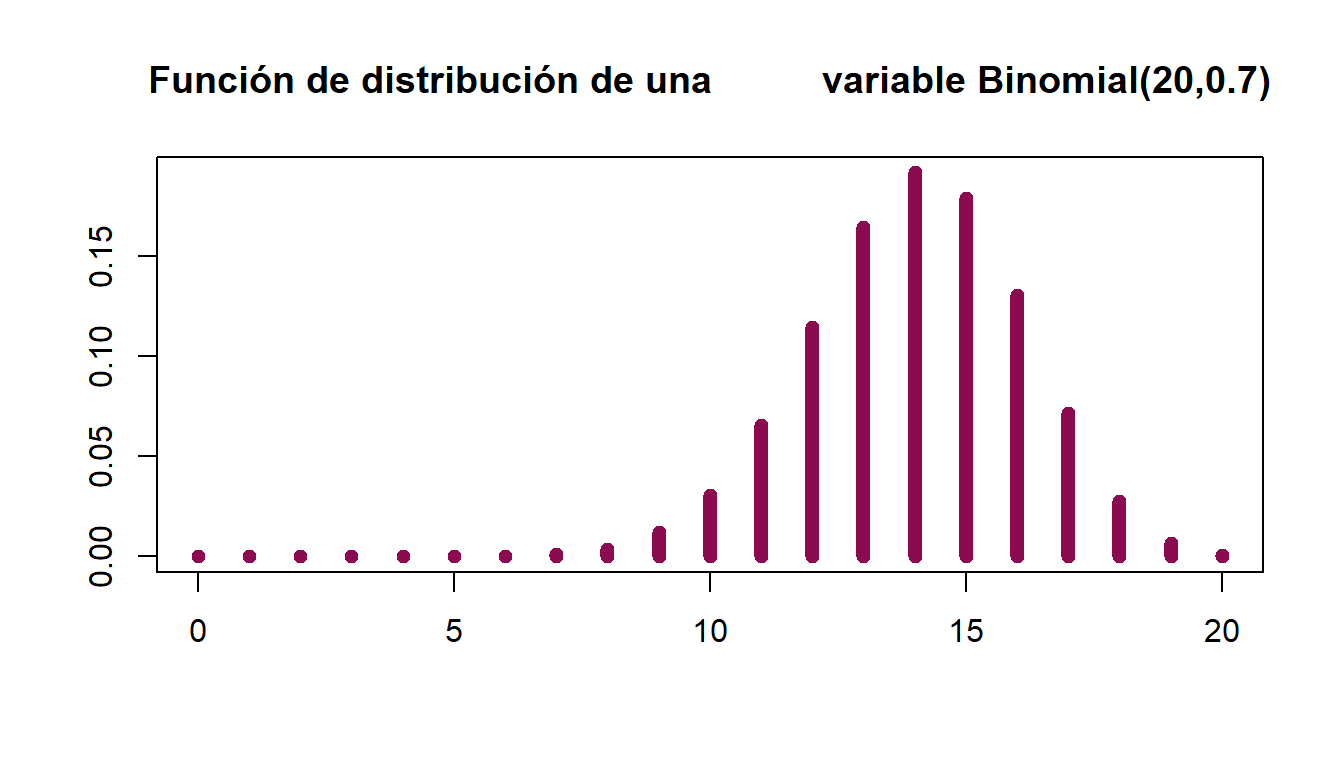
\includegraphics{_main_files/figure-latex/unnamed-chunk-4-1} \end{center}

Utilizando la función de R, debemos tener cuidado ya que nuestra muestra es pequeña:

\begin{Shaded}
\begin{Highlighting}[]
\FunctionTok{binom.test}\NormalTok{(T,n, }\AttributeTok{p =} \FloatTok{0.7}\NormalTok{, }\AttributeTok{alternative =} \FunctionTok{c}\NormalTok{(}\StringTok{"greater"}\NormalTok{))}
\end{Highlighting}
\end{Shaded}

\begin{verbatim}
    Exact binomial test

data:  T and n
number of successes = 18, number of trials = 20, p-value = 0.03548
alternative hypothesis: true probability of success is greater than 0.7
95 percent confidence interval:
 0.7173815 1.0000000
sample estimates:
probability of success 
                   0.9 
\end{verbatim}

\hypertarget{prueba-de-cuantiles}{%
\chapter{Prueba de Cuantiles}\label{prueba-de-cuantiles}}

Lo que nos interesa en ésta prueba binomial es hacer inferencia sobre los cuantiles de una variable aleatoria. Por ejemplo, muchos examinamos una muestra aleatoria de valores de alguna variable x para ver si la mediana de x es igual a 17 (por ejemplo).

La escala de medición suele ser al menos ordinal para ésta prueba de hipótesis, aunque la prueba binomial solo require la escala nominal que es más débil para su medición. Esto se debe a que los cuantiles tienen poco significado con las mediciones de escala nominal.

\textbf{Recordatorio}

El cuantil de valor \(p\) de una variable aleatoria \(X\)
es un número \(x\) tal que:

\[ \mathbf{P}[X < x]\leq p\]

\begin{itemize}
\tightlist
\item
  En el caso de una variable aleatoria continua se da la igualdad.
\end{itemize}

\hypertarget{datos-1}{%
\section{Datos}\label{datos-1}}

Los datos consisten en una muestra

\[X_{1},X_{2},X_{3},\cdots,X_{n}  \  \ \mbox{ una muestra aleatoria de tamaño} \ n \  \mbox{de la población}\]

\hypertarget{supuestos-1}{%
\section{Supuestos}\label{supuestos-1}}

\begin{enumerate}
\def\labelenumi{\arabic{enumi})}
\item
  Los datos a los que se les aplica esta prueba son una muestra aleatoria independiente e idénticamente distribuida.
\item
  La escala de medida de las \(X_{i}s\) es al menos ordinal.
\end{enumerate}

\hypertarget{estaduxedstico-de-prueba-1}{%
\section{Estadístico de Prueba}\label{estaduxedstico-de-prueba-1}}

\[T_{1}\]
El número de observaciones en la muestra que son \textbf{menores o iguales} al valor \(x^*\) sobre el que se va a hacer la hipótesis.

\[T_{2}\]
El número de observaciones en la muestra que son \textbf{estrictamente menores} a \(x^*\).

Cuando \(n\leq 20\) la distribución nula de éstos estadísticos es \(Bin(n,p=p^*)\) con \(n\) el tamaño de la muestra y \(p^*\) dada en la hipótesis nula (recuerde que queremos hacer pruebas relacionadas con el cuantil \(x_{p}\) de la \(v.a.\) en cuestión).

Por otro lado, si \(n>20\) puede resultar más sencillo utilizar una aproximación normal para realizar la prueba, en dicho caso se puede utilizar el cuantil:

\[
t=np+Z_{q}\sqrt{np(1-p)}
\]

Donde \(Z_{q}\) es el cuantil de una distribución normal estándar que se puede obtener en la tabla correspondiente.

Dependiendo del planteamiento de nuestro problema a resolver se formulan las hipótesis:

\hypertarget{hipuxf3tesis-1}{%
\section{Hipótesis}\label{hipuxf3tesis-1}}

\hypertarget{caso-a-prueba-de-dos-colas-1}{%
\subsection*{Caso A (Prueba de dos colas)}\label{caso-a-prueba-de-dos-colas-1}}


\[\textbf{H}_{o}: x_{p} = x^* \ \ \mbox{es equivalente  decir}: \ \ \mathbf{P}[X \leq x^*]= p^*\]

\[vs\]

\[\textbf{H}_a: x_{p} \neq x^* \ \ \mbox{es equivalente  decir}: \ \ \mathbf{P}[X \leq x^*]\neq p^*\]

\hypertarget{regla-de-decisiuxf3n-3}{%
\subsubsection*{Regla de decisión}\label{regla-de-decisiuxf3n-3}}


Rechazamos \(H_0\) a un nivel de significancia \(\alpha\) si

\[T_{1}\leq t_{1} \ \ \ \ \  o   \ \ \ \ \ T_{2}>t_{2}\]

Elegimos \(\alpha_{1},\alpha_{2}\geq 0\), tales que \(\alpha_{1}+\alpha_{2}=\alpha\) el tamaño de la prueba y debemos encontrar \(t_{1}\) y \(t_{2}\) tales que:

\[\mathbf{P}[Y \leq t_{1}]=\alpha_{1} \ \ \ \ \  y  \ \ \ \ \ \mathbf{P}[Y \leq t_{2}]=1-\alpha_{2}\]

Donde \(Y \sim Bin (n,p^*)\).

y calculamos el \(p-value\) de la siguiente manera:

\[p-value=2*min \{ \mathbf{P}[Y\leq T_{1}],\mathbf{P}[Y \geq T_{2}] \}\]

Sugerimos que si \(n > 20\) ,el \(p-value\) puede obtenerse usando:

\[\mathbf{P}[Y\leq T_{1}] \thickapprox \mathcal{N}\left(\frac{T_{1}-np^*+0.5}{\sqrt{np^*(1-p^*)}}\right)\]

y

\[\mathbf{P}[Y\geq T_{2}] \thickapprox 1-\mathcal{N} \left(\frac{T_{2}-np^*-0.5}{\sqrt{np^*(1-p^*)}}\right)\]
Con \(\mathcal{N}(\cdot)\) la función de distribución de la normal estándar.

\hypertarget{caso-b-prueba-de-cola-inferior-1}{%
\subsection*{Caso B (Prueba de cola inferior)}\label{caso-b-prueba-de-cola-inferior-1}}


\[\textbf{H}_0: x_{p} \leq x^* \ \ \mbox{es equivalente a decir:} \ \ \ \mathbf{P}[X < x^*]\geq p^*\]

\[vs\]

\[
\textbf{H}_a: x_{p} > x^* \ \  \mbox{es equivalente a decir}: \ \ \mathbf{P}[X < x^*]< p^*
\]

\hypertarget{regla-de-decisiuxf3n-4}{%
\subsubsection*{Regla de decisión}\label{regla-de-decisiuxf3n-4}}


Rechazamos \(H_0\) a un nivel de significancia \(\alpha\) si

\[T_{1} \leq t_{1}\]

Elegimos \(\alpha\), el tamaño de la prueba y debemos encontrar \(t_{1}\) tal que

\[\mathbf{P}[Y \leq t_{1}]=\alpha\]

Donde \(Y \sim Bin (n,p^*)\).

y calculamos el \(p-value\) de la siguiente manera:

\[p-value= \mathbf{P}[Y\leq T_{1}]\]

Sugerimos que si \(n > 20\), el \(p-value\) puede obtenerse más sencillo usando la aproximación normal:

\[\mathbf{P}[Y\leq T_{1}] \thickapprox \mathcal{N} \left(\frac{T_{1}-np^*+0.5}{\sqrt{np^*(1-p^*)}}\right)\]

\hypertarget{caso-c-prueba-de-cola-supeior}{%
\subsection*{Caso C (Prueba de cola supeior)}\label{caso-c-prueba-de-cola-supeior}}


\[\textbf{H}_0: x_{p} \geq x^* \ \ \mbox{es equivalente a decir}: \ \ \mathbf{P}[X < x^*]\leq p^*\]

\[vs\]

\[\textbf{H}_a: x_{p} < x^*  \ \ \mbox{es equivalente a decir}: \ \ \mathbf{P}[X < x^*]> p^*\]

\hypertarget{regla-de-decisiuxf3n-5}{%
\subsubsection*{Regla de decisión}\label{regla-de-decisiuxf3n-5}}


Rechazamos \(H_0\) a un nivel de significancia \(\alpha\) si

\[T_{2} > t_{2}\]

Elegimos \(\alpha\), el tamaño de la prueba y debemos encontrar \(t_{2}\) tal que

\[\mathbf{P}[Y \leq t_{2}]=1-\alpha\]~

Donde \(Y \sim Bin (n,p^*)\).

y calculamos el \(p-value\) de la siguiente manera:

\[p-value=\mathbf{P}[Y\geq T_{2}]\]

Sugerimos que si \(n > 20\) ,el \(p-value\) puede obtenerse más sencillo usando la aproximación normal:

\[\mathbf{P}[Y\geq T_{2}] \thickapprox 1- \mathcal{N} \left(\frac{T_{2}-np^*-0.5}{\sqrt{np^*(1-p^*)}}\right)\]

Ahora aplicaremos lo anterior en un ejemplo ilustrativo:

\hypertarget{ejemplo-1}{%
\section{Ejemplo}\label{ejemplo-1}}

El intervalo de tiempo entre las erupciones del geiser Old Faithful se registra 112 veces, de las cuales 8 son menores a 60 minutos y una es exactamente 60 minutos. Se quiere desea verificar que la mediana del intervalo es mayor a 60 minutos.

\textbf{Paso 1} Escribimos la prueba a utilizar

La prueba a utilizar \textbf{Prueba de cuantiles caso B cola inferior}

\textbf{Paso 2} Formulamos nuestras hipótesis en contexto al problema planteado

\[\textbf{H}_0: \mathbf{P}[X \leq 60]\geq 0.50\]

\[vs\]

\[\textbf{H}_a:  \mathbf{P}[X \leq 60]<0.50\]

Donde \(X\) es el intervalo de tiempo entre las erupciones, asumiendo que ambos intervalos son independientes e identicamente distribuidas.

\textbf{Paso 3} Estadístico de prueba

La estadística de prueba será \(T_1=9\) y \(T_2=8\). Tomaremos \(\alpha=.1\)

\[T_{1}=9 \ \mbox{número  de  intervalos que  son menores o iguales  a 60 minutos.}\]

\[T_{2}=8 \ \mbox{número  de  intervalos que  son estrictamente menores a 60 minutos.}\]

\[T_{1}\sim Bin(112,0.50)\]

\textbf{Paso 4} Procedimiento completo

\textbf{Supuestos:}

\begin{enumerate}
\def\labelenumi{\arabic{enumi}.}
\tightlist
\item
  Muestra aleatoria de tamaño 112.
\end{enumerate}

\begin{itemize}
\item
  Tomaremos \(\alpha = 5% = 0.05
  \) el nivel de significancia.
\item
  \(n = 112\) tamaño de la muestra
\item
  \(p^* = 0.50\)
\end{itemize}

\textbf{Paso 5} Regla de decisión

Rechazamos \(H_0\) a un nivel de significancia \(\alpha\) si \(T_{1} \leq t_{1}\) y Rechazo \(H_0\) si \(p-value<\alpha\)

\[T_{1}=9 \leq 47.3=t_{1}\]

como \(n>20\) puede resultar más sencillo utilizar una aproximación normal para realizar la prueba, en dicho caso se puede utilizar el estadístico:

\[t_{1}=np+Z_{q}\sqrt{np(1-p)}=(112)(0.5)+(-1.645)\sqrt{112(0.5)(1-0.5)}\]

\[t_{1}=47.3\]

\(\therefore\) Rechazamos \(H_0\)

y calculamos el \(p-value\) de la siguiente manera:

\[p-value= \mathbf{P}[Y\leq T_{1}]=\mathbf{P}[Y\leq 9]\]

Como \(n > 20\), el \(p-value\) puede obtenerse más sencillo usando la aproximación normal:

\[\mathbf{P}[Y\leq 9] \thickapprox \mathcal{P} \left[Z\leq\frac{T_{1}-np^*+0.5}{\sqrt{np^*(1-p^*)}}\right]=\]
\[\left(Z\leq\frac{9-(112)(0.5)+0.5}{\sqrt{(112)(0.5)(1-0.5)}}\right)=\mathbf{P}[Z\leq -8.7876] < < 0.0001\]
\(\therefore\) Rechazo \(H_0\) ya que \(p-value=0.0001<<0.05=\alpha.\) es decir, el \(p-value\) es ``muy pequeño''.

\textbf{Paso 6} Conclusión

Existe información suficiente para decir que la mediana del intervalo de erupciones es mayor a 60 minutos.

\hypertarget{ejemplo-en-r-studio-1}{%
\section{Ejemplo en R-Studio}\label{ejemplo-en-r-studio-1}}

Ahora haremos la réplica en R.

La estadística de prueba será \(T_1=9\) y \(T_2=8\). Tomaremos \(\alpha=.1\)

\begin{Shaded}
\begin{Highlighting}[]
\CommentTok{\#Datos}

\NormalTok{T\_1}\OtherTok{=}\DecValTok{9}         \CommentTok{\#Observaciones menores/iguales a 60 minutos}
\NormalTok{T\_2}\OtherTok{=}\DecValTok{8}         \CommentTok{\#Observaciones que son menores estrictamente a 60 minutos}
\NormalTok{alpha}\OtherTok{=}\FloatTok{0.05}    \CommentTok{\#Nivel de significancia}
\NormalTok{n}\OtherTok{=}\DecValTok{112}         \CommentTok{\#Tamaño de la muestra}
\NormalTok{p}\OtherTok{=}\FloatTok{0.5}         \CommentTok{\#Cuantil en este caso la mediana }
\end{Highlighting}
\end{Shaded}

Según el planteamiento de las hipótesis, este es un Caso B (de cola inferior), por lo que siguiendo la regla de decisión, se rechaza \(H_0\) si \(T_1\leq t_1\) donde \(t_1\) será el cuantil que acumule 10\% en la distribución binomial

Podemos graficar la función de distribución:

\begin{center}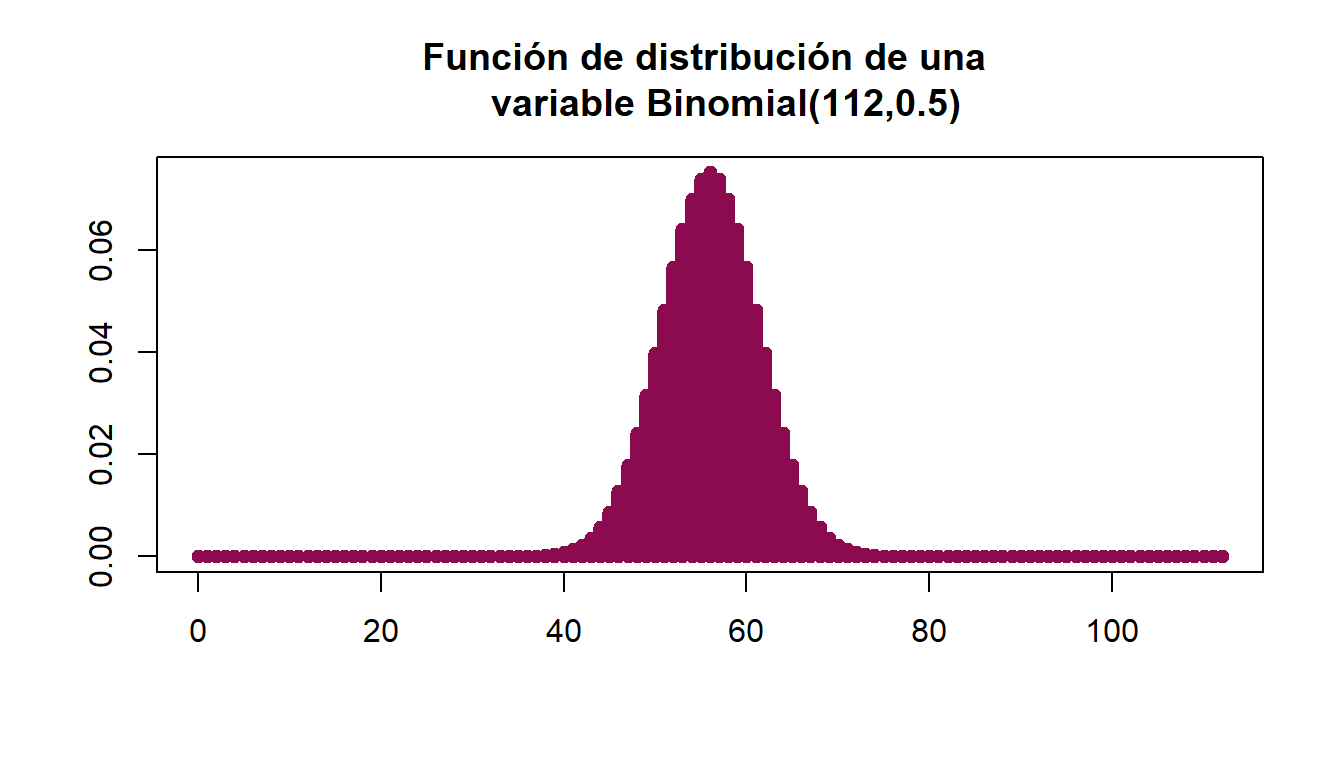
\includegraphics{_main_files/figure-latex/unnamed-chunk-7-1} \end{center}

A continuación calculamos \(t_1\) y el \(p-value\):

\begin{Shaded}
\begin{Highlighting}[]
\NormalTok{t\_1}\OtherTok{=}\FunctionTok{qbinom}\NormalTok{(.}\DecValTok{10}\NormalTok{,n,p)        }\CommentTok{\#Cuantil a comparar con el estadístico de prueba}
\NormalTok{t\_1}
\end{Highlighting}
\end{Shaded}

\begin{verbatim}
[1] 49
\end{verbatim}

\begin{Shaded}
\begin{Highlighting}[]
\NormalTok{pvalue}\OtherTok{=}\FunctionTok{pbinom}\NormalTok{(T\_1,n,p)     }\CommentTok{\#P{-}value correspondiente}
\NormalTok{pvalue}
\end{Highlighting}
\end{Shaded}

\begin{verbatim}
[1] 1.157256e-21
\end{verbatim}

Tenemos que como \(T_1=9\leq 49 =t_1\), entonces se rechaza \(H_0\) y por lo tanto se concluye que hay información suficiente para decir que la mediana de los intervalos de tiempo entre erupciones es mayor a 60 minutos.

Al mismo resultado llegamos si en lugar de buscar \(t_1\) calculamos el \(p-value\) de la estadística \(T_1\) la cual da un valor muy cercano a cero por lo tanto cae en la región de rechazo y se conlcuye que la mediana de los intervalos de tiempo entre erupciones es mayor a 60 minutos.

Finalmente podemos utilizar la función en R.

\begin{Shaded}
\begin{Highlighting}[]
\FunctionTok{binom.test}\NormalTok{(T\_1,n,}\AttributeTok{p=}\FloatTok{0.5}\NormalTok{,}\AttributeTok{alternative =} \StringTok{"less"}\NormalTok{)}
\end{Highlighting}
\end{Shaded}

\begin{verbatim}
    Exact binomial test

data:  T_1 and n
number of successes = 9, number of trials = 112, p-value < 2.2e-16
alternative hypothesis: true probability of success is less than 0.5
95 percent confidence interval:
 0.000000 0.136034
sample estimates:
probability of success 
            0.08035714 
\end{verbatim}

\hypertarget{prueba-de-signos}{%
\chapter{Prueba de Signos}\label{prueba-de-signos}}

La prueba de signos merece una consideración especial debido a su versatilidad, su gran utilidad y simplicidad. Ésta es una prueba de proporciones cuando el valor específico \(p^*=1/2\) y para los casos de dos colas, cola inferior y cola superior la máxima probabilidad para rechazar la hipótesis nula \(H_0\) se da cuando \(p = 1/2\). Frecuentemente la prueba de signos también es apropiada para analizar datos de un vector aleatorio \((X,Y)\) y ver si alguna de sus entradas tiene valores más grandes que la otra. De esta manera, si una variable tiende a tener valores mayores que la otra, se puede utilizar la prueba de signos para determinar si las medias de éstas variables son diferentes.

\hypertarget{datos-2}{%
\section{Datos}\label{datos-2}}

Los datos consisten en observaciones bivariadas aleatorias:

\[(X_{1},Y_{1}),(X_{2},Y_{2}),(X_{3},Y_{3}),\cdots,(X_{n'},Y_{n'})\]

Dentro de cada par de datos en la muestra se clasificará de la siguiente manera:

\begin{itemize}
\tightlist
\item
  Por un signo \("+"\) cuando \(X_{i} < Y_{i}\)
\item
  Por un signo ``-'' cuando \(X_{i} > Y_{i}\)
\item
  Se omitirán las parejas cuando \(Xi = Yi\).
\end{itemize}

El tamaño de la muestra después de quitar los empates será \(n\).

\hypertarget{supuestos-2}{%
\section{Supuestos}\label{supuestos-2}}

\begin{enumerate}
\def\labelenumi{\arabic{enumi})}
\item
  Las variables aleatorias bivariadas \((X_{i},Y_{i})\) son mutuamente independientes.
\item
  La escala de medida es al menos ordinal dentro de cada par.
\end{enumerate}

\hypertarget{estaduxedstico-de-prueba-2}{%
\section{Estadístico de Prueba}\label{estaduxedstico-de-prueba-2}}

\[T=Total\ de\ signos\ "+"\]

La distribución nula de \(T\) es una distribución binomial con \(n\) el número de parejas de la muestra sin empates y \(p=1/2\).

\[T\sim Bin(n,1/2)\]

Dependiendo del planteamiento de nuestro problema a resolver se formulan las hipótesis:

\hypertarget{hipuxf3tesis-2}{%
\section{Hipótesis}\label{hipuxf3tesis-2}}

\hypertarget{caso-a-prueba-de-dos-colas-2}{%
\subsection*{Caso A (Prueba de dos colas)}\label{caso-a-prueba-de-dos-colas-2}}


\[\textbf{H}_0: \mathbf{P}[obtener\ +]= \mathbf{P}[obtener\ -]\]

\[vs\]

\[\textbf{H}_a: \mathbf{P}[obtener\ +] \neq \mathbf{P}[obtener\ -]\]

\hypertarget{regla-de-decisiuxf3n-6}{%
\subsubsection*{Regla de decisión}\label{regla-de-decisiuxf3n-6}}


Rechazamos \(H_0\) a un nivel de significancia \(\alpha\) si

\[T \leq t \ \ \  o \ \ \ T>n-t\]

Elegimos \(\alpha\), el tamaño de la prueba y debemos encontrar \(t\) tal que

\[\mathbf{P}[Y \leq t]=\alpha/2\]

Donde \(Y \sim Bin (n,1/2)\).

Por otro lado, si \(n>20\) puede resultar más sencillo utilizar una aproximación normal para realizar la prueba, en dicho caso se puede utilizar el siguiente cuantil:

\[t=\frac{1}{2}\left(n+z_{\alpha/2}\ \sqrt{n}\right)\]

Donde \(z_{\alpha/2}\) es el cuantil de una distribución normal estándar que se puede obtener en la tabla correspondiente.

y calculamos el \(p-value\) de la siguiente manera:

\[p-value=2*min\{\mathbf{P}[Y\leq T],\mathbf{P}[Y\geq T]\}\]

Sugerimos que si \(n > 20\), el \(p-value\) puede obtenerse más sencillo usando la aproximación normal:

\[\mathbf{P}[Y\leq T] \thickapprox  \mathcal{N}\left(\frac{2T-n+1}{\sqrt{n}}\right)\]
\[\mathbf{P}[Y\geq T] \thickapprox 1- \mathcal{N} \left(\frac{2T-n-1}{\sqrt{n}}\right)\]

\hypertarget{caso-b-prueba-de-cola-inferior-2}{%
\subsection*{Caso B (Prueba de cola inferior)}\label{caso-b-prueba-de-cola-inferior-2}}


\[\textbf{H}_0: \mathbf{P}[obtener\ +] \geq \mathbf{P}[obtener\ -]\]

\[vs\]

\[\textbf{H}_a: \mathbf{P}[obtener\ +] < \mathbf{P}[obtener\ -]\]

\hypertarget{regla-de-decisiuxf3n-7}{%
\subsubsection*{Regla de decisión}\label{regla-de-decisiuxf3n-7}}


Rechazamos \(H_0\) a un nivel de significancia \(\alpha\) si

\[T \leq t\]

Elegimos \(\alpha\), el tamaño de la prueba y debemos encontrar \(t\) tal que:

\[\mathbf{P}[Y \leq t]=\alpha\]

Donde \(Y \sim Bin (n,1/2)\).

y calculamos el \(p-value\) de la siguiente manera:

\[p-value=\mathbf{P}[Y\leq T]\]

Sugerimos que si \(n > 20\),el \(p-value\) puede obtenerse más sencillo usando la aproximación normal:

\[\mathbf{P}[Y\leq T] \thickapprox  \mathcal{N} \left(\frac{2T-n+1}{\sqrt{n}}\right)\]

\hypertarget{caso-c-prueba-de-cola-superior-1}{%
\subsection*{Caso C (Prueba de cola superior)}\label{caso-c-prueba-de-cola-superior-1}}


\[\textbf{H}_0: \mathbf{P}[obtener\ +] \leq \mathbf{P}[obtener\ -]\]

\[vs\]

\[\textbf{H}_a: \mathbf{P}[obtener\ +] > \mathbf{P}[obtener\ -]\]

\hypertarget{regla-de-decisiuxf3n-8}{%
\subsubsection*{Regla de decisión}\label{regla-de-decisiuxf3n-8}}


Rechazamos \(H_0\) a un nivel de significancia \(\alpha\) si

\[T > n-t\]

Elegimos \(\alpha\), el tamaño de la prueba y debemos encontrar \(t\) tal que

\[\mathbf{P}[Y \leq t]=\alpha\]

Donde \(Y \sim Bin (n,1/2)\).

y calculamos el \(p-value\) de la siguiente manera:

\[p-value=\mathbf{P}[Y\geq T]\]

Sugerimos que si \(n > 20\), el \(p-value\) puede obtenerse más sencillo usando la aproximación normal:

\[\mathbf{P}[Y\geq T] \thickapprox 1- \mathcal{N} \left(\frac{2T-n-1}{\sqrt{n}}\right)\]

Ahora aplicaremos lo anterior en un ejemplo ilustrativo:

\hypertarget{ejemplo-2}{%
\section{Ejemplo}\label{ejemplo-2}}

Un grupo de 6 amigos se puso a dieta, en un intento para perder peso obtuvieron los siguientes resultados:

\[
\begin{array}{c c c c } 
\textbf{Nombre} & \textbf{Peso Antes} & \textbf{Peso Después} \\
\hline
Ed    & 174 & 165 \\
Jim   & 191 & 186 \\
Max   & 188 & 183 \\
Ray   & 182 & 178 \\
Abdul & 201 & 203 \\
Phil  & 188 & 181 \\
\end{array} 
\]

El grupo de amigos desea ver si la dieta que están realizando es efectiva.

Recordando que cada par de datos en la muestra se clasificará de la siguiente manera:

\begin{itemize}
\tightlist
\item
  \("+"\) cuando \(X_{i} < Y_{i}\)
\item
  \("-"\) cuando \(X_{i} > Y_{i}\)
\end{itemize}

y se omitirán las parejas cuando \(X_i = Y_i\). Y el tamaño de la muestra después de quitar los empates será \(n\), haremos lo siguiente:

\[
\begin{array}{|c |c |c |c c c|}
\hline
\textbf{Nombre} & \textbf{Peso Antes} & \textbf{Peso Después} & \textbf{Signo} \\
 & \textbf{X}_i & \textbf{Y}_i & \\
 \hline
Ed    & 174 & 165  &  "-"   \\
Jim   & 191 & 186  &  "-" \\
Max   & 188 & 183  &  "-" \\
Ray   & 182 & 178  &  "-" \\
Abdul & 201 & 203  &  "+" \\
Phil  & 188 & 181  &  "-"  \\
\hline
\end{array} 
\]

\textbf{Paso 1} Escribimos la prueba a utilizar

La prueba a utilizar \textbf{Prueba de signos Caso B cola inferior}

\textbf{Paso 2} Formulamos nuestras hipótesis en contexto al problema planteado

\[\textbf{H}_0: \mathbf{P}[obtener\ +] \geq \mathbf{P}[obtener\ -]\]

\[vs\]

\[\textbf{H}_a: \mathbf{P}[obtener\ +] < \mathbf{P}[obtener\ -]\]

es decir,

\[\textbf{H}_0: \mbox{En promedio los pesos antes de la dieta son mayores a los pesos después de la dieta.}\]

\[vs\]

\[\textbf{H}_a:\mbox{ En promedio los pesos después de las dieta son mayores a los pesos antes de la dieta.}\]

\textbf{Paso 3} Estadístico de prueba

Utilizaremos el estadístico

\[T=1 \ \ número \ de \ signos\ "+"\]

\[T\sim Bin(6,1/2)\]

\textbf{Paso 4} Procedimiento completo

\textbf{Supuestos:}

\begin{enumerate}
\def\labelenumi{\arabic{enumi}.}
\tightlist
\item
  Muestra aleatoria de tamaño 6.
\end{enumerate}

\begin{itemize}
\item
  Tomaremos como ``éxito'' los que si perdieron peso, en este caso los signos ``+''
\item
  Tomaremos \(\alpha\)= 5\% =0.05 el nivel de significancia.
\item
  \(n=6\) tamaño de la muestra
\item
  \(p\)=1/2
\end{itemize}

\textbf{Paso 5} Regla de decisión

Rechazamos \(H_0\) a un nivel de significancia \(\alpha\) si \(T \leq t\)

\[T=1 \leq 1=t\]

\(\therefore\) Rechazamos \(H_0\)

y calculamos el \(p-value\) de la siguiente manera:

\[p-value=\mathbf{P}[Y\leq T]=\mathbf{P}[Y\leq 1]=0.1093\]

\(\therefore\) \(p-value=0.1093>0.05=\alpha\) entonces no rechazamos \(H_0\).

Nos preguntaremos, ¿Cómo es que pasa esto?, bueno esto se debe a que nuestra muestra es muy pequeña (son 6 datos), claro no siempre vamos a tener muestras así. Pero, debemos tener en cuenta que al tener muestras reducidas le estamos reduciendo potencia a la prueba de hipótesis utilizada, ya que la capacidad de detectar diferencias significativas entre los datos disminuye.

\textbf{Paso 6} Conclusión

Existe evidencia suficiente para decir que los pesos después de la dieta son menores a los pesos antes de la dieta.

\hypertarget{ejemplo-en-r-studio-2}{%
\section{Ejemplo en R-Studio}\label{ejemplo-en-r-studio-2}}

Ahora haremos la réplica en R.

La estadística de prueba será \(T=1\). Tomaremos \(\alpha=5\%\)

\begin{Shaded}
\begin{Highlighting}[]
\CommentTok{\#Datos}

\NormalTok{T}\OtherTok{=}\DecValTok{1}              \CommentTok{\#Número de éxitos (+)}
\NormalTok{alpha}\OtherTok{=}\FloatTok{0.05}       \CommentTok{\#Nivel de }
\NormalTok{n}\OtherTok{=}\DecValTok{6}              \CommentTok{\#Tamaño de la muestra }
\NormalTok{p}\OtherTok{=}\FloatTok{0.5}            \CommentTok{\#Para la prueba de signos "p" siempre será 1/2}
\end{Highlighting}
\end{Shaded}

Según el planteamiento de las hipótesis, este es un Caso B (de cola inferior), por lo que siguiendo la regla de decisión, se rechazará \(H_0\) si \(T\leq t\) donde \(t\) será en cuantil que acumule 5\% en la distribución binomial

Podemos graficar la función de distribución:

\begin{center}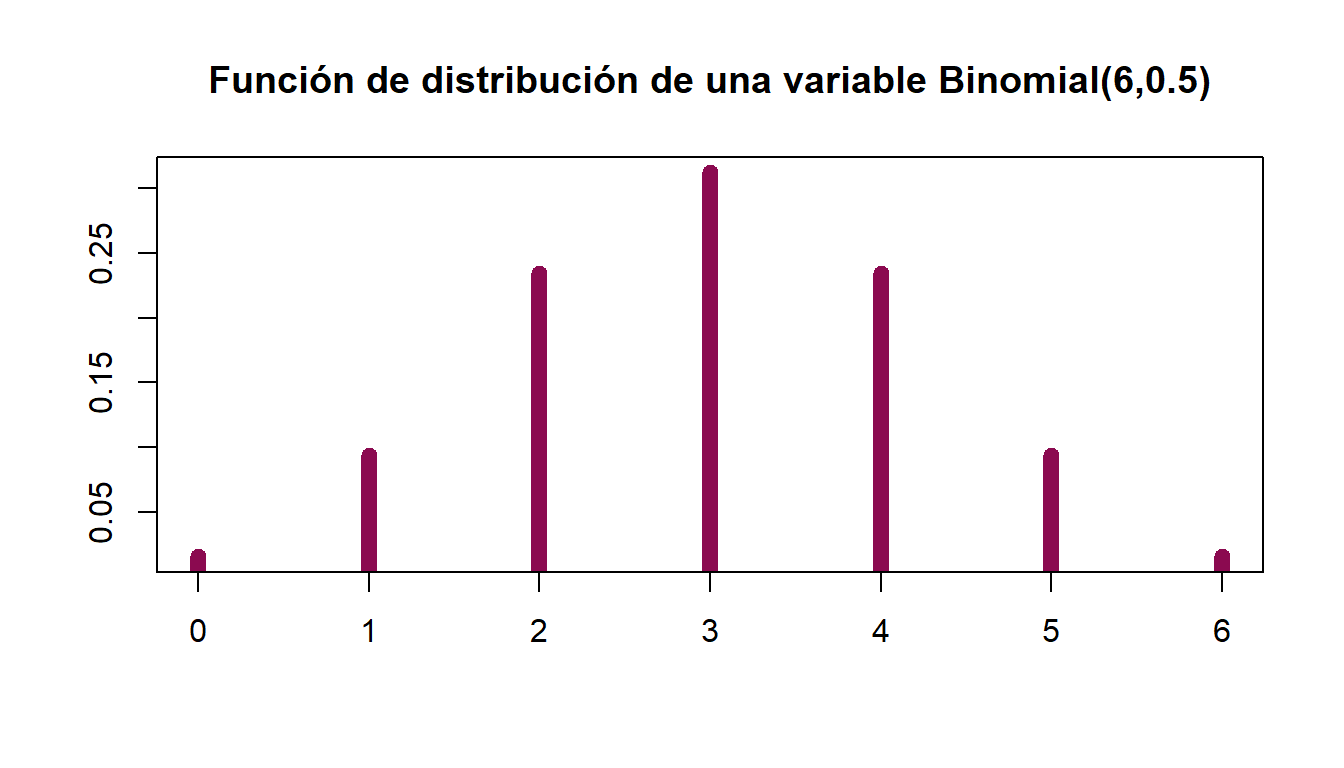
\includegraphics{_main_files/figure-latex/unnamed-chunk-11-1} \end{center}

Calculamos t y el \(p-value\):

\begin{Shaded}
\begin{Highlighting}[]
\NormalTok{t}\OtherTok{=}\FunctionTok{qbinom}\NormalTok{(.}\DecValTok{05}\NormalTok{,n,p)         }\CommentTok{\#Valor a comparar con nuestro estadístico}
\NormalTok{t}
\end{Highlighting}
\end{Shaded}

\begin{verbatim}
[1] 1
\end{verbatim}

\begin{Shaded}
\begin{Highlighting}[]
\NormalTok{pvalue}\OtherTok{=}\FunctionTok{pbinom}\NormalTok{(T,n,p)       }\CommentTok{\#P{-}value}
\NormalTok{pvalue}
\end{Highlighting}
\end{Shaded}

\begin{verbatim}
[1] 0.109375
\end{verbatim}

Tenemos que como \(T=1\leq 1 =t\), entonces se rechaza \(H_0\) y por lo tanto se concluye que hay información suficiente para decir que en promedio los pesos después de la dieta son menores a los pesos antes de la dieta. Por lo tanto la dieta parece funcionar.

Finalmente utilizaremos la función de R:

\begin{Shaded}
\begin{Highlighting}[]
\FunctionTok{binom.test}\NormalTok{(T,n,}\AttributeTok{p=}\FloatTok{0.5}\NormalTok{,}\AttributeTok{alternative =} \StringTok{"less"}\NormalTok{)}
\end{Highlighting}
\end{Shaded}

\begin{verbatim}
    Exact binomial test

data:  T and n
number of successes = 1, number of trials = 6, p-value = 0.1094
alternative hypothesis: true probability of success is less than 0.5
95 percent confidence interval:
 0.0000000 0.5818034
sample estimates:
probability of success 
             0.1666667 
\end{verbatim}

\hypertarget{prueba-mc-nemar}{%
\chapter{Prueba Mc Nemar}\label{prueba-mc-nemar}}

El objetivo de esta prueba es ver el efecto que tuvo cierto ``tratamiento'' sobre un sujeto cuya ``condición'' se observa antes y después del mismo.
Por ejemplo se puede usar para analizar el efecto que un debate tiene en la decisión de una asamblea. Para esto se puede hacer una encuesta para registrar la opinión de los miembros de la misma en categorías \textbf{a favor} o \textbf{en contra} de una propuesta y después de realizado el debate se les vuelve a preguntar su opinión sobre el tema.
Nos interesa estudiar a los individuos que cambiaron de opinión, es decir, los que antes estaban \textbf{a favor} y ahora están \textbf{en contra} y los que estaban \textbf{en contra} y ahora están \textbf{a favor}.

La manera de estudiar esto es identificando a los individuos encuestados con parejas ordenadas de la forma (0,0),(0,1),(1,0) o (1,1) dónde la primera entrada representa la \textbf{postura} del individuo
antes del debate y la segunda representa su postura después. (``0'',por ejemplo, puede representar \textbf{en contra} y ``1'' \textbf{a favor}).
Luego se ingresan estos datos en una tabla de contingencia de la siguiente forma:

\[
\begin{array}{ c| c| c }
 & \textbf{ahora en contra}  & \textbf{ahora a favor}\\
\hline
\textbf{antes en contra} & Número\ de\ (0,0) & Número\ de\ (0,1) \\
\hline
\textbf{antes a favor} & Número\ de\ (1,0) & Número\ de\ (1,1) \\
\end{array} 
\]

\hypertarget{datos-3}{%
\section{Datos}\label{datos-3}}

Los datos consisten en observaciones bivariadas aleatorias:

\[(X_{1},Y_{1}),(X_{2},Y_{2}),(X_{3},Y_{3}),\cdots,(X_{n'},Y_{n'})\]

Dentro de cada par de datos en la muestra se tiene \(X\) e \(Y\) que sólo tomarán los valor \(0\) y \(1\).

En general los datos se resumen en una tabla de contingencia de la forma:

\[
\begin{array}{ c| c| c }
 & \textbf{después 0}  & \textbf{después 1}\\
\hline
\textbf{antes 0} & \textbf{a}=Número\ de\ (0,0) &\textbf{b}=Número\ de\ (0,1) \\
\hline
\textbf{antes 1} & \textbf{c}=Número\ de\ (1,0) &\textbf{d}=Número\ de\ (1,1) \\
\end{array} 
\]

\hypertarget{supuestos-3}{%
\section{Supuestos}\label{supuestos-3}}

\begin{enumerate}
\def\labelenumi{\arabic{enumi})}
\item
  Cada pareja (\(X_{i},Y_{i}\)) son mutuamente independientes.
\item
  La escala de medida es nominal con 2 categorías para toda \(X_{i}\) y \(Y_{i}\).
\item
  La probabilidad de que se observe (0,1) es \(\geq\) que la de (1,0) o la de (1,0) es \(\geq\) (0,1) para todos los elementos de la muestra.
\end{enumerate}

\hypertarget{estaduxedstico-de-prueba-3}{%
\section{Estadístico de Prueba}\label{estaduxedstico-de-prueba-3}}

\[T_{1}=\frac{(b-c)^2}{(b+c)} \ \thickapprox \ \chi^{2}_{(1)}\]
Es decir, la distribución de \(T_{1}\) es aproximadamente \(\chi^{2}_{(1)}\).

Por otro lado, si \(b+c\leq20\), es preferible utilizar el siguiente estadístico:

\[T_{2}=b\sim Bin(b+c,p)\]

Es decir, la distribución de \(T_{2}\) es exactamente \(Bin(b+c,p)\)

Dependiendo del planteamiento de nuestro problema a resolver se formulan las hipótesis:

\hypertarget{hipuxf3tesis-3}{%
\section{Hipótesis}\label{hipuxf3tesis-3}}

\hypertarget{caso-a-prueba-de-dos-colas-3}{%
\subsection*{Caso A (Prueba de dos colas)}\label{caso-a-prueba-de-dos-colas-3}}


\[\textbf{H}_0: \mathbf{P}[X_{i}=0,Y_{i}=1]= \mathbf{P}[X_{i}=1,Y_{i}=0]\]
\[vs\]

\[\textbf{H}_a: \mathbf{P}[X_{i}=0,Y_{i}=1]\neq \mathbf{P}[X_{i}=1,Y_{i}=0]\]

Es decir, se quiere ver si la probabilidad de que el individuo pase de 0 a 1 es la misma que la probabilidad de que pase de 1 a 0. En otras palabras, se quiere comprobar si el efecto del tratamiento fue neutro o si hay alguna tendencia tras el mismo.

\hypertarget{regla-de-decisiuxf3n-9}{%
\subsubsection*{Regla de decisión}\label{regla-de-decisiuxf3n-9}}


Rechazamos \(H_0\) a un nivel de significancia \(\alpha\) si

\[T_{2} \leq t \ \ \   o \ \ \ T_{2}>n-t\]

Elegimos \(\alpha\), el tamaño de la prueba y debemos encontrar \(t\) tal que

\[\mathbf{P}[Y \leq t]=\alpha/2\]

Donde \(Y \sim Bin (b+c,1/2)\).

Por otro lado, si \(b+c>20\)

Rechazamos \(H_0\) a un nivel de significancia \(\alpha\) si

\[T_{1} > t_{1-\alpha}\]

Elegimos \(\alpha\), el tamaño de la prueba y debemos encontrar \(t_{1-\alpha}\) tal que

Donde \(t_{1-\alpha}\) se encuentra en la tabla correspondiente ya que \(T_{1} \sim \chi^{2}_{(1)}\).

y calculamos el \(p-value\) de la siguiente manera:

\[p-value=2*min\{\mathbf{P}[Y\leq T_{2}],\mathbf{P}[Y\geq T_{2}]\}\]

Ahora aplicaremos lo anterior en un ejemplo ilustrativo:

\hypertarget{ejemplo-3}{%
\section{Ejemplo}\label{ejemplo-3}}

May y Johnson (1997) publicaron el resultado de un estudio en el cual los investigadores querían determinar el efecto de la hipnosis en reducir el dolor asociado con la venopunción en pacientes juveniles de cáncer. Los datos se observan en la siguiente tabla:

\[
\begin{array}{ c| c c| c }
                     & Después\ de\ la\ hipnosis &            & \\
\hline
Antes\ de\ la hipnosis & \textbf{Sin Dolor}     & \textbf{Con Dolor}& Total\\
\hline
\textbf{Sin Dolor} & \textbf{a}=18                     & \textbf{b}=4  & 22   \\
\hline
\textbf{Con Dolor} & \textbf{c}=12                     & \textbf{d}=5 & 17\\
\hline
Total     & 30              & 9               & 39 \\
\end{array} 
\]

\textbf{Paso 1} Escribimos la prueba a utilizar

La prueba a utilizar \textbf{Prueba de Mc Nemar Caso A de dos colas}

\textbf{Paso 2} Formulamos nuestras hipótesis en contexto al problema planteado

\[\textbf{H}_0: \mathbf{P}[X_{i}=0,Y_{i}=1]= \mathbf{P}[X_{i}=1,Y_{i}=0]\]

\[vs\]

\[\textbf{H}_a: \mathbf{P}[X_{i}=0,Y_{i}=1]\neq \mathbf{P}[X_{i}=1,Y_{i}=0]\]

es decir,

\[\textbf{H}_0: \ \mbox{Se mantiene el sentir dolor después de la hipnosis.}\]

\[vs\]

\[\textbf{H}_a:\ \mbox{Hay un cambio considerable al no sentir dolor después de la hipnosis.}\]

\textbf{Paso 3} Estadístico de prueba

Recordando que \(b+c=4+12\) entonces \(b+c=16\leq20\) entonces utilizaremos el estadístico:

\[T_{2}=b=4\]
\[T_{2}\sim Bin(16,1/2)\]

\textbf{Paso 4} Procedimiento completo

\textbf{Supuestos}

\begin{enumerate}
\def\labelenumi{\arabic{enumi}.}
\tightlist
\item
  Muestra aleatoria de tamaño n=16.
\end{enumerate}

\begin{itemize}
\item
  Tomaremos \(\alpha\)= 5\% =0.05 el nivel de significancia.
\item
  \(n=6\) tamaño de la muestra
\item
  \(p\)=1/2
\end{itemize}

\textbf{Paso 5} Regla de decisión

Rechazamos \(H_0\) a un nivel de significancia \(\alpha\) si \(T_{2} \leq t\) o \(T_{2}>n-t\)

Debemos encontrar \(t\) tal que

\[\mathbf{P}[Y \leq t]=\alpha/2=0.025\]

\[T_{2}=4 \leq 5=t  \ \ \ \ \   o  \ \ \ \ \      5>16-4  \]
\[T_{2}=4 \nleq 5=t   \ \ \ \ \   y   \ \ \ \ \      5\ngtr12\]

\(\therefore\) Rechazamos \(H_0\)

\textbf{Paso 6} Conclusión

Existe evidencia suficiente para decir que hay un cambio considerable a no sentir dolor después de recibir hipnosis.

\hypertarget{ejemplo-en-r-studio-3}{%
\section{Ejemplo en R-Studio}\label{ejemplo-en-r-studio-3}}

Ahora haremos la réplica en R.

Veamos que \(b+c=4+12=16\leq 20\) por lo tanto el estadístico de prueba será

\(T_2=b=4\)
\(T_2\sim Bin(16,1/2)\)

Tomaremos \(\alpha=5\%\)

\begin{verbatim}
              Despues hipnosis
Antes hipnosis Sin dolor dolor
     Sin dolor        18     4
     dolor            12     5
\end{verbatim}

\begin{Shaded}
\begin{Highlighting}[]
\CommentTok{\#Datos}

\NormalTok{T\_2}\OtherTok{=}\DecValTok{4}                    \CommentTok{\#Es la posición b}
\NormalTok{n}\OtherTok{=}\DecValTok{16}                     \CommentTok{\#Tamaño de la muestra}
\NormalTok{alpha}\OtherTok{=}\FloatTok{0.05}               \CommentTok{\#Nivel de significancia}
\NormalTok{p}\OtherTok{=}\FloatTok{0.5}                    \CommentTok{\#Para la prueba Mc nemar p es 1/2}
\end{Highlighting}
\end{Shaded}

Según el planteamiento de las hipótesis, este es un Caso A (dos colas), por lo que siguiendo la regla de decisión tenemos que rechazaremos \(H_0\) si \(T_2 \leq t\) o \(T_2>n-t\) donde \(t\) será en cuantil que acumule 5\% en la distribución binomial

Podemos graficar la función de distribución:

\begin{center}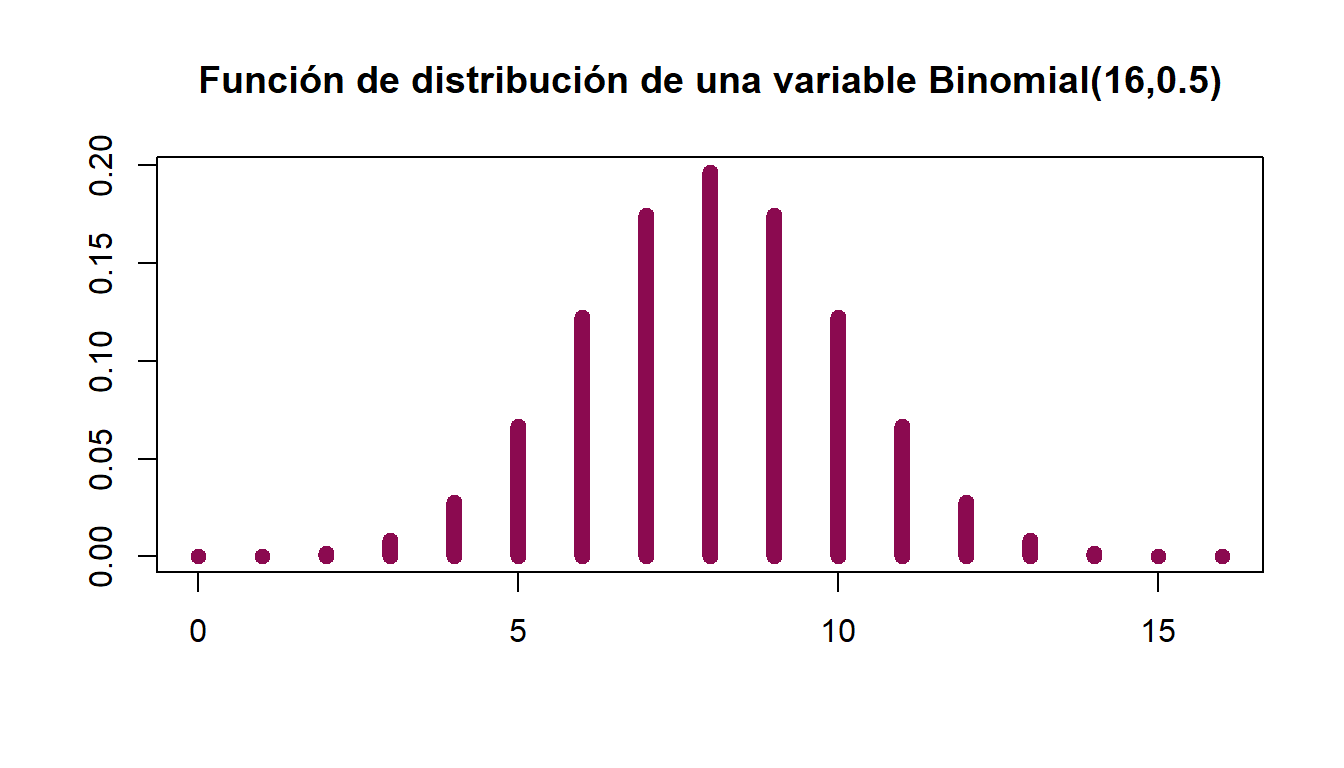
\includegraphics{_main_files/figure-latex/unnamed-chunk-16-1} \end{center}

Calculamos \(t\) y el \(p-value\):

\begin{Shaded}
\begin{Highlighting}[]
\NormalTok{t}\OtherTok{=}\FunctionTok{qbinom}\NormalTok{(.}\DecValTok{05}\NormalTok{,n,p)       }\CommentTok{\#Valor con el que vamos a comparar el estadístico}
\NormalTok{t}
\end{Highlighting}
\end{Shaded}

\begin{verbatim}
[1] 5
\end{verbatim}

\begin{Shaded}
\begin{Highlighting}[]
\NormalTok{pvalue}\OtherTok{=}\DecValTok{2}\SpecialCharTok{*}\FunctionTok{min}\NormalTok{(}\FunctionTok{c}\NormalTok{(}\FunctionTok{pbinom}\NormalTok{(T\_2,n,p), }\FunctionTok{pbinom}\NormalTok{(T\_2,n,p,}\AttributeTok{lower.tail =}\NormalTok{ F)))   }\CommentTok{\#P{-}value}
\NormalTok{pvalue}
\end{Highlighting}
\end{Shaded}

\begin{verbatim}
[1] 0.07681274
\end{verbatim}

Tenemos que como \(T_2=4\leq 5 =t\), entonces se rechaza \(H_0\) como ya rechazamos en la cola inferior no es necesario probar la cola superior, pero si NO hubieramos rechazado con la primer ecuación debemos probar si \(T_2>n-t\).

Por lo tanto se concluye que hay información suficiente para decir que hay un cambio considerable al no sentir dolor después de la hipnosis.

Finalmente utilizaremos la función en R:

\begin{Shaded}
\begin{Highlighting}[]
\FunctionTok{binom.test}\NormalTok{(}\DecValTok{4}\NormalTok{,n,p,}\StringTok{"t"}\NormalTok{)}
\end{Highlighting}
\end{Shaded}

\begin{verbatim}
    Exact binomial test

data:  4 and n
number of successes = 4, number of trials = 16, p-value = 0.07681
alternative hypothesis: true probability of success is not equal to 0.5
95 percent confidence interval:
 0.07266204 0.52377082
sample estimates:
probability of success 
                  0.25 
\end{verbatim}

\begin{Shaded}
\begin{Highlighting}[]
\CommentTok{\#En el caso de tener una n mayor a 20 utilizamos la siguiente}
\CommentTok{\#prueba}
\end{Highlighting}
\end{Shaded}

Con corrección por continuidad:

\begin{Shaded}
\begin{Highlighting}[]
\FunctionTok{mcnemar.test}\NormalTok{(data, }\AttributeTok{correct =} \ConstantTok{TRUE}\NormalTok{) }\CommentTok{\#CON CORRECCION POR CONTINUIDAD}
\end{Highlighting}
\end{Shaded}

\begin{verbatim}
    McNemar's Chi-squared test with continuity correction

data:  data
McNemar's chi-squared = 3.0625, df = 1, p-value = 0.08012
\end{verbatim}

Sin correción por continuidad:

\begin{Shaded}
\begin{Highlighting}[]
\FunctionTok{mcnemar.test}\NormalTok{(data, }\AttributeTok{correct =} \ConstantTok{FALSE}\NormalTok{) }\CommentTok{\#SIN CORRECCION POR CONTINUIDAD}
\end{Highlighting}
\end{Shaded}

\begin{verbatim}
    McNemar's Chi-squared test

data:  data
McNemar's chi-squared = 4, df = 1, p-value = 0.0455
\end{verbatim}

\hypertarget{prueba-de-cox-stuart}{%
\chapter{Prueba de Cox Stuart}\label{prueba-de-cox-stuart}}

La siguiente prueba tiene como objetivo identificar tendencias en series de observaciones.
Si \(\{X_{i}\}^{n}_{i=1}\) es una serie de observaciones consecutivas, una manera de
intentar descubrir si hay o no una tendencia es fijarse en las diferencias del tipo \(X_{i+c} - X_{i}\) con \(c = \frac{n}{2}\) si \(n\) es par y \(c =\frac{(n + 1)}{2}\) si es impar.
Si \(\{X_{i}\}^{n}_{i=1}\) tuviera una tendencia creciente, esperaríamos que las diferencias \(X_{i+c} - X_{i}\) fuesen, en promedio, positivas, en cambio, si la tendencia fuese decreciente, se esperaría que las \(X_{i+c} - X_{i}\) fueran negativas, en promedio.
Note que la elección de \(c\) produce las mayores distancias entre índices temporales para diferencias homogéneas de la serie de tiempo.

\hypertarget{datos-4}{%
\section{Datos}\label{datos-4}}

Los datos son observaciones consecutivas de una serie de tiempo \(\{X_{i}\}^{n}_{i=1}\).

En esta prueba se agrupan en parejas de la forma \((X_{i},X_{i+c})\) a las que se les asigna el signo \("+"\) si \(X_{i+c} > X_{i}\), el signo \("-"\) si \(X_{i+c} < X_{i}\) o ``0'' si hay empates.

\hypertarget{supuestos-4}{%
\section{Supuestos}\label{supuestos-4}}

\begin{enumerate}
\def\labelenumi{\arabic{enumi})}
\item
  Las variables aleatorias \(X_{1}, X_{2}, \ldots, X_{n}\) son mutuamente independientes.
\item
  La escala de medida de las \(X_{i}s\) es al menos ordinal.
\item
  Las \(X_{i}s\) son todas idénticamente distribuidas o existe una tendencia creciente o decreciente.
\end{enumerate}

\hypertarget{estaduxedstico-de-prueba-4}{%
\section{Estadístico de Prueba}\label{estaduxedstico-de-prueba-4}}

\[T=Total\ de\ signos\ "+"\]

La distribución nula de \(T\) es una distribución binomial con \(n\) el número de parejas de la muestra sin empates y \(p=1/2\).

\[T\sim Bin(n,1/2)\]

Dependiendo del planteamiento de nuestro problema a resolver se formulan las hipótesis:

\hypertarget{hipuxf3tesis-4}{%
\section{Hipótesis}\label{hipuxf3tesis-4}}

\hypertarget{caso-a-prueba-de-dos-colas-4}{%
\subsection*{Caso A (Prueba de dos colas)}\label{caso-a-prueba-de-dos-colas-4}}


\[\textbf{H}_0: \mathbf{P}[obtener\ +]= \mathbf{P}[obtener\ -]\]

\[vs\]

\[\textbf{H}_a: \mathbf{P}[obtener\ +] \neq \mathbf{P}[obtener\ -]\]

\hypertarget{regla-de-decisiuxf3n-10}{%
\subsubsection*{Regla de decisión}\label{regla-de-decisiuxf3n-10}}


Rechazamos \(H_0\) a un nivel de significancia \(\alpha\) si

\[T \leq t \ \ \  o \ \ \ T>n-t\]

Elegimos \(\alpha\), el tamaño de la prueba y debemos encontrar \(t\) tal que

\[\mathbf{P}[Y \leq t]=\alpha/2\]

Donde \(Y \sim Bin (n,1/2)\).

Por otro lado, si \(n>20\) puede resultar más sencillo utilizar una aproximación normal para realizar la prueba, en dicho caso se puede utilizar el estadístico:

\[t=\frac{1}{2}\left(n+z_{\alpha/2}\ \sqrt{n}\right)\]

Donde \(z_{\alpha/2}\) es el cuantil de una distribución normal estándar que se puede obtener en la tabla correspondiente.

y calculamos el \(p-value\) de la siguiente manera:

\[p-value=2*min\{\mathbf{P}[Y\leq T],\mathbf{P}[Y\geq T]\}\]

Sugerimos que si \(n>20\),el \(p-value\) puede obtenerse más sencillo usando la aproximación normal:

\[\mathbf{P}[Y\leq T] \thickapprox  \mathcal{N} \left(\frac{2T-n+1}{\sqrt{n}}\right)\]
\[\mathbf{P}[Y\geq T] \thickapprox 1- \mathcal{N} \left(\frac{2T-n-1}{\sqrt{n}}\right)\]

\hypertarget{caso-b-prueba-de-cola-inferior-3}{%
\subsection*{Caso B (Prueba de cola inferior)}\label{caso-b-prueba-de-cola-inferior-3}}


\[\textbf{H}_0: \mathbf{P}[obtener\ +] \geq \mathbf{P}[obtener\ -]\]

\[vs\]

\[\textbf{H}_a: \mathbf{P}[obtener\ +] < \mathbf{P}[obtener\ -]\]

\hypertarget{regla-de-decisiuxf3n-11}{%
\subsubsection*{Regla de decisión}\label{regla-de-decisiuxf3n-11}}


Rechazamos \(H_0\) a un nivel de significancia \(\alpha\) si

\[T \leq t\]

Elegimos \(\alpha\), el tamaño de la prueba y debemos encontrar \(t\) tal que

\[\mathbf{P}[Y \leq t]=\alpha\]

Donde \(Y \sim Bin (n,1/2)\).

y calculamos el \(p-value\) de la siguiente manera:

\[p-value=\mathbf{P}[Y\leq T]\]

Sugerimos que si \(n>20\),el \(p-value\) puede obtenerse más sencillo usando la aproximación normal:

\[\mathbf{P}[Y\leq T] \thickapprox  \mathcal{N} (\frac{2T-n+1}{\sqrt{n}})\]

\hypertarget{caso-c-prueba-de-cola-superior-2}{%
\subsection*{Caso C (Prueba de cola superior)}\label{caso-c-prueba-de-cola-superior-2}}


\[\textbf{H}_0: \mathbf{P}[obtener\ +] \leq \mathbf{P}[obtener\ -]\]

\[vs\]

\[\textbf{H}_a: \mathbf{P}[obtener\ +] > \mathbf{P}[obtener\ -]\]

\hypertarget{regla-de-decisiuxf3n-12}{%
\subsubsection*{Regla de decisión}\label{regla-de-decisiuxf3n-12}}


Rechazamos \(H_0\) a un nivel de significancia \(\alpha\) si

\[T > n-t \]

Elegimos \(\alpha\), el tamaño de la prueba y debemos encontrar \(t\) tal que

\[\mathbf{P}[Y \leq t]=\alpha\]

Donde \(Y \sim Bin (n,1/2)\).

y calculamos el \(p-value\) de la siguiente manera:

\[p-value=\mathbf{P}[Y\geq T]\]

Sugerimos que si \(n > 20\),el \(p-value\) puede obtenerse más sencillo usando la aproximación normal:

\[\mathbf{P}[Y\geq T] \thickapprox 1- \mathcal{N} \left(\frac{2T-n-1}{\sqrt{n}}\right)\]

Ahora aplicaremos lo anterior en un ejemplo ilustrativo:

\hypertarget{ejemplo-4}{%
\section{Ejemplo}\label{ejemplo-4}}

Una hidroeléctrica esta muy interesada en seguir las tasas promedio de descarga de agua de las corrientes que lo alimentan. Se tienen los registros mensuales de estas tasas (en pies cúbicos por segundo) durante un período de 24 meses.
La empresa sospecha que la tasa esta disminuyendo. ¿Podemos corroborar la sospecha con un nivel de significancia del 5\%?

Los datos están en la siguiente tabla, los cuales estan emparejados por mes ya que estas tasa de descarga siguen un ciclo anual,Se sabe que la tasa de descarga sigue un ciclo anual, por lo que no se puede emparejar las descargas de corriente durante dos meses diferentes; sin embargo, al emparejar los mismos meses consecutivos, se puede investigar la existencia de una tendencia. Los datos son los siguientes::

\[
\begin{array}{|c| c c|c| c c|} 
\hline
\textbf{Mes} & \textbf{Primer Año} & \textbf{Segundo Año} & \textbf{Mes} & \textbf{Primer Año} & \textbf{Segundo Año}\\
\hline
Enero & 14.6 & 14.2 & Julio & 92.8 & 88.1 \\
\hline
Febrero&12.2&10.5&Agosto&74.4&80 \\
\hline
Marzo&104&123&Septiembre&75.4&75.6 \\
\hline
Abril&220&190&Octubre&51.7&48.8 \\
\hline
Mayo&110&138&Noviembre&29.3&27.1 \\
\hline
Junio&86&98.1&Diciembre&16&15.7 \\
\hline
\end{array}
\]

Los datos ya estan emparejados ahora sólo debemos asignar los signos considerando \(X_i\) el primer año y \(Y_i\) el segundo año.

Recordando que cada par de datos en la muestra se clasificará por un signo \("+"\) cuando \(X_{i} < Y_{i}\), por un signo ``-'' cuando \(X_{i} > Y_{i}\) y se omitirán las parejas cuando \(X_i = Y_i\). Y el tamaño de la muestra después de quitar los empates será \(n\), haremos lo siguiente:

\[
\begin{array}{|c|c c c|} 
\hline
\textbf{Mes} & \textbf{Primer Año} & \textbf{Segundo Año}&\textbf{Signo}\\
\hline
Enero&14.6&14.2&- \\
Febrero&12.2&10.5&-\\
Marzo&104&123&+ \\
Abril&220&190&- \\
Mayo&110&138&+ \\
Junio&86&98.1&+ \\
Julio&92.8&88.1&-\\
Agosto&74.4&80&+ \\
Septiembre&75.4&75.6&+ \\
Octubre&51.7&48.8&- \\
Noviembre&29.3&27.1&- \\
Diciembre&16&15.7&-\\
\hline
\end{array}
\]

\textbf{Paso 1} Escribimos la prueba a utilizar

La prueba a utilizar \textbf{Prueba Cox-Stuart Caso B cola inferior}

\textbf{Paso 2} Formulamos nuestras hipótesis en contexto al problema planteado

\[\textbf{H}_0:\ \mbox{La tasa promedio de descarga de agua no está disminuyendo.}\]
\[vs\]

\[\textbf{H}_a: \  \mbox{La tasa promedio de descarga de agua está disminuyendo.}\]

\textbf{Paso 3} Estadístico de prueba

Utilizaremos el estadístico

\[T=5 \ \ número \ de \ signos\ "+"\]

\[T\sim Bin(12,1/2)\]

\textbf{Paso 4} Procedimiento completo

\textbf{Supuestos:}

\begin{enumerate}
\def\labelenumi{\arabic{enumi}.}
\tightlist
\item
  Muestra aleatoria de tamaño 12.
\end{enumerate}

\begin{itemize}
\item
  Tomaremos como ``éxito'' los que si están disminuyendo, en este caso los signos ``+''.
\item
  Tomaremos \(\alpha\)= 5\% =0.05 el nivel de significancia.
\item
  \(n=12\) tamaño de la muestra
\item
  \(p\)=1/2
\end{itemize}

\textbf{Paso 5} Regla de decisión

Rechazamos \(H_0\) a un nivel de significancia \(\alpha\) si \(T \leq t\)

\[T=5 \nleq 3=t\]

\(\therefore\) No rechazamos \(H_0\)

y calculamos el \(p-value\) de la siguiente manera:

\[p-value=\mathbf{P}[Y\leq T]=\mathbf{P}[Y\leq 5]=0.3872\]
\(\therefore\) \(p-value=0.3872>0.05=\alpha\) entonces no rechazamos \(H_0\).

\textbf{Paso 6} Conclusión

Existe evidencia suficiente para decir que la tasa promedio de descarga de agua no está disminuyendo.

\hypertarget{ejemplo-en-r-studio-4}{%
\section{Ejemplo en R-Studio}\label{ejemplo-en-r-studio-4}}

Ahora haremos la réplica en R.

La estadística de prueba será \(T=5\). Tomaremos \(\alpha=5\%\)

\begin{Shaded}
\begin{Highlighting}[]
\CommentTok{\#Datos}

\NormalTok{T\_1}\OtherTok{=}\DecValTok{5}              \CommentTok{\#Número de éxitos (+)}
\NormalTok{alpha}\OtherTok{=}\FloatTok{0.05}       \CommentTok{\#Nivel de significancia}
\NormalTok{n}\OtherTok{=}\DecValTok{12}              \CommentTok{\#Tamaño de la muestra }
\NormalTok{p}\OtherTok{=}\FloatTok{0.5}            \CommentTok{\#Para la prueba de cox "p" siempre será 1/2}
\end{Highlighting}
\end{Shaded}

Según el planteamiento de las hipótesis, este es un Caso B (de cola inferior), por lo que siguiendo la regla de decisión se rechaza \(H_0\) si \(T\leq t\) donde \(t\) será en cuantil que acumule 5\% en la distribución binomial

Podemos graficar la función de distribución:

\begin{center}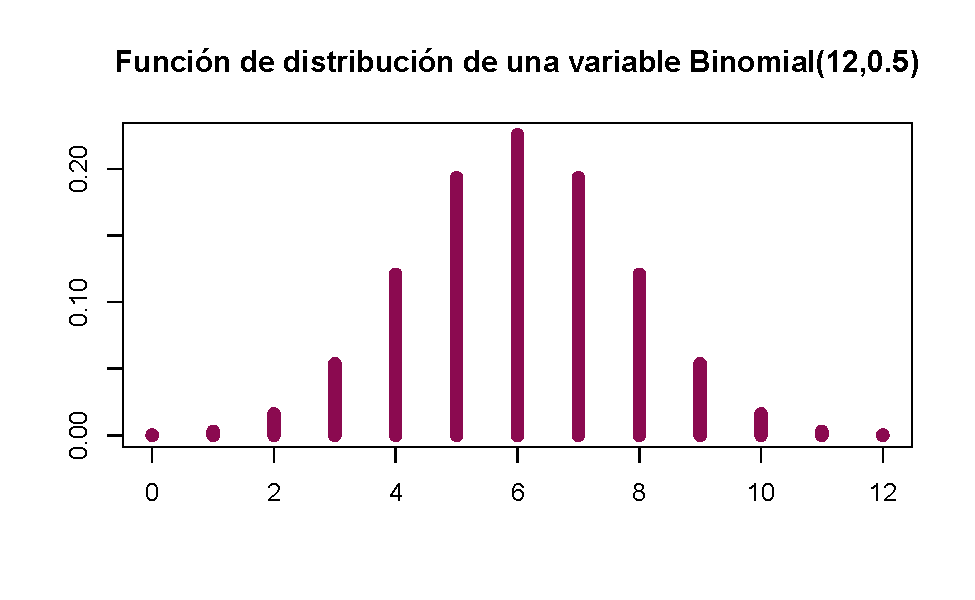
\includegraphics{_main_files/figure-latex/unnamed-chunk-22-1} \end{center}

Calculamos \(t\) y el \(p-value\):

\begin{Shaded}
\begin{Highlighting}[]
\NormalTok{t}\OtherTok{=}\FunctionTok{qbinom}\NormalTok{(.}\DecValTok{05}\NormalTok{,n,p)       }\CommentTok{\#Cuantil a comparar con el estadístico}
\NormalTok{t}
\end{Highlighting}
\end{Shaded}

\begin{verbatim}
[1] 3
\end{verbatim}

\begin{Shaded}
\begin{Highlighting}[]
\NormalTok{pvalue}\OtherTok{=}\FunctionTok{pbinom}\NormalTok{(T\_1,n,p)  }\CommentTok{\#p{-}value}
\NormalTok{pvalue}
\end{Highlighting}
\end{Shaded}

\begin{verbatim}
[1] 0.387207
\end{verbatim}

Tenemos que como \(T=5\nleq 3 =t\), entonces NO se rechaza \(H_0\) y por lo tanto se concluye que NO hay información suficiente para decir que la tasa promedio de descarga mensual este disminuyendo.

Finalmente utilizaremos la función en R:

\begin{Shaded}
\begin{Highlighting}[]
\FunctionTok{binom.test}\NormalTok{(}\DecValTok{5}\NormalTok{,n,}\AttributeTok{p=}\FloatTok{0.5}\NormalTok{,}\AttributeTok{alternative =} \StringTok{"less"}\NormalTok{)}
\end{Highlighting}
\end{Shaded}

\begin{verbatim}
    Exact binomial test

data:  5 and n
number of successes = 5, number of trials = 12, p-value = 0.3872
alternative hypothesis: true probability of success is less than 0.5
95 percent confidence interval:
 0.0000000 0.6847622
sample estimates:
probability of success 
             0.4166667 
\end{verbatim}

\begin{Shaded}
\begin{Highlighting}[]
\NormalTok{x}\OtherTok{=}\FunctionTok{c}\NormalTok{(}\FloatTok{14.6}\NormalTok{,}\FloatTok{14.2}\NormalTok{,}\FloatTok{12.2}\NormalTok{,}\FloatTok{10.5}\NormalTok{,}\DecValTok{104}\NormalTok{,}\DecValTok{123}\NormalTok{,}\DecValTok{220}\NormalTok{,}\DecValTok{190}\NormalTok{,}\DecValTok{110}\NormalTok{,}\DecValTok{138}\NormalTok{,}\DecValTok{86}\NormalTok{,}\FloatTok{98.1}\NormalTok{,}\FloatTok{92.8}\NormalTok{,}\FloatTok{88.1}\NormalTok{,}\FloatTok{74.4}\NormalTok{,}\DecValTok{80}\NormalTok{,}\FloatTok{75.4}\NormalTok{,}\FloatTok{75.6}\NormalTok{,}\FloatTok{51.7}\NormalTok{,}\FloatTok{48.8}\NormalTok{,}\FloatTok{29.3}\NormalTok{,}\FloatTok{27.1}\NormalTok{,}\DecValTok{16}\NormalTok{,}\FloatTok{15.7}\NormalTok{)}


\FunctionTok{library}\NormalTok{(randtests)}
\FunctionTok{cox.stuart.test}\NormalTok{(x)}
\end{Highlighting}
\end{Shaded}

\begin{verbatim}
    Cox Stuart test

data:  x
statistic = 4, n = 12, p-value = 0.3877
alternative hypothesis: non randomness
\end{verbatim}

\hypertarget{ejercicios}{%
\chapter{Ejercicios}\label{ejercicios}}

\textbf{1.} Un fabricante de teléfonos móviles afirma que sólo el 5\% de todas las unidades que vende sufre una falla durante el primer mes de operación normal. Una organización de consumidores ha pedido a 45 consumidores que han adquirido estos teléfonos móviles, que reporten cualquier mal funcionamiento durante el primer mes. Al final de éste sólo siete consumidores reportaron mal funcionamiento. Si la organización de consumidores cree que la proporción de teléfonos que sufrirán alguna falla es mayor al valor afirmado por el fabricante. ¿Con una \(\alpha\) del 10\% podría la organización sustentar su creencia?

\textbf{2.} Un candidato a través de encuestas propias afirma que el 65\% o más de los votantes están a su favor. Sin embargo, a través de una encuesta a 20 personas, 10 están a su favor. Probar que a un nivel de significancia del 5\%, la hipótesis de que el candidato a sobrestimado los votos a su favor.

\textbf{3.} En una muestra de 150 partidos de básquetbol universitario, el equipo de casa ganó 98 partidos. Realice una prueba para determinar si los datos sustentan la hipótesis de que en el básquetbol universitario el equipo de casa tiene ventaja. ¿A qué conclusión llega con \(\alpha= 0.05\)?

\textbf{4.} Una muestra aleatoria de niños de tercer año de secundaria mostró las siguientes observaciones de peso (kg)

\[
\begin{array}{|c| |c| |c| |c| |c|} 
\hline
64& 60& 44& 54& 61\\
46& 66& 56& 42& 62\\
39& 54& 68& 64& 65\\
75& 38& 53& 58&46\\
\hline
\end{array}
\]

Probar:

\begin{enumerate}
\def\labelenumi{\alph{enumi})}
\item
  La mediana de los pesos es 46kg.
\item
  El cuartíl superior es al menos 60kg.
\item
  El tercer decil no es mayor a 45kg.
\end{enumerate}

\textbf{5.} La siguiente es una muestra de 15 departamentos nuevos de 2 recamaras con estacionamiento en la colonias Roma, Condesa y Escandón. Los datos están en millones de pesos.

\[
\begin{array}{|c| |c| |c|} 
\hline
6.4&    5&  4.2\\
4.6&    4.4&    5.6\\
3.5&    3.8&    4.5\\
7.5&    5.6&    4.2\\
8.1&    5.8&    6.3\\
\hline
\end{array}
\]

Probar:

\begin{enumerate}
\def\labelenumi{\alph{enumi})}
\item
  Cuando menos 50\% de las observaciones están por debajo de los 4.3 millones.
\item
  No mas del 20\% de las observaciones tienen un costo mayor a 7 millones.
\end{enumerate}

\textbf{6.} En una encuesta anual para determinar si los salarios en el sector federal son proporcionales con los pagos en el sector privado, los trabajadores publicos y privados fueron emparejados tan cerca como fue posible (con respecto al tipo de trabajo, formación académica, años de experiencia, etc.) los salarios se ordenaron en parejas.

\[
\begin{array}{||c| |c| |c||} 
\hline 
\textbf{Pareja i}  & \textbf{Privado} & \textbf{Gobierno} \\ 
\hline
\hline
1 &12,500& 11,750 \\
\hline
\hline
2& 22,300 &20,900 \\
\hline
\hline
3 &14,500 &14,800 \\
\hline
\hline
4 &32,300 &29,900 \\
\hline
\hline
5 &20,800 &20,500 \\
\hline
\hline
6 &19,200 &18,400 \\
\hline
\hline
7 &15,800 &14,500 \\
\hline
\hline
8 &17,500 &17,900 \\
\hline
\hline
9 &23,300 &21,400 \\
\hline
\hline
10 &42,100 &43,200 \\
\hline
\hline
11 &16,800 &15,200 \\
\hline
\hline
12& 14,500 &14,200 \\
\hline
\hline
\end{array}
\]

Probar la hipótesis nula de que los salarios son iguales contra la hipótesis alternativa de que el salario de los trabajadores federales es generalmente menor a la contraparte en el sector privado. Uitiliza \(\alpha=0.1\).

\textbf{7.} Una oficina tiene dos computadoras : A y B. En un estudio del uso del ordenador, la compañía ha recabado registro de las tasas de uso por 5 semanas. La meta es decidir cual computadora se pone bajo un contrato de servicio porque tiene una tasa alta de uso. Con los datos de las tasas de uso de la siguiente tabla se puede hacer una recomendación preliminar respecto a que computadora contratar?

\[
\begin{array}{||c| |c| |c||} 
\hline 
\textbf{Semanas} & \textbf{Computadora A} & \textbf{Computadora B} \\ 
\hline
\hline
1 &15.7& 32.4 \\
\hline
\hline
2& 10.8 &41.2 \\
\hline
\hline
3 &45   & 35.1 \\
\hline
\hline
4 &12.3& 25 \\
\hline
\hline
5 & 8.2&8.2 \\
\hline
\hline
\end{array}
\]

\textbf{8.} Se tienen dos trituradores de alimentos y se tiene la sospecha de que el aparato B es mas eficiente que el aparato A. Para probar dicha sospecha, se probaron en ambos trituradores diferentes alimentos y se registró el tiempo en minutos que le tomaba a cada aparato convertir el alimento en puré. Los resultados fueron los siguientes.

\[
\begin{array}{||c| |c| |c| |c|} 
\hline 
\mbox{Alimento} & \mbox{A} & \mbox{B}\\
 \hline
1&0.5&0.6\\
 \hline
2&1&0.9\\
 \hline
3&1.2&1.2\\
 \hline
4&0.8&0.9\\
 \hline
5&0.4&0.5\\
 \hline
6&1.5&1.8\\
 \hline
7&0.3&0.4\\
 \hline
8&1.2&1.4\\
 \hline
9&0.7&0.9\\
\hline
\hline
\end{array}
\]

Con los datos observados se puede corroborar la sospecha en cuanto a la eficiencia de los trituradores? Use \(\alpha=5\%\)

\textbf{9.} Se toma una muestra aleatoria de 135 ciudadanos de E.U. y se les preguntó su opinión con respecto a cierta política. El estudio registró a 43 ciudadanos que estaban en contra de esa política. Después de varias semanas, durante las cuales los ciudadanos recibieron cartas informativas, se les volvió a preguntar su opinión; 37 estuvieron en contra, y 30 de las 37 originalmente no estaban en contra de la política. ¿Es significativo el cambio en el número de personas en contra de la política?

\textbf{10.} Un investigador intenta determinar si un fármaco tiene un efecto sobre una enfermedad particular. Se cuenta con la información de los individuos en el estudio con el diagnóstico (enfermedad: presente o ausente ) antes del tratamiento, y el diagnóstico después del tratamiento

\[
\begin{array}{c| c c|c} 
&\mbox{Después de tratamiento}&&\\
\hline
\mbox{Antes de tratamiento}& \textbf{Presente} & \textbf{Ausente} & \mbox{Total} \\  
\hline
\textbf{Presente} & 101& 121&222\\
\hline
\textbf{Ausente} & 59& 33&92\\
\hline
\mbox{Total}&160&154&314\\
\end{array}
\]

\textbf{11.} Un programa ecológico sobre la contaminación de un río tomó 5 muestras de agua de diferentes lugares de un río antes y después de dos años, obteniéndose los siguientes resultados. Los números representan la media de la contaminación, donde medidas grandes indican alta contaminación.

\[
\begin{array}{||c| |c| |c||} 
\hline 
\textbf{Numero de Muestras} & \textbf{Medidas iniciales} & \textbf{Medidas después de 2 años}  \\  
\hline
\hline
1 &88.4& 87.1 \\
\hline
\hline
2& 81.3 &79.4 \\
\hline
\hline
3 &68.4 & 69.1 \\
\hline
\hline
4 &100.5& 91.1 \\
\hline
\hline
5 & 93.2&95.3 \\
\hline
\hline
\end{array}
\]

Se está interesado en saber si el programa de rehabilitación ecológica ha tenido efecto en la reducción de la contaminación. Use \(\alpha =1\%\).

\textbf{12.} Se presentan a continuación los tipos de cambio MXN-USD de los últimos 30 días.

24.48 ,
24.07 ,
23.66 ,
23.70 ,
23.93 ,
24.34 ,
24.22 ,
23.87 ,
23.96 ,
24.05 ,
23.78 ,
23.74 ,
23.21 ,
22.88 ,
22.74 ,
22.73 ,
22.58 ,
22.21 ,
22.33 ,
22.21 ,
22.17 ,
22.21 ,
22.04 ,
21.79 ,
21.76 ,
21.91 ,
21.58 ,
21.60 ,
21.50 ,
21.91

Se desea corroborar la aseveración del presidente respecto a que el peso mexicano esta recuperando fuerza. Use \(\alpha=10\%\).

\hypertarget{part-prueba-de-rango}{%
\part{Prueba de Rango}\label{part-prueba-de-rango}}

\hypertarget{introducciuxf3n-2}{%
\chapter*{Introducción}\label{introducciuxf3n-2}}


Ya nos empapamos de la pruebas binomiales ahora en esta seccion se presentan tres de las pruebas de rangos más utilizadas en modelos no paramétricos, la prueba de Mann y Witney, la prueba de Kruskal-Wallis y la prueba de Igualdad de Varianzas.

Estas pruebas son otros métodos no paramétrico que se usan para determinar si hay diferencia entre poblaciones. El procedimiento se basa en ordenar las observaciones pertenecientes a muestras aleatorias de cada población, asignarles rangos según sus valores y posteriormente construir la prueba sobre dichos rangos.

\hypertarget{prueba-u-mann-y-witney}{%
\chapter{Prueba U-Mann y Witney}\label{prueba-u-mann-y-witney}}

Esta prueba está diseñada para determinar si dos muestras han sido extraídas de la misma población.La prueba también es conocida como Mann-Whitney-Wilcoxon o suma de rangos de Wilcoxon.

A diferencia de las pruebas binomiales bivariadas vistas en la sección anterior, esta no se basa en una muestra por pares. En lugar usa dos muestras independientes, una de cada población a probar.

\hypertarget{datos-5}{%
\section{Datos}\label{datos-5}}

Se considera que los datos provienen de dos muestras aleatorias:

\[x_{1},x_{2},x_{3},\cdots,x_{n} \ \mbox{una muestra aleatoria de tamaño} \ n \ \mbox{de la población.}\]

\[y_{1},y_{2},y_{3},\cdots,y_{m} \ \mbox{una muestra aleatoria de tamaño} \  m \  \mbox{de la poblacion.}\]

De forma conveniente, tomamos \(N=n+m\).

Sea:

\[F(t) \ \mbox{la función de distribución de probabilidad de X.}\]

\[G(t) \ \mbox{la función de distribución de probabilidad de Y.}\]

\hypertarget{supuestos-5}{%
\section{Supuestos}\label{supuestos-5}}

\begin{enumerate}
\def\labelenumi{\arabic{enumi})}
\item
  Independencia dentro de cada muestra.
\item
  Independencia entre muestras.
\item
  La escala de medida es al menos ordinal.
\end{enumerate}

\textbf{Pasos a seguir}

\begin{enumerate}
\def\labelenumi{\arabic{enumi}.}
\item
  Formar una nueva muestra combinada de los \(n+m\) datos
\item
  Ordenar de menor a mayor
\item
  Asignamos el rango correspondiente
\item
  Si hay empates entonces asignamos el promedio de los rangos
\end{enumerate}

\hypertarget{estaduxedstico-de-prueba-5}{%
\section{Estadístico de Prueba}\label{estaduxedstico-de-prueba-5}}

\begin{itemize}
\tightlist
\item
  \textbf{Si no hay empates}
\end{itemize}

\[T=\sum_{i=1}^{n}R(X_{i})\]

\begin{itemize}
\tightlist
\item
  \textbf{Si hay empates}
\end{itemize}

\[T_1= \frac{T-n\frac{N+1}{2}}{\sqrt{\frac{nm}{N(N-1)}\sum_{i=1}^{N}R_i^2-\frac{nm(N+1)^2}{4(N-1)}}}\]

\[T_{1}\sim N(0,1)\]

Dependiendo del planteamiento de nuestro problema a resolver se formulan las hipótesis:

\hypertarget{hipuxf3tesis-5}{%
\section{Hipótesis}\label{hipuxf3tesis-5}}

\hypertarget{caso-a-prueba-de-dos-colas-5}{%
\subsection*{Caso A (Prueba de dos colas)}\label{caso-a-prueba-de-dos-colas-5}}


\[\textbf{H}_0: F(x) = G(x) \ \  \forall\ x, \ \ \  \mbox{alternativo} \ \ \  \textbf{H}_0:\mathbf{E}[X] = \mathbf{E}[Y]\]

\[vs\]

\[\textbf{H}_a: F(x) \neq G(x) \ \ \mbox{para alguna} \ x,  \ \ \mbox{alternativo} \ \ \  \textbf{H}_a:
\mathbf{E}[X] \neq \mathbf{E}[Y]\]

\hypertarget{regla-de-decisiuxf3n-13}{%
\subsubsection*{Regla de decisión}\label{regla-de-decisiuxf3n-13}}


Rechazamos \(H_0\) a un nivel de significancia \(\alpha\) si

\[T < t_{\frac{\alpha}{2}} \ \ \   o \ \ \ T > t_{1-\frac{\alpha}{2}}\]

Donde \(t_\frac{\alpha}{2}\) el cuantil inferior se busca en las tablas correspondientes a nuestra prueba.

Y \(t_{1-\frac{\alpha}{2}}\) el cuantil superior se calcula de la siguiente manera:

\[\omega_p= n(n+m+1)-\omega_{1-p}\]
donde \(\omega_{1-p}\) es el cuantil inferior obtenido de la tabla correspondiente a nuestra prueba.

Los cuantiles aproximados en el caso de no tener empates, y \(n\) o \(m\) mayores a 20, se encuentra la aproximacion normal.

\[\omega_p= \frac{n(N+1)}{2} + z_p\sqrt{\frac{n m(N+1)}{12}}\]

donde el cuantil \(z_p\) se obtiene de la tabla de la distribución normal.

y calculamos el \(p-value\)de la siguiente manera:

\[p-value = 2*\mathbf{P}\left(Z\leq\frac{T+\frac{1}{2}-n\frac{N+1}{2}}{\sqrt{\frac{nm(N+1)}{12}}}\right)\]
Donde \(Z\) es la variable aleatoria normal estándar.

\begin{itemize}
\tightlist
\item
  Si ocupamos \(T_{1}\), rechazamos \(H_0\) si:
\end{itemize}

\[T_{1} < z_{\frac{\alpha}{2}} \ \ \  o \ \ \  T_{1} > z_{1-\frac{\alpha}{2}}\]

Donde \(z_\frac{\alpha}{2}\) y \(z_{1-\frac{\alpha}{2}}\) son cuantiles que se buscan en la tabla de una normal estándar.

y calculamos el \(p-value\)de la siguiente manera:

\[p-value=2*min\{\mathbf{P}[Z\leq T_{1}],\mathbf{P}[Z\geq T_{1}]\}\]
Donde \(Z\) es la variable aleatoria normal estándar.

\hypertarget{caso-b-prueba-de-cola-inferior-4}{%
\subsection*{Caso B (Prueba de cola inferior)}\label{caso-b-prueba-de-cola-inferior-4}}


\[\textbf{H}_0: F(x) = G(x) \ \ vs \ \ \textbf{H}_a: F(x) > G(x),  \ \ \mbox{alternativo} \ \ \textbf{H}_a:\mathbf{E}[X]  < \mathbf{E}[Y]\]

\hypertarget{regla-de-decisiuxf3n-14}{%
\subsubsection*{Regla de decisión}\label{regla-de-decisiuxf3n-14}}


Rechazamos \(H_0\) a un nivel de significancia \(\alpha\) si

\[T < t_{\alpha}\]

Donde \(t_{\alpha}\) el cuantil inferior se busca en las tablas correspondientes a nuestra prueba.

Los cuantiles aproximados en el caso de no tener empates, y \(n\) o \(m\) mayores a 20, se encuentra la aproximacion normal.

\[\omega_p= \frac{n(N+1)}{2} + z_p\sqrt{\frac{n m(N+1)}{12}}\]
donde el cuantil \(z_p\) se obtiene de la tabla de la distribución normal.

y calculamos el \(p-value\) de la siguiente manera:

\[p-value = \mathbf{P}\left(Z\leq\frac{T+\frac{1}{2}-n\frac{N+1}{2}}{\sqrt{\frac{nm(N+1)}{12}}}\right)\]
* Si ocupamos \(T_{1}\), rechazamos \(H_0\) si:

\[T_{1} < z_{\alpha}\]

Donde \(z_{\alpha}\) es el cuantil que se buscan en la tabla de una normal estándar.

y calculamos el \(p-value\) de la siguiente manera:

\[p-value=\mathbf{P}[Z\leq T_{1}]\]
Donde \(Z\) es la variable aleatoria normal estándar.

\hypertarget{caso-c-prueba-de-cola-superior-3}{%
\subsection*{Caso C (Prueba de cola superior)}\label{caso-c-prueba-de-cola-superior-3}}


\[\textbf{H}_0: F(x) = G(x) \ \ vs \ \ \textbf{H}_a: F(x) < G(x), \  \ \mbox{alternativo} \ \ \textbf{H}_a:\mathbf{E}[X]  > \mathbf{E}[Y]\]

\hypertarget{regla-de-decisiuxf3n-15}{%
\subsubsection*{Regla de decisión}\label{regla-de-decisiuxf3n-15}}


Rechazamos \(H_0\) a un nivel de significancia \(\alpha\) si

\[T > t_{1-{\alpha}}\]
Y \(t_{1-\alpha}\) el cuantil superior se calcula de la siguiente manera:

\[\omega_p= n(n+m+1)-\omega_{1-p}\]
donde \(\omega_{1-p}\) es el cuantil inferior obtenido de la tabla correspondiente a nuestra prueba.

Los cuantiles aproximados en el caso de no tener empates, y \(n\) o \(m\) mayores a 20, se encuentra la aproximacion normal.

\[ \omega_p= \frac{n(N+1)}{2} + z_p\sqrt{\frac{n m(N+1)}{12}}\]
donde el cuantil \(z_p\) se obtiene de la tabla de la distribución normal.

y calculamos el \(p-value\) de la siguiente manera:

\[p-value = \mathbf{P}\left(Z\geq\frac{T+\frac{1}{2}-n\frac{N+1}{2}}{\sqrt{\frac{nm(N+1)}{12}}}\right)\]

\begin{itemize}
\tightlist
\item
  Si ocupamos \(T_{1}\), rechazamos \(H_0\) si:
\end{itemize}

\[T_{1} > z_{1-\alpha}\]

Donde \(z_{1-\alpha}\) es el cuantil que se buscan en la tabla de una normal estándar.

y calculamos el \(p-value\) de la siguiente manera:

\[p-value=\mathbf{P}[Z\geq T_{1}] \ \ o \ \  \ 1-\mathbf{P}[Z\leq T_{1}]\]
Donde \(Z\) es la variable aleatoria normal estándar.

Tal vez es demasiada información que procesar asi que veremos un ejemplo paso por paso:

\hypertarget{ejemplo-5}{%
\section{Ejemplo}\label{ejemplo-5}}

Una agencia publicitaria está investigando a qué tipo de avisos les prestan más atención los adolescentes. Se observan a 11 adolescentes, a 6 de ellos se les muestran anuncios de comida y a los 5 restantes se les muestran anuncios de bebidas; todos los anuncios tienen una duración similar y a continuación se muestra el registro del tiempo de atención (en segundos) de los 11 adolescentes.
Utilizaremos \(\alpha\)= 5\%.

\[
\begin{array}{||c| c c c c c c||} 
\hline
\textbf{Comida} & 25 & 41 & 42 & 45 & 47 & 50 \\
\hline\hline
\textbf{Bebidas}& 23 & 28 & 30 & 35 & 38 &  \\ 
\hline
\end{array}
\]

Podemos ver que m=6 (en este caso comidas) y n= 5 (en este caso bebidas)

\textbf{Paso 1} Escribimos la prueba a utilizar

La prueba a utilizar \textbf{Prueba U-Mann-Whitney - Caso A - dos colas}

\textbf{Paso 2} Formulamos nuestras hipótesis en contexto al problema planteado

\[\textbf{H}_0: \ \mbox{La distribución del tiempo de atención que prestan los adolescentes a los 
anuncios}\]
\[\mbox{sobre comida es igual a la distribución de los anuncios de bebidas.}\]

\[vs\]

\[\textbf{H}_a: \ \mbox{La distribución del tiempo de atención que prestan los adolescentes a los anuncios}\]
\[\mbox{sobre comida es distinta a las distribución de los anuncios de bebidas.}\]

\textbf{Ordenamos de menor a mayor}

\[
\begin{array}{ |c| c c c c c c c c c c c| }
\hline
 \textbf{Tipo de aviso} & B & C & B & B & B & B & C & C & C & C & C \\ 
 \hline
 \textbf{Dato ordenado} & 23 & 25 & 28 & 30 & 35 & 38 & 41 & 42 & 45 & 47 & 50 \\ 
 \hline
 \textbf{Rango}         & 1 & 2 & 3 & 4 & 5 & 6 & 7 & 8 & 9 & 10 & 11 \\ 
 \hline
\end{array}
\]

\textbf{Paso 3} Estadístico de prueba

Como no tenemos empates utilizaremos el estadistico T:

\[T=\sum_{i=1}^{n}R(X_{i})\]

\textbf{Paso 4} Procedimiento completo

\[T=\sum_{i=1}^{5}R(X_{i})= 1+3+4+5+6= 19\]

\textbf{Paso 5} Regla de decisión

Rechazamos \(H_0\) a un nivel de significancia \(\alpha\)=.05 si

\[T < t_\frac{\alpha}{2} \ \ \  \ \  o  \ \ \ \ \  T > t_{1-\frac{\alpha}{2}}\]

El valor del cuantil inferior localizado en las tablas es 19, y por otro lado vamos a calcular el cuantil superior:

\[\omega_p= n(n+m+1)-\omega_{1-p}\]
\[\omega_p= 5(5+6+1)-19\]
\[\omega_p= 41\]

\[19 \nless   19  \ \ \  o \ \ \  19 \ngtr 41\]

\(\therefore\) No rechazo \(H_0\)

\textbf{Calculamos p-value}

\[p-value = 2*\mathbf{P}\left(Z\leq\frac{T+\frac{1}{2}-n\frac{N+1}{2}}{\sqrt{\frac{nm(N+1)}{12}}}\right)\]
\[p-value = 2*\mathbf{P}\left(Z\leq\frac{19+\frac{1}{2}-5\frac{12}{2}}{\sqrt{\frac{5*6(12)}{12}}}\right)=0.028\]
\[p-value = 2*0.028\]
\[p-value = 0.056\]

Ya que \(p-value > \alpha\)

\(\therefore\) No rechazo \(H_0\)

\textbf{Paso 6} Conclusión

\(\therefore\) No hay diferencia significativa en el tiempo de atención de los adolescentes en los anuncios de comida y bebidas.

\hypertarget{ejemplo-en-r-studio-5}{%
\section{Ejemplo en R-Studio}\label{ejemplo-en-r-studio-5}}

Ahora haremos la réplica en R.

El primer paso es ordenar los rangos:

\begin{Shaded}
\begin{Highlighting}[]
\NormalTok{R\_i}\OtherTok{=}\FunctionTok{c}\NormalTok{(}\DecValTok{1}\NormalTok{,}\DecValTok{2}\NormalTok{,}\DecValTok{3}\NormalTok{,}\DecValTok{4}\NormalTok{,}\DecValTok{5}\NormalTok{,}\DecValTok{6}\NormalTok{,}\DecValTok{7}\NormalTok{,}\FloatTok{8.5}\NormalTok{,}\FloatTok{8.5}\NormalTok{,}\DecValTok{10}\NormalTok{,}\DecValTok{11}\NormalTok{)}
\end{Highlighting}
\end{Shaded}

El segundo paso es calcular \(T\) que corresponde a la suma de los rangos asignados a los anuncios de ``Bebida''.

\begin{Shaded}
\begin{Highlighting}[]
\NormalTok{T}\OtherTok{=}\DecValTok{1}\SpecialCharTok{+}\DecValTok{3}\SpecialCharTok{+}\DecValTok{4}\SpecialCharTok{+}\DecValTok{5}\SpecialCharTok{+}\DecValTok{6}  \CommentTok{\#rangos asignados a los anuncios de bebida}
\NormalTok{T}
\end{Highlighting}
\end{Shaded}

\begin{verbatim}
[1] 19
\end{verbatim}

\begin{Shaded}
\begin{Highlighting}[]
\NormalTok{n}\OtherTok{=}\DecValTok{5}
\NormalTok{m}\OtherTok{=}\DecValTok{6}
\NormalTok{N}\OtherTok{=}\NormalTok{n}\SpecialCharTok{+}\NormalTok{m}
\end{Highlighting}
\end{Shaded}

Según el planteamiento de las hipótesis, este es un Caso A (de 2 colas), por lo que siguiendo la regla de decisión, se rechazará \(H_0\) si \(T \leq t_1\) o \(T> t_2\), donde \(t_1\) es el cuantil que acumula \(2.5\%\) de probabilidad en una distribución normal estándar, y \(t_2\) es el cuantil que acumula \(97.5\%\) en la misma distribución.

\begin{Shaded}
\begin{Highlighting}[]
\NormalTok{t1}\OtherTok{=}\DecValTok{19}
\NormalTok{t1}
\end{Highlighting}
\end{Shaded}

\begin{verbatim}
[1] 19
\end{verbatim}

\begin{Shaded}
\begin{Highlighting}[]
\NormalTok{t2}\OtherTok{=}\DecValTok{41}
\NormalTok{t2}
\end{Highlighting}
\end{Shaded}

\begin{verbatim}
[1] 41
\end{verbatim}

\begin{Shaded}
\begin{Highlighting}[]
\NormalTok{pvalue}\OtherTok{=}\DecValTok{2}\SpecialCharTok{*}\FloatTok{0.028}
\NormalTok{pvalue}
\end{Highlighting}
\end{Shaded}

\begin{verbatim}
[1] 0.056
\end{verbatim}

Observamos que \(T \leq t_1\) por lo tanto rechazaremos \(H_0\) y concluimos que la distribución del tiempo de atención que prestan los adolescentes a los anuncios sobre comida es distinta a la distribución del tiempo de atención prestada a los anuncios de bebidas.

En R la prueba \textbf{``wilcox.test''} también realiza esta prueba con un cálculo ligeramente distinto de la estadística de prueba. En el caso de la prueba de Wilcoxon lo que contaremos es el número de ocasiones que la \(x_i>y_j\) para todas las combinaciones de \(i=1,...n\) y \(j=1,...,m\).

Si las distribuciones son iguales entonces se esperaría que el número de veces que \(x_i>y_j\) sea cercano a la mitad de las combinaciones.

\begin{Shaded}
\begin{Highlighting}[]
\NormalTok{B}\OtherTok{=}\FunctionTok{c}\NormalTok{(}\DecValTok{23}\NormalTok{, }\DecValTok{28}\NormalTok{, }\DecValTok{30}\NormalTok{, }\DecValTok{35}\NormalTok{, }\DecValTok{38}\NormalTok{)     }\CommentTok{\#Datos de bebidas}
\NormalTok{C}\OtherTok{=}\FunctionTok{c}\NormalTok{(}\DecValTok{25}\NormalTok{, }\DecValTok{41}\NormalTok{, }\DecValTok{42}\NormalTok{, }\DecValTok{45}\NormalTok{, }\DecValTok{47}\NormalTok{, }\DecValTok{50}\NormalTok{) }\CommentTok{\#DAtos de comidas}
\NormalTok{m1}\OtherTok{\textless{}{-}}\FunctionTok{wilcox.test}\NormalTok{(B,C, }\AttributeTok{na.rm=}\ConstantTok{TRUE}\NormalTok{, }\AttributeTok{paired=}\ConstantTok{FALSE}\NormalTok{, }\AttributeTok{exact=}\ConstantTok{FALSE}\NormalTok{)}
\FunctionTok{print}\NormalTok{(m1)}
\end{Highlighting}
\end{Shaded}

\begin{verbatim}
    Wilcoxon rank sum test with continuity correction

data:  B and C
W = 4, p-value = 0.05523
alternative hypothesis: true location shift is not equal to 0
\end{verbatim}

Con esta prueba se rechaza la hipótesis nula de que ambas distribuciones son iguales. Y se concluye de la misma forma que la prueba de rangos anterior. La distribución del tiempo de atención que prestan los adolescentes a los anuncios sobre comida es distinta a la distribución del tiempo de atención prestada a los anuncios de bebidas.

\hypertarget{intervalo-de-confianza-para-la-diferencia-entre-dos-medias}{%
\chapter{Intervalo de confianza para la diferencia entre dos medias}\label{intervalo-de-confianza-para-la-diferencia-entre-dos-medias}}

\hypertarget{datos-6}{%
\section{Datos}\label{datos-6}}

Los datos consisten en dos muestras aleatorias \(X_{1}, \ldots, X_{n}\) y \(Y_{1}, \ldots, Y_{m}\) de tamaño \(n\) y \(m\), respectivamente. Sea \(X\) y \(Y\) las variables aleatorias con la misma distribución que las \(X_{i}\) y las \(Y_{j}\), respectivamente.

\hypertarget{supuestos-6}{%
\section{Supuestos}\label{supuestos-6}}

\begin{enumerate}
\def\labelenumi{\arabic{enumi})}
\item
  Ambas muestras son muestras aleatorias de sus respectivas poblaciones.
\item
  Además de la independencia dentro de cada muestra, existe mutua independencia entre las dos muestras.
\item
  Las dos funciones de distribución de la población son idénticas, excepto por una posible diferencia en los parámetros de ubicación. Es decir, hay una constante \(d\) (por ejemplo) tal que \(X\) tiene la misma función de distribución que \(Y + d\).
\end{enumerate}

\hypertarget{muxe9todo}{%
\section{Método}\label{muxe9todo}}

Determine el cuantil \(\alpha/2\) (\(\omega_{\alpha/2}\)) para \(n\) y \(m\) de las tablas correspondientes a \textbf{Prueba Mann-Whitney}, o si \(n\) y \(m\) son mayores a 20 se ocupa la aproximación del cuantil, donde \(1-\alpha\) es el coeficiente de confianza.Note que esto se puede utilizar incluso si hay muchos empates.

Luego calcule \(k\), dado por:

\[k= \omega_{\alpha/2}-n(n+1)/2\]

Para todos los pares posibles (\(X_{i},Y_{j}\)), encuentre las \(k\) diferencias más grandes \(X_{i}-Y_{j}\) y encontrar las \(k\) diferencias más pequeñas.

Para encontrar las diferencias más grandes y más pequeñas, es conveniente ordenar primero cada muestra, de menor a mayor, y luego formar una matriz de diferencias \(X_{i}-Y_{j}\) usando las \(X_s\) como filas y las \(Y_s\) como columnas.

La k-ésima diferencia más grande es el límite superior \(U\) y la \(k-ésima\) diferencia más pequeña es el límite inferior \(L\).

Entonces el intervalo de confianza es obtenido por:

\[\mathbf{P}[L\leq \mathbf{E}(X)-\mathbf{E}(Y)\leq U]\geq 1-\alpha\]

Ahora haremos un ejemplo para ilustrar la teoría:

\hypertarget{ejemplo-6}{%
\section{Ejemplo}\label{ejemplo-6}}

Se desea mezclar una masa de pastel hasta que se alcance una consistencia específica. Se mezclan cinco lotes de la mezcla usando la batidora A, y los otros cinco lotes se mezclan usando la batidora B. Los tiempos requeridos para mezclar se dan de la siguinte manera (en minutos):

\[
\begin{array}{c c}
\textbf{Batidora A} & \textbf{Batidora A} \\
7.3 & 7.4 \\
6.9 & 6.8  \\
7.2 & 6.9 \\
7.8 & 6.7 \\
7.2 & 7.1 \\
\end{array}
\]
Se busca un intervalo de confianza del 95\% para la diferencia de medias en los tiempos de mezcla, más específicamente para \(\mathbf{E}(X)-\mathbf{E}(Y)\), donde \(X\) se refiere a la \(batidora\ A\) y \(Y\) se refiere a la \(batidora\ B\).

\textbf{Paso 1}

Encontrar cuantil \(\alpha/2\) (\(\omega_{\alpha/2}\)), para nuestro ejemplo \(n\)=5, \(m\)=5, \(\alpha=0.05\), y buscando en la \textbf{Tabla Mann-Whitney} tenemos \(\omega_{\alpha/2}=\omega_{0.025}=18\)

\textbf{Paso 2}

Calculamos \(k\), dado por:

\[k= \omega_{\alpha/2}-n(n+1)/2\]

\[k=18-(5)(6)/2=3\]

\textbf{Paso 3}

Ordenamos las muestras de menor a mayor, las \(X_s\) las usaremos como filas y las \(Y_s\) las usaremos como columnas para formar la matriz de diferencias \(X_{i}-Y_{j}\):

\[
\begin{array}{|l| r r r r r|}
\hline
X_{i} \ Y_{j} & 6.7 & 6.8 & 6.9 & 7.1 & 7.4 \\
\hline
6.9 & 0.2 & 0.1 & 0.0 & -0.2 & -0.5 \\
7.2 & 0.5 & 0.4 & 0.3 &  0.1 & -0.2 \\
7.2 & 0.5 & 0.4 & 0.3 &  0.1 & -0.2 \\
7.3 & 0.6 & 0.5 & 0.4 &  0.2 & -0.1 \\
7.8 & 1.1 & 1.0 & 0.9 &  0.7 &  0.4 \\
\hline
\end{array}
\]

\textbf{Paso 4}

Entonces las más grandes y las más pequeñas diferencias son encontradas:

\[
\begin{array}{c c c c}
\mbox{Diferencias Pequeñas} & & \mbox{ Diferencias Grandes} \\
6.9 - 7.4 = -0.5 & & 7.8 - 6.7 = 1.1\\
6.9 - 7.1 = -0.2 & & 7.8 - 6.8 = 1.0\\
7.2 - 7.4 = -0.2 = \textbf{L} & & 7.8 - 6.9 = 0.9 = \textbf{U}\\
\end{array}
\]

\textbf{Paso 5}

El intervalo de confianza del 95\% \((L,U)\) para la diferencia de medias, es decir, \(\mathbf{E}(X)-\mathbf{E}(Y)\) es \((-0.2,0.9)\).

\hypertarget{prueba-de-kruskal-wallis}{%
\chapter{Prueba de Kruskal-Wallis}\label{prueba-de-kruskal-wallis}}

Se obtienen \(k\) \(m.a.i.\) de \(k\) distintas poblaciones (\(k\geq 2\)) y queremos probar la hipótesis nula de que todas las poblaciones tienen la misma distribución contra la alternativa de que algunas de las poblaciones tienden a tener distribución distinta.
Un caso particular, si \(k=2\) se tiene la prueba de \textbf{Mann-Whitney}.

\hypertarget{datos-7}{%
\section{Datos}\label{datos-7}}

Se tienen \(k\ \ m.a.\) que pueden tener incluso distintos tamaños, la \(i-ésima\ \ m.a.\) de tamaño \(n_{i}\) es:
\[X_{i_1},\ X_{i_2},\ \cdots, \ X_{i_{ni}} \ \ (m.a. \mbox{de la} \ \ i-ésima \ \ \mbox{población.})\]

Así:

\[
\begin{array}{c c c c c} 
Muestra \ 1&Muestra\ 2&Muestra\ 3&...&Muestra\ k \\
x_{11}&x_{21}&x_{31}&...&x_{k1}\\
x_{12}&x_{22}&x_{32}&...&x_{k2}\\
\ldots&\ldots&\ldots&\ddots&\ldots\\
x_{1n_1}&x_{2n_2}&x_{3n_3}&...&x_{kn_k}\\
\end{array}
\]

sea \(N\) el número total de observaciones:

\[ N= \sum_{i=1}^{k} n_{i}\]

\hypertarget{supuestos-7}{%
\section{Supuestos}\label{supuestos-7}}

\begin{enumerate}
\def\labelenumi{\arabic{enumi})}
\item
  Todas las muestras son muestras aleatorias de sus respectivas poblaciones.
\item
  Además de la independencia dentro de las muestras, suponemos que hay independencia entre las muestras (es decir, las poblaciones son independientes).
\item
  Las \(k\) poblaciones son idénticas o algunas de las poblaciones tienden a tener valores más grandes que las otras poblaciones.
\item
  La escala de medida es al menos ordinal.
\end{enumerate}

\hypertarget{hipuxf3tesis-6}{%
\section{Hipótesis}\label{hipuxf3tesis-6}}

\[\textbf{H}_0: \ \mbox{Las funciones de distribución de las} \ \  k \ \ \mbox{poblaciones son idénticas.}\]

\[vs\]

\[\textbf{H}_a: \ \mbox{Al menos una de las poblaciones tiende a tener valores mayores que}\]

\[\mbox{al menos una de las poblaciones.}\]

\[\mbox{o equivalentemente}:\]

\[\textbf{H}_a: \mbox{Las} \ \ k \ \  \mbox{poblaciones no tienen medias idénticas.}\]

\textbf{Asignación de Rangos}

\begin{itemize}
\item
  Asignamos el rango \(1\) a la observación más pequeña de las \(N\) observaciones, el rango \(2\) a la \(2da\) más pequeña, y así sucesivamente hasta llegar a la observación mayor que recibirá el rango \(N\).
\item
  Sea \(R(X_{ij})\) el rango asignado a la observación \(X_{ij}\)
\item
  Sea \(R_{i}\) la suma de los rangos asignados a la \(i-ésima\) muestra (la \(i-ésima\) columna):
\end{itemize}

\[R_{i}=\sum_{j=1}^{n_{i}} R(X_{ij}),  i= 1, 2,\cdots,k\]

\textbf{NOTA}

Se calcula \(R_{i}\) para cada muestra, si hay observaciones repetidas, se le asigna el promedio de los rangos de las observaciones repetidas.

\[
\begin{array}{c c c c c} 
Rangos & Rangos & Rangos & \cdots  & Rangos \\
Muestra\ 1 & Muestra \ 2 & Muestra\ 3 & \cdots & Muestra\ k \\
\hline
R(X_{11}) &  R(X_{21}) & R(X_{31})  & \cdots & R(X_{k_{1}}) \\ 
R(X_{12}) &  R(X_{22}) & R(X_{31}) & \cdots & R(X_{k_{2}}) \\  
\vdots &  \vdots & \vdots  & \cdots &\vdots \\ 
R(X_{1n_{1}}) &R(X_{2n_{2}})   &R(X_{3n_{3}})   & \cdots &  R(X_{kn_{k}}) \\ 
\hline
R_{1} & R_{2} & R_{3} & \cdots&R_{k} \\
\end{array}
\]

\hypertarget{estaduxedstico-de-prueba-6}{%
\section{Estadístico de prueba}\label{estaduxedstico-de-prueba-6}}

\[T= \frac{1}{S^2}\left(\sum_{i=1}^{k}\frac{R^2_{i}}{n_{i}}-\frac{N(N+1)^2}{4}\right)\]
donde \(N\) y \(R_{i}\) son como los definimos anteriormente y donde:

\[ S^2 = \frac{1}{N-1}\left(\sum_{todos\ los\ rangos}R(X_{ij})^2-N\frac{(N+1)^2}{4}\right)\]
* \textbf{Si no hay empates} \(S^2\) se simplifica a \(N(N+1)/12\), y la estadística de prueba se reduce a:

\[ T= \frac{12}{N(N+1)}\sum_{i=1}^{k}\frac{R^2_{i}}{n_{i}}-3(N+1) \]

\hypertarget{regla-de-decisiuxf3n-16}{%
\section{Regla de decisión}\label{regla-de-decisiuxf3n-16}}

Rechazamos \(H_0\) al nivel de significancia \(\alpha\) si \(T>\omega_{1-\alpha}\), donde \(\omega_{1-\alpha}\) se obtiene de la tabla de cuantiles de la distribución de \(T\) (tablas Kruskal-Wallis). En caso de no encontrarse en la tabla, los tamaños de muestra correspondientes se utiliza la aproximación Ji-cuadrada con \(k-1\) grados de libertad para el estadístico de prueba.

Es decir, rechazamos \(H_0\) a un nivel \(\alpha\) si \(T > \chi^2_{(k-1)}(1-\alpha)\)

y calculamos el \(p-value\) de la siguiente manera el \(p-value\) es aproximadamente la probabilidad de una variable aleatoria chi-cuadrado con \(k-1\) grados de libertad que excede el valor observado de \(T\).

\textbf{Múltiples comparaciones}

Si y sólo si la hipótesis nula es rechazada, podriamos utilizar el siguiente procedimiento para determinar cuales pares de poblaciones tienden a ser diferentes.

Podemos decir que las poblaciones \(i\) y \(j\) parecen ser diferentes si se satisface la siguiente desigualdad:

\[\left|\frac{Ri}{ni}- \frac{Rj}{nj}\right|> t_{1-\alpha/2}\left(S^2\frac{N-1-T}{N-k}\right)^{1/2}\left(\frac{1}{n_i}+\frac{1}{n_j}\right)^{1/2}\]

Donde \(R_i\) y \(R_j\) son las sumas de los rangos de las dos muestras, \(t_{1-(\frac{\alpha}{2})}\) es el cuantil \(1-\frac{\alpha}{2}\) de la distribución \(t\) obtenida de las tablas de la distribución con \(N-k\) grados de libertad. Este procedimiento es repetido para todas las parejas de poblaciones.

Ahora veamos cómo se hace un ejemplo:

\hypertarget{ejemplo-7}{%
\section{Ejemplo}\label{ejemplo-7}}

Se tienen 4 métodos de cultivo de maíz, para ver si hay diferencia entre uno y otro se utilizan terrenos similares y se aplican los distintos métodos y se ve la cantidad de cosecha por \(m^2\) de tierra de cada terreno obtenido.

\textbf{Paso 1} Prueba a utilizar \textbf{Prueba Kruskal-Wallis}
\[
\begin{array}{|c| c| c| c|} 
\hline
\textbf{Método 1} & \textbf{Método 2} & \textbf{Método 3} & \textbf{Método 4}\\
\hline
83&91&101&78\\
91&90&100&82\\
94&81&91&81\\
89&83&93&77\\
89&84&96&79\\
96&83&95&81\\
91&88&94&80\\
92&91&  &81\\
90&89&  &\\
  &84&  &\\
  \hline
\end{array}
\]
\textbf{Paso 2} Planteamiento de hipótesis

Queremos probar:

\textbf{Hipótesis:}

\[\textbf{H}_0: \ \mbox{Las 4 Métodos son idénticos.}\]

\[VS\]

\[\textbf{H}_a: \mbox{Al menos alguno de los métodos tiende a producir cosechas diferentes}\]
\[\mbox{(mayores o menores) que los otros métodos.}\]

\textbf{Paso 3} Estadístico de Prueba:

\begin{itemize}
\tightlist
\item
  N = Número total de observaciones
\end{itemize}

\[T= \frac{1}{S^2}*\left[\sum_{i=1}^{k}\frac{R_{i}^2}{n_{i}} - \frac{N*(N+1)^2}{4}\right]\]

\begin{itemize}
\tightlist
\item
  Donde
\end{itemize}

\[ S^2 = \frac{1}{N-1}*\left[\sum_{Todos los rangos}R(X_{i,j})^2 - N*\frac{(N+1)^2}{4}\right] \]

\begin{itemize}
\tightlist
\item
  Si NO hay empates:
\end{itemize}

\[S^2= \frac{N*(N+1)}{12}\]

y \(T\) se reduce a

\[T= \frac{12}{N*(N+1)}*\sum_{i=1}^{k}\frac{R_{i}^2}{n_{i}} - 3*(N+1)\]

ahora regresando al problema:

\textbf{Paso 4} Planteamiento completo

\[
\begin{array}{||c c c c c c c c ||} 
\hline
\mbox{Método 1} & \mbox{Rango} & \mbox{Método 2} & \mbox{Rango}  & \mbox{Método 3} & \mbox{Rango} & \mbox{Método 4} & \mbox{Rango} \\  
\hline
83 & 11 &91 &23 &101 &34 &78 &2 \\ 
\hline
91 & 23 & 90&19.5 &100 &33 &82 &9 \\
\hline
94 &28.5  &81 &6.5 &91 &23 &81 &6.5 \\
\hline
89 & 17 &83 &11 &93 &27 &77 &1 \\
\hline
89 & 17 &84 &13.5 &96 &31.5 &79 &3 \\
\hline
96 & 31.5 &83 &11 &95 &30 &81 &6.5 \\
\hline
91 & 23 &88 &15 &94 &28.5 &80 &4 \\
\hline
92 & 26 &91 &23 & & &81 &6.5 \\
\hline
90 & 19.5 &89 &17 & & && \\
\hline
& &84 &13.5 & & & & \\
\hline
& R_1=196.5 & &R_2=153 & &R_3=207 & &R_4=38.5 \\
\hline
\hline
\end{array}
\]

\textbf{Supuestos:}

\begin{itemize}
\tightlist
\item
  Muestra aleatoria de tamaño 34
\item
  k = 4 Número de Métodos
\item
  \(\alpha\) = 0.05 Nivel de significancia
\item
  \(N\) = 34 Tamaño de la muestra
\item
  \(n_{1}\)= 9,~\(n_{2}\)= 10, \$n\_\{3\}\(=7, \$n_{4}\)= 8, (número de registros por categoría)
\end{itemize}

Como hubo empates utilizaremos el estadístico:

\[T= \frac{1}{S^2}\left(\sum_{i=1}^{k}\frac{R^2_{i}}{n_{i}}-\frac{N(N+1)^2}{4}\right)\]
donde \(N\) y \(R_{i}\) son como los definimos anteriormente y donde:

\[ S^2 = \frac{1}{N-1}\left(\sum_{todos los rangos}R(X_{ij})^2-N\frac{(N+1)^2}{4}\right)\]

Regresando a nuestro ejemplo:

\[T= \frac{1}{S^2}\left(\sum_{i=1}^{k}\frac{R^2_{i}}{n_{i}}-\frac{N(N+1)^2}{4}\right)\]

\begin{itemize}
\tightlist
\item
  donde \(N\) y \(R_{i}\) son como los definimos anteriormente y donde:
\end{itemize}

\[ S^2 = \frac{1}{34-1}\left(\left[(11)^2+(23)^2+(28.5)^2+\ldots+(4)^2+(6.5)^2+\right]-34\frac{(34+1)^2}{4}\right)\]
\[S^2 = \frac{1}{33}\left[13621.75-34\frac{(35)^2}{4}\right]\]

\[S^2 = 97.25\]

Y nuestro estadístico es:

\[T= \frac{1}{97.25}\left(\left[\frac{196.5^2}{9}+\frac{153^2}{10}+\frac{207}{7}+\frac{38.5^2}{8}\right]-\frac{34(34+1)^2}{4}\right)\]
\[T= \frac{1}{97.25}\left(12937.71-10412.5\right)\]
\[T= \frac{1}{97.25}\left(2525.216964\right)\]
\[T= 25.46\]

\textbf{Paso 5} Regla de decisión

\begin{itemize}
\item
  Si \(k =3\) y \(n_{i} \ \leq \ 5 \cdots \ \forall i\) y NO HAY EMPATES, usar tablas Kruskal-Wallis y rechazo \(H_0\) a un nivel de significancia \(\alpha\) si \(T > \omega^{1-\alpha}\) donde el cuantil se busca en tablas Kruskal-Wallis, en caso de no encontrar el valor se ocupa:
\item
  En general, rechazamos \(H_0\) a un nivel de significancia \(\alpha\) si \(T > \chi_{k-1}^2(1- \alpha)\)
\end{itemize}

Por otro lado calculamos:

\[\chi_{(3)}^2(1-0.05)=7.815\]

Por lo que \(T=25.46 > 7.815\)=\(\chi_{(3)}^2(0.95)\), entonces rechazo \(H_0\).

Ahora calculamos el \(p-value\):

\(P[X>T]= 1-P[X\leq 25.46]=0.0000123 < \alpha\)

Por lo tanto rechazo \(H_0\) a un nivel de significancia de \(\alpha\) = 0.05,

\textbf{Paso 6} Conclusión

Entonces existe evidencia suficiente para decir que al menos alguno de los métodos tiende a producir cosechas diferentes (mayores o menores) que los otros métodos.

\hypertarget{ejemplo-en-r-studio-6}{%
\section{Ejemplo en R-Studio}\label{ejemplo-en-r-studio-6}}

Calculamos el estadístico de prueba \(T\)

\begin{Shaded}
\begin{Highlighting}[]
\DocumentationTok{\#\#Prueba Kruskal{-}Wallis}

\NormalTok{Metod1}\OtherTok{=}\FunctionTok{c}\NormalTok{(}\DecValTok{83}\NormalTok{,}\DecValTok{91}\NormalTok{,}\DecValTok{94}\NormalTok{,}\DecValTok{89}\NormalTok{,}\DecValTok{89}\NormalTok{,}\DecValTok{96}\NormalTok{,}\DecValTok{91}\NormalTok{,}\DecValTok{92}\NormalTok{,}\DecValTok{90}\NormalTok{)    }
\NormalTok{Metod2}\OtherTok{=}\FunctionTok{c}\NormalTok{(}\DecValTok{91}\NormalTok{,}\DecValTok{90}\NormalTok{,}\DecValTok{81}\NormalTok{,}\DecValTok{83}\NormalTok{,}\DecValTok{84}\NormalTok{,}\DecValTok{83}\NormalTok{,}\DecValTok{88}\NormalTok{,}\DecValTok{91}\NormalTok{,}\DecValTok{89}\NormalTok{,}\DecValTok{84}\NormalTok{)}
\NormalTok{Metod3}\OtherTok{=}\FunctionTok{c}\NormalTok{(}\DecValTok{101}\NormalTok{,}\DecValTok{100}\NormalTok{,}\DecValTok{91}\NormalTok{,}\DecValTok{93}\NormalTok{,}\DecValTok{96}\NormalTok{,}\DecValTok{95}\NormalTok{,}\DecValTok{94}\NormalTok{)        }
\NormalTok{Metod4}\OtherTok{=}\FunctionTok{c}\NormalTok{(}\DecValTok{78}\NormalTok{,}\DecValTok{82}\NormalTok{,}\DecValTok{81}\NormalTok{,}\DecValTok{77}\NormalTok{,}\DecValTok{79}\NormalTok{,}\DecValTok{81}\NormalTok{,}\DecValTok{80}\NormalTok{,}\DecValTok{81}\NormalTok{)}

\NormalTok{calif}\OtherTok{=}\FunctionTok{list}\NormalTok{(}\AttributeTok{g1=}\NormalTok{Metod1,}\AttributeTok{g2=}\NormalTok{Metod2,}\AttributeTok{g3=}\NormalTok{Metod3,}\AttributeTok{g4=}\NormalTok{Metod4)}

\NormalTok{n1}\OtherTok{=}\FunctionTok{length}\NormalTok{(Metod1)}
\NormalTok{n2}\OtherTok{=}\FunctionTok{length}\NormalTok{(Metod2)}
\NormalTok{n3}\OtherTok{=}\FunctionTok{length}\NormalTok{(Metod3)}
\NormalTok{n4}\OtherTok{=}\FunctionTok{length}\NormalTok{(Metod4)}
\NormalTok{N}\OtherTok{=}\NormalTok{n1}\SpecialCharTok{+}\NormalTok{n2}\SpecialCharTok{+}\NormalTok{n3}\SpecialCharTok{+}\NormalTok{n4}
\NormalTok{rangos}\OtherTok{=}\FunctionTok{rank}\NormalTok{(}\FunctionTok{c}\NormalTok{(Metod1,Metod2,Metod3,Metod4))}
\NormalTok{rangos2}\OtherTok{=}\NormalTok{rangos}\SpecialCharTok{\^{}}\DecValTok{2}
\NormalTok{R1}\OtherTok{=}\FunctionTok{sum}\NormalTok{(rangos[}\DecValTok{1}\SpecialCharTok{:}\DecValTok{9}\NormalTok{])}
\NormalTok{R2}\OtherTok{=}\FunctionTok{sum}\NormalTok{(rangos[}\DecValTok{10}\SpecialCharTok{:}\DecValTok{19}\NormalTok{])}
\NormalTok{R3}\OtherTok{=}\FunctionTok{sum}\NormalTok{(rangos[}\DecValTok{20}\SpecialCharTok{:}\DecValTok{26}\NormalTok{])}
\NormalTok{R4}\OtherTok{=}\FunctionTok{sum}\NormalTok{(rangos[}\DecValTok{27}\SpecialCharTok{:}\DecValTok{34}\NormalTok{])}

\NormalTok{S2}\OtherTok{=}\NormalTok{((N}\SpecialCharTok{*}\NormalTok{(N}\SpecialCharTok{+}\DecValTok{1}\NormalTok{))}\SpecialCharTok{/}\DecValTok{12}\NormalTok{)}
\NormalTok{T}\OtherTok{=}\NormalTok{(}\DecValTok{1}\SpecialCharTok{/}\NormalTok{S2)}\SpecialCharTok{*}\NormalTok{((R1}\SpecialCharTok{\^{}}\DecValTok{2}\SpecialCharTok{/}\NormalTok{n1)}\SpecialCharTok{+}\NormalTok{(R2}\SpecialCharTok{\^{}}\DecValTok{2}\SpecialCharTok{/}\NormalTok{n2)}\SpecialCharTok{+}\NormalTok{(R3}\SpecialCharTok{\^{}}\DecValTok{2}\SpecialCharTok{/}\NormalTok{n3)}\SpecialCharTok{+}\NormalTok{(R4}\SpecialCharTok{\^{}}\DecValTok{2}\SpecialCharTok{/}\NormalTok{n4))}\SpecialCharTok{{-}}\DecValTok{3}\SpecialCharTok{*}\NormalTok{(N}\SpecialCharTok{+}\DecValTok{1}\NormalTok{)}
\NormalTok{T}
\end{Highlighting}
\end{Shaded}

\begin{verbatim}
[1] 25.46437
\end{verbatim}

Comparamos con el cuantil

\begin{Shaded}
\begin{Highlighting}[]
\FunctionTok{qchisq}\NormalTok{(}\FloatTok{0.950}\NormalTok{,}\DecValTok{3}\NormalTok{)}
\end{Highlighting}
\end{Shaded}

\begin{verbatim}
[1] 7.814728
\end{verbatim}

Utilizando la funcion de R

\begin{Shaded}
\begin{Highlighting}[]
\FunctionTok{kruskal.test}\NormalTok{(calif)}
\end{Highlighting}
\end{Shaded}

\begin{verbatim}
    Kruskal-Wallis rank sum test

data:  calif
Kruskal-Wallis chi-squared = 25.629, df = 3, p-value = 1.141e-05
\end{verbatim}

El valor de la estadísitca de prueba es 25.62 y su correspondiente \(p-value\) es mucho menor a 0.01 (\(\alpha=1\%\)) por lo tanto se rechaza la hipótesis nula y se concluye que al menos uno de los 4 métodos tiene distribución diferente.

Para determinar que método es el distinto se tendrán que hacer las comparaciones dos a dos.

\begin{Shaded}
\begin{Highlighting}[]
\NormalTok{Rendimiento}\OtherTok{=}\FunctionTok{c}\NormalTok{(}\DecValTok{83}\NormalTok{,}\DecValTok{91}\NormalTok{,}\DecValTok{94}\NormalTok{,}\DecValTok{89}\NormalTok{,}\DecValTok{89}\NormalTok{,}\DecValTok{96}\NormalTok{,}\DecValTok{91}\NormalTok{,}\DecValTok{92}\NormalTok{,}\DecValTok{90}\NormalTok{,}\DecValTok{91}\NormalTok{,}\DecValTok{90}\NormalTok{,}\DecValTok{81}\NormalTok{,}\DecValTok{83}\NormalTok{,}\DecValTok{84}\NormalTok{,}\DecValTok{83}\NormalTok{,}\DecValTok{88}\NormalTok{,}\DecValTok{91}\NormalTok{,}\DecValTok{89}\NormalTok{,}\DecValTok{84}\NormalTok{,}\DecValTok{101}\NormalTok{,}\DecValTok{100}\NormalTok{,}\DecValTok{91}\NormalTok{,}
              \DecValTok{93}\NormalTok{,}\DecValTok{96}\NormalTok{,}\DecValTok{95}\NormalTok{,}\DecValTok{94}\NormalTok{,}\DecValTok{78}\NormalTok{,}\DecValTok{82}\NormalTok{,}\DecValTok{81}\NormalTok{,}\DecValTok{77}\NormalTok{,}\DecValTok{79}\NormalTok{,}\DecValTok{81}\NormalTok{,}\DecValTok{80}\NormalTok{,}\DecValTok{81}\NormalTok{)}
\NormalTok{Metodo}\OtherTok{=}\FunctionTok{c}\NormalTok{(}\DecValTok{1}\NormalTok{,}\DecValTok{1}\NormalTok{,}\DecValTok{1}\NormalTok{,}\DecValTok{1}\NormalTok{,}\DecValTok{1}\NormalTok{,}\DecValTok{1}\NormalTok{,}\DecValTok{1}\NormalTok{,}\DecValTok{1}\NormalTok{,}\DecValTok{1}\NormalTok{,}\DecValTok{2}\NormalTok{,}\DecValTok{2}\NormalTok{,}\DecValTok{2}\NormalTok{,}\DecValTok{2}\NormalTok{,}\DecValTok{2}\NormalTok{,}\DecValTok{2}\NormalTok{,}\DecValTok{2}\NormalTok{,}\DecValTok{2}\NormalTok{,}\DecValTok{2}\NormalTok{,}\DecValTok{2}\NormalTok{,}\DecValTok{3}\NormalTok{,}\DecValTok{3}\NormalTok{,}\DecValTok{3}\NormalTok{,}\DecValTok{3}\NormalTok{,}\DecValTok{3}\NormalTok{,}\DecValTok{3}\NormalTok{,}\DecValTok{3}\NormalTok{,}\DecValTok{4}\NormalTok{,}\DecValTok{4}\NormalTok{,}\DecValTok{4}\NormalTok{,}\DecValTok{4}\NormalTok{,}\DecValTok{4}\NormalTok{,}\DecValTok{4}\NormalTok{,}\DecValTok{4}\NormalTok{,}\DecValTok{4}\NormalTok{)}
\FunctionTok{pairwise.wilcox.test}\NormalTok{(Rendimiento,Metodo)}
\end{Highlighting}
\end{Shaded}

\begin{verbatim}
    Pairwise comparisons using Wilcoxon rank sum test with continuity correction 

data:  Rendimiento and Metodo 

  1      2      3     
2 0.0395 -      -     
3 0.0385 0.0047 -     
4 0.0036 0.0047 0.0047

P value adjustment method: holm 
\end{verbatim}

En este caso observamos que todos los \(p-value\)s de las comparaciones dos a dos son menores a 0.05 por lo tanto con un \(\alpha\) del 5\% podemos conlcuir que todos los métodos tienen distribuciones de los rendimientos distintas.

\hypertarget{prueba-de-igualdad-de-varianzas}{%
\chapter{Prueba de Igualdad de Varianzas}\label{prueba-de-igualdad-de-varianzas}}

Usualmente para comparar varias poblaciones nos basamos en las medias u otras medidas de ubicación de las poblaciones, en algunas situaciones las varianzas podrían ser nuestro campo de interés. Por ejemplo, se ha afirmado que el efecto de sembrar nubes con yoduro de plata podría aumentar la varianza de la lluvia resultante.

\hypertarget{prueba-de-igualdad-de-varianzas-para-2-poblaciones}{%
\section*{Prueba de Igualdad de Varianzas para 2 poblaciones}\label{prueba-de-igualdad-de-varianzas-para-2-poblaciones}}


\hypertarget{datos-8}{%
\section{Datos}\label{datos-8}}

Consiste en dos muestras aleatorias

\[\mbox{Sea} \ \ x_{1},x_{2},x_{3},\cdots,x_{n} \ \ \mbox{una muestra aleatoria de tamaño} \  n  \ \mbox{de la} \ población \ 1.\]

\[\mbox{Sea} \ \ y_{1},y_{2},y_{3},\cdots,y_{m} \ \ \mbox{una muestra aleatoria de tamaño} \ m \  \mbox{de la} \ poblacion\ 2.\]

\hypertarget{supuestos-8}{%
\section{Supuestos}\label{supuestos-8}}

\begin{enumerate}
\def\labelenumi{\arabic{enumi})}
\item
  Ambas muestras son aleatorias de su respectiva población.
\item
  Además de la independencia dentro de cada muestra, existe una independencia mutua entre las dos muestras.
\item
  La escala de medida es al menos intervalo.
\end{enumerate}

\textbf{Asignación de Rangos}

Modificaremos cada \(X_{i}\) y \(Y_{j}\) con el valor absoluto de la desviación de la media utilizando :

\[U_{i} = |X_{i}-\mu_{1}| \ , \ \ \ i=1,\cdots,n\]

\[y\]

\[V_{j} = |Y_{j}-\mu_{2}|\  ,\ \ \ j=1,\cdots,m\]

donde \(\mu_{1}\) y \(\mu_{2}\) son las medias de las poblaciones 1 y 2 respectivamente.

Si \(\mu_{1}\) y \(\mu_{2}\) son desconocidas, se usará \(\overline{X}\) para \(\mu_{1}\) y \(\overline{Y}\) para \(\mu_{2}\).

Asignamos los rangos 1 al \(n + m\) a la muestra combinada de \(U\) y \(V\) de la manera habitual.
Si varios valores de \(U\) y/o \(V\) son exactamente iguales entre sí (empatados), asigne a cada uno el promedio de los rangos que se les habrían asignado si no hubiera habido empates.

Sean \(R(U_{i})\) y \(R(V_{j})\) los rangos así asignados.

\hypertarget{estaduxedstico-de-prueba-7}{%
\section{Estadístico de Prueba}\label{estaduxedstico-de-prueba-7}}

\begin{itemize}
\tightlist
\item
  \textbf{Si no hay empates}
\end{itemize}

Si no hay empates de la población \(U\) con la población \(V\) ocupamos:

\[T=\sum_{i=1}^{n}[R(U_{i})]^2\]

La suma de los cuadrados de los rangos asignados a la \(población \ 1\).

\begin{itemize}
\tightlist
\item
  \textbf{Si hay empates}
\end{itemize}

\[T_{1} = \frac{T-n\overline{R^2}}{\left[\frac{nm}{N(N-1)}\sum_{i=1}^{N}R_{i}^4-\frac{nm}{N-1}(\overline{R^2})^2\right]^\frac{1}{2}}\]

Donde \(N= n+m\), \(\overline{R^2}\) representa el promedio de los cuadrados de los rangos de ambas muestras combinadas:

\[\overline{R^2}= \frac{1}{N}\left(\sum_{i=1}^{n}[R(U_{i})]^2+\sum_{j=1}^{m}[R(V_{j})]^2\right)\]
y \(\sum R_{i}^4\) representa la suma de los rangos elevados a la cuarta potencia:

\[ \sum_{i=1}^{N}R_{i}^4= \sum_{i=1}^{n}[R(U_{i})]^4+\sum_{j=1}^{m}[R(V_{j})]^4\]
Los cuantiles exactos de la distribución nula de \(T\) se obtienen de las tablas correspondientes de la prueba para los casos de no tener empates y \(n \leq 10\), \(m \leq 10\).

Para muestras de tamaño mayor a 10 utilizamos la siguiente aproximación, basada en la estandarización normal de cuantiles \(z_p\), obtenidas de la tabla de la distribución normal, puede ser usado la aproximación obtenida de cuantiles \(\omega_p\) para \(T\).

\[\omega_p= \frac{n(N+1)(2N+1)}{6}+z_{p}\sqrt{\frac{mn(N+1)(2N+1)(8N+11)}{180}}\]
Donde \(N= n+m\)

Dependiendo del planteamiento de nuestro problema a resolver se formulan las hipótesis:

\hypertarget{hipuxf3tesis-7}{%
\section{Hipótesis}\label{hipuxf3tesis-7}}

\hypertarget{caso-a-prueba-de-dos-colas-6}{%
\subsection*{Caso A Prueba de dos colas}\label{caso-a-prueba-de-dos-colas-6}}


\[\textbf{H}_0: \ X \ \mbox{e} \  Y \ \mbox{son identicamente distribuidas, excepto por medias diferentes.}\]

\[vs\]

\[\textbf{H}_a: \ Var(x) \neq  Var(Y)\]

\hypertarget{regla-de-decisiuxf3n-17}{%
\subsubsection*{Regla de decisión}\label{regla-de-decisiuxf3n-17}}


Rechazamos \(H_0\) al nivel de significancia \(\alpha\) si:

\[T>t_{1-\frac{\alpha}{2}} \ \ \   o \ \ \  T<t_{\frac{\alpha}{2}}\]

Rechazamos \(H_0\) al nivel de significancia \(\alpha\) si \(T\) (o \(T_1\) en caso de tener empates) es mayor que el cuantil \(1-\frac{\alpha}{2}\) o menor al cuantil \(\frac{\alpha}{2}\) encontrados en las tablas correspodientes a la prueba (tablas de rangos al cuadrado). Y en el caso de \(T_{1}\) en la tabla de distribución normal estándar.

Y calculamos el \(p-value\)

\[p-value= 2*(el \ menor\ p-value\ de\ una\ cola)\]

donde

el \(p-value\) de la cola inferior es aproximadamente:

\[ p-value=\mathbf{P}\left[Z\leq\frac{T-n(N+1)(2N+1)/6}{\sqrt{mn(N+1)(2N+1)(8N+11)/180}}\right]\]

y el \(p-value\) de la cola superior es aproximadamente:

\[p-value=\mathbf{P}\left[Z\geq\frac{T-n(N+1)(2N+1)/6}{\sqrt{mn(N+1)(2N+1)(8N+11)/180}}\right]\]

\hypertarget{caso-b-prueba-de-cola-inferior-5}{%
\subsection*{Caso B Prueba de cola inferior}\label{caso-b-prueba-de-cola-inferior-5}}


\[\textbf{H}_0: \ X \  \mbox{e} \  Y \ \mbox{son identicamente distribuidas, excepto por medias diferentes.}\]

\[vs\]

\[\textbf{H}_a: \ Var(x) < Var(Y)\]

\hypertarget{regla-de-decisiuxf3n-18}{%
\subsubsection*{Regla de decisión}\label{regla-de-decisiuxf3n-18}}


Rechazamos \(H_0\) al nivel de significancia \(\alpha\) si:

\(T<t_\alpha\) (o \(T_1\) en caso de tener empates) donde, \(t_\alpha\) es el cuantil que se busca en tablas de la prueba. Y en el caso de \(T_{1}\) en la tabla de distribución normal estándar.

y el \(p-value\) se calcula:

\[ p-value= \mathbf{P}\left[Z\leq\frac{T-n(N+1)(2N+1)/6}{\sqrt{mn(N+1)(2N+1)(8N+11)/180}}\right]\]

\hypertarget{caso-c-prueba-de-cola-superior-4}{%
\subsection*{Caso C Prueba de cola superior}\label{caso-c-prueba-de-cola-superior-4}}


\[\textbf{H}_0: \ X \  \mbox{e} \  Y \ \mbox{son identicamente distribuidas, excepto por medias diferentes.}\]

\[vs\]

\[\textbf{H}_a: \ Var(x) > Var(Y)\]

\hypertarget{regla-de-decisiuxf3n-19}{%
\subsubsection*{Regla de decisión}\label{regla-de-decisiuxf3n-19}}


Rechazamos \(H_0\) al nivel de significancia \(\alpha\) si:

\(T>t_{1-\alpha}\)(o \(T_1\) en caso de tener empates) donde, \(t_{1-\alpha}\) es el cuantil que se busca en tablas de la prueba. Y en el caso de \(T_{1}\) en la tabla de distribución normal estándar.

y el \(p-value\) se calcula:

\[p-value=\mathbf{P}\left[Z\geq\frac{T-n(N+1)(2N+1)/6}{\sqrt{mn(N+1)(2N+1)(8N+11)/180}}\right]\]

Ahora vamos a resolver un ejemplo:

\hypertarget{ejemplo-8}{%
\section{Ejemplo}\label{ejemplo-8}}

Una cuenca hidrográfica particular se ha construido extensivamente en los últimos años, con desarrollos de vivienda, represas, etc. una muestra aleatoria de las tasas de flujo de la corriente (pies cúbicos por minuto) para una corriente en esa cuenca hidrográfica se compara con una muestra de las tasas de tiempos anteriores para ver si la variabilidad ha cambiado.

\[
\begin{array}{c c c} 
\textbf{Tasas Actuales} &  & \textbf{Tasas Pasadas} \\
32 & & 39 \\
36 & & 21 \\
41 & & 58 \\
27 & & 46 \\
35 & & 30 \\
48 & & 22 \\
31 & & 17 \\
28 & & 19 \\
\end{array}
\]

Es significativa la diferencia en las varianzas? Utiliza \(\alpha\)=0.05

\textbf{Paso 1} Prueba a utilizar \textbf{Prueba de Igualdad de Varianzas}

\textbf{Paso 2} Formulamos las hipótesis

\[\textbf{H}_0: \mbox{Las tasas actuales y las tasas pasadas son idénticamente distribuidas.}\]

\[vs\]

\[\textbf{H}_a: \ Var(\mbox{tasas pasadas}) \ \neq  \ Var(\mbox{tasas actuales})\]

\textbf{Paso 4} Procedimiento completo

Primero como \(\mu_{1}\) y \(\mu_{2}\) son desconocidas se usará \(\overline{X}\) para \(\mu_{1}\) y \(\overline{Y}\) para \(\mu_{2}\).

\[
\begin{array}{c c c c c c c c }
\mbox{Medidas} & \mbox{Originales} & \mbox{Desviación} & \mbox{Absoluta} & \mbox{Rangos} & \mbox{Rangos} & \mbox{Rangos} & \mbox{Al Cuadrado} \\
\mbox{Tasas Actuales} & \mbox{Tasas Pasadas} & \mbox{Actuales} & \mbox{Pasadas} & \mbox{Actuales} & \mbox{Pasadas}& \mbox{Actuales} & \mbox{Pasadas} \\
\textbf{(X)} & \textbf{(Y)} & \textbf{(U)}   & \textbf{(V)}  &     &               &     &         \\
32  & 39  & 2.75  & 7.5  &  4  &  8            & 16  &  64         \\
36  & 21  & 1.25  & 10.5 &  2  &  11           &  4  &  121    \\
41  & 58  & 6.25  & 26.5 &  6 &   16           & 36  &  256       \\
27  & 46  & 7.75  & 14.5 &  9  &  14.5(\mbox{Empate})& 81  &  210.25       \\
35  & 30  & 0.25  & 1.5  &  1  &  3            & 1   &  9     \\
48  & 22  & 13.25 & 9.5  &  13 &  10           & 169 &  100    \\
31  & 17  & 3.75  & 14.5 &  5  &  14.5(\mbox{Empate})& 25  &  210.25     \\
28  & 19  & 6.75  & 12.5 &  7  &  12           & 49  &  144   \\
\hline
\overline{X}= 34.75 & \overline{Y}= 31.5 & & & & & T=381
\end{array}
\]

\(T\)= Sumas del cuadrado de los rangos (Actuales) = 381

\(\overline{R^2}= \frac{1}{16}\left(16+4+36+\cdots+210.25+144\right)\)=93.46

\(\sum_{i=1}^{N}R_{i}^4= (16)^2+(4)^2+\cdots+(210.25)^2+(144)^2\)= 243217.125

\textbf{Paso 3} Estadístico de Prueba

Debido a que encontramos empates utilizaremos el estadístico \(T_{1}\):

\[T_{1} = \frac{T-n\overline{R^2}}{\left[\frac{nm}{N(N-1)}\sum_{i=1}^{N}R_{i}^4-\frac{nm}{N-1}(\overline{R^2})^2\right]^\frac{1}{2}}\]

Entonces tenemos:

\[T_{1} = \frac{381-8(93.46)}{\left[\frac{(8)(8)}{16(15)}(243217.125)-\frac{(8)(8)}{15}(93.46)^2\right]^\frac{1}{2}}\]

\[T_{1} = \frac{381-747.68}{\left[\frac{64}{240}(243217.125)-\frac{64}{15}(93.46)^2\right]^\frac{1}{2}}\]

\[T_{1} = \frac{-366.68}{[64857.9-37268.35]^\frac{1}{2}}\]

\[T_{1} = \frac{-366.68}{\sqrt{27589.55}}\]
\[T_{1} = \frac{-366.68}{166.10}\]
\[T_{1}= -2.208282\]

\textbf{Paso 5} Regla de Decisión

Rechazamos \(H_0\) al nivel de significancia \(\alpha\) si:

\[T_{1}>t_{1-\frac{\alpha}{2}} \ \ \ \ \  o  \ \ \ \ \ T_{1}<t_{\frac{\alpha}{2}}\]

Rechazamos \(H_0\) al nivel de significancia \(\alpha\) si \(T_{1}\) (ya que tuvimos empates) es mayor que el cuantil \(1-\frac{\alpha}{2}\) o menor al cuantil \(\frac{\alpha}{2}\) encontrados en las tablas correspodientes a la distribución normal estándar.

Regresando a nuestro ejemplo:

\[T_{1}>t_{0.975} \ \ \ \ \  o \ \ \ \ \ T_{1}<t_{.025}\]

\[-2.2082 \ngtr 1.96  \ \ \ \ \   o  \ \ \ \ \  -2.2082 < -1.96\]

\(\therefore\) Entonces Rechazo \(H_0\).

\textbf{Paso 6} Conclusión

Entonces podemos concluir que existe evidencia estadística suficiente para decir que existe diferencia significativa en las varianzas.

\hypertarget{ejemplo-en-r-studio-7}{%
\section{Ejemplo en R-Studio}\label{ejemplo-en-r-studio-7}}

Ahora haremos la réplica en R.

\begin{Shaded}
\begin{Highlighting}[]
\CommentTok{\# Datos}
\NormalTok{TasasActuales }\OtherTok{=} \FunctionTok{c}\NormalTok{(}\DecValTok{32}\NormalTok{,}\DecValTok{36}\NormalTok{,}\DecValTok{41}\NormalTok{,}\DecValTok{27}\NormalTok{,}\DecValTok{35}\NormalTok{,}\DecValTok{48}\NormalTok{,}\DecValTok{31}\NormalTok{,}\DecValTok{28}\NormalTok{)}
\NormalTok{TasasPasadas }\OtherTok{=} \FunctionTok{c}\NormalTok{(}\DecValTok{39}\NormalTok{,}\DecValTok{21}\NormalTok{,}\DecValTok{58}\NormalTok{,}\DecValTok{46}\NormalTok{,}\DecValTok{30}\NormalTok{,}\DecValTok{22}\NormalTok{,}\DecValTok{17}\NormalTok{,}\DecValTok{19}\NormalTok{)}

\NormalTok{n}\OtherTok{=}\FunctionTok{length}\NormalTok{(TasasActuales)  }\CommentTok{\#Tamaño de TasasActuales}
\NormalTok{m}\OtherTok{=}\FunctionTok{length}\NormalTok{(TasasPasadas)   }\CommentTok{\#Tamaño de TasasPasadas}
\NormalTok{N}\OtherTok{=}\NormalTok{n}\SpecialCharTok{+}\NormalTok{m                    }\CommentTok{\#Tamaño Total}

\CommentTok{\# Matriz de TasasActuales y TasasPasadas}
\NormalTok{datos}\OtherTok{=}\FunctionTok{matrix}\NormalTok{(}\FunctionTok{c}\NormalTok{(TasasActuales,TasasPasadas), }\AttributeTok{byrow=}\ConstantTok{FALSE}\NormalTok{, }\AttributeTok{ncol=}\DecValTok{2}\NormalTok{)}
\FunctionTok{colnames}\NormalTok{(datos)}\OtherTok{=}\FunctionTok{c}\NormalTok{(}\StringTok{"TasasActuales: X"}\NormalTok{, }\StringTok{"TasasPasadas: Y"}\NormalTok{)}
\NormalTok{datos}
\end{Highlighting}
\end{Shaded}

\begin{verbatim}
     TasasActuales: X TasasPasadas: Y
[1,]               32              39
[2,]               36              21
[3,]               41              58
[4,]               27              46
[5,]               35              30
[6,]               48              22
[7,]               31              17
[8,]               28              19
\end{verbatim}

\begin{Shaded}
\begin{Highlighting}[]
\NormalTok{alpha}\OtherTok{=}\FloatTok{0.05}  \CommentTok{\#Nivel de significancia }

\NormalTok{Xbarra}\OtherTok{=}\FunctionTok{mean}\NormalTok{(TasasActuales)}
\FunctionTok{cat}\NormalTok{(}\StringTok{"Media muestral de X: "}\NormalTok{, Xbarra, }\StringTok{"}\SpecialCharTok{\textbackslash{}n}\StringTok{"}\NormalTok{)}
\end{Highlighting}
\end{Shaded}

\begin{verbatim}
Media muestral de X:  34.75 
\end{verbatim}

\begin{Shaded}
\begin{Highlighting}[]
\NormalTok{Ybarra}\OtherTok{=}\FunctionTok{mean}\NormalTok{(TasasPasadas)}
\FunctionTok{cat}\NormalTok{(}\StringTok{"Media muestral de Y: "}\NormalTok{, Ybarra, }\StringTok{"}\SpecialCharTok{\textbackslash{}n}\StringTok{"}\NormalTok{)}
\end{Highlighting}
\end{Shaded}

\begin{verbatim}
Media muestral de Y:  31.5 
\end{verbatim}

\begin{Shaded}
\begin{Highlighting}[]
\CommentTok{\# Valores absolutos de la desviacion de la media de X}
\NormalTok{desvX}\OtherTok{=} \FunctionTok{c}\NormalTok{()}
\ControlFlowTok{for}\NormalTok{(i }\ControlFlowTok{in} \DecValTok{1}\SpecialCharTok{:}\NormalTok{n) \{}
\NormalTok{  desvX[i]}\OtherTok{=}\FunctionTok{abs}\NormalTok{(TasasActuales[i] }\SpecialCharTok{{-}}\NormalTok{ Xbarra)}
\NormalTok{\}}

\CommentTok{\# Valores absolutos de la desviacion de la media de Y}
\NormalTok{desvY }\OtherTok{=} \FunctionTok{c}\NormalTok{()}
\ControlFlowTok{for}\NormalTok{(i }\ControlFlowTok{in} \DecValTok{1}\SpecialCharTok{:}\NormalTok{n) \{}
\NormalTok{  desvY[i] }\OtherTok{=} \FunctionTok{abs}\NormalTok{(TasasPasadas[i] }\SpecialCharTok{{-}}\NormalTok{ Ybarra)}
\NormalTok{\}}

\CommentTok{\# Creamos la matriz U, V}
\NormalTok{desviacion }\OtherTok{=} \FunctionTok{matrix}\NormalTok{(}\FunctionTok{c}\NormalTok{(desvX,desvY), }\AttributeTok{byrow=} \ConstantTok{FALSE}\NormalTok{, }\AttributeTok{ncol=}\DecValTok{2}\NormalTok{)}
\FunctionTok{colnames}\NormalTok{(desviacion) }\OtherTok{=} \FunctionTok{c}\NormalTok{(}\StringTok{"U"}\NormalTok{,}\StringTok{"V"}\NormalTok{)}
\NormalTok{desviacion}
\end{Highlighting}
\end{Shaded}

\begin{verbatim}
         U    V
[1,]  2.75  7.5
[2,]  1.25 10.5
[3,]  6.25 26.5
[4,]  7.75 14.5
[5,]  0.25  1.5
[6,] 13.25  9.5
[7,]  3.75 14.5
[8,]  6.75 12.5
\end{verbatim}

\begin{Shaded}
\begin{Highlighting}[]
\CommentTok{\# Asignamos los rangos}
\NormalTok{rang }\OtherTok{=} \FunctionTok{rank}\NormalTok{(desviacion)}
\CommentTok{\#rang}

\CommentTok{\# Los acomodamos en una nueva matriz U, V}
\NormalTok{rangos }\OtherTok{=} \FunctionTok{matrix}\NormalTok{(rang, }\AttributeTok{byrow=}\ConstantTok{FALSE}\NormalTok{, }\AttributeTok{ncol=}\DecValTok{2}\NormalTok{)}
\FunctionTok{colnames}\NormalTok{(rangos) }\OtherTok{=} \FunctionTok{c}\NormalTok{(}\StringTok{"Rangos U"}\NormalTok{, }\StringTok{"Rangos V"}\NormalTok{)}
\NormalTok{rangos}
\end{Highlighting}
\end{Shaded}

\begin{verbatim}
     Rangos U Rangos V
[1,]        4      8.0
[2,]        2     11.0
[3,]        6     16.0
[4,]        9     14.5
[5,]        1      3.0
[6,]       13     10.0
[7,]        5     14.5
[8,]        7     12.0
\end{verbatim}

\begin{Shaded}
\begin{Highlighting}[]
\CommentTok{\# Rangos de U al cuadrado}
\NormalTok{rangosU2 }\OtherTok{=} \FunctionTok{c}\NormalTok{()}
\ControlFlowTok{for}\NormalTok{(i }\ControlFlowTok{in} \DecValTok{1}\SpecialCharTok{:}\NormalTok{n) \{}
\NormalTok{  rangosU2[i] }\OtherTok{=}\NormalTok{ (rangos[i,}\DecValTok{1}\NormalTok{])}\SpecialCharTok{\^{}}\DecValTok{2}
\NormalTok{\}}
\CommentTok{\#rangosU2}

\CommentTok{\# Rangos de V al cuadrado}
\NormalTok{rangosV2 }\OtherTok{=} \FunctionTok{c}\NormalTok{()}
\ControlFlowTok{for}\NormalTok{(i }\ControlFlowTok{in} \DecValTok{1}\SpecialCharTok{:}\NormalTok{n) \{}
\NormalTok{  rangosV2[i] }\OtherTok{=}\NormalTok{ (rangos[i,}\DecValTok{2}\NormalTok{])}\SpecialCharTok{\^{}}\DecValTok{2}
\NormalTok{\}}
\CommentTok{\#rangosV2}

\CommentTok{\# Suma de los rangos al cuadrado de U}
\NormalTok{sumarangosU2 }\OtherTok{=} \FunctionTok{sum}\NormalTok{(rangosU2)}

\CommentTok{\# Suma de los rangos al cuadrado de V}
\NormalTok{sumarangosV2 }\OtherTok{=} \FunctionTok{sum}\NormalTok{(rangosV2)}

\CommentTok{\# Nueva matriz con los rangos\^{}2}
\NormalTok{rangos2 }\OtherTok{=} \FunctionTok{matrix}\NormalTok{(}\FunctionTok{c}\NormalTok{(rangosU2,rangosV2), }\AttributeTok{byrow=}\ConstantTok{FALSE}\NormalTok{, }\AttributeTok{ncol=}\DecValTok{2}\NormalTok{)}
\FunctionTok{colnames}\NormalTok{(rangos2) }\OtherTok{=} \FunctionTok{c}\NormalTok{(}\StringTok{"Rangos al cuadrado U"}\NormalTok{, }\StringTok{"Rangos al cuadrado V"}\NormalTok{)}
\NormalTok{rangos2}
\end{Highlighting}
\end{Shaded}

\begin{verbatim}
     Rangos al cuadrado U Rangos al cuadrado V
[1,]                   16                64.00
[2,]                    4               121.00
[3,]                   36               256.00
[4,]                   81               210.25
[5,]                    1                 9.00
[6,]                  169               100.00
[7,]                   25               210.25
[8,]                   49               144.00
\end{verbatim}

\begin{Shaded}
\begin{Highlighting}[]
\CommentTok{\#Promedio de los rangos\^{}2}
\NormalTok{promrangos2 }\OtherTok{=}\NormalTok{ (sumarangosU2}\SpecialCharTok{+}\NormalTok{ sumarangosV2)}\SpecialCharTok{/}\NormalTok{N}

\CommentTok{\#Rangos de U\^{}4}
\NormalTok{rangosU4 }\OtherTok{=} \FunctionTok{c}\NormalTok{()}
\ControlFlowTok{for}\NormalTok{(i }\ControlFlowTok{in} \DecValTok{1}\SpecialCharTok{:}\NormalTok{n) \{}
\NormalTok{  rangosU4[i] }\OtherTok{=}\NormalTok{ (rangosU2[i])}\SpecialCharTok{\^{}}\DecValTok{2}
\NormalTok{\}}
\CommentTok{\#rangosU4}

\CommentTok{\#Rangos de V\^{}4}
\NormalTok{rangosV4 }\OtherTok{=} \FunctionTok{c}\NormalTok{()}
\ControlFlowTok{for}\NormalTok{(i }\ControlFlowTok{in} \DecValTok{1}\SpecialCharTok{:}\NormalTok{n) \{}
\NormalTok{  rangosV4[i] }\OtherTok{=}\NormalTok{ (rangosV2[i])}\SpecialCharTok{\^{}}\DecValTok{2}
\NormalTok{\}}
\CommentTok{\#rangosV4}

\CommentTok{\#Nueva matriz con los rangos\^{}4}
\NormalTok{rangos4 }\OtherTok{=} \FunctionTok{matrix}\NormalTok{(}\FunctionTok{c}\NormalTok{(rangosU4,rangosV4), }\AttributeTok{byrow=}\ConstantTok{FALSE}\NormalTok{, }\AttributeTok{ncol=}\DecValTok{2}\NormalTok{)}
\FunctionTok{colnames}\NormalTok{(rangos4) }\OtherTok{=} \FunctionTok{c}\NormalTok{(}\StringTok{"Rangos a la cuarta U"}\NormalTok{, }\StringTok{"Rangos a la cuarta V"}\NormalTok{)}
\NormalTok{rangos4}
\end{Highlighting}
\end{Shaded}

\begin{verbatim}
     Rangos a la cuarta U Rangos a la cuarta V
[1,]                  256              4096.00
[2,]                   16             14641.00
[3,]                 1296             65536.00
[4,]                 6561             44205.06
[5,]                    1                81.00
[6,]                28561             10000.00
[7,]                  625             44205.06
[8,]                 2401             20736.00
\end{verbatim}

\begin{Shaded}
\begin{Highlighting}[]
\CommentTok{\#Suma de los rangos a la cuarta\^{}4}
\NormalTok{sumarangos4 }\OtherTok{=} \FunctionTok{sum}\NormalTok{(rangosU4) }\SpecialCharTok{+} \FunctionTok{sum}\NormalTok{(rangosV4)}

\CommentTok{\#Calculamos el estadístico de prueba T1 porque tenemos empates}
\NormalTok{T1}\OtherTok{=}\NormalTok{(sumarangosU2 }\SpecialCharTok{{-}}\NormalTok{ (n}\SpecialCharTok{*}\NormalTok{promrangos2))}\SpecialCharTok{/}\NormalTok{(}\FunctionTok{sqrt}\NormalTok{(((      ((n}\SpecialCharTok{\^{}}\DecValTok{2}\NormalTok{)}\SpecialCharTok{/}\NormalTok{(N}\DecValTok{{-}1}\NormalTok{))}\SpecialCharTok{/}\NormalTok{N)}\SpecialCharTok{*}\NormalTok{sumarangos4 )}\SpecialCharTok{{-}}\NormalTok{(((n}\SpecialCharTok{\^{}}\DecValTok{2}\NormalTok{)}\SpecialCharTok{/}\NormalTok{(N}\DecValTok{{-}1}\NormalTok{))}\SpecialCharTok{*}\NormalTok{(promrangos2}\SpecialCharTok{\^{}}\DecValTok{2}\NormalTok{))))}

\FunctionTok{cat}\NormalTok{(}\StringTok{"T1 = "}\NormalTok{, T1, }\StringTok{"}\SpecialCharTok{\textbackslash{}n}\StringTok{"}\NormalTok{)}
\end{Highlighting}
\end{Shaded}

\begin{verbatim}
T1 =  -2.208273 
\end{verbatim}

\begin{Shaded}
\begin{Highlighting}[]
\CommentTok{\#Regla de decision}
\CommentTok{\#cat("Rechazamos H\_0 a un nivel de significancia alpha=", alpha, "si T1\textgreater{}t1 o T1\textless{}t2, en donde t1 y t2 son \#los cuantiles de la Normal estándar \textbackslash{}n")}

\CommentTok{\# Calculamos los cuantiles t1 y t2 }
\NormalTok{t1 }\OtherTok{=} \FunctionTok{qnorm}\NormalTok{(}\DecValTok{1}\SpecialCharTok{{-}}\NormalTok{(alpha}\SpecialCharTok{/}\DecValTok{2}\NormalTok{),}\AttributeTok{mean=}\DecValTok{0}\NormalTok{,}\AttributeTok{sd=}\DecValTok{1}\NormalTok{)}
\NormalTok{t2 }\OtherTok{=} \FunctionTok{qnorm}\NormalTok{(alpha}\SpecialCharTok{/}\DecValTok{2}\NormalTok{,}\AttributeTok{mean=}\DecValTok{0}\NormalTok{,}\AttributeTok{sd=}\DecValTok{1}\NormalTok{)}

\CommentTok{\#cat("t1 = ", t1, "\textbackslash{}n")}
\CommentTok{\#cat("t2 = ", t2, "\textbackslash{}n")}

\ControlFlowTok{if}\NormalTok{((T1}\SpecialCharTok{\textgreater{}}\NormalTok{t1) }\SpecialCharTok{||}\NormalTok{ (T1}\SpecialCharTok{\textless{}}\NormalTok{t2)) \{}
  \FunctionTok{print}\NormalTok{(}\StringTok{"Rechazamos H\_0"}\NormalTok{)}
\NormalTok{\} }\ControlFlowTok{else}\NormalTok{ \{}
  \FunctionTok{print}\NormalTok{(}\StringTok{"No rechazamos H\_0"}\NormalTok{)}
\NormalTok{\}}
\end{Highlighting}
\end{Shaded}

\begin{verbatim}
[1] "Rechazamos H_0"
\end{verbatim}

Ya que utilizamos la estadística \(T_1\), entonces el cuantil que hay que buscar es en una distribución normal. Con \(\alpha=0.05\),hace que \(\frac{\alpha}{2}=0.025\) y \(1-\frac{\alpha}{2}=0.975\)

\begin{Shaded}
\begin{Highlighting}[]
\NormalTok{t1}\OtherTok{=}\FunctionTok{qnorm}\NormalTok{(.}\DecValTok{025}\NormalTok{,}\DecValTok{0}\NormalTok{,}\DecValTok{1}\NormalTok{)}
\NormalTok{t1}
\end{Highlighting}
\end{Shaded}

\begin{verbatim}
[1] -1.959964
\end{verbatim}

\begin{Shaded}
\begin{Highlighting}[]
\NormalTok{t2}\OtherTok{=}\FunctionTok{qnorm}\NormalTok{(.}\DecValTok{975}\NormalTok{,}\DecValTok{0}\NormalTok{,}\DecValTok{1}\NormalTok{)}
\NormalTok{t2}
\end{Highlighting}
\end{Shaded}

\begin{verbatim}
[1] 1.959964
\end{verbatim}

Como \(T_1=-2.21\leq -1.96 =t_1\) entonces se cumple la regla de decisión y rechazamos \(H_0\) a un nivel \(\alpha=5\%\). Concluimos que existe evidencia suficiente para decir que las varianzas de las tasas de flujo de la corriente son diferentes.

\begin{Shaded}
\begin{Highlighting}[]
\NormalTok{pvalue}\OtherTok{=}\DecValTok{2}\SpecialCharTok{*}\FunctionTok{min}\NormalTok{(}\FunctionTok{pnorm}\NormalTok{(T1,}\DecValTok{0}\NormalTok{,}\DecValTok{1}\NormalTok{),(}\DecValTok{1}\SpecialCharTok{{-}}\FunctionTok{pnorm}\NormalTok{(T1,}\DecValTok{0}\NormalTok{,}\DecValTok{1}\NormalTok{)))}
\NormalTok{pvalue}
\end{Highlighting}
\end{Shaded}

\begin{verbatim}
[1] 0.02722523
\end{verbatim}

\hypertarget{prueba-para-muxe1s-de-dos-muestras}{%
\chapter{Prueba para más de dos Muestras}\label{prueba-para-muxe1s-de-dos-muestras}}

Si hay tres o más muestras, esta prueba se modifica fácilmente para probar la igualdad de varianzas. De cada observación se resta su media poblacional (o su media muestral (\(\overline{x}\)) cuando \(\mu_{i}\) es desconocida) y convertimos el signo de la diferencia resultante a \("+"\), como se acaba de describir para ambas muestras.
Los rangos se asignan de menor a mayor y asignamos el promedio de los rangos correspondientes en caso de empate.

Calculamos la suma del cuadrado de los rangos asignados de cada muestra, denotamos por \[S_{1},S_{2},\cdots,S_{k} \  \ \mbox{la suma de los rangos de cada muestra.}\]

\hypertarget{datos-9}{%
\section{Datos}\label{datos-9}}

Se tienen \(k\) m.a que pueden tener distintos tamaños, la \(j-ésima\) m.a, de tamaño \(n_j\) es \[x_{j1},\ x_{j2},\ x_{j3},\ \cdots, \ x_{jn_j}.\]

Así.

\[
\begin{array}{c c c c c} 
Muestra \ 1&Muestra\ 2&Muestra\ 3&...& Muestra\ k \\
x_{11}&x_{21}&x_{31}&...&x_{k1}\\
x_{12}&x_{22}&x_{32}&...&x_{k2}\\
\vdots&\vdots&\vdots&\ddots&\vdots\\
x_{1n_1}&x_{2n_2}&x_{3n_3}&...&x_{kn_k}\\
\end{array}
\]

Sea \(N\) el número total de observaciones:

\[N=\sum_{j=1}^k n_j\]

\hypertarget{hipuxf3tesis-8}{%
\section{Hipótesis}\label{hipuxf3tesis-8}}

\[\textbf{H}_0: \ \mbox{Las} \  k  \ \mbox{poblaciones son identicas, excepto por diferencia en las medias.}\]

\[vs\]

\[\textbf{H}_a: \mbox{Algunas de las varianzas de las poblaciones no son idénticas entre sí.}\]

\hypertarget{estaduxedstico-de-prueba-8}{%
\section{Estadístico de Prueba}\label{estaduxedstico-de-prueba-8}}

\begin{itemize}
\tightlist
\item
  \textbf{Cuando tenemos empates}
\end{itemize}

\[T_{2}= \frac{1}{D^2}\left[\sum_{j=1}^{k}\frac{S_{j}^2}{n_j}-N(\overline{S})^2\right]\]
donde:

\begin{itemize}
\item
  \(n_{j}\)= Número de observaciones en la muestra \(j\)
\item
  \(N= n_{1}+n_{2}+\cdots+n_{k}\)
\item
  \(S_{j}\)= la suma de los cuadrados de los rangos en la muestra \(j\)
\item
  \(\overline{S}= \frac{1}{N}\sum_{j=1}^{k}S_{j}\) Es el promedio de los cuadrados de todos los rangos.
\item
  \(D^2=\frac{1}{N-1}\left[\sum_{i=1}^{N}R^4_{j}-N(\overline{S})^2\right]\) y \(\sum{R_{i}^4}\) representa la suma de los rangos después de elevarlos a la cuarta potencia.
\item
  \textbf{Cuando no tenemos empates}
\end{itemize}

\(D^2\) y \(\overline{S}\) se simplifican:

\[D^2=N(N+1)(2N+1)(8N+11)/180\]

\[\overline{S}=(N+1)(2N+1)/6\]

\hypertarget{regla-de-decisiuxf3n-20}{%
\section{Regla de decisión}\label{regla-de-decisiuxf3n-20}}

Rechazamos \(H_0\) si:

\[T_{2}>t_{1-\alpha}\]

donde \(t_{1-\alpha}\) es el cuantil de la distribución \(\chi^2\) con \(k-1\) grados de libertad donde el cuantil se localiza en las tablas de dicha distribución.

y calculamos el \(p-value\)

\[p-value= \mathbf{P}\left[\chi^2>T_{2}\right]\]
es la probabilidad de una variable aleatoria \(\chi^2\) con \(k-1\) grados de libertad sea mayor a el valor observado de \(T_2\).

\hypertarget{comparaciuxf3n-muxfaltiple}{%
\section{Comparación múltiple}\label{comparaciuxf3n-muxfaltiple}}

Si la hipótesis nula es rechazada, podriamos utilizar el siguiente procediemiento para determinar cuales pares de poblaciones tienden a ser diferentes.

Podemos decir que las poblaciones \(i\) y \(j\) parecen ser diferentes si se satisface la siguiente desigualdad:

\[\left|\frac{Si}{ni}- \frac{Sj}{nj}\right|> t_{1-\alpha/2}\left(D^2\frac{N-1-T_{2}}{N-k}\right)^{1/2}\left(\frac{1}{n_i}+\frac{1}{n_j}\right)^{1/2}\]
Donde \(t_{1-\alpha/2}\) es el cuantil \(1-\alpha/2\) de la distribución \(t\) obtenido en tablas de dicha distribución con \(N-k\) grados de libertad.

Ahora resolveremos un ejercicio:

\hypertarget{ejemplo-9}{%
\section{Ejemplo}\label{ejemplo-9}}

Retomando en ejemplo de los 4 métodos de cultivo de maíz, probaremos ahora si las varianzas de la cantidad de cosecha por \(m^2\) de tierra de cada terreno son diferentes.

\[
\begin{array}{c c c c} 
\textbf{Método 1} & \textbf{Método 2} & \textbf{Método 3} & \textbf{Método 4}\\
83&91&101&78\\
91&90&100&82\\
94&81&91&81\\
89&83&93&77\\
89&84&96&79\\
96&83&95&81\\
91&88&94&80\\
92&91&  &81\\
90&89&  &\\
  &84&  &\\
\end{array}
\]

\textbf{Paso 1} Prueba a utilizar \textbf{Prueba de Igualdad de Varianzas para mas de dos muestras}

\textbf{Paso 2} Formulamos las hipótesis

\[\textbf{H}_0: \ \mbox{Los 4 métodos son idénticos, excepto por diferencias en las medias.}\]
\[vs\]

\[\textbf{H}_a:\ \mbox{Al menos alguno de los métodos tiene varianzas distintas}\]
\[\mbox{a al menos alguno de los otros métodos.}\]

\textbf{Paso 3} Estadístico de Prueba

\textbf{Cuando tenemos empates}

\[T_{2}= \frac{1}{D^2}\left[\sum_{j=1}^{k}\frac{S_{j}^2}{n_j}-N(\overline{S})^2\right]\]
donde:

\begin{itemize}
\item
  \(n_{j}\)= Número de observaciones en la muestra \(j\)
\item
  \(N= n_{1}+n_{2}+\cdots+n_{k}\)
\item
  \(S_{j}\)= la suma de los cuadrados de los rangos en la muestra \(j\)
\item
  \(\overline{S}= \frac{1}{N}\sum_{j=1}^{k}S_{j}\) Es el promedio de los cuadrados de todos los rangos.
\item
  \(D^2=\frac{1}{N-1}\left[\sum_{i=1}^{N}R^4_{j}-N(\overline{S})^2\right]\) y \(\sum{R_{i}^4}\) representa la suma de los rangos después de elevarlos a la cuarta potencia.
\end{itemize}

\[T_{2}=6.006\]

\textbf{Paso 5} Regla de Decisión

Rechazamos \(H_0\) al nivel de significancia \(\alpha\) si:

\[T_{2}>t_{1-\alpha}\]

donde \(t_{1-\alpha}\) es el cuantil de la distribución \(\chi^2\) con \(k-1\) grados de libertad donde el cuantil se localiza en las tablas de dicha distribución.

Ya que utilizamos la estadística \(T_2\), entonces el cuantil que hay que buscar es en una distribución Ji-cuadrada con \(k-1=3\) grados de libertad. Consideremos \(\alpha=0.01\).

\[t_{1-\alpha}=11.334\]
Como \(T_2=6.006 \ngtr 11.344=t_{1-\alpha}\) entonces no se cumple la regla de decisión.

\(\therefore\)Entonces no rechazo \(H_0\).

\textbf{Paso 6} Conclusión

Conlcuimos que no hay evidencia suficiente para decir que las distribuciones de los rendimientos de los 4 métodos de cultivo no sean idénticos, excepto por diferencias en las medias.

\hypertarget{ejemplo-en-r-studio-8}{%
\section{Ejemplo en R-Studio}\label{ejemplo-en-r-studio-8}}

Ahora haremos la réplica en R.

\begin{Shaded}
\begin{Highlighting}[]
\NormalTok{M1}\OtherTok{=}\FunctionTok{c}\NormalTok{(}\DecValTok{83}\NormalTok{,}\DecValTok{91}\NormalTok{,}\DecValTok{94}\NormalTok{,}\DecValTok{89}\NormalTok{,}\DecValTok{89}\NormalTok{,}\DecValTok{96}\NormalTok{,}\DecValTok{91}\NormalTok{,}\DecValTok{92}\NormalTok{,}\DecValTok{90}\NormalTok{)}
\NormalTok{M2}\OtherTok{=}\FunctionTok{c}\NormalTok{(}\DecValTok{91}\NormalTok{,}\DecValTok{90}\NormalTok{,}\DecValTok{81}\NormalTok{,}\DecValTok{83}\NormalTok{,}\DecValTok{84}\NormalTok{,}\DecValTok{83}\NormalTok{,}\DecValTok{88}\NormalTok{,}\DecValTok{91}\NormalTok{,}\DecValTok{89}\NormalTok{,}\DecValTok{84}\NormalTok{)}
\NormalTok{M3}\OtherTok{=}\FunctionTok{c}\NormalTok{(}\DecValTok{101}\NormalTok{,}\DecValTok{100}\NormalTok{,}\DecValTok{91}\NormalTok{,}\DecValTok{93}\NormalTok{,}\DecValTok{96}\NormalTok{,}\DecValTok{95}\NormalTok{,}\DecValTok{94}\NormalTok{)}
\NormalTok{M4}\OtherTok{=}\FunctionTok{c}\NormalTok{(}\DecValTok{78}\NormalTok{,}\DecValTok{82}\NormalTok{,}\DecValTok{81}\NormalTok{,}\DecValTok{77}\NormalTok{,}\DecValTok{79}\NormalTok{,}\DecValTok{81}\NormalTok{,}\DecValTok{80}\NormalTok{,}\DecValTok{81}\NormalTok{)}
\NormalTok{n1}\OtherTok{=}\FunctionTok{length}\NormalTok{(M1)}
\NormalTok{n2}\OtherTok{=}\FunctionTok{length}\NormalTok{(M2)}
\NormalTok{n3}\OtherTok{=}\FunctionTok{length}\NormalTok{(M3)}
\NormalTok{n4}\OtherTok{=}\FunctionTok{length}\NormalTok{(M4)}
\NormalTok{N}\OtherTok{=}\NormalTok{n1}\SpecialCharTok{+}\NormalTok{n2}\SpecialCharTok{+}\NormalTok{n3}\SpecialCharTok{+}\NormalTok{n4}

\NormalTok{U1}\OtherTok{=}\FunctionTok{sort}\NormalTok{(}\FunctionTok{abs}\NormalTok{(M1}\SpecialCharTok{{-}}\FunctionTok{mean}\NormalTok{(M1)))}
\NormalTok{U2}\OtherTok{=}\FunctionTok{sort}\NormalTok{(}\FunctionTok{abs}\NormalTok{(M2}\SpecialCharTok{{-}}\FunctionTok{mean}\NormalTok{(M2)))}
\NormalTok{U3}\OtherTok{=}\FunctionTok{sort}\NormalTok{(}\FunctionTok{abs}\NormalTok{(M3}\SpecialCharTok{{-}}\FunctionTok{mean}\NormalTok{(M3)))}
\NormalTok{U4}\OtherTok{=}\FunctionTok{sort}\NormalTok{(}\FunctionTok{abs}\NormalTok{(M4}\SpecialCharTok{{-}}\FunctionTok{mean}\NormalTok{(M4)))}
\CommentTok{\#U=rbind(U1,U2,U3,U4)}
\CommentTok{\#Asignación de rango}
\NormalTok{R1}\OtherTok{=}\FunctionTok{c}\NormalTok{(}\FloatTok{3.5}\NormalTok{,}\FloatTok{3.5}\NormalTok{,}\DecValTok{5}\NormalTok{,}\DecValTok{11}\NormalTok{,}\FloatTok{12.5}\NormalTok{,}\FloatTok{12.5}\NormalTok{,}\DecValTok{25}\NormalTok{,}\DecValTok{33}\NormalTok{,}\DecValTok{34}\NormalTok{)}
\NormalTok{R2}\OtherTok{=}\FunctionTok{c}\NormalTok{(}\DecValTok{14}\NormalTok{,}\FloatTok{18.5}\NormalTok{,}\FloatTok{18.5}\NormalTok{,}\DecValTok{20}\NormalTok{,}\FloatTok{23.5}\NormalTok{,}\FloatTok{23.5}\NormalTok{,}\DecValTok{26}\NormalTok{,}\FloatTok{28.5}\NormalTok{,}\FloatTok{28.5}\NormalTok{,}\DecValTok{32}\NormalTok{)}
\NormalTok{R3}\OtherTok{=}\FunctionTok{c}\NormalTok{(}\DecValTok{2}\NormalTok{,}\DecValTok{6}\NormalTok{,}\DecValTok{15}\NormalTok{,}\DecValTok{21}\NormalTok{,}\DecValTok{27}\NormalTok{,}\DecValTok{30}\NormalTok{,}\DecValTok{31}\NormalTok{)}
\NormalTok{R4}\OtherTok{=}\FunctionTok{c}\NormalTok{(}\DecValTok{1}\NormalTok{,}\DecValTok{7}\NormalTok{,}\DecValTok{9}\NormalTok{,}\DecValTok{9}\NormalTok{,}\DecValTok{9}\NormalTok{,}\DecValTok{16}\NormalTok{,}\DecValTok{17}\NormalTok{,}\DecValTok{22}\NormalTok{)}
\CommentTok{\#rangos al cuadrado}
\NormalTok{R1s}\OtherTok{=}\NormalTok{R1}\SpecialCharTok{\^{}}\DecValTok{2}
\NormalTok{R2s}\OtherTok{=}\NormalTok{R2}\SpecialCharTok{\^{}}\DecValTok{2}
\NormalTok{R3s}\OtherTok{=}\NormalTok{R3}\SpecialCharTok{\^{}}\DecValTok{2}
\NormalTok{R4s}\OtherTok{=}\NormalTok{R4}\SpecialCharTok{\^{}}\DecValTok{2}
\CommentTok{\#suma del cuadrado de los rangos}
\NormalTok{S1}\OtherTok{=}\FunctionTok{sum}\NormalTok{(R1s)}
\NormalTok{S2}\OtherTok{=}\FunctionTok{sum}\NormalTok{(R2s)}
\NormalTok{S3}\OtherTok{=}\FunctionTok{sum}\NormalTok{(R3s)}
\NormalTok{S4}\OtherTok{=}\FunctionTok{sum}\NormalTok{(R4s)}

\NormalTok{S}\OtherTok{=}\FunctionTok{sum}\NormalTok{(S1,S2,S3,S4)}\SpecialCharTok{/}\NormalTok{N}
\NormalTok{R4}\OtherTok{=}\FunctionTok{sum}\NormalTok{(R1s}\SpecialCharTok{\^{}}\DecValTok{2}\NormalTok{)}\SpecialCharTok{+}\FunctionTok{sum}\NormalTok{(R2s}\SpecialCharTok{\^{}}\DecValTok{2}\NormalTok{)}\SpecialCharTok{+}\FunctionTok{sum}\NormalTok{(R3s}\SpecialCharTok{\^{}}\DecValTok{2}\NormalTok{)}\SpecialCharTok{+}\FunctionTok{sum}\NormalTok{(R4s}\SpecialCharTok{\^{}}\DecValTok{2}\NormalTok{)}
\NormalTok{D2}\OtherTok{=}\NormalTok{(R4}\SpecialCharTok{{-}}\NormalTok{N}\SpecialCharTok{*}\NormalTok{S}\SpecialCharTok{\^{}}\DecValTok{2}\NormalTok{)}\SpecialCharTok{/}\NormalTok{(N}\DecValTok{{-}1}\NormalTok{)}
\NormalTok{T2}\OtherTok{=}\NormalTok{(S1}\SpecialCharTok{\^{}}\DecValTok{2}\SpecialCharTok{/}\NormalTok{n1}\SpecialCharTok{+}\NormalTok{S2}\SpecialCharTok{\^{}}\DecValTok{2}\SpecialCharTok{/}\NormalTok{n2}\SpecialCharTok{+}\NormalTok{S3}\SpecialCharTok{\^{}}\DecValTok{2}\SpecialCharTok{/}\NormalTok{n3}\SpecialCharTok{+}\NormalTok{S4}\SpecialCharTok{\^{}}\DecValTok{2}\SpecialCharTok{/}\NormalTok{n4}\SpecialCharTok{{-}}\NormalTok{N}\SpecialCharTok{*}\NormalTok{S}\SpecialCharTok{\^{}}\DecValTok{2}\NormalTok{)}\SpecialCharTok{/}\NormalTok{D2}
\NormalTok{T2}
\end{Highlighting}
\end{Shaded}

\begin{verbatim}
[1] 6.006228
\end{verbatim}

Ya que utilizamos la estadística \(T_2\), entonces el cuantil que hay que buscar es en una distribución Ji-cuadrada con \(k-1=3\) grados de libertad. Consideremos \(\alpha=0.01\).

\begin{Shaded}
\begin{Highlighting}[]
\NormalTok{t}\OtherTok{=}\FunctionTok{qchisq}\NormalTok{(.}\DecValTok{99}\NormalTok{,}\DecValTok{3}\NormalTok{)}
\NormalTok{t}
\end{Highlighting}
\end{Shaded}

\begin{verbatim}
[1] 11.34487
\end{verbatim}

Como \(T_2=6.006\ngtr11.344=t_{1-\alpha}\) entonces no se cumple la regla de decisión y no rechazamos \(H_0\). Conlcuimos que no hay evidencia suficiente para decir que las distribuciones de los rendimientos de los 4 métodos de cultivo no sean idénticos, excepto por diferencias en las medias.

\hypertarget{ejercicios-1}{%
\chapter{Ejercicios}\label{ejercicios-1}}

\textbf{1.} Siete estudiantes aprendieron álgebra utilizando el método actual y seis estudiantes aprendieron álgebra según un nuevo método.

\[
\begin{array}{|c| c c c c c c c c|} 
\hline 
\textbf{Método} &\textbf{Puntajes} &&&&& & & \\ 
 \hline
\mbox{Actual} & 68 & 72 & 79 & 69 & 84 & 80 & 78 &\\ 
 \hline
\mbox{Nuevo} & 64 & 60 & 68 & 73 & 72 & 70& & \\ 
\hline
\end{array}
\]

¿Con una \(\alpha\) del 5\% podría decir que la efectividad (medida con los punatjes) de ambos métodos es similar?

\textbf{2.} En un laboratorio con entorno controlado, 10 hombres y 10 mujeres fueron evaluados para determinar la temperatura ambiente que encontraron más cómoda. los resultados fueron los siguientes:

\[
\begin{array}{||c| |c||} 
\hline 
\textbf{Hombres} & \textbf{Mujeres} \\  
 \hline
74&75\\
 \hline
72&77\\
 \hline
77&78\\
 \hline
76&79\\
 \hline
76&77\\
 \hline
73&73\\
 \hline
75&78\\
 \hline
73&79\\
 \hline
74&78\\
 \hline
75&80\\
  \hline
\hline
\end{array}
\]

Suponiendo que estas temperaturas son una muestra aleatoria de la población, ¿la temperatura promedio es la misma para hombres y mujeres?.

\textbf{3.} Una muestra aleatoria de 5 diferentes marcas de focos son probados para medir la duración del foco, y los resultados fueron los siguientes:

\[
\begin{array}{||c| |c| |c| |c||c||} 
\hline 
A & B&C&D&E \\ 
 \hline
73&84&82&80&85\\
 \hline
64&80&79&85&82\\
 \hline
67&81&71&82&80\\
 \hline
62&77&75&86&\\
 \hline
70&&80&&\\
\hline
\hline
\end{array}
\]

Los datos observados indican una diferencia significativa entre las marcas? De haber diferencia, que marcas parecen ser las diferentes? Use \(\alpha=10\%\)

\textbf{4.} Tres maestros desean comparar las claificaciones que pusieron en el semestre pasado para ver si alguno tiende a dar calificaciones diferentes que los otros.

\[
\begin{array}{||c| |c| |c| |c||} 
\hline 
\mbox{Calificación} & A & B&C \\  
 \hline
10&4&10&6\\
 \hline
9&14&6&7\\
 \hline
8&17&9&8\\
 \hline
7&6&7&6\\
 \hline
6&2&6&1\\
\hline
\hline
\end{array}
\]

Con los datos observados se puede corroborar la sospecha de que alguno de los maestros da calificaciones diferentes a los otros? Use \(\alpha=5\%\)

\textbf{5.} El Hospital ``Los Ángeles'' realizó un estudio en 4 Dietas a un grupo de 20 individuos; cada Dieta se aplicó aleatoriamente a cada individio. Se registró la pérdida de peso en \(kg\).
Realiza la prueba correspondiente para poder concluir si, ¿Hay diferencia significativa entre la efectividad de las Dietas?

\[
\begin{array}{c c c c} 
\textbf{Dieta 1} & \textbf{Dieta 2} & \textbf{Dieta 3} & \textbf{Dieta 4}\\
6.1&5&7.6&6.2\\
4.3&5.6&6.8&8\\
4.5&7.3&3.9&7.4\\
2.4&5.7&7.9&4.6\\
9.1&2.1&5.9&7\\
\end{array}
\]

\textbf{6.} Un banco de sangre mantuvo un registro de la frecuencia cardíaca de varios donadores de sangre.

\[
\begin{array}{||c| |c||} 
\hline 
\mbox{Hombres}& \mbox{Mujeres} \\  
 \hline
58&66\\
 \hline
76&74\\
 \hline
82&69\\
 \hline
74&76\\
 \hline
79&72\\
 \hline
65&73\\
 \hline
74&75\\
 \hline
86&67\\
 \hline
&68\\
 \hline
\hline
\end{array}
\]

¿Es la variación entre los hombres significativamente mayor que la variación entre las mujeres? nivel de significancia \(5\%\)

\textbf{7.} Se desea probar que las variaciones de las temperaturas altas en Des Moines son mayores que las variaciones de las temperaturas altas en Spokane, para ello se tomó una muestra de las temperaturas altas diarias durante el verano. Use nivel de significancia \(10\%\)

\[
\begin{array}{||c| |c||} 
\hline 
\mbox{Des Moines}& \mbox{Spokane} \\ 
 \hline
83&78\\
 \hline
91&82\\
 \hline
94&81\\
 \hline
89&77\\
 \hline
89&79\\
 \hline
96&81\\
 \hline
91&80\\
 \hline
92&81\\
 \hline
82&79\\
 \hline
93&80\\
 \hline
90&\\
 \hline
93&\\
 \hline
\hline
\end{array}
\]

\textbf{8.} Una muestra aleatoria de 5 diferentes marcas de focos son probados para medir la duración del foco, y los resultados fueron los siguientes:

\[
\begin{array}{||c| |c| |c| |c||c||} 
\hline 
A & B&C&D&E \\ 
 \hline
73&84&82&80&85\\
 \hline
64&80&79&85&82\\
 \hline
67&81&71&82&80\\
 \hline
62&77&75&86&\\
 \hline
70&&80&&\\
\hline
\hline
\end{array}
\]

Los datos observados indican una diferencia significativa entre las varianzas de las duraciones por marca? Use \(\alpha=10\%\)

\hypertarget{part-tablas-de-contingencia}{%
\part{Tablas de Contingencia}\label{part-tablas-de-contingencia}}

\hypertarget{introducciuxf3n-3}{%
\chapter*{Introducción}\label{introducciuxf3n-3}}


Estas son tablas en las que se muestran las frecuencias de observaciones medidas sobre variables que tienen diferentes clases. El objetivo es observar si dos variables son independientes entre si. Para la realización de esta prueba las frecuencias son anotadas en tablas en las cuales cada observación es categorizada en solo una de las clases.

El uso de las tablas de contingencia fue mencionado previamente en la prueba de signos conocida como \textbf{McNemar}.

Una \textbf{tabla de contingencia} es un arreglo de números naturales en forma de matriz, donde cada número representa conteos o frecuencias.

Por ejemplo:

\[
\begin{array}{|c|c|c|c|} 
\hline
&\textbf{Fuma} &\textbf{No Fuma} &\textbf{Total}\\
\hline
\textbf{Hombre} &11 &18 &29\\
\hline
\textbf{Mujer} &22 &13 &35\\
\hline
\textbf{Total}& 33& 31 &64\\
\hline
\end{array}
\]

Queremos saber si influye el género en fumar.

Esta prueba nos ayuda para ver si hay alguna asociación entre 2 variables.

Algunos ejemplos:

\begin{itemize}
\item
  La asociación entre el estado nutricional de un estudiante con su desempeño académico.
\item
  Si la preferencia por un refresco es independiente del sexo del consumidor.
\item
  La asociación entre la región geográfica y la inversión financiera.
\end{itemize}

\textbf{NOTA:}

Si no hay asociación entre las variables decimos que son independientes.

En el caso de ser dependientes el valor de una variable nos ayudará a determinar el valor de la otra.

De forma general, una tabla de contingencia se construirá con \(r\) renglones y \(c\) columnas, y se llamará tabla de contingencia de \(r\times c\). Éstas tablas de contingencia pueden usarse para presentar una tabulación de los datos contenidos en varias muestras, donde los datos representan al menos una escala de medición nominal.

\hypertarget{tablas-de-contingencia-de-2x2}{%
\chapter{Tablas de Contingencia de 2x2}\label{tablas-de-contingencia-de-2x2}}

En general una tabla de contingencia de \(r \times c\) es un arreglo de números naturales que tiene \(r\) renglones y \(c\) columnas y por lo tanto tiene \(rc\) celdas o lugares para los números.

En este caso particular, \(r\)=2 y \(c\)=2, llamadas \textbf{Tablas de Contingencia de 2x2}.

Una aplicación de las tablas de contingencia de \(2 \times 2\) surge cuando \(N\) objetos o personas, posiblemente seleccionadas aleatoriamente de alguna población, son clasificadas en una o dos categorías antes de aplicar un tratamiento o se produzca un evento.

Después de aplicar el tratamiento los mismos \(N\) objetos son nuevamente examinados y clasificados en las dos categorías. La pregunta a responder es ¿El tratamiento altera significativamente la proporción de objetos en cada una de las dos categorías?

El uso de las tablas de contingencia fue introducido anteriormente, y se vio que el procedimiento estadístico apropiado era una variación de la prueba de signos conocida como \textbf{McNemar}.

\hypertarget{datos-10}{%
\section{Datos}\label{datos-10}}

Una muestra aleatoria de \(n_{1}\) observaciones se extrae de una población (o antes de aplicar un tratamiento) y cada observación se clasifica en la clase 1 o 2, los números totales en las dos clases son \(O_{11}\) y \(O_{12}\) respectivamente, donde \(O_{11} + O_{12}= n_{1}\).

Una segunda muestra aleatoria de \(n_{2}\) observaciones se extrae de una segunda población (o la primera población después de aplicar algún tratamiento) y el número de observaciones en la clase 1 o 2 es \(O_{21}\) y \(O_{22}\) respectivamente, donde \(O_{21} +O_{22}=n_{2}\).

Los datos se organizan en la siguiente tabla de contingencia:

\[
\begin{array}{c|c|c|c}
 & \textbf{Clase 1} & \textbf{Clase 2} & \textbf{Total}     \\
\hline
\textbf{Población 1} & O_{11} & O_{12} & n_{1}   \\
\hline
\textbf{Población 2} & O_{21} & O_{22} & n_{2}\\
\hline
\textbf{Total}       & C_{1} & C_{2}   & N=n_{1}+n_{2} \\
\end{array}
\]

El número total de observaciones es denotado por \(N\).

\hypertarget{supuestos-9}{%
\section{Supuestos}\label{supuestos-9}}

\begin{enumerate}
\def\labelenumi{\arabic{enumi})}
\item
  Cada muestra es una muestra aleatoria.
\item
  Las dos muestras son mutuamente independientes.
\item
  Cada observación puede clasificarse en ~\(Clase\  1\) ~ o ~\(Clase\ 2\).
\end{enumerate}

\hypertarget{estaduxedstico-de-prueba-9}{%
\section{Estadístico de Prueba}\label{estaduxedstico-de-prueba-9}}

Si alguna columna total es cero, el estadístico de prueba es definido asi:

\[T_{1}=0\]

En otro caso:

\[T_{1}=\frac{\sqrt{N}(O_{11}O_{22}-O_{12}O_{21})}{\sqrt{n_{1}n_{2}C_{1}C_{2}}}\sim N(0,1)\]

La distribución exacta de \(T_1\) es difícil de array debido a todas las diferentes combinaciones de valores posibles para \(O_{11},O_{22},O_{12},O_{21}\).

Por lo tanto, se utiliza la aproximación de muestra grande, que es la distribución normal estándar cuyos cuantiles se dan en la tabla correspondiente.

\hypertarget{hipuxf3tesis-9}{%
\section{Hipótesis}\label{hipuxf3tesis-9}}

\hypertarget{caso-a-prueba-de-dos-colas-7}{%
\subsection*{Caso A Prueba de dos colas}\label{caso-a-prueba-de-dos-colas-7}}


\[\textbf{H}_0: p_{1} = p_{2}\]

\[vs\]

\[\textbf{H}_a: p_{1} \neq p_{2}\]

Donde \(p_{1}\) es la probabilidad de elegir al azar un elemento de la \(clase\ 1\) en la \(población\ 1\) y \(p_{2}\) es la probabilidad de elegir al azar un elemento de la \(clase\ 1\) en la \(población\ 2\).

\hypertarget{regla-de-decisiuxf3n-21}{%
\subsubsection*{Regla de Decisión}\label{regla-de-decisiuxf3n-21}}


Rechazamos \(H_0\) a un nivel de significancia \(\alpha\) si:

\[T_{1}< Z_\frac{\alpha}{2} \ \ \    o  \ \ \  T_{1} > Z_{1-\frac{\alpha}{2}}\]

Donde el cuantil \(Z_\frac{\alpha}{2}\) y el cuantil \(Z_{1-\frac{\alpha}{2}}\) se buscan en las tablas correspondientes de la distribución Normal.

Ahora calculamos el \(p-value\) de la siguiente manera:

\[p-value=2*min\{ \mathbf{P}[Z<T_{1}],\mathbf{P}[Z>T_{1}]\}\]
donde \(Z\) es una normal estándar.

\textbf{NOTA}

Para la hipótesis anterior, también es usual usar \(T_{1}^2\) en lugar de \(T_{1}\) como estadístico de prueba. Entonces la región de rechazo es la cola superior de la distribución \(\chi^2\) con 1 grado de libertad, obtenidos en la tabla de la Distribución \(\chi^2\).

\hypertarget{caso-b-prueba-de-cola-inferior-6}{%
\subsection*{Caso B Prueba de cola inferior}\label{caso-b-prueba-de-cola-inferior-6}}


\[\textbf{H}_0: p_{1} \geq p_{2}\]

\[vs\]

\[\textbf{H}_a: p_{1} < p_{2}\]

Donde \(p_{1}\) es la probabilidad de elegir al azar un elemento de la \(clase\ 1\) en la \(población\ 1\) y \(p_{2}\) es la probabilidad de elegir al azar un elemento de la \(clase\ 1\) en la \(población\ 2\).

\hypertarget{regla-de-decisiuxf3n-22}{%
\subsubsection*{Regla de Decisión}\label{regla-de-decisiuxf3n-22}}


Rechazamos \(H_0\) a un nivel de significancia \(\alpha\) si:

\[T_{1}< Z_{\alpha}\]

Donde el cuantil \(Z_{\alpha}\) se buscan en las tablas correspondientes de la distribución Normal.

Ahora calcularemos el \(p-value\) de la siguiente manera:

\[p-value=\mathbf{P}[Z<T_{1}]\]
donde \(Z\) es una normal estándar.

\hypertarget{caso-c-prueba-de-cola-superior-5}{%
\subsection*{Caso C Prueba de cola superior}\label{caso-c-prueba-de-cola-superior-5}}


\[\textbf{H}_0: p_{1} \leq p_{2}\]

\[vs\]

\[\textbf{H}_a: p_{1} > p_{2}\]

Donde \(p_{1}\) es la probabilidad de elegir al azar un elemento de la \(clase\ 1\) en la \(población\ 1\) y \(p_{2}\) es la probabilidad de elegir al azar un elemento de la \(clase\ 1\) en la \(población\ 2\).

\hypertarget{regla-de-decisiuxf3n-23}{%
\subsubsection*{Regla de Decisión}\label{regla-de-decisiuxf3n-23}}


Rechazamos \(H_0\) a un nivel de significancia \(\alpha\) si:

\[T_{1} > Z_{1-\alpha}\]

Donde el cuantil \(Z_{1-\alpha}\) se buscan en las tablas correspondientes de la distribución Normal.

Ahora calcularemos el \(p-value\) de la siguiente manera:

\[p-value=\mathbf{P}[Z>T_{1}]\]
donde \(Z\) es una normal estándar.

Ahora hagamos un ejercicio:

\hypertarget{ejemplo-10}{%
\section{Ejemplo}\label{ejemplo-10}}

En la academia naval se instaló un nuevo sistema de iluminación en las habitaciones guardamarinas. Se informó que el nuevo sistema de iluminación daba como resultado una vista deficiente debido a la tensión continua en los ojos de los guardias marinos. Se consideró un estudio (ficticio).Para probar la siguiente hipótesis nula. Utilizaremos \(\alpha\)=0.05

\[\textbf{H}_0: \ \mbox{La probabilidad de que un guardia marino tenga 20-20 (buena visión) es mayor o igual}\]
\[\mbox{bajo el nuevo sistema de luces que con el viejo sistema de luces.}\]

\[vs\]

\[\textbf{H}_a: \ \mbox{La probabilidad de buena visión es menor con el nuevo sistema de luces que}\]
\[\mbox{con el viejo sistema de luces.}\]

\textbf{Paso 1} Prueba a utilizar

Es una prueba \textbf{Tablas de contingencia de 2x2}

\textbf{Paso 2} Planteamos las hipótesis

Es decir si planteamos nuestra hipótesis quedarían así:

\textbf{Caso C} Prueba de cola superior

\[\textbf{H}_0: p_{1} \leq p_{2}\]

\[vs\]

\[\textbf{H}_a: p_{1} > p_{2}\]

Donde \(p_{1}\) es la probabilidad de elegir al azar un guardia marino con buena visión bajo el viejo sistema de luces y \(p_{2}\) es la probabilidad de elegir al azar un guardia marino con buena visión con el nuevo sistema de luces.

\(\textbf{Paso 3}\) La tabla de contingencia, en este caso es:

\[
\begin{array}{|c|c|c|c|}
\hline
 & \textbf{Buena Visión} & \textbf{Mala Visión} & \textbf{Total}   \\
\hline
\textbf{Luces viejas} & O_{11}= 714 & O_{12}=111 & n_{1}=825   \\
\hline
\textbf{Luces nuevas} & O_{21}=662 & O_{22}=154 & n_{2}=816\\
\hline
\textbf{Total}  & C_{1}=1376 & C_{2}=265   & N=n_{1}+n_{2}=1641 \\
\hline
\end{array}
\]

\textbf{Paso 4} Estadístico de Prueba

\[T_{1}=\frac{\sqrt{N}(O_{11}O_{22}-O_{12}O_{21})}{\sqrt{n_{1}n_{2}C_{1}C_{2}}}\]
\[T_{1}=\frac{\sqrt{1641}[(714)(154)-(111)(662)]}{\sqrt{(825)(816)(1376)(265)}}\]
\[T_{1}= 2.9821\]

\textbf{Paso 5} Regla de decisión

Rechazamos \(H_0\) a un nivel de significancia \(\alpha\) si:

\[T_{1} > Z_{1-\alpha}\]

\[T_{1}=2.9821 > Z_{0.95}= 1.6449\]

Donde el cuantil \(Z_{1-\alpha}\) se buscan en las tablas correspondientes de la distribución Normal.

\(\therefore\) Rechazo \(H_0\).

Ahora calculamos el \(p-value\) la probabilidad de que Z sea mayor que el valor observado de \(T_{1}\), de la tabla de la Distribución Normal.

\[p-value=\mathbf{P}[Z>T_{1}]=\mathbf{P}[Z>2.9821]=1-P[Z\leq2.9821]=0.00143\]

\[\therefore p-value=0.00143 < 0.05=\alpha\]
\(\therefore\) Rechazo \(H_0\). Entonces podemos concluir que la probabilidad de buena visión es menor con el nuevo sistema de luces que con el viejo sistema de luces.

\hypertarget{ejemplo-en-r-studio-9}{%
\section{Ejemplo en R-Studio}\label{ejemplo-en-r-studio-9}}

Ahora haremos la réplica en R.

\begin{Shaded}
\begin{Highlighting}[]
\NormalTok{Guardias}\OtherTok{=}\FunctionTok{c}\NormalTok{(}\StringTok{"LucesViejas"}\NormalTok{,}\StringTok{"LucesNuevas"}\NormalTok{)}
\NormalTok{BuenaVision}\OtherTok{=}\FunctionTok{c}\NormalTok{(}\DecValTok{714}\NormalTok{,}\DecValTok{662}\NormalTok{)}
\NormalTok{MalaVision}\OtherTok{=}\FunctionTok{c}\NormalTok{(}\DecValTok{111}\NormalTok{,}\DecValTok{154}\NormalTok{)}
\NormalTok{datos}\OtherTok{=}\FunctionTok{data.frame}\NormalTok{(Guardias,BuenaVision,MalaVision)}
\NormalTok{datos}
\end{Highlighting}
\end{Shaded}

\begin{verbatim}
     Guardias BuenaVision MalaVision
1 LucesViejas         714        111
2 LucesNuevas         662        154
\end{verbatim}

\begin{Shaded}
\begin{Highlighting}[]
\NormalTok{Guardias}\OtherTok{=}\FunctionTok{c}\NormalTok{(Guardias,}\StringTok{"Total"}\NormalTok{)}
\NormalTok{BuenaVision}\OtherTok{=}\FunctionTok{c}\NormalTok{(BuenaVision, }\FunctionTok{sum}\NormalTok{(BuenaVision))}
\NormalTok{MalaVision}\OtherTok{=}\FunctionTok{c}\NormalTok{(MalaVision, }\FunctionTok{sum}\NormalTok{(MalaVision))}
\NormalTok{Totales}\OtherTok{=}\FunctionTok{c}\NormalTok{(BuenaVision[}\DecValTok{1}\NormalTok{]}\SpecialCharTok{+}\NormalTok{MalaVision[}\DecValTok{1}\NormalTok{],BuenaVision[}\DecValTok{2}\NormalTok{]}\SpecialCharTok{+}\NormalTok{MalaVision[}\DecValTok{2}\NormalTok{],}
\NormalTok{           BuenaVision[}\DecValTok{1}\NormalTok{]}\SpecialCharTok{+}\NormalTok{MalaVision[}\DecValTok{1}\NormalTok{]}\SpecialCharTok{+}\NormalTok{BuenaVision[}\DecValTok{2}\NormalTok{]}\SpecialCharTok{+}\NormalTok{MalaVision[}\DecValTok{2}\NormalTok{])}
\NormalTok{datos1}\OtherTok{=}\FunctionTok{data.frame}\NormalTok{(Guardias,BuenaVision,MalaVision,Totales)}
\NormalTok{datos1}
\end{Highlighting}
\end{Shaded}

\begin{verbatim}
     Guardias BuenaVision MalaVision Totales
1 LucesViejas         714        111     825
2 LucesNuevas         662        154     816
3       Total        1376        265    1641
\end{verbatim}

\begin{Shaded}
\begin{Highlighting}[]
\CommentTok{\#Datos}

\NormalTok{O11}\OtherTok{=}\DecValTok{714}    \CommentTok{\#Guardias Buena visión/Luces viejas}
\NormalTok{O12}\OtherTok{=}\DecValTok{111}    \CommentTok{\#Guardias Mala vision/Luces viejas}
\NormalTok{O21}\OtherTok{=}\DecValTok{662}    \CommentTok{\#Guardias Buena vision/Luces nuevas}
\NormalTok{O22}\OtherTok{=}\DecValTok{154}    \CommentTok{\#Guardias Mala vision/Luces nuevas}

\NormalTok{n1}\OtherTok{=}\DecValTok{825}      \CommentTok{\#Total luces viejas         }
\NormalTok{n2}\OtherTok{=}\DecValTok{816}      \CommentTok{\#Total luces nuevas}
\NormalTok{C1}\OtherTok{=}\DecValTok{1376}     \CommentTok{\#Total buena vision}
\NormalTok{C2}\OtherTok{=}\DecValTok{265}      \CommentTok{\#Total Mala vision}
\NormalTok{N}\OtherTok{=}\NormalTok{n1}\SpecialCharTok{+}\NormalTok{n2     }\CommentTok{\#Tamaño total }
\CommentTok{\#N}
\end{Highlighting}
\end{Shaded}

Calcularemos el Estadístico de prueba:

\begin{Shaded}
\begin{Highlighting}[]
\NormalTok{T\_1}\OtherTok{=}\NormalTok{(}\FunctionTok{sqrt}\NormalTok{(N)}\SpecialCharTok{*}\NormalTok{(O11}\SpecialCharTok{*}\NormalTok{O22}\SpecialCharTok{{-}}\NormalTok{O12}\SpecialCharTok{*}\NormalTok{O21))}\SpecialCharTok{/}\NormalTok{(}\FunctionTok{sqrt}\NormalTok{(n1}\SpecialCharTok{*}\NormalTok{n2}\SpecialCharTok{*}\NormalTok{C1}\SpecialCharTok{*}\NormalTok{C2))}
\NormalTok{T\_1}
\end{Highlighting}
\end{Shaded}

\begin{verbatim}
[1] 2.982177
\end{verbatim}

Calculamos el cuantil y el \(p-value\):

\begin{Shaded}
\begin{Highlighting}[]
\NormalTok{cuantil}\OtherTok{=}\FunctionTok{qnorm}\NormalTok{(}\FloatTok{0.95}\NormalTok{)  }\CommentTok{\#Cuantil a comparar}
\NormalTok{cuantil}
\end{Highlighting}
\end{Shaded}

\begin{verbatim}
[1] 1.644854
\end{verbatim}

\begin{Shaded}
\begin{Highlighting}[]
\NormalTok{pvalue}\OtherTok{=}\DecValTok{1}\SpecialCharTok{{-}}\FunctionTok{pnorm}\NormalTok{(T\_1)  }\CommentTok{\#Calculamos el p{-}value}
\NormalTok{pvalue}
\end{Highlighting}
\end{Shaded}

\begin{verbatim}
[1] 0.00143103
\end{verbatim}

Como el estadístico \(T_1=2.98\) es mayor a el cuantil \(Z_{1-\alpha}=1.64\) por lo tanto rechazamos \(H_0\)
y el \(p-value\) es menor a nuestra \(\alpha=5\%\); Entonces podemos concluir que la probabilidad de buena visión es menor con el nuevo sistema de luces que con el viejo sistema de luces.

Ahora podemos utilizar la prueba en R:

\begin{Shaded}
\begin{Highlighting}[]
\NormalTok{tabla}\OtherTok{\textless{}{-}}\FunctionTok{matrix}\NormalTok{(}\FunctionTok{c}\NormalTok{(}\DecValTok{714}\NormalTok{,}\DecValTok{111}\NormalTok{,}\DecValTok{825}\NormalTok{,}\DecValTok{662}\NormalTok{,}\DecValTok{154}\NormalTok{,}\DecValTok{816}\NormalTok{),}\AttributeTok{ncol=}\DecValTok{3}\NormalTok{,}\AttributeTok{byrow=}\ConstantTok{TRUE}\NormalTok{)}
\NormalTok{tabla}
\end{Highlighting}
\end{Shaded}

\begin{verbatim}
     [,1] [,2] [,3]
[1,]  714  111  825
[2,]  662  154  816
\end{verbatim}

\begin{Shaded}
\begin{Highlighting}[]
\FunctionTok{chisq.test}\NormalTok{(tabla)}
\end{Highlighting}
\end{Shaded}

\begin{verbatim}
    Pearson's Chi-squared test

data:  tabla
X-squared = 8.8934, df = 2, p-value = 0.01172
\end{verbatim}

\hypertarget{prueba-de-independencia}{%
\chapter{Prueba de Independencia}\label{prueba-de-independencia}}

\hypertarget{datos-11}{%
\section{Datos}\label{datos-11}}

Una muestra aleatoria de tamaño \(N\). Las observaciones en la muestra aleatoria son clasificados de acuerdo a dos criterios, usando el primer criterio cada observación es asociada con uno de los \(r\) renglones, y usando el segundo criterio cada observación es asociada con una de las \(C\) columnas.
Sea \(O_{ij}\) el número de observaciones asociadas con el renglón \(i\) y la columna \(j\) simultáneamente; el número total de observaciones en el renglón \(i\) es designado por \(R_{i}\), (en lugar de \(n_{i}\) como la prueba anterior, para enfatizar que los totales de las filas ahora son aleatorios en lugar de fijos), y en la columna \(j\) por \(C_{j}\). La suma de los números en todas las celdas es \(N\).

Los datos se organizan en la siguiente tabla de contingencia:

\[
\begin{array}{|c|c|c|c|c|c|} 
\hline
&\textbf{Columna 1} &\textbf{Columna 2} &\ldots&\textbf{Columna c}&\textbf{Totales}\\
\hline
\textbf{Renglón 1} &O_{11} &O_{12} &\ldots&O_{1c}&R_1\\
\hline
\textbf{Renglón 2} &O_{21} &O_{22} &\ldots&O_{2c}&R_2\\
\hline
\vdots& \vdots& \vdots& \ddots&\vdots& \vdots\\
\textbf{Renglón r}&O_{r1} &O_{r2} &\ldots&O_{rc}&R_r\\
\hline
\textbf{Totales}&C_1&C_2&\ldots&C_c&N\\
\hline
\end {array}
\]

\hypertarget{supuestos-10}{%
\section{Supuestos}\label{supuestos-10}}

\begin{itemize}
\item
  La muestra de \(N\) observaciones es una muestra aleatoria. (Cada observación tiene la misma probabilidad como cualquier otra observación de ser clasificada en el renglón \(i\) y la columna \(j\) independientemente de las otras observaciones).
\item
  Cada observación puede ser clasificada en una de las \(r\) diferentes categorías de acuerdo al primer criterio y en una de las \(C\) diferentes categorías de acuerdo al segundo criterio.
\end{itemize}

\hypertarget{estaduxedstico-de-prueba-10}{%
\section{Estadístico de Prueba}\label{estaduxedstico-de-prueba-10}}

El estadístico de prueba \(T\) es obtenido de la siguiente manera:

\[T=\sum_{i=1}^{r}\sum_{j=1}^{c}\frac{(O_{ij}-E_{ij})^2}{E_{ij}}, \ \ \ Donde\ \ E_{ij}=\frac{R_{j}C_{j}}{N}\]

Una expresión equivalente para \(T\), mas adecuado para el uso de su calculadora es:

\[T=\sum_{i=1}^{r}\sum_{j=1}^{c}\frac{O_{ij}^{2}}{E_{ij}}-N\]

\textbf{Distribución de T}

La distribución nula de T es obtenida aproximadamente por la Distribución \(\chi^2\) con \((r-1)\times(c-1)\) grados de libertad, cuyos cuantiles se encuentran en las tablas de dicha distribución.

Es decir,

\[T\sim \chi^2_{(r-1)(c-1)}\]

\hypertarget{hipuxf3tesis-10}{%
\section{Hipótesis}\label{hipuxf3tesis-10}}

\[\textbf{H}_0: \ \mbox{El evento} \  "una\ observación\ está\ en\ la\ fila\ i"\ \mbox{es independiente}\]
\[\mbox{del evento} \ "esa\ misma\ observación\ está\ en\ la\ columna\ j"\ \mbox{para todos} \ \ i,\ j.\]

\[es \ decir,\]

\[\textbf{H}_0: \mathbf{P}[\ \ renglón\ \ i\ ,\ \ columna\ \ j\ \ ]= \mathbf{P}[\ \ renglón\ \ i \ \ ]*\mathbf{P}[\ \ columna\ \ j\ \ ]\ \ \ \ \forall \  \ i,\ j.\]

\[vs\]

\[\textbf{H}_a:\mathbf{P}[\ \ renglón\ \ i\ ,\ columna\ \ j\ \ ]\ \  \neq \ \mathbf{P}[ \ \ renglón\ i\ \ ]*P[\ \ columna\ j\ \  ]\ \ \ \ ; \ para\ alguna\ \ i \ , \ j. \ \]

\hypertarget{regla-de-decisiuxf3n-24}{%
\subsubsection*{Regla de decisión}\label{regla-de-decisiuxf3n-24}}


Rechazo \(H_0\) si \(T> \chi^2(1-\alpha)\) con \((r-1)\times(c-1)\) grados de libertad, cuyos cuantiles se encuentran en las tablas de dicha distribución.

Ahora un ejercicio:

\hypertarget{ejercicio}{%
\section{Ejercicio}\label{ejercicio}}

Se especula que la preferencia del cereal ToastyOs está asociada con el nivel educativo de las
personas. Si esto resulta cierto, Tabisco Food, la distribuidora del producto, siente que debería
aprovechar este mercado dando un mayor empuje de su campaña de marketing a este segmento
de la población. Sin embargo, antes de comprometerse a esta tarea se decidió realizar un análisis
objetivo que verifiquen las especulaciones. Para esto se tomó una muestra aleatoria de 500
individuos que han probado el producto con los siguientes resultados:

\[
\begin{array}{|c|c|c|c|} 
\hline
\mbox{Preferencia}& \mbox{Sin Universidad}&\mbox{Nivel de Estudios Truncados}&\mbox{Graduados}\\
\hline
\mbox{Gusta}& 75&90&135\\
\hline
\mbox{Neutral/No les gusta}& 25&60&115\\
\hline
\end {array}
\]

\textbf{Paso 1} Prueba a utilizar \textbf{Tablas de Contingencia rxc prueba de Independencia}

Es una prueba de independencia ya que sólo tenemos una población.

\textbf{Paso 2} Planteamiento de hipótesis

\[\textbf{H}_0: \ \mbox{El nivel educativo es independiente de la preferencia hacia el producto.}\]

\[vs\]

\[\textbf{H}_a:\ \mbox{El nivel educativo no es independiente de la preferencia hacia el producto.}\]

\textbf{Paso 3} Estadístico de Prueba

Para poder calcular el estadístico de prueba no ayudaremos de cierto calculos previos.

\[
\begin{array}{||c| c| c |c |c||} 
\hline 
\mbox{Preferencia}& \mbox{Sin Universidad}&\mbox{Nivel de Estudios Truncados}&\mbox{Graduados} &\mbox{ Totales} \\  
 \hline
\mbox{Gusta}&75&90&135&300\\
 \hline
\mbox{Neutral/No les gusta}&25&60&115&200\\
 \hline
\mbox{Totales}&100&150&250&500\\
 \hline
\end{array}
\]

Ahora:

\(P[Guste\ el\ producto]= \frac{300}{500}=.6= 60\ \%\ de\ la\ población\ le\ gusta\ el\ cereal\)

\(P[No\ Guste\ el\ producto]= \frac{200}{500}=.4= 40\ \%\ de\ la\ población\ no\ le\ gusta\ el\ cereal\)

\(P[Sin\ universidad]= \frac{100}{500}=.2= 20\ \%\ de\ la\ población\ no\ tiene\ universidad.\)

\(P[Estudios\ truncados]= \frac{150}{500}=.3= 30\ \%\ de\ la\ población\ tiene\ estudios\ truncados.\)

\(P[Graduados]= \frac{250}{500}=.5= 50\ \%\ de\ la\ población\ están\ graduados.\)

Bajo \(H_0\) el nivel educativo y la preferencia por el cereal son independientes:

Ahora:

\(P[Guste\ el\ producto\ y\ sin\ universidad]=\)
\(P[Guste\ el\ producto]*P[sin\ universidad]=.6*.2=.12\)

\(P[Guste\ el\ producto\ y\ Estudios\ truncados]=\)
\(P[Guste\ el\ producto]*P[Estudios\ truncados]=.6*.3=.18\)

\(P[Guste\ el\ producto\ y\ Graduados]=\)
\(P[Guste\ el\ producto]*P[Graduados]=.6*.5=.30\)

Análogo para no gustar el producto.

Ahora vamos a calcular los valores esperados:

\[E_{11}=\frac{300*100}{500}=60 \ \ E_{12}=\frac{300*150}{500}=90 \ \  E_{13}=\frac{300*250}{500}=150\]
\[E_{21}=\frac{200*100}{500}=40 \ \  E_{22}=\frac{200*150}{500}=60 \ \ E_{23}=\frac{200*250}{500}=100\]

Regresando al Estadístico de Prueba:

\[T=\sum_{i=1}^{2}\sum_{j=1}^{3}\frac{(O_{ij}-E_{ij})^2}{E_{ij}}= \frac{(75-60)^2}{60}+\frac{(90-90)^2}{90}+\frac{(135-150)^2}{150}+\]
\[\frac{(25-40)^2}{40}+\frac{(60-60)^2}{60}+\frac{(115-100)^2}{100}=13.125\]

\textbf{Paso 4} Procedimiento completo

Utilizaremos un \(\alpha=0.05\)

Entonces tenemos \(\chi^2_{(.95,(2-1)*(3-1))}=\chi^2_{(.95,2)}=5.99\)

\textbf{Paso 5} Regla de decisión

Rechazo \(H_0\) si \(T> \chi^2(1-\alpha)\) con \((r-1)\times(c-1)\) grados de libertad, cuyos cuantiles se encuentran en las tablas de dicha distribución.

como \(\chi^2=5.99 < T=13.125\)

\(\therefore\) Rechazo \(H_0\).

\textbf{Paso 6} Conclusión

Existe evidencia suficiente para suponer que hay una relación entre la preferencia del cereal y el nivel educativo.

\hypertarget{ejemplo-en-r-studio-10}{%
\section{Ejemplo en R-Studio}\label{ejemplo-en-r-studio-10}}

Ahora haremos la réplica en R.

\begin{Shaded}
\begin{Highlighting}[]
\NormalTok{Preferencia}\OtherTok{=}\FunctionTok{c}\NormalTok{(}\StringTok{"Gusta"}\NormalTok{,}\StringTok{"Neutral/No les gusta"}\NormalTok{)}
\NormalTok{Sin\_Universidad}\OtherTok{=}\FunctionTok{c}\NormalTok{(}\DecValTok{75}\NormalTok{,}\DecValTok{25}\NormalTok{)}
\NormalTok{Nivel\_Truncado}\OtherTok{=}\FunctionTok{c}\NormalTok{(}\DecValTok{90}\NormalTok{,}\DecValTok{60}\NormalTok{)}
\NormalTok{Graduados}\OtherTok{=}\FunctionTok{c}\NormalTok{(}\DecValTok{135}\NormalTok{,}\DecValTok{115}\NormalTok{)}
\NormalTok{datos}\OtherTok{=}\FunctionTok{data.frame}\NormalTok{(Preferencia,Sin\_Universidad,Nivel\_Truncado,Graduados)}
\NormalTok{datos}
\end{Highlighting}
\end{Shaded}

\begin{verbatim}
           Preferencia Sin_Universidad Nivel_Truncado Graduados
1                Gusta              75             90       135
2 Neutral/No les gusta              25             60       115
\end{verbatim}

\begin{Shaded}
\begin{Highlighting}[]
\CommentTok{\#ahora, vamos a calcular los totales y adjuntarlos a la tabla}
\NormalTok{Preferencia}\OtherTok{=}\FunctionTok{c}\NormalTok{(Preferencia,}\StringTok{"Totales"}\NormalTok{)}
\NormalTok{Sin\_Universidad}\OtherTok{=}\FunctionTok{c}\NormalTok{(Sin\_Universidad, }\FunctionTok{sum}\NormalTok{(Sin\_Universidad))}
\NormalTok{Nivel\_Truncado}\OtherTok{=}\FunctionTok{c}\NormalTok{(Nivel\_Truncado, }\FunctionTok{sum}\NormalTok{(Nivel\_Truncado))}
\NormalTok{Graduados}\OtherTok{=}\FunctionTok{c}\NormalTok{(Graduados,}\FunctionTok{sum}\NormalTok{(Graduados))}
\NormalTok{Totales}\OtherTok{=}\FunctionTok{c}\NormalTok{(Sin\_Universidad[}\DecValTok{1}\NormalTok{]}\SpecialCharTok{+}\NormalTok{Nivel\_Truncado[}\DecValTok{1}\NormalTok{]}\SpecialCharTok{+}\NormalTok{Graduados[}\DecValTok{1}\NormalTok{],Sin\_Universidad[}\DecValTok{2}\NormalTok{]}\SpecialCharTok{+}\NormalTok{Nivel\_Truncado[}\DecValTok{2}\NormalTok{]}\SpecialCharTok{+}\NormalTok{Graduados[}\DecValTok{2}\NormalTok{],}
\NormalTok{           Sin\_Universidad[}\DecValTok{1}\NormalTok{]}\SpecialCharTok{+}\NormalTok{Nivel\_Truncado[}\DecValTok{1}\NormalTok{]}\SpecialCharTok{+}\NormalTok{Graduados[}\DecValTok{1}\NormalTok{]}\SpecialCharTok{+}\NormalTok{Sin\_Universidad[}\DecValTok{2}\NormalTok{]}\SpecialCharTok{+}\NormalTok{Nivel\_Truncado[}\DecValTok{2}\NormalTok{]}\SpecialCharTok{+}\NormalTok{Graduados[}\DecValTok{2}\NormalTok{])}
\NormalTok{datos}\OtherTok{=}\FunctionTok{data.frame}\NormalTok{(Preferencia,Sin\_Universidad,Nivel\_Truncado,Graduados,Totales)}
\NormalTok{datos}
\end{Highlighting}
\end{Shaded}

\begin{verbatim}
           Preferencia Sin_Universidad Nivel_Truncado Graduados Totales
1                Gusta              75             90       135     300
2 Neutral/No les gusta              25             60       115     200
3              Totales             100            150       250     500
\end{verbatim}

\begin{Shaded}
\begin{Highlighting}[]
\CommentTok{\#ESTADÍSTICO DE PRUEBA}
\CommentTok{\#Primero calcularemos los valores esperados}
\NormalTok{Esperados}\OtherTok{=}\FunctionTok{matrix}\NormalTok{(}\AttributeTok{nrow =} \DecValTok{2}\NormalTok{,}\AttributeTok{ncol =} \DecValTok{3}\NormalTok{)}
\ControlFlowTok{for}\NormalTok{ (i }\ControlFlowTok{in} \DecValTok{1}\SpecialCharTok{:}\DecValTok{2}\NormalTok{) \{}
  \ControlFlowTok{for}\NormalTok{ (j }\ControlFlowTok{in} \DecValTok{1}\SpecialCharTok{:}\DecValTok{3}\NormalTok{) \{}
\NormalTok{    Esperados[i,j]}\OtherTok{=}\NormalTok{(datos}\SpecialCharTok{$}\NormalTok{Totales[i]}\SpecialCharTok{*}\NormalTok{datos[}\DecValTok{3}\NormalTok{,j}\SpecialCharTok{+}\DecValTok{1}\NormalTok{])}\SpecialCharTok{/}\NormalTok{datos}\SpecialCharTok{$}\NormalTok{Totales[}\DecValTok{3}\NormalTok{]}
\NormalTok{  \}  }
\NormalTok{\}}
\CommentTok{\#Ahora sí, vamos a calcular el estadístico completo}
\NormalTok{Totales}\OtherTok{=}\FunctionTok{matrix}\NormalTok{(}\AttributeTok{nrow =} \DecValTok{2}\NormalTok{,}\AttributeTok{ncol =} \DecValTok{3}\NormalTok{)}
\ControlFlowTok{for}\NormalTok{ (i }\ControlFlowTok{in} \DecValTok{1}\SpecialCharTok{:}\DecValTok{2}\NormalTok{) \{}
  \ControlFlowTok{for}\NormalTok{ (j }\ControlFlowTok{in} \DecValTok{1}\SpecialCharTok{:}\DecValTok{3}\NormalTok{) \{}
\NormalTok{    Totales[i,j]}\OtherTok{=}\NormalTok{(datos[i,j}\SpecialCharTok{+}\DecValTok{1}\NormalTok{]}\SpecialCharTok{\^{}}\DecValTok{2}\NormalTok{)}\SpecialCharTok{/}\NormalTok{(Esperados[i,j])}
\NormalTok{  \}  }
\NormalTok{\}}
\NormalTok{T1}\OtherTok{=}\FunctionTok{sum}\NormalTok{(Totales)}\SpecialCharTok{{-}}\NormalTok{datos}\SpecialCharTok{$}\NormalTok{Totales[}\DecValTok{3}\NormalTok{]}
\FunctionTok{print}\NormalTok{(}\FunctionTok{c}\NormalTok{(}\StringTok{"Estadístico T1 = "}\NormalTok{, T1))}
\end{Highlighting}
\end{Shaded}

\begin{verbatim}
[1] "Estadístico T1 = " "13.125"           
\end{verbatim}

\begin{Shaded}
\begin{Highlighting}[]
\NormalTok{alpha}\OtherTok{=}\NormalTok{.}\DecValTok{05}
\CommentTok{\#Ahora vamos a calcular nuestro cuantil}
\NormalTok{cuantil}\OtherTok{=}\FunctionTok{qchisq}\NormalTok{(}\DecValTok{1}\SpecialCharTok{{-}}\NormalTok{alpha,}\DecValTok{2}\NormalTok{)}
\FunctionTok{print}\NormalTok{(}\FunctionTok{c}\NormalTok{(}\StringTok{"Cuantil Ji{-}cuadrado con 2 grados de libertad  = "}\NormalTok{, cuantil))}
\end{Highlighting}
\end{Shaded}

\begin{verbatim}
[1] "Cuantil Ji-cuadrado con 2 grados de libertad  = " "5.99146454710798"                                
\end{verbatim}

\begin{Shaded}
\begin{Highlighting}[]
\ControlFlowTok{if}\NormalTok{(T1}\SpecialCharTok{\textgreater{}}\NormalTok{cuantil)\{}
  \FunctionTok{print}\NormalTok{(}\StringTok{"Se rechaza $H\_0$"}\NormalTok{)}
  \FunctionTok{print}\NormalTok{(}\FunctionTok{c}\NormalTok{(}\StringTok{"Estadístico T1 = "}\NormalTok{, T1))}
  \FunctionTok{print}\NormalTok{(}\FunctionTok{c}\NormalTok{(}\StringTok{"Cuantil Ji{-}cuadrado con 2 grados de libertad  = "}\NormalTok{, cuantil))}
\NormalTok{\}}
\end{Highlighting}
\end{Shaded}

\begin{verbatim}
[1] "Se rechaza $H_0$"
[1] "Estadístico T1 = " "13.125"           
[1] "Cuantil Ji-cuadrado con 2 grados de libertad  = " "5.99146454710798"                                
\end{verbatim}

Observamos que la estadística de prueba tiene un valor de 13.125 y su correspondiente p-value es menor a 0.05, por lo tanto con \(\alpha=5\%\) rechazaremos \(H_0\) y concluimos existe evidencia suficiente para suponer que hay una relación entre la preferencia del cereal y el nivel
educativo.

Ahora podemos utilizar la prueba en R:

\begin{Shaded}
\begin{Highlighting}[]
\NormalTok{tabla}\OtherTok{\textless{}{-}}\FunctionTok{matrix}\NormalTok{(}\FunctionTok{c}\NormalTok{(}\DecValTok{75}\NormalTok{,}\DecValTok{90}\NormalTok{,}\DecValTok{135}\NormalTok{,}\DecValTok{25}\NormalTok{,}\DecValTok{60}\NormalTok{,}\DecValTok{115}\NormalTok{),}\AttributeTok{ncol=}\DecValTok{3}\NormalTok{,}\AttributeTok{byrow=}\ConstantTok{TRUE}\NormalTok{)}
\FunctionTok{dimnames}\NormalTok{(tabla)}\OtherTok{\textless{}{-}} \FunctionTok{list}\NormalTok{(}\AttributeTok{Preferencia=}\FunctionTok{c}\NormalTok{(}\StringTok{"Gustar"}\NormalTok{,}\StringTok{"Neutral o no les gusta"}\NormalTok{), }\AttributeTok{Nivel=}\FunctionTok{c}\NormalTok{(}\StringTok{"Sin universidad"}\NormalTok{,}\StringTok{"Estudios truncados"}\NormalTok{,}
                      \StringTok{"Graduados"}\NormalTok{))}


\NormalTok{tabla}
\end{Highlighting}
\end{Shaded}

\begin{verbatim}
                        Nivel
Preferencia              Sin universidad Estudios truncados Graduados
  Gustar                              75                 90       135
  Neutral o no les gusta              25                 60       115
\end{verbatim}

\begin{Shaded}
\begin{Highlighting}[]
\FunctionTok{chisq.test}\NormalTok{(tabla)}
\end{Highlighting}
\end{Shaded}

\begin{verbatim}
    Pearson's Chi-squared test

data:  tabla
X-squared = 13.125, df = 2, p-value = 0.001412
\end{verbatim}

\hypertarget{tablas-de-contingecia-de-r-times-c}{%
\chapter{\texorpdfstring{Tablas de Contingecia de \(r \times c\)}{Tablas de Contingecia de r \textbackslash times c}}\label{tablas-de-contingecia-de-r-times-c}}

Como una generalización inmediata de la tabla de contingencia \(2 \times 2\) mencionadas anteriormente, tenemos la tabla de contingencia con \(r\) renglones y \(c\) columnas, llamada \textbf{tablas de contingencia de \(r \times c\)}.
Éstas tablas de contingencia pueden usarse, como en la sección anterior, para presentar una tabulación de los datos contenidos en varias muestras, donde los datos representan al menos una escala de medición nominal, y para probar la hipótesis de que las probabilidades no difieren de muestra en muestra.

\hypertarget{prueba-de-chi2-para-tablas-de-contingencia-proporciones}{%
\section*{\texorpdfstring{Prueba de \(\chi^2\) para Tablas de Contingencia (Proporciones)}{Prueba de \textbackslash chi\^{}2 para Tablas de Contingencia (Proporciones)}}\label{prueba-de-chi2-para-tablas-de-contingencia-proporciones}}


\hypertarget{datos-12}{%
\section{Datos}\label{datos-12}}

Hay \(r\) poblaciones en total, y se extrae una muestra aleatoria de cada población. Supongamos que \(n_{i}\) representa el número de observaciones en la muestra \(i-ésima\) (de la población \(i-ésima\)) para \(1 \leq i \leq r\). Cada observación en cada muestra es clasificada en una de las \(C\) diferentes categorías.

Sea \(O_{ij}\) el número de observaciones de la \(i-ésima\) muestra de la categoría \(j\):

\[n_{i}= O_{i1}+O_{i2}+\cdots+O_{ic}\ \ \ \ \ \ \ \ \   \forall \ \ i.\]
Los datos se organizan en la siguiente tabla de contingencia de \(r \times c\):

\[
\begin{array}{|c|c|c|c|c|c|}
\hline
 & \textbf{Clase 1}  & \textbf{Clase 2}    & \cdots & \textbf{Clase c} &\textbf{Total}     \\
\hline
\textbf{Población 1} & O_{11} & O_{12} & \cdots & O_{1c} & n_{1}   \\
\hline
\textbf{Población 2} & O_{21} & O_{22} & \cdots & O_{2c} & n_{2}\\
\hline
\cdots    & \cdots & \cdots & \cdots & \cdots & \cdots\\
\hline
\textbf{Población r} &O_{r1} & O_{r2} & \cdots & O_{rc} & n_{r}\\
\hline
\textbf{Total}       & C_{1}  & C_{2}  & \cdots & C_{c}  & N \\
\hline
\end{array}
\]

El número total de observaciones de todas las muestras es denotado por \(N\):

\[N=n_{1}+n_{2}+\cdots+n_{r}.\]

El número de observaciones en la \(j-ésima\) columna denotada como \(C_{j}\). Esto es, \(C_{j}\) es el número total de observaciones en la \(j-ésima\) categoría, o clase, de todas las muestras combinadas.

\[C_{j}=O_{1j}+O_{2j}+\cdots+O_{rj}, \ \ \ \ \ para\ \ j= 1,2,\ldots,c. \]

\hypertarget{supuestos-11}{%
\section{Supuestos}\label{supuestos-11}}

\begin{itemize}
\item
  Cada muestra es una muestra aleatoria.
\item
  Los resultados de las diversas muestras son mutuamente independientes (particularmente entre las muestras, porque la independencia dentro de las muestras es parte del primer supuesto).
\item
  Cada observación puede clasificarse en exactamente una de las categorías o clases \(C\).
\end{itemize}

\hypertarget{estaduxedstico-de-prueba-11}{%
\section{Estadístico de Prueba}\label{estaduxedstico-de-prueba-11}}

El estadístico de prueba \(T\) es obtenido de la siguiente manera:

\[T=\sum_{i=1}^{r}\sum_{j=1}^{c}\frac{(O_{ij}-E_{ij})^2}{E_{ij}}, \ \ \ Donde\ \ E_{ij}=\frac{n_{i}C_{j}}{N}\]

Mientas el término \(O_{ij}\) representa el número de observaciones en la celda \((i,j)\), el término \(E_{ij}\) representa el número de observaciones esperadas en la celda \((i,j)\). Si \(H_0\) es realmente verdadera, es decir, si \(H_0\) es cierta el número de observaciones en la celda \((i,j)\) podrían estar cerca a la \(i\)-ésima muestra de tamaño \(n_{i}\) multiplicado por la proporción \(\frac{C_{j}}{N}\) de todas las observaciones en la categoría \(j\).

\textbf{NOTA:}

En el caso de \(2 \times 2\) el estadístico \(T\) es equivalente a \(T^2\) visto anteriormente, porque solo se considera la hipótesis alternativa de dos colas.

Una expresión equivalente para \(T\), mas adecuado para el uso de su calculadora es:

\[T=\sum_{i=1}^{r}\sum_{j=1}^{c}\frac{O_{ij}^{2}}{E_{ij}}-N\]

\textbf{Distribución de T}

La distribución nula de T es obtenida aproximadamente por la Distribución \(\chi^2\) con \((r-1)\times(c-1)\) grados de libertad, cuyos cuantiles se encuentran en las tablas de dicha distribución.

Es decir,

\[T\sim \chi^2_{(r-1)(c-1)}\]

\hypertarget{hipuxf3tesis-11}{%
\section{Hipótesis}\label{hipuxf3tesis-11}}

Sea la probabilidad de que un valor seleccionado aleatoriamente de la i-ésima población se clasifique en la \(j\)-ésima clase, denotado por \(p_{ij}\) para \(i= 1, 2,\ldots,r\) y \(j=1,2,\ldots,c.\)

\[\textbf{H}_0: \ \mbox{Todas las probabilidades en la misma columna son iguales entre sí.}\]

\[vs\]

\[\textbf{H}_a: \ \mbox{Al menos dos de las probabilidades en la misma columna no son iguales entre sí.}\]
en otros términos:

\[\textbf{H}_0: \ p_{1j}=p_{2j}= \cdots=p_{rj} \ \ \ \ \  \forall\  j.\]

\[vs\]

\[\textbf{H}_a: \ p_{ij} \ \neq \  p_{kj} \ \ \mbox{para algún par} \ \  i \ \ \mbox{y} \ \ k.\]

\hypertarget{regla-de-decisiuxf3n-25}{%
\subsubsection*{Regla de decisión}\label{regla-de-decisiuxf3n-25}}


Rechazo \(H_0\) si \(T> \chi^2(1-\alpha)\) con \((r-1)\times(c-1)\) grados de libertad, cuyos cuantiles se encuentran en las tablas de dicha distribución.

Ahora aplicaremos los conocimientos en el próximo ejemplo:

\hypertarget{ejercicio-1}{%
\section{Ejercicio}\label{ejercicio-1}}

Una muestra de estudiantes seleccionados aleatoriamente de escuelas secundarias privadas recibió pruebas de rendimiento estandarizadas con los siguientes resultados:

\[
\begin{array}{ |c|cc c c c c|}
\hline
&\textbf{Puntaje de Prueba}&&&&\\
\hline
&\textbf{0-275} & \textbf{276-350} & \textbf{351-425} & \textbf{426-500} & \textbf{Totales} \\
\hline
\textbf{Escuela Privada} & 6    & 14 & 17 & 9 & 46 \\
\hline
\textbf{Escuela Pública} & 30   & 32 & 17 & 3 & 82 \\
\hline
\textbf{Totales} & 36   & 46 & 34 & 12 & 128 \\
\hline
\end{array}
\]

\textbf{Paso 1} Prueba a utilizar: \textbf{Tablas de Contingencia de \(r\times c\)}

\textbf{Paso 2} Plantear hipótesis:

\[\textbf{H}_0: \ \mbox{La distribución del puntaje de los estudiantes en la prueba es la misma para la escuela}\]
\[\mbox{privada como para la escuela pública.}\]

\[vs\]

\[\textbf{H}_a: \ \mbox{La distribución del puntaje de los estudiantes en la prueba es distinta para la escuela}\]
\[\mbox{privada como para la escuela pública.}\]

Para poder calcular nuestro estadístico de prueba podemos auxiliarnos de una pequeña tablita para

\begin{itemize}
\tightlist
\item
  \(E_{ij}:\)
\end{itemize}

\[
\begin{array}{ |c|cccc|  }
\hline
&\textbf{Columnas} & & &\\
\hline
&\textbf{1} & \textbf{2} & \textbf{3} & \textbf{4} \\
\hline
\textbf{Renglón 1} & 12.9   & 16.5 & 12.2 & 4.3 \\
\hline
\textbf{Renglón 2} & 23.1   & 29.5 & 21.8 & 7.7 \\
\hline
\end{array}
\]

\textbf{Paso 3} Estadístico de Prueba

Para la celda en el \(renglón\ 1\), \(columna\ 1\) tenemos:

\[\frac{(O_{ij}-E_{ij})^2}{E_{ij}}= \frac{(O_{11}-E_{11})^2}{E_{11}}=\frac{(6-12.9)^2}{12.9}=\frac{47.61}{12.9}=3.69\]

Si hacemos los calculos celda por celda el resultado es:

\[T=3.69+0.38+1.89+5.14+2.06+0.21+1.06+2.87=17.3\]

\textbf{Paso 4} Procedimiento completo

Ahora buscaremos el cuantil: \(\chi^2(1-\alpha)_{(r-1)(c-1)}\) donde \((r-1)\times(c-1)=(2-1)\times(4-1)=3\)
entonces buscamos \(\chi^2_{(3)}=7.815\)

\textbf{Paso 5} Regla de desición :

Rechazo \(H_0\) si \(T> \chi^2(1-\alpha)\) y \(17.3> 7.815\) entonces Rechazo \(H_0\).

\textbf{Paso 6} Conclusión:

Entonces la distribución del puntaje de los estudiantes en la prueba es distinta para la escuela privada como para la escuela pública.

\hypertarget{ejemplo-en-r-studio-11}{%
\section{Ejemplo en R-Studio}\label{ejemplo-en-r-studio-11}}

Ahora haremos la réplica en R.

\begin{Shaded}
\begin{Highlighting}[]
\NormalTok{data }\OtherTok{\textless{}{-}} \FunctionTok{matrix}\NormalTok{(}\FunctionTok{c}\NormalTok{(}\DecValTok{6}\NormalTok{,}\DecValTok{14}\NormalTok{,}\DecValTok{17}\NormalTok{,}\DecValTok{9}\NormalTok{,}\DecValTok{46}\NormalTok{,}\DecValTok{30}\NormalTok{,}\DecValTok{32}\NormalTok{,}\DecValTok{17}\NormalTok{,}\DecValTok{3}\NormalTok{,}\DecValTok{82}\NormalTok{,}\DecValTok{36}\NormalTok{,}\DecValTok{46}\NormalTok{,}\DecValTok{34}\NormalTok{,}\DecValTok{12}\NormalTok{,}\DecValTok{128}\NormalTok{),}\AttributeTok{nrow=}\DecValTok{3}\NormalTok{,}\AttributeTok{byrow=}\NormalTok{T, }
               \AttributeTok{dimnames=}\FunctionTok{list}\NormalTok{(}\StringTok{"Escuelas"}\OtherTok{=}\FunctionTok{c}\NormalTok{(}\StringTok{"EscuelaPrivada"}\NormalTok{,}\StringTok{"EscuelaPublica"}\NormalTok{,}\StringTok{"Totales"}\NormalTok{), }
                             \StringTok{"Puntajes"}\OtherTok{=}\FunctionTok{c}\NormalTok{(}\StringTok{"cat1"}\NormalTok{,}\StringTok{"cat2"}\NormalTok{,}\StringTok{"cat3"}\NormalTok{,}\StringTok{"cat4"}\NormalTok{,}\StringTok{"Totales"}\NormalTok{)))}
\NormalTok{data}
\end{Highlighting}
\end{Shaded}

\begin{verbatim}
                Puntajes
Escuelas         cat1 cat2 cat3 cat4 Totales
  EscuelaPrivada    6   14   17    9      46
  EscuelaPublica   30   32   17    3      82
  Totales          36   46   34   12     128
\end{verbatim}

\begin{Shaded}
\begin{Highlighting}[]
\CommentTok{\#Datos}

\NormalTok{O11}\OtherTok{=}\DecValTok{6}
\NormalTok{O12}\OtherTok{=}\DecValTok{14}
\NormalTok{O13}\OtherTok{=}\DecValTok{17}
\NormalTok{O14}\OtherTok{=}\DecValTok{9}
\NormalTok{O21}\OtherTok{=}\DecValTok{30}
\NormalTok{O22}\OtherTok{=}\DecValTok{32}
\NormalTok{O23}\OtherTok{=}\DecValTok{17}
\NormalTok{O24}\OtherTok{=}\DecValTok{3}
\NormalTok{n1}\OtherTok{=}\DecValTok{46}
\NormalTok{n2}\OtherTok{=}\DecValTok{82}
\NormalTok{C1}\OtherTok{=}\DecValTok{36}
\NormalTok{C2}\OtherTok{=}\DecValTok{46}
\NormalTok{C3}\OtherTok{=}\DecValTok{34}
\NormalTok{C4}\OtherTok{=}\DecValTok{12}
\NormalTok{N}\OtherTok{=}\NormalTok{n1}\SpecialCharTok{+}\NormalTok{n2}

\CommentTok{\#Ahora calcularemos los Eij}

\NormalTok{E11}\OtherTok{=}\NormalTok{n1}\SpecialCharTok{*}\NormalTok{C1}\SpecialCharTok{/}\NormalTok{N}
\NormalTok{E12}\OtherTok{=}\NormalTok{n1}\SpecialCharTok{*}\NormalTok{C2}\SpecialCharTok{/}\NormalTok{N}
\NormalTok{E13}\OtherTok{=}\NormalTok{n1}\SpecialCharTok{*}\NormalTok{C3}\SpecialCharTok{/}\NormalTok{N}
\NormalTok{E14}\OtherTok{=}\NormalTok{n1}\SpecialCharTok{*}\NormalTok{C4}\SpecialCharTok{/}\NormalTok{N}
\NormalTok{E21}\OtherTok{=}\NormalTok{n2}\SpecialCharTok{*}\NormalTok{C1}\SpecialCharTok{/}\NormalTok{N}
\NormalTok{E22}\OtherTok{=}\NormalTok{n2}\SpecialCharTok{*}\NormalTok{C2}\SpecialCharTok{/}\NormalTok{N}
\NormalTok{E23}\OtherTok{=}\NormalTok{n2}\SpecialCharTok{*}\NormalTok{C3}\SpecialCharTok{/}\NormalTok{N}
\NormalTok{E24}\OtherTok{=}\NormalTok{n2}\SpecialCharTok{*}\NormalTok{C4}\SpecialCharTok{/}\NormalTok{N}

\CommentTok{\#Ahora calcularemos los (Oij{-}Eij)\^{}2/Eij}

\NormalTok{j1}\OtherTok{=}\NormalTok{(O11}\SpecialCharTok{{-}}\NormalTok{E11)}\SpecialCharTok{\^{}}\DecValTok{2}\SpecialCharTok{/}\NormalTok{E11}
\NormalTok{j2}\OtherTok{=}\NormalTok{(O12}\SpecialCharTok{{-}}\NormalTok{E12)}\SpecialCharTok{\^{}}\DecValTok{2}\SpecialCharTok{/}\NormalTok{E12}
\NormalTok{j3}\OtherTok{=}\NormalTok{(O13}\SpecialCharTok{{-}}\NormalTok{E13)}\SpecialCharTok{\^{}}\DecValTok{2}\SpecialCharTok{/}\NormalTok{E13}
\NormalTok{j4}\OtherTok{=}\NormalTok{(O14}\SpecialCharTok{{-}}\NormalTok{E14)}\SpecialCharTok{\^{}}\DecValTok{2}\SpecialCharTok{/}\NormalTok{E14}
\NormalTok{j5}\OtherTok{=}\NormalTok{(O21}\SpecialCharTok{{-}}\NormalTok{E21)}\SpecialCharTok{\^{}}\DecValTok{2}\SpecialCharTok{/}\NormalTok{E21}
\NormalTok{j6}\OtherTok{=}\NormalTok{(O22}\SpecialCharTok{{-}}\NormalTok{E22)}\SpecialCharTok{\^{}}\DecValTok{2}\SpecialCharTok{/}\NormalTok{E22}
\NormalTok{j7}\OtherTok{=}\NormalTok{(O23}\SpecialCharTok{{-}}\NormalTok{E23)}\SpecialCharTok{\^{}}\DecValTok{2}\SpecialCharTok{/}\NormalTok{E23}
\NormalTok{j8}\OtherTok{=}\NormalTok{(O24}\SpecialCharTok{{-}}\NormalTok{E24)}\SpecialCharTok{\^{}}\DecValTok{2}\SpecialCharTok{/}\NormalTok{E24}

\CommentTok{\#Ahora calculamos el estadístico de prueba}

\NormalTok{T}\OtherTok{=}\FunctionTok{sum}\NormalTok{(j1,j2,j3,j4,j5,j6,j7,j8)}
\NormalTok{T}
\end{Highlighting}
\end{Shaded}

\begin{verbatim}
[1] 17.28581
\end{verbatim}

\begin{Shaded}
\begin{Highlighting}[]
\CommentTok{\#El cuantil es de una distribución ji.cuadrada con (r{-}1)(c{-}1) grados de libertad en este caso serian 3 gl}

\FunctionTok{qchisq}\NormalTok{(}\FloatTok{0.95}\NormalTok{,}\DecValTok{3}\NormalTok{)}
\end{Highlighting}
\end{Shaded}

\begin{verbatim}
[1] 7.814728
\end{verbatim}

Observamos que la estadística de prueba tiene un valor de 17.28 y su correspondiente \(p-value\) es menor a 0.05, por lo tanto con \(\alpha=5\%\) rechazaremos \(H_0\) y concluimos existe evidencia suficiente para suponer la distribución de los puntajes en la prueba es distinta entre las escuelas privadas y las escuelas públicas.

Ahora podemos utilizar la prueba en R:

\begin{Shaded}
\begin{Highlighting}[]
\NormalTok{tabla}\OtherTok{\textless{}{-}}\FunctionTok{matrix}\NormalTok{(}\FunctionTok{c}\NormalTok{(}\DecValTok{6}\NormalTok{,}\DecValTok{14}\NormalTok{,}\DecValTok{17}\NormalTok{,}\DecValTok{9}\NormalTok{,}\DecValTok{46}\NormalTok{,}\DecValTok{30}\NormalTok{,}\DecValTok{32}\NormalTok{,}\DecValTok{17}\NormalTok{,}\DecValTok{3}\NormalTok{,}\DecValTok{82}\NormalTok{),}\AttributeTok{ncol=}\DecValTok{5}\NormalTok{,}\AttributeTok{byrow=}\ConstantTok{TRUE}\NormalTok{)}
\NormalTok{tabla}
\end{Highlighting}
\end{Shaded}

\begin{verbatim}
     [,1] [,2] [,3] [,4] [,5]
[1,]    6   14   17    9   46
[2,]   30   32   17    3   82
\end{verbatim}

\begin{Shaded}
\begin{Highlighting}[]
\FunctionTok{chisq.test}\NormalTok{(tabla)}
\end{Highlighting}
\end{Shaded}

\begin{verbatim}
    Pearson's Chi-squared test

data:  tabla
X-squared = 17.286, df = 4, p-value = 0.001701
\end{verbatim}

\hypertarget{prueba-de-la-mediana}{%
\chapter{Prueba de la Mediana}\label{prueba-de-la-mediana}}

La prueba mediana está diseñada para examinar si varias muestras provienen de poblaciones que tienen la misma mediana. En realidad, la prueba de la mediana no es nueva, es simplemente una aplicación especial de la prueba de ji cuadrado con totales marginales fijos. Sin embargo, es una aplicación muy útil y consideramos que vale la pena un trato especial.

Para probar si varias \(c\) poblaciones tienen la misma mediana, se extrae una muestra aleatoria de cada población (la escala de medición es al menos ordinal, o el término ``mediana'' no tendría sentido). Se construye una tabla de contingencia \(2\times c\) y las dos entidades en la \(i-ésima\) columna son los números de observaciones en la \(i-ésima\) muestra que están por encima y por debajo de la gran mediana (la mediana de todas las observaciones combinadas). La prueba de \(\chi^2\) habitual se aplica luego a la tabla de contingencia.

\hypertarget{datos-13}{%
\section{Datos}\label{datos-13}}

Para cada una de las poblaciones \(c\) se obtiene una muestra aleatoria de tamaño \(n_{i}\), \(i = 1,2,\ldots, c\). Se determina la mediana de la muestra combinada; es decir, se determina el número que excedió aproximadamente la mitad de las observaciones en toda la muestra \(N = n_{1} + n_{2}+ \ldots + n_{c}\). Esto se llama mediana. Sea \(O_{1i}\), el número de observaciones en la \(i\)-ésima muestra que excede la mediana y, sea \(O_{2i}\) el número en la \(i\)-ésima muestra que sea menor o igual a la mediana, organice los conteos de frecuencia en una tabla de contingencia \(2\times c\) de la siguiente manera:

\[
\begin{array}{c|c|c|c|c|c}
 & \textbf{Muestra 1}  & \textbf{Muestra 2}    & \cdots & \textbf{Muestra c} &\textbf{Totales}     \\
\hline
\textbf{> Mediana} & O_{11} & O_{12} & \cdots & O_{1c} & a   \\
\hline
\leq \textbf{Mediana} & O_{21} & O_{22} & \cdots & O_{2c} & b\\
\hline
\textbf{Totales}    & n_{1}  & n_{2}  & \cdots & n_{c}  & N \\
\end{array}
\]

Sea \(a\) el número total de observaciones mas grandes a la mediana en todas las muestras, sea \(b\) el número total de observaciones menores o iguales a la mediana. Entonces \(a+b=N\) es el número total de observaciones.

\hypertarget{supuestos-12}{%
\section{Supuestos}\label{supuestos-12}}

\begin{itemize}
\item
  Cada muestra es una muestra aleatoria.
\item
  Las muestras son independientes entre si.
\item
  La escala de medida es al menos ordinal.
\item
  Si todas las poblaciones tienen la misma mediana, todas las poblaciones tienen la misma probabilidad \(p\) de que una observación exceda la mediana.
\end{itemize}

\hypertarget{estaduxedstico-de-prueba-12}{%
\section{Estadístico de Prueba}\label{estaduxedstico-de-prueba-12}}

El estadístico de prueba es obtenido por el reordenamiento del estadístico utilizado en la prueba anterior, notando que \(O_{2i}=n_{i}-O_{1i}\) en el caso especial con 2 renglones.

\[T=\frac{N^2}{ab}*\sum^{c}_{i=1}\frac{(O_{1i}-\frac{n_{i}a}{N})^2}{n_i}\]

Para ahorrarnos algunos cálculos:

\[T=\frac{N^2}{ab}*\sum^{c}_{i=1}\frac{O_{1i}^2}{n_i}-\frac{Na}{b}\]

\textbf{NOTA:}

Si \(a\) es exactamente igual a \(b\) nuestro estadístico de prueba se simplifica en:

\[T=\sum^{c}_{i=1}\frac{(O_{1i}-O_{2i})^2}{n_i}\]

\textbf{Distribución de T}

La distribución nula de \(T\) es obtenida aproximadamente por la Distribución \(\chi^2\) con \((c-1)\) grados de libertad, cuyos cuantiles se encuentran en las tablas de dicha distribución.

Es decir,

\[T\sim \chi^2_{(c-1)}\]

\hypertarget{hipuxf3tesis-12}{%
\section{Hipótesis}\label{hipuxf3tesis-12}}

\[\textbf{H}_0: \ \mbox{Todas las} \  c \  \mbox{poblaciones tienen la misma mediana.}\]

\[vs\]

\[\textbf{H}_a:\mbox{ Al menos 2 de las poblaciones tienen diferente mediana.}\]

\hypertarget{regla-de-decisiuxf3n-26}{%
\subsubsection*{Regla de decisión}\label{regla-de-decisiuxf3n-26}}


Rechazo \(H_0\) si \(T> \chi^2(1-\alpha)\) con \((c-1)\) grados de libertad, cuyos cuantiles se encuentran en las tablas de dicha distribución.

\hypertarget{comparaciuxf3n-muxfaltiple-1}{%
\section{Comparación Múltiple}\label{comparaciuxf3n-muxfaltiple-1}}

Si la hipótesis nula es rechazada, se pueden hacer comparaciones múltiples por parejas entre poblaciones utilizando la prueba de mediana repetidamente en tablas de contingencia de \(2 \times 2\). En cada comparación se encuentra la mediana de las dos muestras, y el número por encima o por debajo de esa mediana se utiliza en la tabla de contingencia \(2 \times 2\). Calculamos el estadístico de prueba T para la prueba y si \(T\) es más grande que el cuantil \(1-\alpha\) de la distribución \(\chi^2\) con 1 grado de libertad encontrado en tablas de dicha distribución, entonces decimos que las medianas de esas 2 poblaciones son iguales.

Aplicaremos nuestros conocimientos en el siguiente ejercicio:

\hypertarget{ejemplo-11}{%
\subsection{Ejemplo}\label{ejemplo-11}}

Se asignaron al azar cuatro métodos diferentes de cultivo de maíz a un gran número de parcelas diferentes y se calculó el rendimiento por acre para cada parcela. Los datos son los siguientes:

\[
\begin{array}{ c c c c c } 
\textbf{Método 1} & \textbf{Método 2} & \textbf{Método 3} & \textbf{Método 4} \\ 
83 & 91 &101  &78  \\ 
91 & 90 &100 &82 \\
94 & 81 &91  &81  \\
89 & 83 &93  &77  \\
89 & 84 &96  &79 \\
96 & 83 &95 &81 \\
91 & 88 &94  &80 \\
92 & 91 & & 81 \\
90 & 89 & &  \\
   & 84 &  &  \\
\end{array}
\]

Para determinar si existe una diferencia en los rendimientos como resultado del método utilizado, se empleó la prueba mediana porque se consideró que una diferencia en las medianas de la población podría interpretarse como una diferencia en el valor del método utilizado.

\textbf{Paso 1} Prueba a utilizar \textbf{Tablas de contingencia, Prueba de la mediana}

\textbf{Paso 2} Planteamineto de Hipótesis

\[\textbf{H}_0: \ \mbox{Todos los métodos tienen el mismo rendimiento medio (mediana) por acre.}\]

\[vs\]

\[\textbf{H}_a: \ \mbox{Al menos dos de los métodos difieren con respecto al rendimiento medio(mediana) por acre.}\]

En el conteo rápido revela que hay 34 observaciones en total, por lo que el promedio de las observaciones más pequeñas decimoséptima y decimoctava es la mediana, y se ve que es 89. Luego, para cada método (muestra), el número de valores que exceden 89 y el número que es menor o igual a 89 se registra en la siguiente forma.

\[
\begin{array}{c|c|c|c|c|c}
 & \textbf{Método 1} & \textbf{Método 2} & \textbf{Método 3} & \textbf{Método 4}& \textbf{Totales} \\
\hline
\textbf{> 89} & 6 & 3 & 7 & 0 & 16  \\
\hline
\leq \textbf{89} & 3 & 7 & 0 & 8 & 18\\
\hline
\textbf{Totales}  & 9  & 10  & 7 & 8  & 34 \\
\end{array}
\]

\textbf{Paso 3} Estadístico de Prueba

\[T=\frac{N^2}{ab}*\sum^{c}_{i=1}\frac{(O_{1i}-\frac{n_{i}a}{N})^2}{n_i}\]

\[T=\frac{(34)^2}{(16)(18)}*\left(\ \frac{\left[6-\frac{(9)(16)}{34}\right]^2}{9}+\frac{\left[3-\frac{(10)(16)}{34}\right]^2}{10}+\frac{\left[7-\frac{(7)(16)}{34}\right]^2}{7}+\frac{\left[0-\frac{(8)(16)}{34}\right]^2}{8} \right)\]

\[T=4.01(0.34+0.29+1.97+1.78) = 17.6\]

\textbf{Paso 4} Regla de decisión

Rechazo \(H_0\) si \(T> \chi^2(1-\alpha)\) con \((c-1)\) grados de libertad, cuyos cuantiles se encuentran en las tablas de dicha distribución.

Tomaremos un \(\alpha\)=0.05, entonces \(\chi^2(.95)\) con 3 grados de libertad es \(7.815\), obtenido en las tablas correspondientes a la Distribución \(\chi^2\).

Como \(T=17.6 > 7.815=\chi^2(.95)\) rechazamos \(H_0\).

\textbf{Paso 5} Conclusión

Como rechazo \(H_0\), entonces almenos 2 de los métodos difieren con respecto al rendimiento medio(mediana) por acre.

Como se rechazó \(H_0\), se le deja al lector hacer la comparación múltiple.

\hypertarget{ejemplo-en-r-studio-12}{%
\section{Ejemplo en R-Studio}\label{ejemplo-en-r-studio-12}}

Ahora haremos la réplica en R.

\begin{Shaded}
\begin{Highlighting}[]
\CommentTok{\#Datos}
\NormalTok{Rendimiento}\OtherTok{=}\FunctionTok{c}\NormalTok{(}\DecValTok{83}\NormalTok{,}\DecValTok{91}\NormalTok{,}\DecValTok{94}\NormalTok{,}\DecValTok{89}\NormalTok{,}\DecValTok{89}\NormalTok{,}\DecValTok{96}\NormalTok{,}\DecValTok{91}\NormalTok{,}\DecValTok{92}\NormalTok{,}\DecValTok{90}\NormalTok{,}\DecValTok{91}\NormalTok{,}\DecValTok{90}\NormalTok{,}\DecValTok{81}\NormalTok{,}\DecValTok{83}\NormalTok{,}\DecValTok{84}\NormalTok{,}\DecValTok{83}\NormalTok{,}\DecValTok{88}\NormalTok{,}\DecValTok{91}\NormalTok{,}\DecValTok{89}\NormalTok{,}\DecValTok{84}\NormalTok{,}\DecValTok{101}\NormalTok{,}\DecValTok{100}\NormalTok{,}\DecValTok{91}\NormalTok{,}
              \DecValTok{93}\NormalTok{,}\DecValTok{96}\NormalTok{,}\DecValTok{95}\NormalTok{,}\DecValTok{94}\NormalTok{,}\DecValTok{78}\NormalTok{,}\DecValTok{82}\NormalTok{,}\DecValTok{81}\NormalTok{,}\DecValTok{77}\NormalTok{,}\DecValTok{79}\NormalTok{,}\DecValTok{81}\NormalTok{,}\DecValTok{80}\NormalTok{,}\DecValTok{81}\NormalTok{)}
\NormalTok{Metodo}\OtherTok{=}\FunctionTok{c}\NormalTok{(}\DecValTok{1}\NormalTok{,}\DecValTok{1}\NormalTok{,}\DecValTok{1}\NormalTok{,}\DecValTok{1}\NormalTok{,}\DecValTok{1}\NormalTok{,}\DecValTok{1}\NormalTok{,}\DecValTok{1}\NormalTok{,}\DecValTok{1}\NormalTok{,}\DecValTok{1}\NormalTok{,}\DecValTok{2}\NormalTok{,}\DecValTok{2}\NormalTok{,}\DecValTok{2}\NormalTok{,}\DecValTok{2}\NormalTok{,}\DecValTok{2}\NormalTok{,}\DecValTok{2}\NormalTok{,}\DecValTok{2}\NormalTok{,}\DecValTok{2}\NormalTok{,}\DecValTok{2}\NormalTok{,}\DecValTok{2}\NormalTok{,}\DecValTok{3}\NormalTok{,}\DecValTok{3}\NormalTok{,}\DecValTok{3}\NormalTok{,}\DecValTok{3}\NormalTok{,}\DecValTok{3}\NormalTok{,}\DecValTok{3}\NormalTok{,}\DecValTok{3}\NormalTok{,}\DecValTok{4}\NormalTok{,}\DecValTok{4}\NormalTok{,}\DecValTok{4}\NormalTok{,}\DecValTok{4}\NormalTok{,}\DecValTok{4}\NormalTok{,}\DecValTok{4}\NormalTok{,}\DecValTok{4}\NormalTok{,}\DecValTok{4}\NormalTok{)}

\CommentTok{\#Calcular la mediana}
\NormalTok{mediana}\OtherTok{=}\FunctionTok{median}\NormalTok{(Rendimiento)}
\NormalTok{mediana}
\end{Highlighting}
\end{Shaded}

\begin{verbatim}
[1] 89
\end{verbatim}

Después de calcular la mediana, contamos cuantas observaciones hay por método por arriba y por abajo de la mediana y con dichas frecuencias construimos la tabla de contingencia.

\begin{Shaded}
\begin{Highlighting}[]
\CommentTok{\#Construir la tabla de contingencia}
\FunctionTok{table}\NormalTok{(Metodo[}\FunctionTok{which}\NormalTok{(Rendimiento}\SpecialCharTok{\textgreater{}}\NormalTok{mediana)])}
\end{Highlighting}
\end{Shaded}

\begin{verbatim}
1 2 3 
6 3 7 
\end{verbatim}

\begin{Shaded}
\begin{Highlighting}[]
\FunctionTok{table}\NormalTok{(Metodo[}\FunctionTok{which}\NormalTok{(Rendimiento}\SpecialCharTok{\textless{}=}\NormalTok{mediana)])}
\end{Highlighting}
\end{Shaded}

\begin{verbatim}
1 2 4 
3 7 8 
\end{verbatim}

\begin{Shaded}
\begin{Highlighting}[]
\NormalTok{Observados}\OtherTok{=}\FunctionTok{matrix}\NormalTok{(}\FunctionTok{c}\NormalTok{(}\DecValTok{6}\NormalTok{,}\DecValTok{3}\NormalTok{,}\DecValTok{7}\NormalTok{,}\DecValTok{0}\NormalTok{,}\DecValTok{3}\NormalTok{,}\DecValTok{7}\NormalTok{,}\DecValTok{0}\NormalTok{,}\DecValTok{8}\NormalTok{), }\AttributeTok{nrow =} \DecValTok{2}\NormalTok{, }\AttributeTok{ncol =} \DecValTok{4}\NormalTok{, }\AttributeTok{byrow =}\NormalTok{ T)}
\FunctionTok{rownames}\NormalTok{(Observados)}\OtherTok{=}\FunctionTok{c}\NormalTok{(}\StringTok{\textquotesingle{}Mayor\_med\textquotesingle{}}\NormalTok{,}\StringTok{\textquotesingle{}MenorIgual\_med\textquotesingle{}}\NormalTok{)}
\FunctionTok{colnames}\NormalTok{(Observados)}\OtherTok{=}\FunctionTok{c}\NormalTok{(}\StringTok{\textquotesingle{}Metodo 1\textquotesingle{}}\NormalTok{,}\StringTok{\textquotesingle{}Metodo 2\textquotesingle{}}\NormalTok{,}\StringTok{\textquotesingle{}Metodo 3\textquotesingle{}}\NormalTok{,}\StringTok{\textquotesingle{}Metodo 4\textquotesingle{}}\NormalTok{)}
\NormalTok{Observados}
\end{Highlighting}
\end{Shaded}

\begin{verbatim}
               Metodo 1 Metodo 2 Metodo 3 Metodo 4
Mayor_med             6        3        7        0
MenorIgual_med        3        7        0        8
\end{verbatim}

Ya que se tiene la tabla se le puede aplicar la prueba. En este caso observaremos que la prueba nos advierte sobre el uso de la estadísitca Ji-Cuadrada, lo anterior se debe a que las frecuencias en la tabla de contingencia son pequeñas e incluso cero. La prueba alternativa en estos casos es la prueba exacta de Fisher.

\begin{Shaded}
\begin{Highlighting}[]
\CommentTok{\#Prueba}
\NormalTok{T1 }\OtherTok{\textless{}{-}} \FunctionTok{chisq.test}\NormalTok{(Observados)}
\NormalTok{T1}
\end{Highlighting}
\end{Shaded}

\begin{verbatim}
    Pearson's Chi-squared test

data:  Observados
X-squared = 17.543, df = 3, p-value = 0.0005464
\end{verbatim}

\begin{Shaded}
\begin{Highlighting}[]
\NormalTok{T2 }\OtherTok{\textless{}{-}} \FunctionTok{fisher.test}\NormalTok{(Observados)}
\NormalTok{T2}
\end{Highlighting}
\end{Shaded}

\begin{verbatim}
    Fisher's Exact Test for Count Data

data:  Observados
p-value = 0.0001631
alternative hypothesis: two.sided
\end{verbatim}

Con ambas pruebas se llega a la conclusión de rechazar \(H_0\) con \(\alpha=0.01\) y por lo tanto al menos dos de los métodos difieren con respecto al rendimiento medio (mediana) por \(m^2\).

Podemos ver los valores esperados con:

\begin{Shaded}
\begin{Highlighting}[]
\CommentTok{\#Valores de las frecuencias esperadas}
\NormalTok{T1}\SpecialCharTok{$}\NormalTok{expected}
\end{Highlighting}
\end{Shaded}

\begin{verbatim}
               Metodo 1 Metodo 2 Metodo 3 Metodo 4
Mayor_med      4.235294 4.705882 3.294118 3.764706
MenorIgual_med 4.764706 5.294118 3.705882 4.235294
\end{verbatim}

Podemos realizar las comparaciones múltiples. A continuación se presenta la comparación de los métodos 2 y 3.

\begin{Shaded}
\begin{Highlighting}[]
\CommentTok{\#Datos}
\NormalTok{Rendimiento}\OtherTok{=}\FunctionTok{c}\NormalTok{(}\DecValTok{91}\NormalTok{,}\DecValTok{90}\NormalTok{,}\DecValTok{81}\NormalTok{,}\DecValTok{83}\NormalTok{,}\DecValTok{84}\NormalTok{,}\DecValTok{83}\NormalTok{,}\DecValTok{88}\NormalTok{,}\DecValTok{91}\NormalTok{,}\DecValTok{89}\NormalTok{,}\DecValTok{84}\NormalTok{,}\DecValTok{101}\NormalTok{,}\DecValTok{100}\NormalTok{,}\DecValTok{91}\NormalTok{,}
              \DecValTok{93}\NormalTok{,}\DecValTok{96}\NormalTok{,}\DecValTok{95}\NormalTok{,}\DecValTok{94}\NormalTok{)}
\NormalTok{Metodo}\OtherTok{=}\FunctionTok{c}\NormalTok{(}\DecValTok{2}\NormalTok{,}\DecValTok{2}\NormalTok{,}\DecValTok{2}\NormalTok{,}\DecValTok{2}\NormalTok{,}\DecValTok{2}\NormalTok{,}\DecValTok{2}\NormalTok{,}\DecValTok{2}\NormalTok{,}\DecValTok{2}\NormalTok{,}\DecValTok{2}\NormalTok{,}\DecValTok{2}\NormalTok{,}\DecValTok{3}\NormalTok{,}\DecValTok{3}\NormalTok{,}\DecValTok{3}\NormalTok{,}\DecValTok{3}\NormalTok{,}\DecValTok{3}\NormalTok{,}\DecValTok{3}\NormalTok{,}\DecValTok{3}\NormalTok{)}

\CommentTok{\#Calcular la mediana}
\NormalTok{mediana}\OtherTok{=}\FunctionTok{median}\NormalTok{(Rendimiento)}
\NormalTok{mediana}
\end{Highlighting}
\end{Shaded}

\begin{verbatim}
[1] 91
\end{verbatim}

\begin{Shaded}
\begin{Highlighting}[]
\FunctionTok{table}\NormalTok{(Metodo[}\FunctionTok{which}\NormalTok{(Rendimiento}\SpecialCharTok{\textgreater{}}\NormalTok{mediana)])}
\end{Highlighting}
\end{Shaded}

\begin{verbatim}
3 
6 
\end{verbatim}

\begin{Shaded}
\begin{Highlighting}[]
\FunctionTok{table}\NormalTok{(Metodo[}\FunctionTok{which}\NormalTok{(Rendimiento}\SpecialCharTok{\textless{}=}\NormalTok{mediana)])}
\end{Highlighting}
\end{Shaded}

\begin{verbatim}
 2  3 
10  1 
\end{verbatim}

\begin{Shaded}
\begin{Highlighting}[]
\NormalTok{Observados}\OtherTok{=}\FunctionTok{matrix}\NormalTok{(}\FunctionTok{c}\NormalTok{(}\DecValTok{0}\NormalTok{,}\DecValTok{6}\NormalTok{,}\DecValTok{10}\NormalTok{,}\DecValTok{1}\NormalTok{), }\AttributeTok{nrow =} \DecValTok{2}\NormalTok{, }\AttributeTok{ncol =} \DecValTok{2}\NormalTok{, }\AttributeTok{byrow =}\NormalTok{ T)}
\FunctionTok{rownames}\NormalTok{(Observados)}\OtherTok{=}\FunctionTok{c}\NormalTok{(}\StringTok{\textquotesingle{}Mayor\_med\textquotesingle{}}\NormalTok{,}\StringTok{\textquotesingle{}MenorIgual\_med\textquotesingle{}}\NormalTok{)}
\FunctionTok{colnames}\NormalTok{(Observados)}\OtherTok{=}\FunctionTok{c}\NormalTok{(}\StringTok{\textquotesingle{}Metodo 2\textquotesingle{}}\NormalTok{,}\StringTok{\textquotesingle{}Metodo 3\textquotesingle{}}\NormalTok{)}
\NormalTok{Observados}
\end{Highlighting}
\end{Shaded}

\begin{verbatim}
               Metodo 2 Metodo 3
Mayor_med             0        6
MenorIgual_med       10        1
\end{verbatim}

\begin{Shaded}
\begin{Highlighting}[]
\CommentTok{\#Prueba}
\NormalTok{T2 }\OtherTok{\textless{}{-}} \FunctionTok{fisher.test}\NormalTok{(Observados)}
\NormalTok{T2}
\end{Highlighting}
\end{Shaded}

\begin{verbatim}
    Fisher's Exact Test for Count Data

data:  Observados
p-value = 0.0005656
alternative hypothesis: true odds ratio is not equal to 1
95 percent confidence interval:
 0.0000000 0.2669263
sample estimates:
odds ratio 
         0 
\end{verbatim}

Los métodos 2 y 3 difieren con respecto al rendimiento medio (mediana) por \(m^2\).

\hypertarget{ejercicios-2}{%
\chapter{Ejercicios}\label{ejercicios-2}}

\textbf{1.} Queremos probar si la selección de cierto deporte es independienye del género. Para ellos se les pregunto a 100 hombres y 100 mujeres que deporte entre arquería, boxeo y ciclismo preferian practicar y en la siguiente tabla se resume las respuestas que dieron:

\[
\begin{array}{|c ||c |c |c|c|}
\hline 
\mbox{Género} & \mbox{Arquería}&\mbox{Boxeo} &\mbox{Ciclismo}& \mbox{Total} \\
\hline 
\mbox{Mujer} & 35 &  15 & 50&\textbf{100}\\
 \hline 
\mbox{Varon}& 10 & 30 &60&\textbf{100}\\ 
\hline 
\mbox{Total}&\textbf{45}&\textbf{45}&\textbf{110}&\textbf{200}\\
\hline 
\end{array}
\]

\textbf{2.} En un estudio, llevado a cabo por el INE, se tomó una muestra aleatoria de ciudadanos registrados en el Padrón Electoral. Se obtuvo información sobre el partido por el que votaron para Presidente y si tenían o no estudios universitarios.

\[
\begin{array}{|c|c c c c c c c|}
\hline
X_{2}&X_{1}&&&&&&\\
 \hline
SI & PRI & PRI & PRI & PRI & PRI & PRI & PRI\\
NO & PRI & PRI & PRI & PRI & PRI & PRI & PRI\\
 \hline
SI & PRI & PAN & PAN & PAN & PAN & PAN &PAN\\
NO & PRI & PAN & PAN & PAN & PAN & PAN & PAN\\
 \hline
SI & PAN & PAN & PAN & PAN & PAN & PAN & PAN\\
NO & PAN & PAN & PAN & PAN & PAN & PAN&\\
 \hline
\end{array}
\]
Considere \(X_{1}\)= Partido por el cual votó, \(X_{2}\)=tiene o no estudios universitarios.

Se desea probar si existe asociación entre el partido por el cual votó y si tienen o no estudios universitarios. Plantee, en el contexto del problema, las hipótesis, estadística de prueba y obtenga su conclusión con un nivel de significancia del \(5\%\)

\textbf{3.} En una encuesta telefónica se preguntó a los participantes hasta que grado estaban de acuerdo
con la proposición: ``se debe prohibir fumar en lugares públicos''. Con base en los datos recabados se desea saber si existen diferencias significativas en el grado en el que están de acuerdo hombres y mujeres con respecto a prohibir fumar en lugares públicos.

\[
\begin{array}{||c |c |c |c| c | c ||}
\hline 
\mbox{Sexo} & \mbox{Muy de acuerdo}& \mbox{De acuerdo} & \mbox{Neutral} & \mbox{En desacuerdo} &  \mbox{En total desacuerdo}\\
\hline 
\mbox{Mujer} & 41 &  16 & 28 & 27 & 31\\
 \hline 
\mbox{Varon} & 22 & 40 & 14 & 39 & 41 \\
\hline 
\end{array}
\]
\textbf{4.} ¿Qué tan bueno es el servicio que dan las líneas aéreas a sus clientes? En un estudio las evaluaciones dadas por los clientes fueron las siguientes: 3 excelente, 28 bueno, 45 aceptable y 24 malo (BusinessWeek, 11 de septiembre de 2000). En otro estudio sobre las empresas de servicio telefónico, en una muestra de 400 adultos las evaluaciones fueron las siguientes: 24 excelente, 124 bueno, 172 aceptable y 80 malo. ¿La distribución de las evaluaciones a las empresas telefónicas difiere de la distribución de las evaluaciones a las líneas aéreas? Emplee \(\alpha=5\%\) ¿Cuál es su conclusión?

\textbf{5.} Estamos interesados en estudiar la fiabilidad de cierto componente informático con relación al distribuidor que nos lo suministra. Para realizar esto, tomamos una muestra de 100 componentes de cada uno de los tres distribuidores que nos sirven el producto comprobando el número de defectuosos en cada lote. La siguiente tabla muestra el número de defectuosos para cada uno de los distribuidores.

\[
\begin{array}{|c | c| c|}
\hline
&\mbox{Componentes Defectuosos}& \mbox{Componentes Correctos}\\
   \hline
\mbox{Distribuidor 1}& 16& 94  \\
  \hline
\mbox{ Distribuidor 2}&24&76\\
 \hline
\mbox{Distribuidor 3}&9&81\\
    \hline
\end{array}
\]

Plantea la hipótesis correspondiente y concluye de acuerdo al contexto.

\textbf{6.} Durante las primeras 13 semanas, se registraron las proporciones siguientes de televidentes los sábados de 8 a 9 de la noche: ABC \(29\%\), CBS \(28\%\), NBC \(25\%\) e independientes \(18\%\). Dos semanas después en una muestra de 300 hogares se obtuvieron las audiencias siguientes en sábado por la noche: ABC 95 hogares, CBS 70 hogares, NBC 89 hogares e independientes 46 hogares. Use \(\alpha=5\%\) para determinar si han variado las proporciones en la audiencia de televidentes.

\textbf{7.} En el campo de entrenamiento 100 reclutas son asignados aleatoriamente en cuatro regimientos con 4 diferentes sargentos. Al final del entrenamiento sólo quedarón 84 reclutas y sus tiempos en el ejercicio de obstáculos fue medido para todos ellos. Los resultados fueron, para el sargento Adams 11 de sus 20 reclutas tuvieron tiempos por arriba de la mediana, para el sargento Baker 8 de sus 22 reclutas tuvieron tiempos por arriba de la mediana, el sargento Callahan 8 de sus 20 reclutas tuvieron tiempos por encima de la mediana y del sargento Davis 15 de 22 tuvieron tiempos arriba de la mediana. Se puede decir con un nivel de significancia del \(5\%\) que existe una diferencia significativa en los tiempos en los ejercicios de obstáculos entre cada uno de los regimientos?

\textbf{8.} Se subastaron varios contratos de explotación de petróleo al mejor postor. Para cada contrato se recibieron una o más ofertas selladas. Pruebe la hipótesis de que los contratos que eventualmente se convirtieron en productores de petróleo tuvieron la misma mediana de ofertas que los contratos que no produjeron petróleo. A continuación se muestra una muestra aleatoria de cada tipo de contrato.

\[
\begin{array}{|c | c |}
\hline
&\mbox{Número de ofertas en cada contrato de arrendamiento} \\
   \hline
\mbox{Productores}& 6, 3, 1, 14, 8, 9, 12, 1, 3, 2, 1, 7  \\
  \hline
\mbox{No  productores}&6, 2, 1, 1, 3, 1, 2, 4, 8, 1, 2\\
    \hline
\end{array}
\]

\hypertarget{part-bondad-de-ajuste}{%
\part{Bondad de Ajuste}\label{part-bondad-de-ajuste}}

\hypertarget{introducciuxf3n-4}{%
\chapter*{Introducción}\label{introducciuxf3n-4}}


Las pruebas de bondad de ajuste se utilizan para decidir si un conjunto de datos (una muestra aleatoria) se ajusta a una función de distribución dada.

Estas pruebas son importantes por que existen métodos estadísticos que se basan en algún supuesto de la distribución de los datos y si tal supuesto no se cumple, el método no es válido. Por ejemplo, el modelo de regresión lineal supone que los errores tienen distribución normal y de no validarse este supuesto entonces la inferencia hecha sobre los parámetros del modelo de regresión carece de sustento estadístico.

La hipótesis nula en este tipo de pruebas es que los datos tienen la distribución requerida. Algunas veces la hipótesis nula específica totalmente a la distribución (es decir también especifica el valor de los parámetros), otras veces sólo especifica de que distribución se trata (sin importar los parámetros).

Las pruebas de bondad de ajuste desarrolladas dependen de la variable aleatoria que se esta modelando. Para distribuciones discretas, se comparan las frecuencias esperadas con las observadas. (Prueba Ji-
Cuadrada). Para distribuciones continuas, se compara la función de distribución empírica con la de distribución requerida. (Prueba Kolmogorov-Smirnov, Lilliefors, Anderson-Darling)

\hypertarget{prueba-de-la-ji-cuadrada}{%
\chapter{Prueba de la Ji-cuadrada}\label{prueba-de-la-ji-cuadrada}}

\hypertarget{datos-14}{%
\section{Datos}\label{datos-14}}

\[X_{1},\cdots,X_{n} \ \ m.a. \  \mbox{de tamaño} \  "n"\  \mbox{que proviene de una distribución} \  F(x) \  \mbox{desconocida.}\]

Cada una de las variables se pueden acomodar en alguna clase \("k"\) (o categoría)

\hypertarget{hipuxf3tesis-13}{%
\section{Hipótesis}\label{hipuxf3tesis-13}}

\[\textbf{H}_0: \ \mbox{Los datos siguen una distribución} \ \  F_{0}(x).\]

\[vs\]

\[\textbf{H}_a: \ \mbox{Los datos no siguen una distribución} \ \ F_{0}(x).\]

\begin{itemize}
\tightlist
\item
  Donde \(F_{0}(x)\) es la distribución que se propone.
\end{itemize}

\textbf{Es decir:}

\[\textbf{H}_0: \ \mathbf{P}[\ X \ \mbox{pertenezca a la categoría} \ j \ ] = \mathbf{P}_{j},\ \ \ \mbox{para toda} \ \  j=1,\ldots,k.\]

\[vs\]

\[\textbf{H}_a: \ \mathbf{P}[ \ X \ \mbox{pertenezca a la categoría} \ j \ ] \  \neq \  \mathbf{P}_{j}, \ \ \ \mbox{para alguna} \ \ j=1,\ldots,k.\]

\textbf{Procedimiento}

Vamos a buscar las probabilidades de ocurrencia en cada categoría.

Calcular los valores esperados \(e_{j}\); Donde \(e_{j}=n \times P_{j}\)

\hypertarget{estaduxedstico-de-prueba-13}{%
\section{Estadístico de Prueba}\label{estaduxedstico-de-prueba-13}}

\[Q= \sum_{j=1}^{k}\frac{(f_{j}-e_{j})^2}{e_{j}}, \ \ \ \ \ \ Donde\ \ Q \sim \chi^2_{(k-1)}\]

\textbf{Observaciones}

\begin{itemize}
\item
  \(Q\) es estable cuando el número de observaciones en cada categoría debe ser mayor a 5.
\item
  En caso de que alguna categoría tenga menos de 5 observaciones colapsamos las categorías.
\item
  Si desconocemos los parámetros los estimamos con la muestra \((EMV,\  Momentos)\), con esto se van perdiendo grados de libertad.
\item
  \(Q \sim \chi^2_{(k-1-r)}\) ~Donde \(k\)=Número de clases o intervalos, ~ \(r\)=Número de parámetros estimados.
\end{itemize}

\hypertarget{regla-de-decisiuxf3n-27}{%
\subsubsection*{Regla de decisión}\label{regla-de-decisiuxf3n-27}}


Rechazamos \(H_0\) si \(Q\)\textgreater{} \(q_{teórica}\)

\begin{itemize}
\tightlist
\item
  Cuando \(Q= \sum_{j=1}^{k}\frac{(f_{j}-e_{j})^2}{e_{j}} > \chi^2_{(k-1)}(1-\alpha)\)
\end{itemize}

\hypertarget{ejemplo-12}{%
\section{Ejemplo}\label{ejemplo-12}}

Un gobierno local tiene registros del número de niños y el número de hogares en el área. Se sabe que el número promedio de niños por hogar es 1.40. Se sugiere que el número de niños por hogar se pueda modelar por una distribución Poisson con parámetro 1.40.
Para probar esta hipótesis se toma una muestra de 1000 hogares; los resultados se muestran en la siguiente tabla:

\[
\begin{array}{|c |c c c c c c c|}
\hline
\textbf{Número de niños} &0 &1 &2& 3&4 &5+& \\
\hline
\textbf{Número de hogares} & 273& 361&263 &78 & 21 & 4& \\
\hline
\end{array}
\]

\textbf{NOTA:} Como tenemos una categoría con obeservaciones menores a 5 colapsamos la categoría.

\[
\begin{array}{|c |c c c c c|}
\hline
\textbf{  Número de niños} &0 &1 &2& 3&4+  \\
\hline
\textbf{Número de hogares} & 273& 361&263 &78 & 25  \\
\hline
\end{array}
\]

\textbf{Paso 1} Prueba a utilizar \textbf{Prueba Ji-cuadrada}

\textbf{Paso 2} Planteamiento de hipótesis:

\[\textbf{H}_0: \ \mbox{El número de niños por hogar sigue una distribución Poisson (1.40)}\]

\[vs\]

\[\textbf{H}_a: \ \mbox{El número de niños por hogar no sige una distribución Poisson (1.40)}\]

Necesitamos buscar la Distribución de una variable aleatoria Poisson, con parámetro \(\lambda\)= 1.40

\textbf{Nota} En R-Studio tenemos dpois(c(0,1,2,3,4),1.40) para la primera categoría.

Nos ayudaremos de la siguiente tablita:

\[
\begin{array}{c c c c c}
\hline
\textbf{Número de niños} & \textbf{Número de hogares} & P_{i} & e_i=n \times P_i \\
\hline
0&273&0.2465&247 \\
1&361&0.3452&345 \\
2&263&0.2416&242 \\
3&78&0.1127&113 \\
4&25&0.0394&39 \\
\hline
&n=1000&.9854\approx1 &9854\approx1000 \\
\end{array}
\]

\textbf{Paso 3} Estadístico de prueba

\[Q=\sum_{j=0}^{k}\frac{(f_{j}-e_{j})^2}{e_{j}}=\sum_{j=0}^{4}\frac{(f_{j}-e_{j})^2}{e_{j}}=\]
\[=\frac{(273-247)^2}{247}+\frac{(361-345)^2}{345}+\frac{(263-242)^2}{242}+\frac{(78-113)^2}{113}+\frac{(25-39)^2}{39}\]
\[T=21.4605\]

\textbf{Paso 4} Regla de decisión

Rechazamos \(H_0\) si \(Q\)\textgreater{} \(q_{teórica}\)

\begin{itemize}
\tightlist
\item
  Cuando \[Q= \sum_{j=1}^{k}\frac{(f_{j}-e_{j})^2}{e_{j}} > \chi^2_{(k-1)}(1-\alpha)\]
\end{itemize}

Ocuparemos \(\alpha=\) 0.05

\(\chi^2_{(k-1)}(1-\alpha)=\chi^2_{(5-1)}(1-0.05) =\chi^2_{(4)}(.95)\)

\[ Q=21.4605 > 9.48= \chi^2_{(4)}(.95)\]
\(\therefore\) Rechazamos \(H_0\).

\textbf{Paso 5} Conclusión

\(\therefore\) Existe evidencia estadística suficiente para decir que el número de niños por hogar no sigue una Distribución Poisson (1.40).

\hypertarget{ejemplo-en-r-studio-13}{%
\section{Ejemplo en R-Studio}\label{ejemplo-en-r-studio-13}}

Ahora haremos la réplica en R.

\begin{Shaded}
\begin{Highlighting}[]
\CommentTok{\#Número de hogares}
\NormalTok{observados }\OtherTok{=}\FunctionTok{c}\NormalTok{(}\DecValTok{273}\NormalTok{,}\DecValTok{361}\NormalTok{,}\DecValTok{263}\NormalTok{,}\DecValTok{78}\NormalTok{,}\DecValTok{21}\NormalTok{,}\DecValTok{4}\NormalTok{) }
\CommentTok{\#Matriz de frecuencias observadas}
\NormalTok{tabla}\OtherTok{=}\FunctionTok{matrix}\NormalTok{(observados,}\AttributeTok{nrow=}\DecValTok{1}\NormalTok{)}
\CommentTok{\#Número de niños}
\NormalTok{num\_ninos}\OtherTok{=}\FunctionTok{c}\NormalTok{(}\StringTok{"0"}\NormalTok{,}\StringTok{"1"}\NormalTok{,}\StringTok{"2"}\NormalTok{,}\StringTok{"3"}\NormalTok{,}\StringTok{"4"}\NormalTok{,}\StringTok{"5+"}\NormalTok{)}
\CommentTok{\#Asigna nombres a la tabla de cada categoría}
\FunctionTok{dimnames}\NormalTok{(tabla)}\OtherTok{=}\FunctionTok{list}\NormalTok{(}\ConstantTok{NULL}\NormalTok{,num\_ninos)}
\NormalTok{tabla}
\end{Highlighting}
\end{Shaded}

\begin{verbatim}
       0   1   2  3  4 5+
[1,] 273 361 263 78 21  4
\end{verbatim}

\begin{Shaded}
\begin{Highlighting}[]
\CommentTok{\#Una de las categorías es menor a 5, asi que colapsamos la categoría 5+}

\CommentTok{\#Número de hogares}
\NormalTok{observados }\OtherTok{=}\FunctionTok{c}\NormalTok{(}\DecValTok{273}\NormalTok{,}\DecValTok{361}\NormalTok{,}\DecValTok{263}\NormalTok{,}\DecValTok{78}\NormalTok{,}\DecValTok{25}\NormalTok{)}
\CommentTok{\#Matriz de frecuencias observadas}
\NormalTok{tabla}\OtherTok{=}\FunctionTok{matrix}\NormalTok{(observados,}\AttributeTok{nrow=}\DecValTok{1}\NormalTok{)}
\CommentTok{\#Número de niños}
\NormalTok{num\_ninos}\OtherTok{=}\FunctionTok{c}\NormalTok{(}\StringTok{"0"}\NormalTok{,}\StringTok{"1"}\NormalTok{,}\StringTok{"2"}\NormalTok{,}\StringTok{"3"}\NormalTok{,}\StringTok{"4+"}\NormalTok{)}
\CommentTok{\#Asigna nombres a la tabla de cada categoría}
\FunctionTok{dimnames}\NormalTok{(tabla)}\OtherTok{=}\FunctionTok{list}\NormalTok{(}\ConstantTok{NULL}\NormalTok{,num\_ninos)}
\NormalTok{tabla}
\end{Highlighting}
\end{Shaded}

\begin{verbatim}
       0   1   2  3 4+
[1,] 273 361 263 78 25
\end{verbatim}

\begin{Shaded}
\begin{Highlighting}[]
\CommentTok{\#Total}
\NormalTok{N}\OtherTok{=}\FunctionTok{sum}\NormalTok{(observados)}

\CommentTok{\#Calculamos las probabilidades}
\NormalTok{p}\OtherTok{=}\FunctionTok{dpois}\NormalTok{(}\DecValTok{0}\SpecialCharTok{:}\DecValTok{4}\NormalTok{,}\FloatTok{1.40}\NormalTok{)}
\NormalTok{p}
\end{Highlighting}
\end{Shaded}

\begin{verbatim}
[1] 0.24659696 0.34523575 0.24166502 0.11277701 0.03947195
\end{verbatim}

\begin{Shaded}
\begin{Highlighting}[]
\CommentTok{\#Calculamos los valores esperados}
\NormalTok{esperados}\OtherTok{=}\NormalTok{N}\SpecialCharTok{*}\NormalTok{p}
\FunctionTok{round}\NormalTok{(esperados,}\DecValTok{0}\NormalTok{) }\CommentTok{\#Hacemos esto por que estamos hablando de niños}
\end{Highlighting}
\end{Shaded}

\begin{verbatim}
[1] 247 345 242 113  39
\end{verbatim}

\begin{Shaded}
\begin{Highlighting}[]
\NormalTok{residuos}\OtherTok{=}\FunctionTok{round}\NormalTok{((observados}\SpecialCharTok{{-}}\NormalTok{esperados)}\SpecialCharTok{\^{}}\DecValTok{2}\SpecialCharTok{/}\NormalTok{esperados,}\DecValTok{4}\NormalTok{)}
\NormalTok{ji\_cal}\OtherTok{=}\FunctionTok{sum}\NormalTok{(residuos)}
\NormalTok{ji\_cal}
\end{Highlighting}
\end{Shaded}

\begin{verbatim}
[1] 21.4605
\end{verbatim}

\begin{Shaded}
\begin{Highlighting}[]
\CommentTok{\#En un principio teníamos 6 categorías pero colapsamos una, entonces }
\CommentTok{\#tenemos 5 categorías menos una que corresponden a nuestros grados de libertad.}

\NormalTok{ji\_teo}\OtherTok{=}\FunctionTok{qchisq}\NormalTok{(}\FloatTok{0.95}\NormalTok{,}\AttributeTok{df=}\DecValTok{4}\NormalTok{)}
\NormalTok{ji\_teo}
\end{Highlighting}
\end{Shaded}

\begin{verbatim}
[1] 9.487729
\end{verbatim}

\begin{Shaded}
\begin{Highlighting}[]
\CommentTok{\#Como Ji{-}Cal\textgreater{}Ji\_teo rechazamos H0.}

\NormalTok{p\_value}\OtherTok{=}\FunctionTok{pchisq}\NormalTok{(ji\_cal,}\AttributeTok{df=}\DecValTok{4}\NormalTok{,}\AttributeTok{lower.tail=}\ConstantTok{FALSE}\NormalTok{)}
\NormalTok{p\_value}
\end{Highlighting}
\end{Shaded}

\begin{verbatim}
[1] 0.0002565777
\end{verbatim}

Observamos que la estadística de prueba tiene un valor de 21.46 y su correspondiente p-value es menor a 0.05, por lo tanto con \(\alpha=5\%\) rechazaremos \(H_0\) y concluimos existe evidencia suficiente para suponer que el número de niños por hogar no sigue una distribución Poisson(1.40).

Ahora podemos utilizar la prueba de R:

\begin{Shaded}
\begin{Highlighting}[]
\FunctionTok{chisq.test}\NormalTok{(}\FunctionTok{c}\NormalTok{(}\DecValTok{273}\NormalTok{,}\DecValTok{361}\NormalTok{,}\DecValTok{263}\NormalTok{,}\DecValTok{78}\NormalTok{,}\DecValTok{25}\NormalTok{), }\AttributeTok{p =} \FunctionTok{c}\NormalTok{(}\FloatTok{0.2466}\NormalTok{,}\FloatTok{0.3452}\NormalTok{,}\FloatTok{0.2417}\NormalTok{,}
                                       \FloatTok{0.1128}\NormalTok{,}\FloatTok{0.03947}\NormalTok{), }\AttributeTok{rescale.p=}\ConstantTok{TRUE}\NormalTok{)}
\end{Highlighting}
\end{Shaded}

\begin{verbatim}
    Chi-squared test for given probabilities

data:  c(273, 361, 263, 78, 25)
X-squared = 20.96, df = 4, p-value = 0.0003226
\end{verbatim}

\hypertarget{prueba-kolmogorov}{%
\chapter{Prueba Kolmogorov}\label{prueba-kolmogorov}}

Comenzaremos con una prueba de bondad de ajuste que fue presentada por Kolmogorov (1933). Esta prueba es quizás la más útil, en parte porque nos proporciona una alternativa, diseñada para datos ordinales, a la prueba \(\chi^2\) para bondad de ajuste, que fue diseñada para datos de tipo nominal, y en parte porque la estadística de prueba de Kolmogorov nos permite formar una ``banda de confianza'' para la función de distribución desconocida.

Una prueba de bondad de ajuste generalmente involucra una muestra aleatoria de alguna distribución desconocida para probar la hipótesis nula de que la función de distribución desconocida es de hecho una función conocida y especificada. Esto es, la hipótesis nula especifica alguna función de distribución \(F ^*(x)\), tal vez gráficamente como en la figura 1, o tal vez como una función matemática que puede ser graficada. Luego se toma una muestra aleatoria, \(X_{1},X_{2},\ldots, X_{n}\) de alguna población y se compara con \(F^*(x)\) de alguna manera para ver si es razonable decir que, \(F^*(x)\) es la verdadera función de distribución de la muestra aleatoria.

Una forma lógica de comparar la muestra aleatoria con \(F^*(x)\) es mediante la función de distribución empírica \(S(x)\), definida como la fracción de \(X_{i}s\) que son menores o iguales a \(x\), para cada \(x\), \(-\infty<x< + \infty\).
La función de distribución empírica \(S(x)\) es útil como estimador de \(F(x)\), la función de distribución desconocida de la \(X_{i}s\). Entonces podemos comparar la función de distribución empírica \(S(x)\) con la función de distribución hipotética \(F^*(x)\) para ver si hay un buen ajuste.
Si no hay un buen ajuste, entonces podemos rechazar la hipótesis nula y concluir que la función de distribución verdadera pero desconocida, \(F(x)\), en realidad no está dada por la función \(F^*(x)\) en la hipótesis nula.

\begin{center}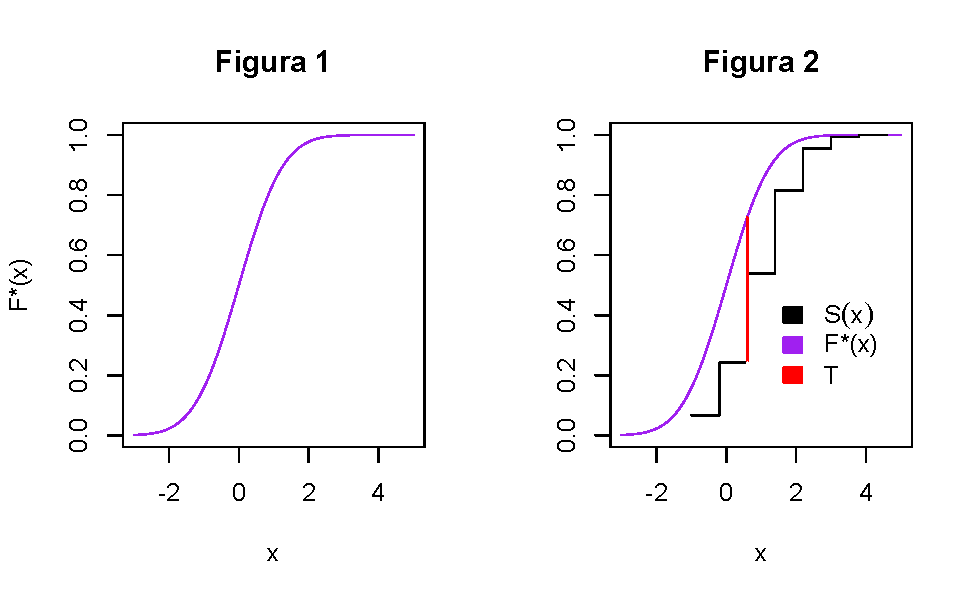
\includegraphics{_main_files/figure-latex/unnamed-chunk-53-1} \end{center}

Pero, ¿qué tipo de estadística de prueba podemos usar como medida de la diferencia entre \(S(x)\) y \(F^* (x)\)? Una de las medidas más simples imaginables es la mayor distancia entre los dos gráficos \(S(x)\) y \(F^*(x)\), medidos en dirección vertical. Ésta es la estadística sugerida por Kolmogorov (1993).
Es decir, si la \textbf{figura 1} proporciona \(F^*(x)\) y se extrae una muestra aleatoria de tamaño 5 de la población, la función de distribución empírica \(S(x)\) se puede dibujar en el mismo gráfico junto con \(F^ *(x)\), como se muestra en la figura 2.
Si \(F^*(x)\) y \(S(x)\) son como se indica, la distancia vertical máxima entre los dos gráficos se produce justo antes del tercer paso de \(S(x)\).
Esta distancia es de aproximadamente 0.5 en la \textbf{figura 2}; por lo tanto, el estadístico Kolmogorov T es igual a 0.5 en este caso.
Los valores grandes de \(T\) según lo determinado por la correspondiente tabla (Tabla de Cuantiles Kolmogorov) conducen a rechazar \(F^*(x)\) como una aproximación razonable a la función de distribución verdadera desconocida \(F(x)\).

La prueba de Kolmogorov puede preferirse a la prueba de Ji-Cuadrada para bondad del ajuste si el tamaño de la muestra es pequeño; la prueba de Kolmogorov es exacta incluso para muestras pequeñas, mientras que la prueba de Ji-cuadrada supone que el número de observaciones es lo suficientemente grande como para que la distribución de \(\chi^2\) proporcione una buena aproximación como la distribución del estadístico de prueba. Existe controversia sobre ¿qué prueba es la más ``poderosa''?, pero la sensación general parece ser que la prueba de Kolmogorov es probablemente más poderosa que la prueba de Ji-cuadrada en la mayoría de las situaciones que involucran datos ordinales.

\hypertarget{datos-15}{%
\section{Datos}\label{datos-15}}

Los datos consisten en una muestra aleatoria \(X_{1},X_{2},\ldots,X_{n}\) de tamaño \(n\) asociada con alguna función de distribución desconocida, denotada por \(F(x)\).

\hypertarget{supuestos-13}{%
\section{Supuestos}\label{supuestos-13}}

\begin{enumerate}
\def\labelenumi{\arabic{enumi})}
\tightlist
\item
  La muestra es una muestra aleatoria.
\end{enumerate}

\hypertarget{estaduxedstico-de-prueba-14}{%
\section{Estadístico de Prueba}\label{estaduxedstico-de-prueba-14}}

Sea \(S(x)\) la función de distribución empírica basada en la muestra aleatoria \(X_{1},X_{2},\ldots,X_{n}\). El estadístico de prueba es definido diferente para los 3 casos para las hipótesis correspondientes. Sea \(F^*(x)\) una función de distribución hipotética completamente especificada.

\hypertarget{caso-a-prueba-de-2-colas}{%
\subsection*{Caso A (Prueba de 2 colas)}\label{caso-a-prueba-de-2-colas}}


Sea el estadístico de prueba \(T\) la mayor distancia vertical entre \(S(x)\) y \(F^*(x)\)(denotado por sup o el supremo).

\[T=\underset{x}{sup}|F^*(x)-S(x)|\]

Esto se lee ``\(T\) es igual al supremo para todas las \(x\), del valor absoluto de la diferencia de \(F^*(x)-S(x)\)''

\hypertarget{caso-b-prueba-de-1-cola}{%
\subsection*{Caso B (Prueba de 1 cola)}\label{caso-b-prueba-de-1-cola}}


Denotamos el estadístico de prueba \(T^+\) la mayor distancia vertical alcanzada por \(F^*(x)\) sobre \(S(x)\).

\[T^+=\underset{x}{sup}[F^*(x)-S(x)] \]
Que es similar a \(T\), a excepción que solo vamos a considerar la mayor diferencia alcanzada por \(F^*(x)\) sobre la función \(S(x)\).

\hypertarget{caso-c-prueba-de-1-cola}{%
\subsection*{Caso C (Prueba de 1 cola)}\label{caso-c-prueba-de-1-cola}}


Denotamos el estadístico de prueba \(T^-\) la mayor distancia vertical alcanzada por \(S(x)\) sobre \(F^*(x)\).

\[T^-=\underset{x}{sup}[S(x)-F^*(x)] \]
Que es similar a \(T\), a excepción que solo vamos a considerar la mayor diferencia alcanzada por \(S(x)\) sobre la función \(F^*(x)\).

\hypertarget{hipuxf3tesis-14}{%
\section{Hipótesis}\label{hipuxf3tesis-14}}

\hypertarget{caso-a-prueba-de-2-colas-1}{%
\subsection*{Caso A (Prueba de 2 colas)}\label{caso-a-prueba-de-2-colas-1}}


\[\textbf{H}_0:\ F(x)=F^*(x) \ \ \ \ \forall \ \ x \ \ \  \mbox{de}\  \ -\infty \ \ \ \mbox{a} \  +\infty \]

\[vs\]

\[\textbf{H}_a: \ F(x) \neq F^*(x) \ \ \ \ \mbox{para al menos un  valor de} \   x.\]

\hypertarget{regla-de-decisiuxf3n-28}{%
\subsubsection*{Regla de decisión}\label{regla-de-decisiuxf3n-28}}


Rechazo \(H_0\) a un nivel de significancia \(\alpha\) si \(T>W\). Donde \(W\) es el cuantil \((1-\alpha)\), obtenido en la tabla correspondiente a nuestra prueba, para la prueba de 2 colas.

\hypertarget{caso-b-prueba-de-1-cola-1}{%
\subsection*{Caso B (Prueba de 1 cola)}\label{caso-b-prueba-de-1-cola-1}}


\[\textbf{H}_0: \ F(x) \geq F^*(x) \ \ \ \ \forall\ x\ \ \mbox{de} \ \ -\infty \  \ \  \mbox{a} \ \ +\infty\]

\[vs\]

\[Ha: \ F(x) < F^*(x) \ \ \ \ \mbox{para al menos un valor de} \  x.\]

\hypertarget{regla-de-decisiuxf3n-29}{%
\subsubsection*{Regla de decisión}\label{regla-de-decisiuxf3n-29}}


Rechazo \(H_0\) a un nivel de significancia \(\alpha\) si \(T^+>W\). Donde \(W\) es el cuantil \((1-\alpha)\),obtenido en la tabla correspondiente a nuestra prueba, para la prueba de 1 cola.

\hypertarget{caso-c-prueba-de-1-cola-1}{%
\subsection*{Caso C (Prueba de 1 cola)}\label{caso-c-prueba-de-1-cola-1}}


\[\textbf{H}_0:\ F(x) \leq F^*(x) \ \ \ \ \forall \ \ x \ \  \mbox{de} \  \ -\infty \ \  \mbox{a} \ \  +\infty\]

\[vs\]

\[\textbf{H}_a: \ F(x) > F^*(x) \ \ \ \ \mbox{para al menos un valor de} \  x.\]

\hypertarget{regla-de-decisiuxf3n-30}{%
\subsubsection*{Regla de decisión}\label{regla-de-decisiuxf3n-30}}


Rechazo \(H_0\) a un nivel de significancia \(\alpha\) si \(T^->W\). Donde \(W\) es el cuantil \((1-\alpha)\),obtenido en la tabla correspondiente a nuestra prueba, para la prueba de 1 cola.

Vamos a aplicar este conocimiento en un ejemplo:

\hypertarget{ejemplo-13}{%
\section{Ejemplo}\label{ejemplo-13}}

Una muestra aleatoria de tamaño 10, es obtenida:

\(X_{1}=0.621,\ \ X_{2}=0.503, \ \ X_{3}=0.203, \ X_{4}=0.477, \ X_{5}=0.710, \ X_{6}=0.581, \\ X_{7}=0.329, \ X_{8}=0.480, \  X_{9}=0.554, \ X_{10}=0.382\)

La hipótesis nula es que la función de distribución es una función de distribución uniforme.
La expresión matemática de función de distribución hipotética es:

\[
\textbf{F*(x)=} \left\{
\begin{array}{lcc}
0 & si & x < 0 \\
x & si & 0 \leq x < 1 \\
1 & si & 1 \leq x \\
\end{array}
\right.
\]

\textbf{Paso 1} Prueba a utilizar \textbf{Prueba de Bondad de Ajuste Kolmogorov}

\textbf{Paso 2} Planteamiento de Hipótesis

\[\textbf{H}_0: \ F(x)=F^*(x) \ \ \ \ \forall \ \ x \ \ \mbox{de} \ \ -\infty \ \  \mbox{a} \ \  +\infty\]

\[vs\]

\[\textbf{H}_a: \ F(x) \neq F^*(x) \ \ \ \ \mbox{para al menos un  valor de} \  x.\]

\begin{itemize}
\tightlist
\item
  Donde \textbf{F(x)} es la función de distribución desconocida común a las \(X_{i}s\) y \(F^*(x)\) se da por la expresión matemática.
\end{itemize}

\[
\textbf{F*(x)=} \left\{
\begin{array}{lcc}
0 & si & x < 0 \\
x & si & 0 \leq x < 1 \\
1 & si & 1 \leq x \\
\end{array}
\right.
\]

\textbf{Paso 3} Estadístico de Prueba

Calculamos el Estadístico de Prueba:

\[T=\underset{x}{sup}|F^*(x)-S(x)|\]
\[T=0.290\]

\textbf{Paso 4} Procedimiento completo para el cálculo del Estadístico de Prueba:
La siguiente tabla representa los cálculos para encontrar nuestro Estadístico de Prueba \(T\):

\(i\)

\(X(i)=x\)

\(F^*(x)\)

\(S_n\)

\(F^*(x)-S_n(x)\)

\(|F^*(x)-S_n(x)|\)

1

0.203

0.203

0.1

0.103

0.103

2

0.329

0.329

0.2

0.129

0.129

3

0.382

0.382

0.3

0.082

0.082

4

0.477

0.477

0.4

0.077

0.077

5

0.480

0.480

0.5

-0.020

0.020

6

0.503

0.503

0.6

-0.097

0.097

7

0.554

0.554

0.7

-0.146

0.146

8

0.581

0.581

0.8

-0.219

0.219

9

0.621

0.621

0.9

-0.279

0.279

10

0.710

0.710

1.0

-0.290

0.290

\textbf{Paso 5} Regla de Decisión

El cuantil \(W\) que acumula \(1-\alpha\) de probabilidad, usando \(\alpha\)=0.05 es \(W=0.409\), encontrado en las tablas correspondientes.

Tenemos que \(T<W\), entonces no rechazamos la hipotesis nula.

\textbf{Paso 6} Conclusión

Entonces podemos concluir que los datos siguen una distribución uniforme.

\hypertarget{ejemplo-en-r-studio-14}{%
\section{Ejemplo en R-Studio}\label{ejemplo-en-r-studio-14}}

Ahora haremos la réplica en R.

\begin{Shaded}
\begin{Highlighting}[]
\NormalTok{i }\OtherTok{=} \FunctionTok{c}\NormalTok{(}\DecValTok{1}\SpecialCharTok{:}\DecValTok{10}\NormalTok{) }\CommentTok{\#Representa el numero de nuestra muestra}
\NormalTok{x }\OtherTok{=} \FunctionTok{c}\NormalTok{(}\FloatTok{0.203}\NormalTok{,}\FloatTok{0.329}\NormalTok{,}\FloatTok{0.382}\NormalTok{,}\FloatTok{0.477}\NormalTok{,}\FloatTok{0.480}\NormalTok{,}\FloatTok{0.503}\NormalTok{,}\FloatTok{0.554}\NormalTok{,}\FloatTok{0.581}\NormalTok{,}\FloatTok{0.621}\NormalTok{, }\FloatTok{0.710}\NormalTok{) }\CommentTok{\#Los datos de la muestra}
\NormalTok{X\_i }\OtherTok{=} \FunctionTok{sort}\NormalTok{(x) }\CommentTok{\#ordena nuestros datos}
\NormalTok{F\_}\OtherTok{=}\FunctionTok{c}\NormalTok{(}\FloatTok{0.203}\NormalTok{,}\FloatTok{0.329}\NormalTok{,}\FloatTok{0.382}\NormalTok{,}\FloatTok{0.477}\NormalTok{,}\FloatTok{0.480}\NormalTok{,}\FloatTok{0.503}\NormalTok{,}\FloatTok{0.554}\NormalTok{,}\FloatTok{0.581}\NormalTok{,}\FloatTok{0.621}\NormalTok{, }\FloatTok{0.710}\NormalTok{)}
\NormalTok{Sn}\OtherTok{=}\FunctionTok{c}\NormalTok{(}\DecValTok{1}\SpecialCharTok{/}\DecValTok{10}\NormalTok{,}\DecValTok{2}\SpecialCharTok{/}\DecValTok{10}\NormalTok{,}\DecValTok{3}\SpecialCharTok{/}\DecValTok{10}\NormalTok{,}\DecValTok{4}\SpecialCharTok{/}\DecValTok{10}\NormalTok{,}\DecValTok{5}\SpecialCharTok{/}\DecValTok{10}\NormalTok{,}\DecValTok{6}\SpecialCharTok{/}\DecValTok{10}\NormalTok{,}\DecValTok{7}\SpecialCharTok{/}\DecValTok{10}\NormalTok{,}\DecValTok{8}\SpecialCharTok{/}\DecValTok{10}\NormalTok{,}\DecValTok{9}\SpecialCharTok{/}\DecValTok{10}\NormalTok{,}\DecValTok{1}\NormalTok{)}
\NormalTok{Tabla }\OtherTok{=} \FunctionTok{cbind}\NormalTok{(i,}\AttributeTok{X\_i=}\NormalTok{X\_i,F\_,Sn,}\StringTok{"|F\_{-}Sn|"}\OtherTok{=}\FunctionTok{abs}\NormalTok{(F\_}\SpecialCharTok{{-}}\NormalTok{Sn))}
\NormalTok{Tabla}
\end{Highlighting}
\end{Shaded}

\begin{verbatim}
       i   X_i    F_  Sn |F_-Sn|
 [1,]  1 0.203 0.203 0.1   0.103
 [2,]  2 0.329 0.329 0.2   0.129
 [3,]  3 0.382 0.382 0.3   0.082
 [4,]  4 0.477 0.477 0.4   0.077
 [5,]  5 0.480 0.480 0.5   0.020
 [6,]  6 0.503 0.503 0.6   0.097
 [7,]  7 0.554 0.554 0.7   0.146
 [8,]  8 0.581 0.581 0.8   0.219
 [9,]  9 0.621 0.621 0.9   0.279
[10,] 10 0.710 0.710 1.0   0.290
\end{verbatim}

\begin{Shaded}
\begin{Highlighting}[]
\NormalTok{EstdPrueba }\OtherTok{=} \FunctionTok{max}\NormalTok{(Tabla [,}\DecValTok{5}\NormalTok{])}
\NormalTok{EstdPrueba}
\end{Highlighting}
\end{Shaded}

\begin{verbatim}
[1] 0.29
\end{verbatim}

Observamos que la estadística de prueba tiene un valor de 0.29. El cuantil W que acumula \(1-\alpha\) de probabilidad, usando \(\alpha=0.05\) es W = 0.409, encontrado en las tablas correspondientes. Por lo tanto tenemos que \(T_1 < W\), entonces no rechazamos la hipotesis nula.y su correspondiente p-value es mucho mayor a 0.05, por lo tanto con \(\alpha=5\%\) no rechazaremos \(H_0\) y concluimos no existe evidencia suficiente para suponer que la distribución de la muestra no es uniforme en el intervalo (0,1).

Ahora haremos la prueba usando la función \textbf{``ks.test''} de R.

\begin{Shaded}
\begin{Highlighting}[]
\CommentTok{\#Prueba}
\FunctionTok{ks.test}\NormalTok{(X\_i,Sn)}
\end{Highlighting}
\end{Shaded}

\begin{verbatim}
    Two-sample Kolmogorov-Smirnov test

data:  X_i and Sn
D = 0.3, p-value = 0.7869
alternative hypothesis: two-sided
\end{verbatim}

\hypertarget{otro-ejemplo-en-r}{%
\section{Otro ejemplo en R}\label{otro-ejemplo-en-r}}

Se mencionó que uno de los usos de estas pruebas es para validar el supuesto de normalidad en los modelos de regresión lineal. Veremos ahora un ejemplo en donde los datos a los que se aplica la prueba de bondad de ajuste son los residuales de una regresión lineal simple.

La base de datos \textbf{``Loblolly''} en R, contiene información sobre tres características de arboles de pino originarios del sudeste de Estados Unidos. Al ajustar un modelo de regresión lineal simple entre \(X="edad"\) y \(Y="altura"\), deseamos probar con un nivel de significancia del \(1\%\) que los residuales estandarizados se distribuyen normal estándar.

\begin{Shaded}
\begin{Highlighting}[]
\NormalTok{m1}\OtherTok{=}\FunctionTok{lm}\NormalTok{(Loblolly}\SpecialCharTok{$}\NormalTok{height}\SpecialCharTok{\textasciitilde{}}\NormalTok{Loblolly}\SpecialCharTok{$}\NormalTok{age)}
\NormalTok{x}\OtherTok{=}\FunctionTok{rstandard}\NormalTok{(m1)}

\FunctionTok{ks.test}\NormalTok{(x,}\StringTok{"pnorm"}\NormalTok{,}\DecValTok{0}\NormalTok{,}\DecValTok{1}\NormalTok{)}
\end{Highlighting}
\end{Shaded}

\begin{verbatim}
    One-sample Kolmogorov-Smirnov test

data:  x
D = 0.10804, p-value = 0.2613
alternative hypothesis: two-sided
\end{verbatim}

Observamos que la estadística de prueba tiene un valor de 0.10804 y su correspondiente \(p-value\) es \(26.13\%\), por lo tanto con \(\alpha=5\%\) no rechazaremos \(H_0\) y concluimos no existe evidencia suficiente para suponer que la distribución de la muestra no es normal(0,1).

\hypertarget{prueba-kolmogorov-smirnov}{%
\chapter{Prueba Kolmogorov-Smirnov}\label{prueba-kolmogorov-smirnov}}

En ejercicios prácticos es muy difícil conocer la distribución de una muestra aleatoria, generalmente
sólo se tiene la información; ésta hay que procesarla para averiguar si sigue una determinada distribución probabilística, en un primer intento se ajustó mediante la prueba de la Ji-cuadrada, sin embargo, al ser una de las pruebas más sencillas su \textbf{``potencia''} al estimar una determinada distribución es baja, es por ello, que se idearon otros métodos y uno de ello es la Prueba de Kolmogorov-Smirnov.

La prueba de Kolmogorov presenta la ventaja de que los datos no deben ser categorizadas para poder realizar estimaciones en su distribución. Al igual que en la prueba de la Ji-Cuadrada, Kolmogorov-Smirnov trabaja con una distribución \(F^*(x)\) totalmente especificada, es decir, se debe de tener sospecha de que la muestra aleatoria siga una determinada distribución. De esta manera el objeto de estudio es una muestra \(X_{1},\ldots,X_{n}\) de variables aleatorias idénticamente distribuidas, las cuales siguen una distribución desconocida \(F(X)\) y se tiene la sospecha de que la muestra sigue una distribución conocida \(F^*(x)\).

Para probar la suposición de la distribución \(F^*(x)\) se realiza la siguiente contraste:

\hypertarget{hipuxf3tesis-15}{%
\section{Hipótesis}\label{hipuxf3tesis-15}}

\hypertarget{caso-a-prueba-de-2-colas-2}{%
\subsection{Caso A (Prueba de 2 colas)}\label{caso-a-prueba-de-2-colas-2}}

Solo será este caso

\[\textbf{H}_0: \ F(x)=F^*(x) \ \ \ \ \forall \ \ x\ \  \mbox{de} \ \ -\infty \ \  \mbox{a} \ \  +\infty\]

\[vs\]

\[\textbf{H}_a: \ F(x) \neq F^*(x) \ \ \ \ \mbox{para al menos un valor de} \  x.\]

\hypertarget{regla-de-decisiuxf3n-31}{%
\subsubsection*{Regla de decisión}\label{regla-de-decisiuxf3n-31}}


Rechazo \(H_0\) a un nivel de significancia \(\alpha\) si \(D_{n}>W\). Donde \(W\) es el cuantil \((1-\alpha)\), obtenido en la tabla correspondiente a nuestra prueba O para la prueba de 2 colas en las tablas de Kolmogorov.

\textbf{Donde} \(F^*(x)\) es una distribución completamente conocida, es decir además de conocer a la familia que pertenece también se conocen sus parámetros.

Lo que se busca es poder medir las distancia entre \(F(x)\), la distribución desconocida, con
los datos que siguen la función de distribución propuesta y completamente conocida \(F^*(x)\).
Sin embargo, \(F(x)\) al ser desconocida se recurre a la construcción de una distribución empírica
la cual se define como:

\[S_{n}(x)=\frac{ \sum_{i=1}^{n}número\ de\ valores\ muestrales\ \leq x}{n}\]

Es decir, la función empírica mide el número de elementos menores o iguales a la observación
\(X\), puede observarse que en el caso continuo, al no haber \textbf{``empates''} la función empírica puede
ser vista como:

\[S_{n}(x)=\frac{i}{n} \ \ \ i=1,\ldots,n\]

Al tener una distribución desconocida \(F(x)\), la función empírica \(S_{n}(x)\) puede ser usada
como un estimador insesgado de \(F(x)\) pues:

\[\mathbb{E}(S_{n}(x))=F(x)\]
La función empírica es de gran importancia ya que gracias al teorema de \textbf{Glivenko-Cantelli}
se sabe que cuando el tamaño de la muestra tiende a infinito cualquier distribución empírica
se aproxima a la distribución real de los datos, la cual, es una distribución completamente especificada. El teorema de \textbf{Glivenko-Cantelli}, menciona que al calcular las diferencias de la distribución real y la empírica éstas son cero en cada observación dada, el teorema que se enuncia como:

Sea \(X_{1},\ldots,X_{n}\) una muestra aleatoria de distribución \(F(x)\) desconocida y sea \(S_{n}(x)\) la función empírica entonces:

\[\underset{x}{sup} \ |\ S_{n}(x)-F(x) \ | \ \longrightarrow \ 0\]

Es decir, conforme mayor sea el tamaño de la muestra, \(S_{n}(x)\) reproduce la verdadera
distribución. De esta manera se establece el estadístico de Prueba \(Dn\), el cual no depende de ningún
parámetro desconocido, ya que engloba a la distribución empírica y a la distribución propuesta:

\[D_{n}=\underset{x}{sup} \ | \ S_{n}(x)-F^*(x) \ |=max \  \{ \ max \{ \  S_{n}(X_{i-1})-F^*(X_{i}) \ \},max \{ \  S_{n}(X_{i})-F^*(X_{i}) \ \} \ \} \ \  \ \forall \ i\]
y \[D_{n}= \ \underset{x}{sup} \ | \ S_{n}(x)-F^*(x) \ |=max \ \{ \  D^+,D^- \ \}\]

Donde:

\[D^+= max \ \{ \  S_{n}(X_{i})-F^*(X_{i}) \ \}\]
\[D^-= max \  \{ \ S_{n}(X_{i-1})-F^*(X_{i}) \ \}\]

Finalmente, se observa que si \(H_0\) es cierta si \(D_{n} \longrightarrow \ 0\) ya que las diferencias entre la diferencias entre la función empírica y la propuestas son mínimas, lo que cumple con el \textbf{Teorema de Glivenko-Cantelli} ; por lo que hay evidencia para rechazar \(H_0\) cuando \(D_{n} > W\) Donde \(W\) es el cuantil que acumula el \(1- \alpha\) de probabilidad de la distribución asociada a \(D_{n}\) la cual puede obtenerse de la tablas correspondientes la cual muestra los cuantiles de la distribución
Kolmogorov-Smirnov o la Tabla Kolmogorov para 2 colas.

\hypertarget{ejemplo-14}{%
\section{Ejemplo}\label{ejemplo-14}}

Dada la siguiente muestra

\[0.6379 \ \ 1.5299 \ \ 0.35005 \ \ 2.0505 \ \ 2.1906 \ \ 0.3459 \ \ 2.3214 \ \ 0.3128\]
\[ 0.65482.4373 \ \ 1.803 \ \ 2.3674 \ \ 1.2716 \ \ 0.2566 \ \ 0.2513\]

Se desea hacer el siguiente contraste:

\[\textbf{H}_0: \ \mbox{Los datos} \  \sim  \ LogN(0,1)\]

\[vs\]

\[\textbf{H}_a: \ \mbox{Los datos} \ \ \nsim \ LogN(0,1)\]

Realice la prueba de Kolmogorov-Smirnov al 5\% de significancia.

\textbf{Paso 1} Prueba a utilizar \textbf{Prueba de Bondad de Ajuste Kolmogorov-Smirnov}

\textbf{Paso 2} Planteamiento de Hipótesis

\[\textbf{H}_0: \ \mbox{Los datos} \ \sim  \ LogN(0,1)\]

\[vs\]

\[\textbf{H}_a: \ \mbox{Los datos} \  \nsim \  LogN(0,1)\]

\textbf{Paso 3} Estadístico de Prueba:

\[D_{n}=\underset{x}{sup} \ | \ S_{n}(x)-F^*(x) \ |=max \ \{\ D^+,D^- \ \}\]

\textbf{Paso 4} Procedimiento completo para el cálculo del Estadístico de Prueba:

\begin{enumerate}
\def\labelenumi{\arabic{enumi})}
\item
  Se procede a ordenar nuestras observaciones de menor a mayor.
\item
  Se calcula la función empírica, como no tenemos ningún valor repetido:
\end{enumerate}

\[S_{n}= \frac{i}{n}=\frac{1}{15},\frac{2}{15}, \ldots, 1.\]

\begin{enumerate}
\def\labelenumi{\arabic{enumi})}
\setcounter{enumi}{2}
\item
  Se calcula la función empírica menos un valor, es decir,\}
  \[S_{n}= \frac{i-1}{n}=\frac{0}{15},\frac{1}{15}, \ldots, \frac{14}{15}.\]
\item
  Se calcula la distribución conocida, es decir, \(F^*(x) \ \ \  LogN(0,1)\)
\item
  Se calcula \(D^+\) que es el resultado de la resta de la distribución conocida menos la distribución empírica, es decir:
\end{enumerate}

\[D^+= max \ \{\ S_{n}(X_{i})-F^*(X_{i}) \ \}\]

\begin{enumerate}
\def\labelenumi{\arabic{enumi})}
\setcounter{enumi}{5}
\tightlist
\item
  Se calcula \(D^-\) que es el resultado de la resta de la distribución empírica menos uno menos la distribución conocida, es decir:
\end{enumerate}

\[D^-= max \ \{\ S_{n}(X_{i-1})-F^*(X_{i}) \ \}\]

\begin{enumerate}
\def\labelenumi{\arabic{enumi})}
\setcounter{enumi}{6}
\tightlist
\item
  Finalmente realizada la tabla, se calcula el máximo de las columnas \(D^+\) y \(D^-\) de ésta manera, se tiene la siguiente tabla:
\end{enumerate}

\(i\)

\(X\)

\(X_i\)

\(S_n(X_i)\)

\(S_n(X_{i-1})\)

\(F^*(X_i)\)

\(D^+=S_n(X_i)-F^*(X_i)\)

\(D^-=S_n(X_{i-1})-F^*(X_i)\)

1

0.63790

0.25130

0.0666667

0.0000000

0.0836

-0.0169

-0.0836

2

1.52990

0.25660

0.1333333

0.0666667

0.0869

0.0464

-0.0202

3

0.35005

0.31280

0.2000000

0.1333333

0.1226

0.0774

0.0107

4

2.05050

0.34590

0.2666667

0.2000000

0.1442

0.1224

0.0558

5

2.19060

0.35005

0.3333333

0.2666667

0.1472

0.1861

0.1194

6

0.34590

0.63790

0.4000000

0.3333333

0.3265

0.0735

0.0068

7

2.32140

0.65480

0.4666667

0.4000000

0.3360

0.1306

0.0640

8

0.31280

1.27160

0.5333333

0.4666667

0.5949

-0.0615

-0.1282

9

0.65480

1.52990

0.6000000

0.5333333

0.6647

-0.0647

-0.1313

10

2.43730

1.80300

0.6666667

0.6000000

0.7222

-0.0555

-0.1222

11

1.80300

2.05050

0.7333333

0.6666667

0.7636

-0.0302

-0.0969

12

2.36740

2.19060

0.8000000

0.7333333

0.7835

0.0165

-0.0501

13

1.27160

2.32140

0.8666667

0.8000000

0.8002

0.0664

-0.0002

14

0.25660

2.36740

0.9333333

0.8666667

0.8056

0.1277

0.0610

15

0.25130

2.43730

1.0000000

0.9333333

0.8135

0.1865

0.1198

\begin{enumerate}
\def\labelenumi{\arabic{enumi})}
\setcounter{enumi}{7}
\tightlist
\item
  Entonces
\end{enumerate}

\[ D^+= max\ \{\ S_{n}(X_{i})-F^*(X_{i}) \ \}= 0.1865 \ \ \ \ y\ \ \ \ D^-= max\ \{\ S_{n}(X_{i-1})-F^*(X_{i})\ \}=0.1198\]
Por lo tanto:

\[D_{n}=\underset{x}{sup}\ | \ S_{n}(x)-F^*(x) \ |=max \ \{ \ D^+,D^- \ \}=max \ \{ \  0.1865,0.1198 \ \}=0.1865\]

\textbf{Paso 5} Regla de Decisión

Este último resultado se compara con la tabla de valores críticos de la Tabla Kolmogorov-Smirnov, para un nivel de significancia \(\alpha\) = 0.05
\(W_{0.05}\)=0.338, de esta manera se tiene que 0.338 = \(W_{0.05} > D_{n}\) = 0.1865, como el estadístico \(W_{0.05}\) es mayor a comparación de \(D_{n}\)=0.1865.
No Rechazamos \(H_0\).

\textbf{Paso 6} Conclusión

Se acepta la prueba de lognormalidad con media 1 y varianza 0, con un nivel de significancia \(\alpha\) = 0.05. Es decir, Los datos se distribuyen \(LogN(0,1)\).

\begin{Shaded}
\begin{Highlighting}[]
\NormalTok{i}\OtherTok{=} \DecValTok{1}\SpecialCharTok{:}\DecValTok{15}
\NormalTok{X}\OtherTok{=} \FunctionTok{c}\NormalTok{(}\FloatTok{0.6379}\NormalTok{,}\FloatTok{1.5299}\NormalTok{,}\FloatTok{0.35005}\NormalTok{,}\FloatTok{2.0505}\NormalTok{,}\FloatTok{2.1906}\NormalTok{,}\FloatTok{0.3459}\NormalTok{,}\FloatTok{2.3214}\NormalTok{,}\FloatTok{0.3128}\NormalTok{,}\FloatTok{0.6548}\NormalTok{,}\FloatTok{2.4373}\NormalTok{,}
               \FloatTok{1.803}\NormalTok{,}\FloatTok{2.3674}\NormalTok{,}\FloatTok{1.2716}\NormalTok{,}\FloatTok{0.2566}\NormalTok{,}\FloatTok{0.2513}\NormalTok{)}
\NormalTok{X\_i}\OtherTok{=}\FunctionTok{c}\NormalTok{(}\FloatTok{0.25130}\NormalTok{,}\FloatTok{0.25660}\NormalTok{,}\FloatTok{0.31280}\NormalTok{, }\FloatTok{0.34590}\NormalTok{,}\FloatTok{0.35005}\NormalTok{,}\FloatTok{0.63790}\NormalTok{, }\FloatTok{0.65480}\NormalTok{, }\FloatTok{1.27160}\NormalTok{, }
               \FloatTok{1.52990}\NormalTok{,}\FloatTok{1.80300}\NormalTok{, }\FloatTok{2.05050}\NormalTok{, }\FloatTok{2.19060}\NormalTok{, }\FloatTok{2.32140}\NormalTok{, }\FloatTok{2.36740}\NormalTok{,}\FloatTok{2.43730}\NormalTok{)}

\NormalTok{Sn}\OtherTok{=}\FunctionTok{c}\NormalTok{(}\DecValTok{1}\SpecialCharTok{/}\DecValTok{15}\NormalTok{,}\DecValTok{2}\SpecialCharTok{/}\DecValTok{15}\NormalTok{,}\DecValTok{3}\SpecialCharTok{/}\DecValTok{15}\NormalTok{,}\DecValTok{4}\SpecialCharTok{/}\DecValTok{15}\NormalTok{,}\DecValTok{5}\SpecialCharTok{/}\DecValTok{15}\NormalTok{,}\DecValTok{6}\SpecialCharTok{/}\DecValTok{15}\NormalTok{,}\DecValTok{7}\SpecialCharTok{/}\DecValTok{15}\NormalTok{,}\DecValTok{8}\SpecialCharTok{/}\DecValTok{15}\NormalTok{,}\DecValTok{9}\SpecialCharTok{/}\DecValTok{15}\NormalTok{,}\DecValTok{10}\SpecialCharTok{/}\DecValTok{15}\NormalTok{,}\DecValTok{11}\SpecialCharTok{/}\DecValTok{15}\NormalTok{,}\DecValTok{12}\SpecialCharTok{/}\DecValTok{15}\NormalTok{,}\DecValTok{13}\SpecialCharTok{/}\DecValTok{15}\NormalTok{,}\DecValTok{14}\SpecialCharTok{/}\DecValTok{15}\NormalTok{,}\DecValTok{1}\NormalTok{)}
\NormalTok{Sn\_1}\OtherTok{=}\FunctionTok{c}\NormalTok{(}\DecValTok{0}\SpecialCharTok{/}\DecValTok{15}\NormalTok{,}\DecValTok{1}\SpecialCharTok{/}\DecValTok{15}\NormalTok{,}\DecValTok{2}\SpecialCharTok{/}\DecValTok{15}\NormalTok{,}\DecValTok{3}\SpecialCharTok{/}\DecValTok{15}\NormalTok{,}\DecValTok{4}\SpecialCharTok{/}\DecValTok{15}\NormalTok{,}\DecValTok{5}\SpecialCharTok{/}\DecValTok{15}\NormalTok{,}\DecValTok{6}\SpecialCharTok{/}\DecValTok{15}\NormalTok{,}\DecValTok{7}\SpecialCharTok{/}\DecValTok{15}\NormalTok{,}\DecValTok{8}\SpecialCharTok{/}\DecValTok{15}\NormalTok{,}\DecValTok{9}\SpecialCharTok{/}\DecValTok{15}\NormalTok{,}\DecValTok{10}\SpecialCharTok{/}\DecValTok{15}\NormalTok{,}\DecValTok{11}\SpecialCharTok{/}\DecValTok{15}\NormalTok{,}\DecValTok{12}\SpecialCharTok{/}\DecValTok{15}\NormalTok{,}\DecValTok{13}\SpecialCharTok{/}\DecValTok{15}\NormalTok{,}\DecValTok{14}\SpecialCharTok{/}\DecValTok{15}\NormalTok{)}
\NormalTok{F\_}\OtherTok{=}\FunctionTok{c}\NormalTok{(}\FloatTok{0.0836}\NormalTok{,}\FloatTok{0.0869}\NormalTok{,}\FloatTok{0.1226}\NormalTok{,}\FloatTok{0.1442}\NormalTok{,}\FloatTok{0.1472}\NormalTok{,}\FloatTok{0.3265}\NormalTok{,}\FloatTok{0.3360}\NormalTok{,}\FloatTok{0.5949}\NormalTok{,}
                    \FloatTok{0.6647}\NormalTok{,}\FloatTok{0.7222}\NormalTok{,}\FloatTok{0.7636}\NormalTok{,}\FloatTok{0.7835}\NormalTok{,}\FloatTok{0.8002}\NormalTok{,}\FloatTok{0.8056}\NormalTok{,}\FloatTok{0.8135}\NormalTok{)}
\NormalTok{D\_mas}\OtherTok{=}\FunctionTok{c}\NormalTok{(}\SpecialCharTok{{-}}\FloatTok{0.0169}\NormalTok{,}\FloatTok{0.0464}\NormalTok{,}\FloatTok{0.0774}\NormalTok{,}\FloatTok{0.1224}\NormalTok{,}\FloatTok{0.1861}\NormalTok{,}\FloatTok{0.0735}\NormalTok{,}\FloatTok{0.1306}\NormalTok{,}\SpecialCharTok{{-}}\FloatTok{0.0615}\NormalTok{,}\SpecialCharTok{{-}}\FloatTok{0.0647}\NormalTok{,}\SpecialCharTok{{-}}\FloatTok{0.0555}\NormalTok{,}
                \SpecialCharTok{{-}}\FloatTok{0.0302}\NormalTok{,}\FloatTok{0.0165}\NormalTok{,}\FloatTok{0.0664}\NormalTok{,}\FloatTok{0.1277}\NormalTok{,}\FloatTok{0.1865}\NormalTok{)}
\NormalTok{D\_menos}\OtherTok{=}\FunctionTok{c}\NormalTok{(}\SpecialCharTok{{-}}\FloatTok{0.0836}\NormalTok{,}\SpecialCharTok{{-}}\FloatTok{0.0202}\NormalTok{,}\FloatTok{0.0107}\NormalTok{,}\FloatTok{0.0558}\NormalTok{,}\FloatTok{0.1194}\NormalTok{,}\FloatTok{0.0068}\NormalTok{,}\FloatTok{0.0640}\NormalTok{,}\SpecialCharTok{{-}}\FloatTok{0.1282}\NormalTok{,}
          \SpecialCharTok{{-}}\FloatTok{0.1313}\NormalTok{,}\SpecialCharTok{{-}}\FloatTok{0.1222}\NormalTok{,}\SpecialCharTok{{-}}\FloatTok{0.0969}\NormalTok{,}\SpecialCharTok{{-}}\FloatTok{0.0501}\NormalTok{,}\SpecialCharTok{{-}}\FloatTok{0.0002}\NormalTok{,}\FloatTok{0.0610}\NormalTok{,}\FloatTok{0.1198}\NormalTok{)}

\NormalTok{Tabla}\OtherTok{=}\FunctionTok{cbind}\NormalTok{(i,X\_i,Sn,Sn\_1,F\_,D\_mas,D\_menos)                                                                                                                                                      }
\NormalTok{Tabla}
\end{Highlighting}
\end{Shaded}

\begin{verbatim}
       i     X_i         Sn       Sn_1     F_   D_mas D_menos
 [1,]  1 0.25130 0.06666667 0.00000000 0.0836 -0.0169 -0.0836
 [2,]  2 0.25660 0.13333333 0.06666667 0.0869  0.0464 -0.0202
 [3,]  3 0.31280 0.20000000 0.13333333 0.1226  0.0774  0.0107
 [4,]  4 0.34590 0.26666667 0.20000000 0.1442  0.1224  0.0558
 [5,]  5 0.35005 0.33333333 0.26666667 0.1472  0.1861  0.1194
 [6,]  6 0.63790 0.40000000 0.33333333 0.3265  0.0735  0.0068
 [7,]  7 0.65480 0.46666667 0.40000000 0.3360  0.1306  0.0640
 [8,]  8 1.27160 0.53333333 0.46666667 0.5949 -0.0615 -0.1282
 [9,]  9 1.52990 0.60000000 0.53333333 0.6647 -0.0647 -0.1313
[10,] 10 1.80300 0.66666667 0.60000000 0.7222 -0.0555 -0.1222
[11,] 11 2.05050 0.73333333 0.66666667 0.7636 -0.0302 -0.0969
[12,] 12 2.19060 0.80000000 0.73333333 0.7835  0.0165 -0.0501
[13,] 13 2.32140 0.86666667 0.80000000 0.8002  0.0664 -0.0002
[14,] 14 2.36740 0.93333333 0.86666667 0.8056  0.1277  0.0610
[15,] 15 2.43730 1.00000000 0.93333333 0.8135  0.1865  0.1198
\end{verbatim}

\begin{Shaded}
\begin{Highlighting}[]
\NormalTok{EstdPrueba }\OtherTok{=} \FunctionTok{max}\NormalTok{(D\_mas,D\_menos)}
\NormalTok{EstdPrueba}
\end{Highlighting}
\end{Shaded}

\begin{verbatim}
[1] 0.1865
\end{verbatim}

Por lo tanto:

\[D_{n}=\underset{x}{sup} \ | \ S_{n}(x)-F^*(x)\ |=max\ \{\ D^+,D^- \ \}=max \ \{ \ 0.1865,0.1198 \ \}=0.1865\]

Lo comparamos con la tabla de valores críticos de la \textbf{Tabla Kolmogorov-Smirnov}, para un nivel de significancia \(\alpha\) = 0.05
\(W_{0.05}\)=0.338, de esta manera se tiene que 0.338 = \(W_{0.05} > D_{n}\) = 0.1865, como el estadístico \(W_{0.05}\) es mayor a comparación de \(D_{n}\)=0.1865.
No Rechazamos \(H_0\).

Podemos concluir aceptando la prueba de lognormalidad con media 1 y varianza 0, con un nivel de significancia \(\alpha\) = 0.05. Es decir, Los datos se distribuyen \(LogN(0,1)\).

\begin{Shaded}
\begin{Highlighting}[]
\CommentTok{\#Ahora podemos utilizar la prueba en R}
\FunctionTok{ks.test}\NormalTok{(F\_,Sn,}\AttributeTok{alternative =} \StringTok{"two.sided"}\NormalTok{)}
\end{Highlighting}
\end{Shaded}

\begin{verbatim}
    Two-sample Kolmogorov-Smirnov test

data:  F_ and Sn
D = 0.2, p-value = 0.9383
alternative hypothesis: two-sided
\end{verbatim}

\hypertarget{prueba-lilliefors-para-normalidad}{%
\chapter{Prueba Lilliefors para Normalidad}\label{prueba-lilliefors-para-normalidad}}

La prueba de bondad de ajuste de Kolmogorov presentada anteriormente es una buena prueba para ver si una muestra aleatoria tiene alguna función de distribución especificada. La prueba de Kolmogorov está diseñada para usarse solo cuando la función de distribución hipotética está completamente especificada, es decir, cuando no hay parámetros desconocidos que deben estimarse a partir de la muestra.
La prueba de bondad de ajuste Ji-cuadrada es lo suficientemente flexible como para permitir que algunos parámetros se estimen a partir de los datos.Simplemente se resta un grado de libertad para cada parámetro estimado descrita anteriormente.

Sin embargo, la prueba de Ji-cuadrada requiere que los datos se agrupen, y dicha agrupación de datos suele ser arbitraria. Además, la distribución del estadístico de prueba se conoce solo aproximadamente, y a veces el poder de la prueba de Ji-cuadrada no es muy bueno. Por estas razones, se buscan otras pruebas de bondad de ajuste, especialmente para distribuciones probadas con frecuencia.

La prueba de Kolmogorov se ha modificado para permitir su uso en varias situaciones en las que los parámetros se estiman a partir de los datos. En realidad, el estadístico de prueba permanece sin cambios, pero se utilizan diferentes tablas de valores críticos. Estas tablas ya no son las mismas para todas las distribuciones; cambian de una distribución hipotética a otra. La prueba sigue siendo una prueba no paramétrica porque la validez de la prueba (el nivel de \(\alpha\)) no depende de supuestos no probados con respecto a la distribución de la población; en cambio, la forma de distribución de la población es la hipótesis que se está probando.

La primera modificación a la prueba de Kolmogorov es para probar la hipótesis compuesta de la normalidad. Es decir, la hipótesis nula establece que la población es una de la familia de distribuciones normales sin especificar la media o la varianza de la distribución normal. Ésta prueba fue presentada por primera vez por Hubert Lilliefors (1967). Una característica interesante de esta prueba es que este es uno de los primeros casos en que el compilador se utilizó para generar números aleatorios con el fin de obtener estimaciones precisas de los verdaderos cuantiles de la distribución exacta del estadístico de la prueba y además, aproximar a los parámetros a través del uso de los estimadores puntuales.

\hypertarget{datos-16}{%
\section{Datos}\label{datos-16}}

Los datos consisten en una muestra aleatoria \(X_{1},X_{2},\ldots,X_{n}\) de tamaño \(n\) asociada con alguna función de distribución desconocida, denotada por \(F(x)\).

Calculando la media muestral

\[\overline{X}=\frac{1}{n}\sum_{i=1}^{n}X_{i}\]

para usarla como una estimación puntual de \(\mu\)

y calculando como una estimación de \(\sigma\)

\[s=\sqrt{\frac{1}{n-1}\sum_{i=1}^{n}(X_{i}-\overline{X})^2}\]

Después calcularemos los valores de muestra ``normalizados'' \(Z_{i}\) definidos por:

\[Z_{i}=\frac{X_{i}-\overline{X}}{s} \ \ \ \ i=1,2,\ldots,n\]

El estadístico de prueba se calcula a partir de \(Z_{i}s\) en lugar de a partir de la muestra aleatoria. original

\hypertarget{supuestos-14}{%
\section{Supuestos}\label{supuestos-14}}

\begin{enumerate}
\def\labelenumi{\arabic{enumi})}
\tightlist
\item
  La muestra es una muestra aleatoria.
\end{enumerate}

\hypertarget{hipuxf3tesis-16}{%
\section{Hipótesis}\label{hipuxf3tesis-16}}

\[\textbf{H}_0: \ \mbox{La muestra aleatoria proviene de una población con distribución normal,}\]
\[\mbox{con media y desviación estándar desconocidas.}\]
\[vs\]

\[\textbf{H}_a: \ \mbox{La función de distribución de las} \ \ X_{i}s \ \  \mbox{no es normal.}\]

\hypertarget{estaduxedstico-de-prueba-15}{%
\section{Estadístico de Prueba}\label{estaduxedstico-de-prueba-15}}

Normalmente, el estadístico de prueba es el mismo para la prueba de Kolmogorov de dos colas, definida como la distancia vertical máxima entre la función de distribución empírica de \(X_{i}s\) y la función de distribución normal con media \(\mu=\overline{X}\) y desviación estándar \(\sigma=s\).
Sin embargo, el siguiente método para calcular el estadístico de prueba es un poco más fácil, ya que es equivalente al método indicado. Es decir, el cálculo del estadístico \(T_{1}\) será en función de la \(Z_{i}s\).

\[T_{1}=\underset{x}{sup}|F^*(x)-S(x)|\]

\hypertarget{regla-de-decisiuxf3n-32}{%
\subsubsection*{Regla de Decisión}\label{regla-de-decisiuxf3n-32}}


Rechazo \(H_0\) a un nivel de significancia \(\alpha\) si \(T_{1}> W_{1-\alpha}\) donde \(W_{1-\alpha}\) es el cuantil obtenido en las tablas correspondientes a nuestra prueba.

\hypertarget{ejemplo-15}{%
\section{Ejemplo}\label{ejemplo-15}}

Los siguientes datos, corresponden a una muestra aleatoria en la que mide la pérdida y ganancia de peso en \(KG\) de un grupo después de vacaciones.

\[0.6822,\ 3.994,\ -0.9705,\ -0.5575,\ -2.1532,\ 0.0829,\ 2.9224,\ 0.2425\]
\[-0.4962,\ -0.1621,\ 0.449,\ -0.8827,\ -0.8368,\ -1.5805,\ 0.386.\]

Se desea probar si los datos provienen de una distribución normal con \(\mu\) y \(\sigma\) desconocidas.
Realizar la prueba a un nivel de significancia del \(95\%.\)

\textbf{Paso 1} Prueba a utilizar \textbf{Prueba de Bondad de Ajuste Lilliefors para Normalidad}

\textbf{Paso 2} Planteamiento de Hipótesis

\[\textbf{H}_0: \ \mbox{La muestra} \ \ \sim \ \  N(\mu,\sigma^2).\]
\[vs\]

\[\textbf{H}_a: \ \mbox{La muestra}  \ \nsim \  N(\mu,\sigma^2).\]

\textbf{Paso 3} Estadístico de Prueba

\[T_{1}=\underset{z}{sup} \ | \ F^*(z)-S(z) \ |\]

\textbf{Paso 4} Procedimiento completo para el cálculo del Estadístico de Prueba:

\begin{enumerate}
\def\labelenumi{\arabic{enumi})}
\item
  Se procede a ordenar nuestras observaciones de menor a mayor.
\item
  Se obtienen los estimadores puntuales de distribución normal con los datos de la muestra,
\end{enumerate}

\(\overline{X}=\frac{1}{n}\sum_{i=1}^{n}X_{i}= 0.07463333\) y \(s=\sqrt{\frac{1}{n-1}\sum_{i=1}^{n}(X_{i}-\overline{X})^2}=1.590808\)

\begin{enumerate}
\def\labelenumi{\arabic{enumi})}
\setcounter{enumi}{2}
\tightlist
\item
  Después calcularemos los valores de muestra ``normalizados'' \(Z_{i}\) definidos por:
\end{enumerate}

\[Z_{i}=\frac{X_{i}-\overline{X}}{s} \ \ \ \ i=1,2,\ldots,15\]
4) Se calcula la función empírica, como no tenemos ningún valor repetido:

\[S_{n}= \frac{i}{n}=\frac{1}{15},\frac{2}{15}, \ldots, 1. \]

\begin{enumerate}
\def\labelenumi{\arabic{enumi})}
\setcounter{enumi}{4}
\item
  Se calcula la función empírica menos un valor, es decir,
  \[S_{n}= \frac{i-1}{n}=\frac{0}{15},\frac{1}{15}, \ldots, \frac{14}{15}.\]
\item
  Se calcula \(D^+\) que es el resultado de la resta de la distribución conocida menos la distribución empírica, es decir:
\end{enumerate}

\[D^+= max\ \{ \ S_{n}(Z_{i})-F^*(Z_{i}) \ \}\]

\begin{enumerate}
\def\labelenumi{\arabic{enumi})}
\setcounter{enumi}{6}
\tightlist
\item
  Se calcula \(D^-\) que es el resultado de la resta de la distribución empírica menos uno menos la distribución conocida, es decir:
\end{enumerate}

\[D^-= max\ \{\ S_{n}(Z_{i-1})-F^*(Z_{i}) \ \}\]

\begin{enumerate}
\def\labelenumi{\arabic{enumi})}
\setcounter{enumi}{7}
\tightlist
\item
  Finalmente realizada la tabla, se calcula el máximo de las columnas \(D^+\) y \(D^-\) de ésta manera, se tiene la siguiente tabla:
\end{enumerate}

\(i\)

\(X\)

\(X_i\)

\(Z_i=\frac{x_i-\bar{x}}{s}\)

\(S_n(Z_i)\)

\(S_n(Z_{i-1})\)

\(F^*(Z_i)\)

\(D^+=S_n(Z_i)-F^*(Z_i)\)

\(D^-=S_n(Z_{i-1})-F^*(Z_i)\)

1

0.6822

-2.1532

-1.4004

0.0666667

0.0000000

0.0806

-0.0139

-0.0806

2

3.9940

-1.5805

-1.0404

0.1333333

0.0666667

0.1490

-0.0156

-0.0823

3

-0.9705

-0.9705

-0.6569

0.2000000

0.1333333

0.2555

-0.0555

-0.1221

4

-0.5575

-0.8827

-0.6017

0.2666667

0.2000000

0.2736

-0.0069

-0.0736

5

-2.1532

-0.8368

-0.5729

0.3333333

0.2666667

0.2833

0.0500

-0.0166

6

0.0829

-0.5575

-0.3973

0.4000000

0.3333333

0.3455

0.0545

-0.0121

7

2.9224

-0.4962

-0.3588

0.4666667

0.4000000

0.3598

0.1068

0.0402

8

0.2425

-0.1621

-0.1488

0.5333333

0.4666667

0.4408

0.0925

0.0258

9

-0.4962

0.0829

0.0051

0.6000000

0.5333333

0.5020

0.0980

0.0313

10

-0.1621

0.2425

0.1055

0.6666667

0.6000000

0.5420

0.1246

0.0580

11

0.4490

0.3860

0.1957

0.7333333

0.6666667

0.5775

0.1558

0.0891

12

-0.8827

0.4490

0.2353

0.8000000

0.7333333

0.5930

0.2070

0.1403

13

-0.8368

0.6822

0.3819

0.8666667

0.8000000

0.6487

0.2179

0.1513

14

-1.5805

2.9224

1.7901

0.9333333

0.8666667

0.9632

-0.0298

-0.0965

15

0.3860

3.9940

2.4637

1.0000000

0.9333333

0.9931

0.0069

-0.0597

\begin{enumerate}
\def\labelenumi{\arabic{enumi})}
\setcounter{enumi}{8}
\tightlist
\item
  Entonces
\end{enumerate}

\[ D^+= max\ \{\ S_{n}(Z_{i})-F^*(Z_{i}) \ \}= 0.2179 \ \ \ \ y\ \ \ \ D^-= max\ \{ \ S_{n}(Z_{i-1})-F^*(Z_{i}) \ \}=0.1513 \]
Por lo tanto:

\[T_{1}=\underset{x}{sup}\ | \ S_{n}(z)-F^*(z) \ |=max \ \{\ D^+,D^- \ \}=max \ \{ \  0.2179,0.1513 \ \}=0.2179 \]

\textbf{Paso 5} Regla de Decisión

Este último resultado se compara con la tabla de valores críticos de la Tabla Lilliefors para Normalidad, para un nivel de significancia \(\alpha\) = 0.05 \(W_{0.05}\)=0.2190, de esta manera se tiene que 0.2190 = \(W_{0.05} > T_{1}\) = 0.2179, como el cuantil \(W_{0.05}\) es mayor a comparación de \(T_{1}\)=0.2179.

No Rechazamos \(H_0\).

\textbf{Paso 6} Conclusión

Podemos concluir que a un nivel de significancia \(\alpha\) =0.05, no existe evidencia estadística suficiente para decir que la muestra no tiene distribución normal.

\hypertarget{ejemplo-en-r-studio-15}{%
\section{Ejemplo en R-Studio}\label{ejemplo-en-r-studio-15}}

Ahora haremos la réplica en R.

\begin{Shaded}
\begin{Highlighting}[]
\CommentTok{\#Datos}

\NormalTok{i}\OtherTok{=} \DecValTok{1}\SpecialCharTok{:}\DecValTok{15}
\NormalTok{X}\OtherTok{=}\FunctionTok{c}\NormalTok{(}\FloatTok{0.6822}\NormalTok{, }\FloatTok{3.994}\NormalTok{, }\SpecialCharTok{{-}}\FloatTok{0.9705}\NormalTok{, }\SpecialCharTok{{-}}\FloatTok{0.5575}\NormalTok{, }\SpecialCharTok{{-}}\FloatTok{2.1532}\NormalTok{, }\FloatTok{0.0829}\NormalTok{, }\FloatTok{2.9224}\NormalTok{,}
    \FloatTok{0.2425}\NormalTok{,}\SpecialCharTok{{-}}\FloatTok{0.4962}\NormalTok{, }\SpecialCharTok{{-}}\FloatTok{0.1621}\NormalTok{, }\FloatTok{0.449}\NormalTok{, }\SpecialCharTok{{-}}\FloatTok{0.8827}\NormalTok{, }\SpecialCharTok{{-}}\FloatTok{0.8368}\NormalTok{, }\SpecialCharTok{{-}}\FloatTok{1.5805}\NormalTok{, }\FloatTok{0.386}\NormalTok{)}
\NormalTok{X\_i}\OtherTok{=}\FunctionTok{c}\NormalTok{(}\SpecialCharTok{{-}}\FloatTok{2.1532}\NormalTok{,}\SpecialCharTok{{-}}\FloatTok{1.5805}\NormalTok{,}\SpecialCharTok{{-}}\FloatTok{0.9705}\NormalTok{,}\SpecialCharTok{{-}}\FloatTok{0.8827}\NormalTok{,}\SpecialCharTok{{-}}\FloatTok{0.8368}\NormalTok{,}\SpecialCharTok{{-}}\FloatTok{0.5575}\NormalTok{,}\SpecialCharTok{{-}}\FloatTok{0.4962}\NormalTok{, }\SpecialCharTok{{-}}\FloatTok{0.1621}\NormalTok{,  }\FloatTok{0.0829}\NormalTok{,  }\FloatTok{0.2425}\NormalTok{,}
      \FloatTok{0.3860}\NormalTok{, }\FloatTok{0.4490}\NormalTok{,  }\FloatTok{0.6822}\NormalTok{,}\FloatTok{2.9224}\NormalTok{,}\FloatTok{3.9940}\NormalTok{)}
\NormalTok{Z\_i}\OtherTok{=}\FunctionTok{c}\NormalTok{(}\SpecialCharTok{{-}}\FloatTok{1.4004}\NormalTok{, }\SpecialCharTok{{-}}\FloatTok{1.0404}\NormalTok{,}\SpecialCharTok{{-}}\FloatTok{0.6569}\NormalTok{,}\SpecialCharTok{{-}}\FloatTok{0.6017}\NormalTok{,}\SpecialCharTok{{-}}\FloatTok{0.5729}\NormalTok{,}\SpecialCharTok{{-}}\FloatTok{0.3973}\NormalTok{,}\SpecialCharTok{{-}}\FloatTok{0.3588}\NormalTok{,}\SpecialCharTok{{-}}\FloatTok{0.1488}\NormalTok{,}\FloatTok{0.0051}\NormalTok{,}
\FloatTok{0.1055}\NormalTok{,}\FloatTok{0.1957}\NormalTok{,}\FloatTok{0.2353}\NormalTok{,}\FloatTok{0.3819}\NormalTok{,}\FloatTok{1.7901}\NormalTok{,  }\FloatTok{2.4637}\NormalTok{) }\CommentTok{\#Calculado xi{-}xbarra/s}
\NormalTok{Sn\_Zi}\OtherTok{=}\FunctionTok{c}\NormalTok{(}\DecValTok{1}\SpecialCharTok{/}\DecValTok{15}\NormalTok{,}\DecValTok{2}\SpecialCharTok{/}\DecValTok{15}\NormalTok{,}\DecValTok{3}\SpecialCharTok{/}\DecValTok{15}\NormalTok{,}\DecValTok{4}\SpecialCharTok{/}\DecValTok{15}\NormalTok{,}\DecValTok{5}\SpecialCharTok{/}\DecValTok{15}\NormalTok{,}\DecValTok{6}\SpecialCharTok{/}\DecValTok{15}\NormalTok{,}\DecValTok{7}\SpecialCharTok{/}\DecValTok{15}\NormalTok{,}\DecValTok{8}\SpecialCharTok{/}\DecValTok{15}\NormalTok{,}\DecValTok{9}\SpecialCharTok{/}\DecValTok{15}\NormalTok{,}\DecValTok{10}\SpecialCharTok{/}\DecValTok{15}\NormalTok{,}\DecValTok{11}\SpecialCharTok{/}\DecValTok{15}\NormalTok{,}\DecValTok{12}\SpecialCharTok{/}\DecValTok{15}\NormalTok{,}\DecValTok{13}\SpecialCharTok{/}\DecValTok{15}\NormalTok{,}\DecValTok{14}\SpecialCharTok{/}\DecValTok{15}\NormalTok{,}\DecValTok{1}\NormalTok{)}
\NormalTok{Sn\_Zi\_1}\OtherTok{=}\FunctionTok{c}\NormalTok{(}\DecValTok{0}\SpecialCharTok{/}\DecValTok{15}\NormalTok{,}\DecValTok{1}\SpecialCharTok{/}\DecValTok{15}\NormalTok{,}\DecValTok{2}\SpecialCharTok{/}\DecValTok{15}\NormalTok{,}\DecValTok{3}\SpecialCharTok{/}\DecValTok{15}\NormalTok{,}\DecValTok{4}\SpecialCharTok{/}\DecValTok{15}\NormalTok{,}\DecValTok{5}\SpecialCharTok{/}\DecValTok{15}\NormalTok{,}\DecValTok{6}\SpecialCharTok{/}\DecValTok{15}\NormalTok{,}\DecValTok{7}\SpecialCharTok{/}\DecValTok{15}\NormalTok{,}\DecValTok{8}\SpecialCharTok{/}\DecValTok{15}\NormalTok{,}\DecValTok{9}\SpecialCharTok{/}\DecValTok{15}\NormalTok{,}\DecValTok{10}\SpecialCharTok{/}\DecValTok{15}\NormalTok{,}\DecValTok{11}\SpecialCharTok{/}\DecValTok{15}\NormalTok{,}\DecValTok{12}\SpecialCharTok{/}\DecValTok{15}\NormalTok{,}\DecValTok{13}\SpecialCharTok{/}\DecValTok{15}\NormalTok{,}\DecValTok{14}\SpecialCharTok{/}\DecValTok{15}\NormalTok{)}
\NormalTok{F\_Zi}\OtherTok{=}\FunctionTok{c}\NormalTok{(}\FloatTok{0.0806}\NormalTok{, }\FloatTok{0.1490}\NormalTok{,}\FloatTok{0.2555}\NormalTok{,}\FloatTok{0.2736}\NormalTok{,}\FloatTok{0.2833}\NormalTok{,}\FloatTok{0.3455}\NormalTok{,}\FloatTok{0.3598}\NormalTok{,}\FloatTok{0.4408}\NormalTok{,}\FloatTok{0.5020}\NormalTok{,}\FloatTok{0.5420}\NormalTok{,}\FloatTok{0.5775}\NormalTok{,}\FloatTok{0.5930}\NormalTok{,}
       \FloatTok{0.6487}\NormalTok{,}\FloatTok{0.9632}\NormalTok{, }\FloatTok{0.9931}\NormalTok{)}
\NormalTok{D\_mas}\OtherTok{=}\FunctionTok{c}\NormalTok{(}\SpecialCharTok{{-}}\FloatTok{0.0139}\NormalTok{,}\SpecialCharTok{{-}}\FloatTok{0.0156}\NormalTok{,}\SpecialCharTok{{-}}\FloatTok{0.0555}\NormalTok{,}\SpecialCharTok{{-}}\FloatTok{0.0069}\NormalTok{,}\FloatTok{0.0500}\NormalTok{,}\FloatTok{0.0545}\NormalTok{,}\FloatTok{0.1068}\NormalTok{,}\FloatTok{0.0925}\NormalTok{,}\FloatTok{0.0980}\NormalTok{,}\FloatTok{0.1246}\NormalTok{, }\FloatTok{0.1558}\NormalTok{,}
        \FloatTok{0.2070}\NormalTok{,}\FloatTok{0.2179}\NormalTok{,}\SpecialCharTok{{-}}\FloatTok{0.0298}\NormalTok{,}\FloatTok{0.0069}\NormalTok{)    }\CommentTok{\#Sn(Zi){-}F*(Zi)}
\NormalTok{D\_menos}\OtherTok{=}\FunctionTok{c}\NormalTok{(}\SpecialCharTok{{-}}\FloatTok{0.0806}\NormalTok{,}\SpecialCharTok{{-}}\FloatTok{0.0823}\NormalTok{,}\SpecialCharTok{{-}}\FloatTok{0.1221}\NormalTok{,}\SpecialCharTok{{-}}\FloatTok{0.0736}\NormalTok{,}\SpecialCharTok{{-}}\FloatTok{0.0166}\NormalTok{,}\SpecialCharTok{{-}}\FloatTok{0.0121}\NormalTok{,}\FloatTok{0.0402}\NormalTok{,}\FloatTok{0.0258}\NormalTok{,}\FloatTok{0.0313}\NormalTok{, }
          \FloatTok{0.0580}\NormalTok{,}\FloatTok{0.0891}\NormalTok{,}\FloatTok{0.1403}\NormalTok{,}\FloatTok{0.1513}\NormalTok{,}\SpecialCharTok{{-}}\FloatTok{0.0965}\NormalTok{,}\SpecialCharTok{{-}}\FloatTok{0.0597}\NormalTok{)   }\CommentTok{\#Sn(Zi{-}1){-}F*(Zi)}

\NormalTok{Tabla}\OtherTok{=}\FunctionTok{cbind}\NormalTok{(i,X\_i,Z\_i,Sn\_Zi,Sn\_Zi\_1,F\_Zi,D\_mas,D\_menos)}
\NormalTok{Tabla}
\end{Highlighting}
\end{Shaded}

\begin{verbatim}
       i     X_i     Z_i      Sn_Zi    Sn_Zi_1   F_Zi   D_mas D_menos
 [1,]  1 -2.1532 -1.4004 0.06666667 0.00000000 0.0806 -0.0139 -0.0806
 [2,]  2 -1.5805 -1.0404 0.13333333 0.06666667 0.1490 -0.0156 -0.0823
 [3,]  3 -0.9705 -0.6569 0.20000000 0.13333333 0.2555 -0.0555 -0.1221
 [4,]  4 -0.8827 -0.6017 0.26666667 0.20000000 0.2736 -0.0069 -0.0736
 [5,]  5 -0.8368 -0.5729 0.33333333 0.26666667 0.2833  0.0500 -0.0166
 [6,]  6 -0.5575 -0.3973 0.40000000 0.33333333 0.3455  0.0545 -0.0121
 [7,]  7 -0.4962 -0.3588 0.46666667 0.40000000 0.3598  0.1068  0.0402
 [8,]  8 -0.1621 -0.1488 0.53333333 0.46666667 0.4408  0.0925  0.0258
 [9,]  9  0.0829  0.0051 0.60000000 0.53333333 0.5020  0.0980  0.0313
[10,] 10  0.2425  0.1055 0.66666667 0.60000000 0.5420  0.1246  0.0580
[11,] 11  0.3860  0.1957 0.73333333 0.66666667 0.5775  0.1558  0.0891
[12,] 12  0.4490  0.2353 0.80000000 0.73333333 0.5930  0.2070  0.1403
[13,] 13  0.6822  0.3819 0.86666667 0.80000000 0.6487  0.2179  0.1513
[14,] 14  2.9224  1.7901 0.93333333 0.86666667 0.9632 -0.0298 -0.0965
[15,] 15  3.9940  2.4637 1.00000000 0.93333333 0.9931  0.0069 -0.0597
\end{verbatim}

\begin{Shaded}
\begin{Highlighting}[]
\NormalTok{EstdPrueba}\OtherTok{=}\FunctionTok{max}\NormalTok{(D\_mas,D\_menos)}
\NormalTok{EstdPrueba}
\end{Highlighting}
\end{Shaded}

\begin{verbatim}
[1] 0.2179
\end{verbatim}

Por lo tanto:

\[T_{1}=\underset{x}{sup} \ | \ S_{n}(z)-F^*(z)\ |=max \ \{\ D^+,D^- \ \}=max \ \{ \  0.2179,0.1513 \ \}=0.2179 \]

Lo vamos a comparar con la tabla de valores críticos de la Tabla Lilliefors para Normalidad, para un nivel de significancia \(\alpha\) = 0.05 \(W_{0.05}\)=0.2190, de esta manera se tiene que 0.2190 = \(W_{0.05} > T_{1}\) = 0.2179, como el cuantil \(W_{0.05}\) es mayor a comparación de \(T_{1}\)=0.2179.
Entonces no Rechazamos \(H_0\) y podemos concluir que a un nivel de significancia \(\alpha\) =0.05, no existe evidencia estadística suficiente para decir que la muestra no tiene distribución normal.

Ahora podemos utilizar la prueba en R

\begin{Shaded}
\begin{Highlighting}[]
\FunctionTok{library}\NormalTok{(nortest) }\CommentTok{\#prueba lilliefors}
\FunctionTok{lillie.test}\NormalTok{(X)}
\end{Highlighting}
\end{Shaded}

\begin{verbatim}
    Lilliefors (Kolmogorov-Smirnov) normality test

data:  X
D = 0.21793, p-value = 0.05356
\end{verbatim}

\#\#Otro ejemplo en R
En R fije la semilla 2020, y genere 250 observaciones distribuidas como una \(N(0, 1)\) y con ella realice:

\begin{enumerate}
\item Grafique la función de distribución empírica de las observaciones generadas.
\item Agregar sobre esa misma gráfica, la curva de la distribución verdadera $N(0,1)$. 
\item Realizar la prueba Lilliefors de bondad de ajuste para probar que la muestra proviene de una distribución $N(0,1)$.
\end{enumerate}

\begin{Shaded}
\begin{Highlighting}[]
\CommentTok{\#Semilla y simulación}
\FunctionTok{set.seed}\NormalTok{(}\DecValTok{2020}\NormalTok{)}
\NormalTok{x}\OtherTok{=}\FunctionTok{rnorm}\NormalTok{(}\DecValTok{50}\NormalTok{,}\DecValTok{0}\NormalTok{,}\DecValTok{1}\NormalTok{)}
\CommentTok{\#Gráfico de la función de distribución empírica}
\FunctionTok{plot.ecdf}\NormalTok{(x,}\AttributeTok{col=}\StringTok{"blue"}\NormalTok{,}\AttributeTok{verticals =} \ConstantTok{TRUE}\NormalTok{, }\AttributeTok{do.points =} \ConstantTok{FALSE}\NormalTok{, }\AttributeTok{lwd=}\DecValTok{2}\NormalTok{, }\AttributeTok{main=}\StringTok{""}\NormalTok{)}
\CommentTok{\#Gráfico de la distribución verdadera $N(0,1)$}
\FunctionTok{curve}\NormalTok{(pnorm,}\AttributeTok{add=}\ConstantTok{TRUE}\NormalTok{, }\AttributeTok{col=}\StringTok{"red"}\NormalTok{, }\AttributeTok{lty=}\StringTok{"dashed"}\NormalTok{, }\AttributeTok{lwd=}\DecValTok{2}\NormalTok{)}
\FunctionTok{legend}\NormalTok{(}\StringTok{"topleft"}\NormalTok{, }\FunctionTok{c}\NormalTok{(}\StringTok{"Normal(0,1)"}\NormalTok{,}\StringTok{"S(x)"}\NormalTok{), }\AttributeTok{cex=}\FloatTok{0.8}\NormalTok{, }\AttributeTok{col=}\FunctionTok{c}\NormalTok{(}\StringTok{"red"}\NormalTok{,}\StringTok{"blue"}\NormalTok{), }\AttributeTok{pch=}\FunctionTok{c}\NormalTok{(}\DecValTok{16}\NormalTok{,}\DecValTok{16}\NormalTok{))}
\end{Highlighting}
\end{Shaded}

\begin{center}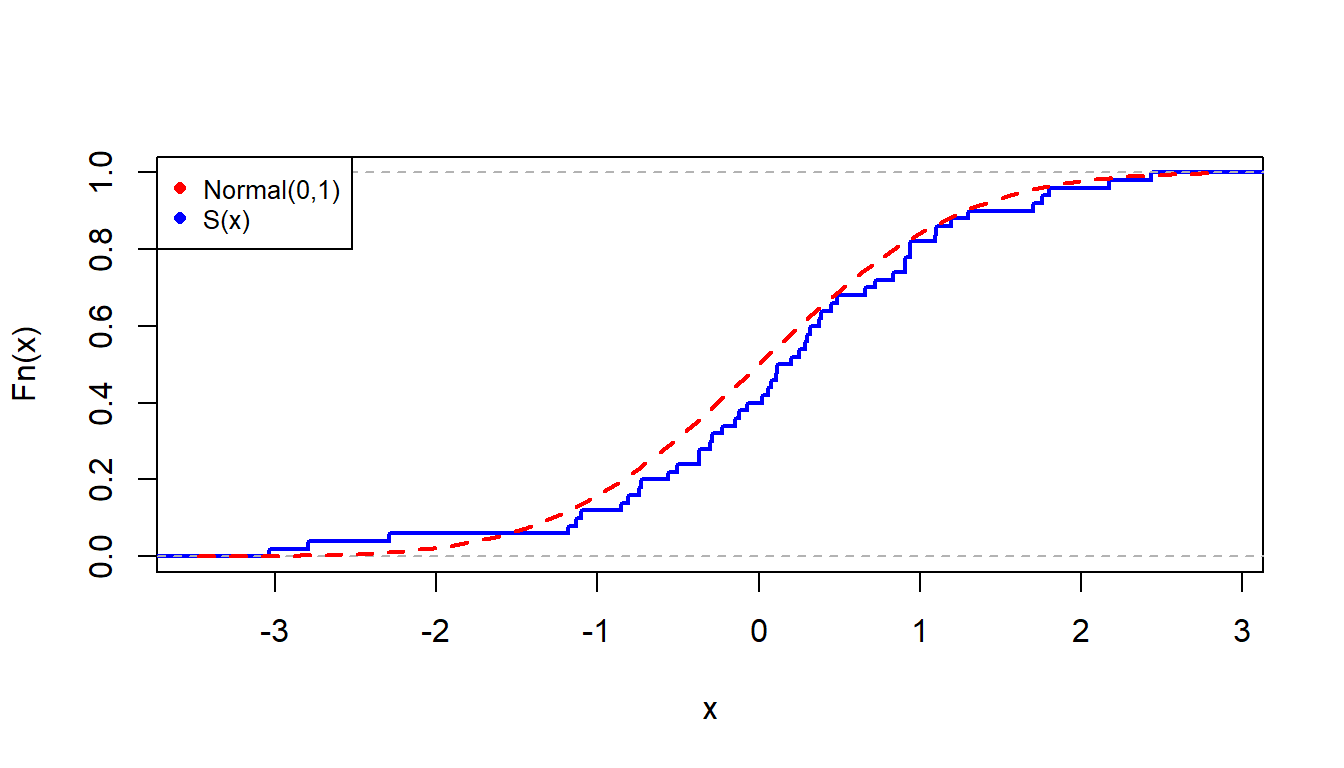
\includegraphics{_main_files/figure-latex/unnamed-chunk-64-1} \end{center}

\begin{Shaded}
\begin{Highlighting}[]
\CommentTok{\#Prueba}
\FunctionTok{library}\NormalTok{(nortest) }
\NormalTok{T1}\OtherTok{\textless{}{-}}\FunctionTok{lillie.test}\NormalTok{(x)}
\NormalTok{T1}
\end{Highlighting}
\end{Shaded}

\begin{verbatim}
    Lilliefors (Kolmogorov-Smirnov) normality test

data:  x
D = 0.08739, p-value = 0.4436
\end{verbatim}

Observamos que la estadística de prueba tiene un valor de 0.08739 y su correspondiente p-value es \(44.36\%\), por lo tanto no rechazaremos \(H_0\) y concluimos no existe evidencia suficiente para suponer que la distribución de la muestra no es \(N(0,1)\). Esperabamos que la prueba diera ese resultado ya que por construcción la muestra proviene de una distribucion \(N(0,1)\).

\hypertarget{pueba-de-lilliefors-exponencial}{%
\chapter{Pueba de Lilliefors Exponencial}\label{pueba-de-lilliefors-exponencial}}

Otro problema importante de bondad de ajuste es la prueba para la distribución exponencial con media no especificada. Este problema es importante porque el supuesto de una distribución exponencial con media desconocida tiene muchas aplicaciones, particularmente donde las variables aleatorias bajo estudio representan el tiempo de espera o el tiempo en que ocurre cierto evento.
Lilliefors en 1969 desarrolló una prueba análoga a la prueba de Kolmogorov-Smirnov y dió una tabla de valores críticos basados en simulaciones Monte Carlo.

\hypertarget{datos-17}{%
\section{Datos}\label{datos-17}}

Los datos consisten en una muestra aleatoria \(X_{1},X_{2},\ldots,X_{n}\) de tamaño \(n\) que sigue una distribución exponencial con media \(\hat{\lambda} = \frac{1}{\overline{X}}\),el cual corresponde al estimador puntual de la media.

Después calcularemos los valores de muestra \(Z_{i}\) definidos por:

\[Z_{i}=\frac{X_{i}}{\overline{X}} \ \ \ \ i=1,2,\ldots,n\]

El estadístico de prueba se calcula a partir de \(Z_{i}s\) en lugar de a partir de la muestra aleatoria. original.

\hypertarget{supuestos-15}{%
\section{Supuestos}\label{supuestos-15}}

\begin{enumerate}
\def\labelenumi{\arabic{enumi})}
\tightlist
\item
  La muestra es una muestra aleatoria.
\end{enumerate}

\hypertarget{hipuxf3tesis-17}{%
\section{Hipótesis}\label{hipuxf3tesis-17}}

\[\textbf{H}_0: \ \mbox{La muestra aleatoria proviene de una población con distribución exponencial:}\]

\[
\textbf{F(x)=} \left\{
\begin{array}{lcc}
1-e^{-\frac{x}{\lambda}} & si & x > 0 \\
x & si &  x < 0 \\
\end{array}
\right.
\]

Donde \(\lambda\) es un parámetro desconocido.

\[vs\]

\[\textbf{H}_a: \ \mbox{La función de distribución de las} \ \  X_{i}s \ \  \mbox{no es exponencial.}\]

\hypertarget{estadistico-de-prueba}{%
\section{Estadistico de Prueba}\label{estadistico-de-prueba}}

El estadístico de prueba está dada por la máxima distancia vertical:

\[T_{2}=\underset{x}{sup} \ | \ F^*(x)-S(x) \ |\]

\hypertarget{regla-de-decisiuxf3n-33}{%
\subsubsection*{Regla de Decisión}\label{regla-de-decisiuxf3n-33}}


Rechazo \(H_0\) a un nivel de significancia \(\alpha\) si \(T_{2}> W_{1-\alpha}\) donde \(W_{1-\alpha}\) es el cuantil obtenido en las tablas correspondientes a nuestra prueba.

\hypertarget{ejemplo-16}{%
\section{Ejemplo}\label{ejemplo-16}}

Dada la siguiente muestra

\[0.4976,\ 1.2514,\ 0.6619,\ 0.561,\ 1.0026,\ 0.3529,\ 0.8595,\ 1.6254,\]
\[1.1514,\ 1.5181,\ 0.8642,\ 0.5206,\ 0.4229,\ 0.9825,\ 1.0183.\]

Se desea probar si la muestra sigue una distribución exponencial con parámetro \(\lambda\) desconocido.

Realizar la prueba con un nivel de significancia del \(95\%\).

\textbf{Paso 1} Prueba a utilizar \textbf{Prueba de Bondad de Ajuste Lilliefors Exponencial}

\textbf{Paso 2} Planteamiento de Hipótesis

\[\textbf{H}_0: \ \mbox{La muestra aleatoria proviene de una población con distribución exponencial}\]

\[\mbox{con} \ \  \lambda \ \  \mbox{parámetro desconocido.}\]

\[vs\]

\[\textbf{H}_a: \ \mbox{La función de distribución de las} \ \  X_{i}s \ \  \mbox{no es exponencial.}\]

\textbf{Paso 3} Estadístico de Prueba

\[T_{2}=\underset{z}{sup} \ | \ F^*(z)-S(z) \ |\]

\textbf{Paso 4} Procedimiento completo para el cálculo del Estadístico de Prueba:

\begin{enumerate}
\def\labelenumi{\arabic{enumi})}
\item
  Se procede a ordenar nuestras observaciones de menor a mayor.
\item
  Se obtiene el estimador puntual de la distribución exponencial con los datos de la muestra, por lo que el parámetro \(\lambda\) es calculado como:
\end{enumerate}

\[\hat{\lambda}=\frac{1}{\overline{X}}=\frac{1}{0.88602}; \ \ \ \ \ \  \overline{X}=\frac{1}{n}\sum_{i=1}^{n}X_{i}=\frac{1}{15}\sum_{i=1}^{15}X_{i}=0.88602\]
3) Después calcularemos los valores de muestra \(Z_{i}\) definidos por:

\[Z_{i}=\frac{X_{i}}{\overline{X}} \ \ \ \ i=1,2,\ldots,15\]

\begin{enumerate}
\def\labelenumi{\arabic{enumi})}
\setcounter{enumi}{3}
\tightlist
\item
  Se calcula la función empírica, como no tenemos ningún valor repetido:
\end{enumerate}

\[S_{n}= \frac{i}{n}=\frac{1}{15},\frac{2}{15}, \ldots, 1. \]

\begin{enumerate}
\def\labelenumi{\arabic{enumi})}
\setcounter{enumi}{4}
\tightlist
\item
  Se calcula la función empírica menos un valor, es decir,
\end{enumerate}

\[S_{n}= \frac{i-1}{n}=\frac{0}{15},\frac{1}{15}, \ldots, \frac{14}{15}.\]

\begin{enumerate}
\def\labelenumi{\arabic{enumi})}
\setcounter{enumi}{5}
\tightlist
\item
  Se calcula \(D^+\) que es el resultado de la resta de la distribución conocida menos la distribución empírica, es decir:
\end{enumerate}

\[D^+= max \ \{ \ S_{n}(Z_{i})-F^*(Z_{i}) \ \}\]

\begin{enumerate}
\def\labelenumi{\arabic{enumi})}
\setcounter{enumi}{6}
\tightlist
\item
  Se calcula \(D^-\) que es el resultado de la resta de la distribución empírica menos uno menos la distribución conocida, es decir:
\end{enumerate}

\[D^-= max \  \{\ S_{n}(Z_{i-1})-F^*(Z_{i}) \ \}\]

\begin{enumerate}
\def\labelenumi{\arabic{enumi})}
\setcounter{enumi}{7}
\tightlist
\item
  Finalmente realizada la tabla, se calcula el máximo de las columnas \(D^+\) y \(D^-\) de ésta manera, se tiene la siguiente tabla:
\end{enumerate}

\(i\)

\(X\)

\(X_i\)

\(Z_i=\frac{X_i}{\bar{x}}\)

\(S_n(Z_i)\)

\(S_n(Z_{i-1})\)

\(F^*(Z_i)\)

\(D^+=S_n(Z_i)-F^*(Z_i)\)

\(D^-=S_n(Z_{i-1})-F^*(Z_i)\)

1

0.4976

0.3529

0.3982

0.0666667

0.0000000

0.3285

-0.2618

-0.3285

2

1.2514

0.4229

0.4773

0.1333333

0.0666667

0.3795

-0.2462

-0.3128

3

0.6619

0.4976

0.5616

0.2000000

0.1333333

0.4297

-0.2297

-0.2963

4

0.5610

0.5206

0.5875

0.2666667

0.2000000

0.4443

-0.1776

-0.2443

5

1.0026

0.5610

0.6331

0.3333333

0.2666667

0.4690

-0.1357

-0.2024

6

0.3529

0.6619

0.7470

0.4000000

0.3333333

0.5262

-0.1262

-0.1929

7

0.8595

0.8595

0.9700

0.4666667

0.4000000

0.6209

-0.1542

-0.2209

8

1.6254

0.8642

0.9753

0.5333333

0.4666667

0.6229

-0.0896

-0.1562

9

1.1514

0.9825

1.1088

0.6000000

0.5333333

0.6700

-0.0700

-0.1367

10

1.5181

1.0026

1.1315

0.6666667

0.6000000

0.6774

-0.0108

-0.0774

11

0.8642

1.0183

1.1492

0.7333333

0.6666667

0.6831

0.0501

-0.0164

12

0.5206

1.1514

1.2995

0.8000000

0.7333333

0.7273

0.0726

0.0059

13

0.4229

1.2514

1.4123

0.8666667

0.8000000

0.7564

0.1102

0.0435

14

0.9825

1.5181

1.7133

0.9333333

0.8666667

0.8197

0.1135

0.0469

15

1.0183

1.6254

1.8344

1.0000000

0.9333333

0.8403

0.1596

0.0930

\begin{enumerate}
\def\labelenumi{\arabic{enumi})}
\setcounter{enumi}{8}
\tightlist
\item
  Entonces
\end{enumerate}

\[ D^+= max \ \  \{\ S_{n}(Z_{i})-F^*(Z_{i}) \ \}= 0.1596 \ \ \ \ y\ \ \ \ D^-= max\  \{ \ S_{n}(Z_{i-1})-F^*(Z_{i}) \ \}=0.0930 \]
Por lo tanto:

\[T_{2}=\underset{z}{sup}\ | \ S_{n}(z)-F^*(z) \ |=max \ \{\ D^+,D^- \ \}=max \ \{ \ 0.1596,0.0930 \ \}=0.1596 \]

\textbf{Paso 5} Regla de Decisión

Este último resultado se compara con la tabla de valores críticos de la Tabla Lilliefors Exponencial, para un nivel de significancia \(\alpha\) = 0.05 \(W_{0.05}\)=0.2776, de esta manera se tiene que \(0.2776 = W_{0.05} > T_{2} = 0.1596\), como el cuantil \(W_{0.05}\)=0.2776 es mayor a comparación de \(T_{2}\)=0.2776.

No Rechazamos \(H_0\).

\textbf{Paso 6} Conclusión

Podemos concluir que a un nivel de significancia \(\alpha\)=0.05, no existe evidencia estadística suficiente para decir que la muestra no tiene distribución exponencial.

\hypertarget{ejemplo-en-r-studio-16}{%
\section{Ejemplo en R-Studio}\label{ejemplo-en-r-studio-16}}

Ahora haremos la réplica en R.

\begin{Shaded}
\begin{Highlighting}[]
\CommentTok{\#Datos}
\NormalTok{i}\OtherTok{=}\DecValTok{1}\SpecialCharTok{:}\DecValTok{15}
\NormalTok{X}\OtherTok{=}\FunctionTok{c}\NormalTok{(}\FloatTok{0.4976}\NormalTok{, }\FloatTok{1.2514}\NormalTok{, }\FloatTok{0.6619}\NormalTok{, }\FloatTok{0.561}\NormalTok{, }\FloatTok{1.0026}\NormalTok{, }\FloatTok{0.3529}\NormalTok{, }\FloatTok{0.8595}\NormalTok{, }\FloatTok{1.6254}\NormalTok{,}
                             \FloatTok{1.1514}\NormalTok{, }\FloatTok{1.5181}\NormalTok{, }\FloatTok{0.8642}\NormalTok{, }\FloatTok{0.5206}\NormalTok{, }\FloatTok{0.4229}\NormalTok{, }\FloatTok{0.9825}\NormalTok{, }\FloatTok{1.0183}\NormalTok{)}
\NormalTok{X\_i}\OtherTok{=}\FunctionTok{c}\NormalTok{(}\FloatTok{0.3529}\NormalTok{,}\FloatTok{0.4229}\NormalTok{,}\FloatTok{0.4976}\NormalTok{,}\FloatTok{0.5206}\NormalTok{,}\FloatTok{0.5610}\NormalTok{, }\FloatTok{0.6619}\NormalTok{,}\FloatTok{0.8595}\NormalTok{,}\FloatTok{0.8642}\NormalTok{,}\FloatTok{0.9825}\NormalTok{,}\FloatTok{1.0026}\NormalTok{,}\FloatTok{1.0183}\NormalTok{,}
      \FloatTok{1.1514}\NormalTok{,}\FloatTok{1.2514}\NormalTok{,}\FloatTok{1.5181}\NormalTok{,}\FloatTok{1.6254}\NormalTok{)}
\NormalTok{Z\_i}\OtherTok{=}\FunctionTok{c}\NormalTok{(}\FloatTok{0.3982}\NormalTok{, }\FloatTok{0.4773}\NormalTok{, }\FloatTok{0.5616}\NormalTok{,}\FloatTok{0.5875}\NormalTok{,}\FloatTok{0.6331}\NormalTok{,}\FloatTok{0.7470}\NormalTok{,}\FloatTok{0.9700}\NormalTok{,}\FloatTok{0.9753}\NormalTok{,}\FloatTok{1.1088}\NormalTok{,}\FloatTok{1.1315}\NormalTok{,}\FloatTok{1.1492}\NormalTok{,}
      \FloatTok{1.2995}\NormalTok{,}\FloatTok{1.4123}\NormalTok{,}\FloatTok{1.7133}\NormalTok{,}\FloatTok{1.8344}\NormalTok{) }
\NormalTok{Sn\_Zi}\OtherTok{=}\FunctionTok{c}\NormalTok{(}\DecValTok{1}\SpecialCharTok{/}\DecValTok{15}\NormalTok{,}\DecValTok{2}\SpecialCharTok{/}\DecValTok{15}\NormalTok{,}\DecValTok{3}\SpecialCharTok{/}\DecValTok{15}\NormalTok{,}\DecValTok{4}\SpecialCharTok{/}\DecValTok{15}\NormalTok{,}\DecValTok{5}\SpecialCharTok{/}\DecValTok{15}\NormalTok{,}\DecValTok{6}\SpecialCharTok{/}\DecValTok{15}\NormalTok{,}\DecValTok{7}\SpecialCharTok{/}\DecValTok{15}\NormalTok{,}\DecValTok{8}\SpecialCharTok{/}\DecValTok{15}\NormalTok{,}\DecValTok{9}\SpecialCharTok{/}\DecValTok{15}\NormalTok{,}\DecValTok{10}\SpecialCharTok{/}\DecValTok{15}\NormalTok{,}\DecValTok{11}\SpecialCharTok{/}\DecValTok{15}\NormalTok{,}\DecValTok{12}\SpecialCharTok{/}\DecValTok{15}\NormalTok{,}\DecValTok{13}\SpecialCharTok{/}\DecValTok{15}\NormalTok{,}\DecValTok{14}\SpecialCharTok{/}\DecValTok{15}\NormalTok{,}\DecValTok{1}\NormalTok{)}
\NormalTok{Sn\_Zi\_1}\OtherTok{=}\FunctionTok{c}\NormalTok{(}\DecValTok{0}\SpecialCharTok{/}\DecValTok{15}\NormalTok{,}\DecValTok{1}\SpecialCharTok{/}\DecValTok{15}\NormalTok{,}\DecValTok{2}\SpecialCharTok{/}\DecValTok{15}\NormalTok{,}\DecValTok{3}\SpecialCharTok{/}\DecValTok{15}\NormalTok{,}\DecValTok{4}\SpecialCharTok{/}\DecValTok{15}\NormalTok{,}\DecValTok{5}\SpecialCharTok{/}\DecValTok{15}\NormalTok{,}\DecValTok{6}\SpecialCharTok{/}\DecValTok{15}\NormalTok{,}\DecValTok{7}\SpecialCharTok{/}\DecValTok{15}\NormalTok{,}\DecValTok{8}\SpecialCharTok{/}\DecValTok{15}\NormalTok{,}\DecValTok{9}\SpecialCharTok{/}\DecValTok{15}\NormalTok{,}\DecValTok{10}\SpecialCharTok{/}\DecValTok{15}\NormalTok{,}\DecValTok{11}\SpecialCharTok{/}\DecValTok{15}\NormalTok{,}\DecValTok{12}\SpecialCharTok{/}\DecValTok{15}\NormalTok{,}\DecValTok{13}\SpecialCharTok{/}\DecValTok{15}\NormalTok{,}\DecValTok{14}\SpecialCharTok{/}\DecValTok{15}\NormalTok{)}
\NormalTok{F\_Zi}\OtherTok{=}\FunctionTok{c}\NormalTok{(}\FloatTok{0.3285}\NormalTok{,}\FloatTok{0.3795}\NormalTok{,}\FloatTok{0.4297}\NormalTok{,}\FloatTok{0.4443}\NormalTok{,}\FloatTok{0.4690}\NormalTok{,}\FloatTok{0.5262}\NormalTok{,}\FloatTok{0.6209}\NormalTok{,}\FloatTok{0.6229}\NormalTok{,}\FloatTok{0.6700}\NormalTok{,}\FloatTok{0.6774}\NormalTok{,}\FloatTok{0.6831}\NormalTok{,}
       \FloatTok{0.7273}\NormalTok{,}\FloatTok{0.7564}\NormalTok{,}\FloatTok{0.8197}\NormalTok{, }\FloatTok{0.8403}\NormalTok{)}
\NormalTok{D\_mas}\OtherTok{=}\FunctionTok{c}\NormalTok{(}\SpecialCharTok{{-}}\FloatTok{0.2618}\NormalTok{,}\SpecialCharTok{{-}}\FloatTok{0.2462}\NormalTok{,}\SpecialCharTok{{-}}\FloatTok{0.2297}\NormalTok{,}\SpecialCharTok{{-}}\FloatTok{0.1776}\NormalTok{,}\SpecialCharTok{{-}}\FloatTok{0.1357}\NormalTok{,}\SpecialCharTok{{-}}\FloatTok{0.1262}\NormalTok{,}\SpecialCharTok{{-}}\FloatTok{0.1542}\NormalTok{,}\SpecialCharTok{{-}}\FloatTok{0.0896}\NormalTok{,}\SpecialCharTok{{-}}\FloatTok{0.0700}\NormalTok{,}
        \SpecialCharTok{{-}}\FloatTok{0.0108}\NormalTok{,}\FloatTok{0.0501}\NormalTok{,}\FloatTok{0.0726}\NormalTok{,}\FloatTok{0.1102}\NormalTok{,}\FloatTok{0.1135}\NormalTok{,}\FloatTok{0.1596}\NormalTok{)}
\NormalTok{D\_menos}\OtherTok{=}\FunctionTok{c}\NormalTok{(}\SpecialCharTok{{-}}\FloatTok{0.3285}\NormalTok{,}\SpecialCharTok{{-}}\FloatTok{0.3128}\NormalTok{,}\SpecialCharTok{{-}}\FloatTok{0.2963}\NormalTok{,}\SpecialCharTok{{-}}\FloatTok{0.2443}\NormalTok{, }\SpecialCharTok{{-}}\FloatTok{0.2024}\NormalTok{,}\SpecialCharTok{{-}}\FloatTok{0.1929}\NormalTok{,}\SpecialCharTok{{-}}\FloatTok{0.2209}\NormalTok{,}\SpecialCharTok{{-}}\FloatTok{0.1562}\NormalTok{,}
           \SpecialCharTok{{-}}\FloatTok{0.1367}\NormalTok{,}\SpecialCharTok{{-}}\FloatTok{0.0774}\NormalTok{,}\SpecialCharTok{{-}}\FloatTok{0.0164}\NormalTok{,}\FloatTok{0.0059}\NormalTok{,}\FloatTok{0.0435}\NormalTok{,}\FloatTok{0.0469}\NormalTok{,}\FloatTok{0.0930}\NormalTok{)  }

\NormalTok{Tabla}\OtherTok{=}\FunctionTok{cbind}\NormalTok{(i,X\_i,Z\_i,Sn\_Zi,Sn\_Zi\_1,F\_Zi,D\_mas,D\_menos)                                                                                                                                                      }
\NormalTok{Tabla}
\end{Highlighting}
\end{Shaded}

\begin{verbatim}
       i    X_i    Z_i      Sn_Zi    Sn_Zi_1   F_Zi   D_mas D_menos
 [1,]  1 0.3529 0.3982 0.06666667 0.00000000 0.3285 -0.2618 -0.3285
 [2,]  2 0.4229 0.4773 0.13333333 0.06666667 0.3795 -0.2462 -0.3128
 [3,]  3 0.4976 0.5616 0.20000000 0.13333333 0.4297 -0.2297 -0.2963
 [4,]  4 0.5206 0.5875 0.26666667 0.20000000 0.4443 -0.1776 -0.2443
 [5,]  5 0.5610 0.6331 0.33333333 0.26666667 0.4690 -0.1357 -0.2024
 [6,]  6 0.6619 0.7470 0.40000000 0.33333333 0.5262 -0.1262 -0.1929
 [7,]  7 0.8595 0.9700 0.46666667 0.40000000 0.6209 -0.1542 -0.2209
 [8,]  8 0.8642 0.9753 0.53333333 0.46666667 0.6229 -0.0896 -0.1562
 [9,]  9 0.9825 1.1088 0.60000000 0.53333333 0.6700 -0.0700 -0.1367
[10,] 10 1.0026 1.1315 0.66666667 0.60000000 0.6774 -0.0108 -0.0774
[11,] 11 1.0183 1.1492 0.73333333 0.66666667 0.6831  0.0501 -0.0164
[12,] 12 1.1514 1.2995 0.80000000 0.73333333 0.7273  0.0726  0.0059
[13,] 13 1.2514 1.4123 0.86666667 0.80000000 0.7564  0.1102  0.0435
[14,] 14 1.5181 1.7133 0.93333333 0.86666667 0.8197  0.1135  0.0469
[15,] 15 1.6254 1.8344 1.00000000 0.93333333 0.8403  0.1596  0.0930
\end{verbatim}

\begin{Shaded}
\begin{Highlighting}[]
\NormalTok{EstPrueba}\OtherTok{=}\FunctionTok{max}\NormalTok{(D\_mas,D\_menos)}
\NormalTok{EstPrueba}
\end{Highlighting}
\end{Shaded}

\begin{verbatim}
[1] 0.1596
\end{verbatim}

\begin{Shaded}
\begin{Highlighting}[]
\NormalTok{EstdPrueba}
\end{Highlighting}
\end{Shaded}

\begin{verbatim}
[1] 0.2179
\end{verbatim}

El cuantil W que acumula \(1-\alpha\) de probabilidad, usando \(\alpha=0.05\) es \(W = 0.2776\), encontrado en las tablas correspondientes. Por lo tanto tenemos que \(T1=0.1596 < W=0.2776\), entonces rechazamos la hipotesis nula. Y concluimos que hay evidencia suficiente para decir que la muestra no proviene de una distribución exponencial.

\begin{Shaded}
\begin{Highlighting}[]
\FunctionTok{library}\NormalTok{(nortest) }\CommentTok{\#prueba lilliefors}
\FunctionTok{lillie.test}\NormalTok{(F\_Zi) }\CommentTok{\#Ocupamos estos datos ya que debemos recordar que }
\end{Highlighting}
\end{Shaded}

\begin{verbatim}
    Lilliefors (Kolmogorov-Smirnov) normality test

data:  F_Zi
D = 0.15238, p-value = 0.458
\end{verbatim}

\begin{Shaded}
\begin{Highlighting}[]
                   \CommentTok{\#es una distribución exponencial y F\_Zi son datos estandarizados }
\end{Highlighting}
\end{Shaded}

\hypertarget{prueba-anderson-darling}{%
\chapter{Prueba Anderson-Darling}\label{prueba-anderson-darling}}

La prueba de Anderson Darling, al igual que la prueba de Lilliefors sirve para probar la
hipótesis de que una muestra aleatoria sigue una cierta distribución especificada.

\hypertarget{datos-18}{%
\section{Datos}\label{datos-18}}

Los datos consisten en una muestra aleatoria \(X_{1},X_{2},\ldots,X_{n}\) de tamaño \(n\) asociada con alguna función de distribución desconocida, denotada por \(F(x)\).

\hypertarget{supuestos-16}{%
\section{Supuestos}\label{supuestos-16}}

\begin{itemize}
\tightlist
\item
  La muestra es una muestra aleatoria.
\end{itemize}

\hypertarget{hipuxf3tesis-18}{%
\section{Hipótesis}\label{hipuxf3tesis-18}}

\hypertarget{caso-a-prueba-de-2-colas-solo-seruxe1-este-caso}{%
\subsection*{Caso A (Prueba de 2 colas) Solo será este caso}\label{caso-a-prueba-de-2-colas-solo-seruxe1-este-caso}}


\[\textbf{H}_0: \ F(x)=F^*(x) \ \ \ \ \forall\ \ x\  \mbox{de} \ \ -\infty \ \ \mbox{a} \ \  +\infty\]

\[vs\]

\[\textbf{H}_a: \ F(x) \neq F^*(x) \ \ \ \ \mbox{para al menos un  valor de} \  x.\]

Donde \(F^*(x)\) es la distribución teórica que se quiere probar con un nivel de significancia \(\alpha\).

Para probar dicha hipótesis Anderson propone examinar las diferencias al cuadrados entre la distribución empírica de los datos \(S_{n}(X)\) y la distribución teórica propuesta y completamente
especificada \(F^*(X)\) y luego integrar respecto a la distribución propuesta.
A este tipo de pruebas se les conoce como funciones de distribución empíricas cuadráticas \textbf{(QEDF)} por
sus siglas en inglés.
De esta manera la estadística de la prueba \textbf{Anderson-Darling} se obtiene de integrar la
siguiente función \textbf{QEDF}:

\[A_n^2=n \int_{-\infty}^{\infty} (Sn(X)-F^*(X))^2 \frac{1}{F^*(X)(1-F^*(X))}\]

Una característica importante es que se usa la expresión \(\frac{1}{F^*(X)(1-F^*(X))}\)
debido a que se busca que las colas de distribución tengan un peso cuantificablemente mayor, con la finalidad de detectar diferencias en las colas de la distribución.

\hypertarget{estaduxedstico-de-prueba-16}{%
\section{Estadístico de Prueba}\label{estaduxedstico-de-prueba-16}}

Resolviendo la integral se obtiene la estadístico de la forma:

\[A_n^2=-n-\frac{1}{n}\sum_{i=1}^{n}\left(2i-1\right) \ [ \ ln(F^*(X_{(i)})) +ln(1-F^*(X_{(n-i+1)})) \ ]\]

Dado que el estadístico no depende de \(F(X)\) y sólo depende de \(n\) entonces la distribución
asintótica de \textbf{Anderson-Darling} es la que se muestra a continuación, asimismo se mostrarán algunos
ajustes a la estadística con la finalidad de que la prueba sea más potente para determinados
casos:

\[
\begin{array}{|c c| c c c c|}
\hline
\textbf{Caso} & \textbf{Ajuste en el estadístico} &\textbf{0.90} &\textbf{0.95} & \textbf{0.975} & \textbf{0.99} \\
\hline
\mbox{Todos los parámetros conocidos} & A_{n}^{2} \ \ para\ n\ \geq 5 & 1.933 & 2.492 & 3.070 & 3.857 \\
Normal\ con\ N(\overline{X},S^2) & (1+\frac{4}{n}+\frac{25}{n^2})A_{n}^{2} & 0.632 & 0.751 & 0.870 & 1.029 \\
\mbox{Exponencial con} \ \ exp(\overline{X}) & (1+\frac{0.6}{n})A_{n}^{2} & 1.070 & 1.326 & 1.587 & 1.943 \\
\mbox{Weibull con} \ \ Weibull(\hat{\alpha},\hat{\beta}) & (1+\frac{0.2}{\sqrt{n}})A_{n}^{2} & 0.637 & 0.757 & 0.877 & 1.038 \\
\mbox{Log-logística con} \ \ Log-log(\hat{\alpha},\hat{\beta}) & (1+\frac{0.25}{\sqrt{n}})A_{n}^{2} & 0.563 & 0.660 & 0.769 & 0.906 \\
\hline
\end{array}
\]

\hypertarget{regla-de-decisiuxf3n-34}{%
\section{Regla de Decisión}\label{regla-de-decisiuxf3n-34}}

Rechazo \(H_0\) a un nivel de significancia \(\alpha\) si \(A_{n}^2> A_{1-\alpha}\) donde \(A_{n}^{2}\) ya tiene el ajuste para cada caso mencionado anteriormente y \(A_{1-\alpha}\) es el cuantil obtenido en las tablas correspondientes a nuestra prueba.

Para ejemplificar la prueba de \(Anderson-Darling\) veamos el siguiente ejemplo:

\hypertarget{ejemplo-17}{%
\subsection{Ejemplo}\label{ejemplo-17}}

Se desea probar si la siguiente muestra:

\[-4.1302,\ \ 9.315,\ \ 3.9757,\ \ 8.49,\ \ 5.6204,\ \ -6.9098,\ \ -0.1426,\ \ -2.3838,\]
\[-2.0039,\ \ 1.7349,\ \ 5.7442,\ \ 2.7931,\ \ 6.2938,\ \ 11.7337,\ \ -0.1318.\]

Sigue una distribución Normal, para ello se realizará la prueba de Anderson Darling con un nivel de significancia del \(5\%\).

\textbf{Paso 1} Prueba a utilizar \textbf{Prueba de Bondad de Ajuste Anderson-Darling}

\textbf{Paso 2} Planteamiento de Hipótesis

\[\textbf{H}_0: \ \mbox{La muestra} \ \sim \  N(\mu,\sigma^2).\]

\[vs\]

\[\textbf{H}_a: \ \mbox{La muestra} \ \ \nsim \ \  N(\mu,\sigma^2).\]

\textbf{Paso 3} Estadístico de Prueba

\[A_n^2=-n-\frac{1}{n}\sum_{i=1}^{n}\left(2i-1\right)[ \ ln(F^*(X_{(i)})) +ln(1-F^*(X_{(n-i+1)})) \ ]\]

\textbf{Paso 4} Procedimiento completo para el cálculo del Estadístico de Prueba:

\begin{enumerate}
\def\labelenumi{\arabic{enumi})}
\item
  Se procede a ordenar nuestras observaciones de menor a mayor.
\item
  Se obtienen los estimadores puntuales de distribución normal con los datos de la muestra,
  \(\overline{X}=\frac{1}{n}\sum_{i=1}^{n}X_{i}= 2.66658\) y \(s=\sqrt{\frac{1}{n-1}\sum_{i=1}^{n}(X_{i}-\overline{X})^2}=5.313212\)
\item
  Se calcula la distribución propuesta, en este caso una distribución normal con media \(\overline{X}\) y varianza \(s^2\), es decir,\(F^*(X)\), para ello se usa la aproximación a una normal estándar
\item
  Se calcula el primer sumando \(ln(F^*(X_{(i)}))\) el cual se denotará como \(L1\), después se calculará el segundo sumando \(ln(1-F^*(X_{(n-i+1)}))\) el cual se denotará como \(L2\)
\item
  Se realiza el sumando de manera puntal, es decir, calcular:
\end{enumerate}

\[Q_{i}=\left(\frac{2i-1}{n}\right)[ \ ln(F^*(X_{(i)})) +ln(1-F^*(X_{(n-i+1)})) \ ] \ \ \ \mbox{para} \  i=1,\ldots,15.\]

\begin{enumerate}
\def\labelenumi{\arabic{enumi})}
\setcounter{enumi}{5}
\tightlist
\item
  Y se realiza la siguiente tabla:
\end{enumerate}

\(i\)

\(X\)

\(X_i\)

\(F*(X_i)\)

\(L_1=ln(F*(X_i))\)

\(L_2=ln(1-F*(X_n-i+1))\)

Qi

1

-4.1302

-6.9098

0.0357

-3.3313

-3.1245

-0.4303

2

9.3150

-4.1302

0.1004

-2.2984

-2.2498

-0.9096

3

3.9757

-2.3838

0.1709

-1.7665

-1.9911

-1.2525

4

8.4900

-2.0039

0.1896

-1.6623

-1.3967

-1.4275

5

5.6204

-0.1426

0.2985

-1.2089

-1.2686

-1.4865

6

-6.9098

-0.1318

0.2992

-1.2066

-1.2408

-1.7948

7

-0.1426

1.7349

0.4304

-0.8430

-0.9095

-1.5189

8

-2.3838

2.7931

0.5094

-0.6743

-0.7123

-1.3866

9

-2.0039

3.9757

0.5973

-0.5153

-0.5628

-1.2218

10

1.7349

5.6204

0.7108

-0.3412

-0.3555

-0.8826

11

5.7442

5.7442

0.7187

-0.3301

-0.3545

-0.9586

12

2.7931

6.2938

0.7525

-0.2842

-0.2103

-0.7583

13

6.2938

8.4900

0.8634

-0.1468

-0.1874

-0.5570

14

11.7337

9.3150

0.8945

-0.1113

-0.1058

-0.3909

15

-0.1318

11.7337

0.9560

-0.0449

-0.0363

-0.1572

\begin{enumerate}
\def\labelenumi{\arabic{enumi})}
\setcounter{enumi}{6}
\tightlist
\item
  Finalmente se suma todos los \(Q_{i}s\) y se construye el estadístico:
\end{enumerate}

\[A_n^2=-n-\sum_{i=1}^{n}Qi=-n-\frac{1}{n}\sum_{i=1}^{n}\left(2i-1\right)[ \ ln(F^*(X_{(i)})) +ln(1-F^*(X_{(n-i+1)})) \ ]\]
\[A_n^2=-n-\sum_{i=1}^{n}Qi=-15-(-15.1340)=15.1340-15=0.1340\]

\[A_n^2=0.1340\]

\begin{enumerate}
\def\labelenumi{\arabic{enumi})}
\setcounter{enumi}{7}
\tightlist
\item
  Aplicando el ajuste de la tabla anterior:
  \[
  \begin{array}{|c c| c c c c|}
  \hline
  \textbf{Caso} & \textbf{Ajuste en el estadístico} &\textbf{0.90} &\textbf{0.95} & \textbf{0.975} & \textbf{0.99} \\
  \hline
  \hline
  Normal\ con\ N(\overline{X},S^2) & (1+\frac{4}{n}+\frac{25}{n^2})A_{n}^{2} & 0.632 & 0.751 & 0.870 & 1.029 \\
  \hline
  \end{array}
  \]
\end{enumerate}

\[ (1+\frac{4}{n}+\frac{25}{n^2})A_{n}^{2}=(1+\frac{4}{15}+\frac{25}{15^2})A_{n}^{2}=0.1846\]

\textbf{Paso 5} Regla de Decisión

Este último resultado se compara con la tabla de valores críticos de la Tabla Anderson-Darling para el caso de Normalidad, para un nivel de significancia \(\alpha\) = 0.05.

Por lo anterior \(A_{0.95}\)=0.751, de esta manera se tiene que 0.751 = \(A_{0.95} > A_{n}^2=0.1846\), como el valor crítico \(A_{0.95}\) es mayor a comparación de \(A_{n}^2\)=0.1846.

\(\therefore\) No Rechazamos \(H_0\).

\textbf{Paso 6} Conclusión

Podemos concluir que a un nivel de significancia \(\alpha=0.05\), no existe evidencia estadística suficiente para decir que la muestra no tiene distribución normal.

\hypertarget{ejemplo-en-r-studio-17}{%
\section{Ejemplo en R-Studio}\label{ejemplo-en-r-studio-17}}

Ahora haremos la réplica en R.

\begin{Shaded}
\begin{Highlighting}[]
\CommentTok{\#Datos}
\NormalTok{i}\OtherTok{=}\DecValTok{1}\SpecialCharTok{:}\DecValTok{15}
\NormalTok{n}\OtherTok{=}\DecValTok{15}
\NormalTok{X}\OtherTok{=}\FunctionTok{c}\NormalTok{(}\SpecialCharTok{{-}}\FloatTok{4.1302}\NormalTok{, }\FloatTok{9.315}\NormalTok{, }\FloatTok{3.9757}\NormalTok{, }\FloatTok{8.49}\NormalTok{, }\FloatTok{5.6204}\NormalTok{, }\SpecialCharTok{{-}}\FloatTok{6.9098}\NormalTok{, }\SpecialCharTok{{-}}\FloatTok{0.1426}\NormalTok{, }\SpecialCharTok{{-}}\FloatTok{2.3838}\NormalTok{,}
                            \SpecialCharTok{{-}}\FloatTok{2.0039}\NormalTok{, }\FloatTok{1.7349}\NormalTok{, }\FloatTok{5.7442}\NormalTok{,}\FloatTok{2.7931}\NormalTok{,}\FloatTok{6.2938}\NormalTok{,}\FloatTok{11.7337}\NormalTok{,}\SpecialCharTok{{-}}\FloatTok{0.1318}\NormalTok{)}
\NormalTok{X\_i}\OtherTok{=}\FunctionTok{c}\NormalTok{(}\SpecialCharTok{{-}}\FloatTok{6.9098}\NormalTok{,}\SpecialCharTok{{-}}\FloatTok{4.1302}\NormalTok{,}\SpecialCharTok{{-}}\FloatTok{2.3838}\NormalTok{,}\SpecialCharTok{{-}}\FloatTok{2.0039}\NormalTok{, }\SpecialCharTok{{-}}\FloatTok{0.1426}\NormalTok{,}\SpecialCharTok{{-}}\FloatTok{0.1318}\NormalTok{,}\FloatTok{1.7349}\NormalTok{,}\FloatTok{2.7931}\NormalTok{,}\FloatTok{3.9757}\NormalTok{,}\FloatTok{5.6204}\NormalTok{,}
      \FloatTok{5.7442}\NormalTok{,}\FloatTok{6.2938}\NormalTok{,}\FloatTok{8.4900}\NormalTok{,}\FloatTok{9.3150}\NormalTok{,}\FloatTok{11.7337}\NormalTok{)}
\NormalTok{F\_Xi}\OtherTok{=}\FunctionTok{c}\NormalTok{( }\FloatTok{0.0357}\NormalTok{, }\FloatTok{0.1004}\NormalTok{,}\FloatTok{0.1709}\NormalTok{,}\FloatTok{0.1896}\NormalTok{,}\FloatTok{0.2985}\NormalTok{,}\FloatTok{0.2992}\NormalTok{,}\FloatTok{0.4304}\NormalTok{,}\FloatTok{0.5094}\NormalTok{,}\FloatTok{0.5973}\NormalTok{,}\FloatTok{0.7108}\NormalTok{,}
        \FloatTok{0.7187}\NormalTok{,}\FloatTok{0.7525}\NormalTok{,}\FloatTok{0.8634}\NormalTok{,}\FloatTok{0.8945}\NormalTok{,}\FloatTok{0.9560}\NormalTok{)}
\NormalTok{L1}\OtherTok{=}\FunctionTok{c}\NormalTok{( }\SpecialCharTok{{-}}\FloatTok{3.3313}\NormalTok{,}\SpecialCharTok{{-}}\FloatTok{2.2984}\NormalTok{,}\SpecialCharTok{{-}}\FloatTok{1.7665}\NormalTok{,}\SpecialCharTok{{-}}\FloatTok{1.6623}\NormalTok{,}\SpecialCharTok{{-}}\FloatTok{1.2089}\NormalTok{,}\SpecialCharTok{{-}}\FloatTok{1.2066}\NormalTok{,}\SpecialCharTok{{-}}\FloatTok{0.8430}\NormalTok{,}\SpecialCharTok{{-}}\FloatTok{0.6743}\NormalTok{,}\SpecialCharTok{{-}}\FloatTok{0.5153}\NormalTok{,}\SpecialCharTok{{-}}\FloatTok{0.3412}\NormalTok{,}\SpecialCharTok{{-}}\FloatTok{0.3301}\NormalTok{,}
      \SpecialCharTok{{-}}\FloatTok{0.2842}\NormalTok{,}\SpecialCharTok{{-}}\FloatTok{0.1468}\NormalTok{,}\SpecialCharTok{{-}}\FloatTok{0.1113}\NormalTok{,}\SpecialCharTok{{-}}\FloatTok{0.0449}\NormalTok{)    }\CommentTok{\#ln(F*(Xi))}
\NormalTok{L2}\OtherTok{=}\FunctionTok{c}\NormalTok{(}\SpecialCharTok{{-}}\FloatTok{3.1245}\NormalTok{,}\SpecialCharTok{{-}}\FloatTok{2.2498}\NormalTok{,}\SpecialCharTok{{-}}\FloatTok{1.9911}\NormalTok{,}\SpecialCharTok{{-}}\FloatTok{1.3967}\NormalTok{,}\SpecialCharTok{{-}}\FloatTok{1.2686}\NormalTok{,}\SpecialCharTok{{-}}\FloatTok{1.2408}\NormalTok{,}\SpecialCharTok{{-}}\FloatTok{0.9095}\NormalTok{,}
\SpecialCharTok{{-}}\FloatTok{0.7123}\NormalTok{,}\SpecialCharTok{{-}}\FloatTok{0.5628}\NormalTok{,}\SpecialCharTok{{-}}\FloatTok{0.3555}\NormalTok{,}\SpecialCharTok{{-}}\FloatTok{0.3545}\NormalTok{,}\SpecialCharTok{{-}}\FloatTok{0.2103}\NormalTok{,}\SpecialCharTok{{-}}\FloatTok{0.1874}\NormalTok{,}\SpecialCharTok{{-}}\FloatTok{0.1058}\NormalTok{,}\SpecialCharTok{{-}}\FloatTok{0.0363}\NormalTok{)  }\CommentTok{\#ln(1{-}F*(Xn{-}i+1))}
\NormalTok{Qi}\OtherTok{=}\FunctionTok{c}\NormalTok{(}\SpecialCharTok{{-}}\FloatTok{0.4303}\NormalTok{,}\SpecialCharTok{{-}}\FloatTok{0.9096}\NormalTok{,}\SpecialCharTok{{-}}\FloatTok{1.2525}\NormalTok{,}\SpecialCharTok{{-}}\FloatTok{1.4275}\NormalTok{,}\SpecialCharTok{{-}}\FloatTok{1.4865}\NormalTok{,}\SpecialCharTok{{-}}\FloatTok{1.7948}\NormalTok{,}\SpecialCharTok{{-}}\FloatTok{1.5189}\NormalTok{,}\SpecialCharTok{{-}}\FloatTok{1.3866}\NormalTok{,}\SpecialCharTok{{-}}\FloatTok{1.2218}\NormalTok{,}\SpecialCharTok{{-}}\FloatTok{0.8826}\NormalTok{,}
\SpecialCharTok{{-}}\FloatTok{0.9586}\NormalTok{,}\SpecialCharTok{{-}}\FloatTok{0.7583}\NormalTok{,}\SpecialCharTok{{-}}\FloatTok{0.5570}\NormalTok{,}\SpecialCharTok{{-}}\FloatTok{0.3909}\NormalTok{,}\SpecialCharTok{{-}}\FloatTok{0.1572}\NormalTok{)}

\CommentTok{\#Ahora calcularemos el estadistico de prueba}
\NormalTok{A\_2}\OtherTok{=}\SpecialCharTok{{-}}\NormalTok{n}\SpecialCharTok{{-}}\NormalTok{(}\FunctionTok{sum}\NormalTok{(Qi))}
\NormalTok{A\_2}
\end{Highlighting}
\end{Shaded}

\begin{verbatim}
[1] 0.1331
\end{verbatim}

\begin{Shaded}
\begin{Highlighting}[]
\CommentTok{\#Ahora aplicaremos el ajuste correspondiente}

\NormalTok{A\_2ajust}\OtherTok{=}\NormalTok{(}\DecValTok{1}\SpecialCharTok{+}\DecValTok{4}\SpecialCharTok{/}\NormalTok{n}\SpecialCharTok{+}\DecValTok{25}\SpecialCharTok{/}\NormalTok{n}\SpecialCharTok{\^{}}\DecValTok{2}\NormalTok{)}\SpecialCharTok{*}\NormalTok{A\_2}
\NormalTok{A\_2ajust}
\end{Highlighting}
\end{Shaded}

\begin{verbatim}
[1] 0.1833822
\end{verbatim}

Por la tabla auxiliar tenemos \(A_{0.95}=0.751\), de esta manera se tiene que 0.751 = \(A_{0.95} > A_{n}^2=0.1846\), como el valor crítico \(A_{0.95}\) es mayor a comparación de \(A_{n}^2=0.1846\), entonces no rechazamos \(H_0\). Podemos concluir que a un nivel de significancia \(\alpha\)=0.05, no existe evidencia estadística suficiente para decir que la muestra no tiene distribución normal.

Ahora podemos utilizar la prueba en R

\begin{Shaded}
\begin{Highlighting}[]
\FunctionTok{ad.test}\NormalTok{(X)   }\CommentTok{\#Recordemos que la función no hace el ajuste}
\end{Highlighting}
\end{Shaded}

\begin{verbatim}
    Anderson-Darling test of goodness-of-fit
    Null hypothesis: uniform distribution
    Parameters assumed to be fixed

data:  X
An = Inf, p-value = 4e-05
\end{verbatim}

\hypertarget{otras-estaduxedsticas}{%
\chapter{Otras estadísticas}\label{otras-estaduxedsticas}}

La prueba de Kuiper esta muy relacionada con la prueba Kolmogorov--Smirnov (o prueba K-S). Como la prueba \(K-S\), esta prueba utiliza las estadísticas \(D^+\) y \(D^-\) que representan las diferencias mas positivas y mas negativas entre las distribuciones que se estan comparando. La estadística de prueba de Kuiper es:
\[V=D^+ + D^-\]
Con este pequeño cambio, la prueba de Kuiper es tan sensible en las colas como lo es en la mediana de la distribución.

Las pruebas \textbf{Anderson--Darling} y \textbf{Cramér--von Mises} pertenecen a un grupo llamado \textbf{estadísticas EDF cuadráticas}, en donde el término EDF se refiere a que se basan en la función de distribución empírica.

Este grupo de estadísticas esta definido de la siguiente manera:
\[n\int_{-\infty}^{\infty}(S(x)-F_0(x))^2w(x)dF_0(x)\]
En donde la diferencia entre la distribución empírica y la hipótetica está calculada con el término cuadrático y el término \(w(x)\) es un peso que se da esas diferencias.

Cuando \(w(x)=1\) entonces se tiene la estadística de Cramér--von Mises; cuando \(w(x)=[F_0(x)(1-F_0(x))]^{-1}\) entonces se tiene la estadística de Anderson--Darling, la cual por construcción asigna mayores pesos a observaciones en las colas de la distribución.

En R, la libreria ``goftest'' contiene las pruebas Anderson--Darling y Cramér--von Mises entre otras.

Retomando el ejemplo de las alturas de los pinos, probaremos ahora que las alturas tienen distribución normal y exponencial.

\begin{Shaded}
\begin{Highlighting}[]
\NormalTok{X}\OtherTok{=}\NormalTok{Loblolly}\SpecialCharTok{$}\NormalTok{height}
\NormalTok{meanx}\OtherTok{=}\FunctionTok{mean}\NormalTok{(X)}
\NormalTok{meanx}
\end{Highlighting}
\end{Shaded}

\begin{verbatim}
[1] 32.3644
\end{verbatim}

\begin{Shaded}
\begin{Highlighting}[]
\NormalTok{sdx}\OtherTok{=}\FunctionTok{sd}\NormalTok{(X)}
\NormalTok{sdx}
\end{Highlighting}
\end{Shaded}

\begin{verbatim}
[1] 20.6736
\end{verbatim}

\begin{Shaded}
\begin{Highlighting}[]
\FunctionTok{library}\NormalTok{(goftest)}
\FunctionTok{ad.test}\NormalTok{(X,}\AttributeTok{null =} \StringTok{"pnorm"}\NormalTok{,}\AttributeTok{mean=}\NormalTok{meanx,}\AttributeTok{sd=}\NormalTok{sdx)}
\end{Highlighting}
\end{Shaded}

\begin{verbatim}
    Anderson-Darling test of goodness-of-fit
    Null hypothesis: Normal distribution
    with parameters mean = 32.3644047619048, sd = 20.6736047504145
    Parameters assumed to be fixed

data:  X
An = 2.7319, p-value = 0.03765
\end{verbatim}

\begin{Shaded}
\begin{Highlighting}[]
\FunctionTok{cvm.test}\NormalTok{(X,}\AttributeTok{null =} \StringTok{"pnorm"}\NormalTok{,}\AttributeTok{mean=}\NormalTok{meanx,}\AttributeTok{sd=}\NormalTok{sdx)}
\end{Highlighting}
\end{Shaded}

\begin{verbatim}
    Cramer-von Mises test of goodness-of-fit
    Null hypothesis: Normal distribution
    with parameters mean = 32.3644047619048, sd = 20.6736047504145
    Parameters assumed to be fixed

data:  X
omega2 = 0.38648, p-value = 0.07825
\end{verbatim}

\begin{Shaded}
\begin{Highlighting}[]
\FunctionTok{ad.test}\NormalTok{(X,}\AttributeTok{null =} \StringTok{"pexp"}\NormalTok{,}\AttributeTok{rate=}\DecValTok{1}\SpecialCharTok{/}\NormalTok{meanx)}
\end{Highlighting}
\end{Shaded}

\begin{verbatim}
    Anderson-Darling test of goodness-of-fit
    Null hypothesis: exponential distribution
    with parameter rate = 0.0308981428009166
    Parameters assumed to be fixed

data:  X
An = 4.5223, p-value = 0.004895
\end{verbatim}

\begin{Shaded}
\begin{Highlighting}[]
\FunctionTok{cvm.test}\NormalTok{(X,}\AttributeTok{null =} \StringTok{"pexp"}\NormalTok{,}\AttributeTok{rate=}\DecValTok{1}\SpecialCharTok{/}\NormalTok{meanx)}
\end{Highlighting}
\end{Shaded}

\begin{verbatim}
    Cramer-von Mises test of goodness-of-fit
    Null hypothesis: exponential distribution
    with parameter rate = 0.0308981428009166
    Parameters assumed to be fixed

data:  X
omega2 = 0.79946, p-value = 0.007174
\end{verbatim}

\hypertarget{ejercicios-3}{%
\chapter{Ejercicios}\label{ejercicios-3}}

\textbf{1.} Se lanza un dado 600 veces se obtuvieron los siguientes resultados.

\[
\begin{array}{|c ||c |c |c|c|c|c|}
\hline 
\textbf{Número del dado} & 1& 2& 3&4&5&6 \\
\hline 
\textbf{Observaciones} & 87 &  96 &108&89&122&98 \\
 \hline 
\end{array}
\]

¿El dado está balanceado (es decir, los datos tienen distribución uniforme con proba 1/6)? Use \(\alpha=0.10\)

\textbf{2.} Cierto banco otorga crédito a las personas con una tasa preferencial, de tal manera que los acreditados pueden pagar en cualquier momento desde que piden el préstamo hasta 8 semanas posteriores para que les sea respetada la tasa preferencial. Se seleccionaron aleatoriamente a 1,000 personas y observó su comportamiento de pago, generando de esta manera la siguiente tabla de frecuencia:

\[
\begin{array}{|c|c|  }
\hline
\mbox{Semana}& \mbox{Créditos Pagados}\\
\hline
\mbox{Menos de 1  semana} &64\\
1 \leq x < 2& 191\\
2 \leq  x < 3 &283\\
3 \leq  x < 4 &241\\
4 \leq  x < 5 &140\\
5 \leq  x < 6 &51\\
6 \leq  x < 7 &25\\
7 \leq  x < 8 &4\\
\mbox{8 semanas o más} & 1\\
\hline
\end{array}
\]

Probar que el pago de estos créditos, sigue una distribución binomial con parámetros \(n = 10\) y \(p = 0.25\).

\textbf{3.} Cinco niños de cuarto grado de primaria fueron seleccionados al azar de todos los niños de ese grado en la escuela ``15 de septiembre'', para participar en una carrera. Sus tiempos en segundos fueron: 6.3, 4.2, 4.7, 6.0, y 5.7. Probar con la hipótesis de que los tiempos provienen de una distribución uniforme en el intervalo de 4 a 8 segundos.

\textbf{4.} La siguiente muestra aleatoria hace referencia a los rendimientos positivos de cierta acción a lo largo del tiempo.

0.2513, 0.2566, 0.3459, 0.6379, 2.0505, 1.803, 2.1906,1.5299,
0.35005, 0.3128, 1.2726, 2.3674, 2.3214, 2.4373, 0.6548.

¿Usted piensa que la anterior muestra sigue una distribución normal?

Realizar la prueba correspondiente para verificar que su suposición es cierta con un nivel de confianza del \(90\%\).

\textbf{5.} Se obtuvieron sesenta y dos observaciones de un experimento, y se plantea la pregunta de si dichas observaciones provienen de una distribución normal con media 12 y desviación estándar 3. Ninguna observación se encontró por debajo del cuartil inferior de la distribución, 35 estuvieron por arriba de cuartil superior, 22 tomaron valores menores a la mediana, y 5 estuvieron entre la mediana y el cuartil superior. ¿Es posible concluir que las observaciones provienen de la distribución mencionada?

\textbf{6.} Dada la siguiente muestra

0.6379, 1.5299, 0.35005, 2.0505, 2.1906, 0.3459, 2.3214, 0.3128
0.6548, 2.4373, 1.803, 2.3674, 1.2716, 0.2566, 0.2513.

Se desea hacer el siguiente contraste:

\[\textbf{H}_0: \ \mbox{Los datos} \ \sim LogN(0,1) \ \ vs \ \ \textbf{H}_a: \ mbox{Los datos} \  \nsim \ LogN(0,1)\]

Realice la prueba de Kolmogorov al \(5\%\) de significancia.

\textbf{7.} Se desea probar la hipótesis de que los tiempos entre las llegadas de los pacientes a un hospital con una emergencia se distribuyen exponencial con media \(\bar{x}\). Para ello se registró el tiempo transcurrido entre las llegadas sucesivas de pacientes en una mañana. El tiempo en minutos es el siguiente:

\[
\begin{array}{c c c}
14.3, & 38.0, & 3.8,  \\ 
10.8, & 6.1,& 10.1, \\ 
3.6, & 6.2, & 12.8, \\ 
22.1, & 4.2, & 4.6,  \\ 
1.5, & 3.3, & 1.2,  \\   
20.0, & 7.1,& 8.1.\\
\end{array}
\]

Pruebe la hipótesis con un nivel se significancia del \(5\%\).

\textbf{8.} Se desea probar la hipótesis de que las tasas de interés de un determinado producto financiero tiene el comportamiento de una variable aleatoria como función de distribución normal.

9.1, 5, 7.3, 7.4, 5.5, 8.6, 7, 4.3, 4.7, 8,
4, 8.5, 6.4,6.1, 5.8, 9.5, 5.2, 6.7, 8.3, 9.2.

\textbf{9.} El gerente de una tienda quiere probar la hipótesis de que los clientes llegan aleatoriamente a su tienda, para ello registro el tiempo transcurrido entre las llegadas sucesivas de clientes en una mañana. El tiempo en minutos es el siguiente:

3.6, 6.2, 12.9, 14.2, 38.0, 3.8,\\
10.8, 6.1, 10.1, 22.1, 4.2, 4.6,\\
1.4, 3.3, 8.2.

Pruebe la hipótesis nula de que el tiempo entre las llegadas de los clientes se distribuyen con función de distribución exponencial.

  \bibliography{book.bib,packages.bib}

\end{document}
